\documentclass[MScCS,12pt,oneside,final]{uccthesis}

\addbibresource{mybib.bib} 

\usepackage{listings}
\usepackage{xcolor}
\usepackage{biblatex}
\usepackage{booktabs}
\usepackage{graphicx}
\usepackage{multirow}
\usepackage{tabularx}
\usepackage[hidelinks]{hyperref}


\title{Evaluating the Impact of Buffer Capacity in the onEEGwaveLAD Online Pipeline on the Denoising Performance of Electroencephalographic Data}
\author{Yingjun Sun}
\supervisor{Dr. Luca Longo}
\secondreader{Dr. Andrea Visentin}
\date{\today} 

\abstract{%
Electroencephalographic (EEG) signals capture brain activity with high temporal resolution but are contaminated by non-stationary artefacts from ocular and muscular activity. Traditional denoising methods require multi-channel arrays and external reference sensors, limiting their applicability to wearable Brain-Computer Interface devices that demand single-channel, fully automated, real-time processing. This research empirically validates onEEGwaveLAD, a single-channel online denoising framework combining the Discrete Wavelet Transform with an unsupervised Extended Isolation Forest to flag anomalous Instantaneous Spectral Profiles corresponding to artefacts. The framework's performance hinges on the Adaptive Buffer Size ($B_s$), which governs how much recent history the detector retains. This work investigates how $B_s$ affects denoising quality and establishes the convergence lower bound--the smallest buffer beyond which performance no longer improves meaningfully. A two-stage grid search over seven buffer sizes was conducted on the ERP-CORE N170 dataset (thirty subjects, thirty channels) under pseudo-real-time streaming emulation. Denoising quality was quantified through fifteen metrics spanning time, statistical, and frequency domains, organised into similarity-preservation and artefact-removal categories. The framework was benchmarked against FASTER and Artefact Subspace Reconstruction baselines using non-parametric Friedman tests with Nemenyi post-hoc analysis, establishing $B_s = 8$ as the convergence lower bound where onEEGwaveLAD attains competitive performance.
}

\renewcommand\addToFrontMatter[0]{%
    \chapter*{List of Abbreviations}
    \addcontentsline{toc}{chapter}{List of Abbreviations}
    \begin{tabular}{@{} p{3cm} l @{}}
        \textbf{BCI} & Brain-Computer Interface \\
        \textbf{BPPE} & Band Power Preservation Error \\
        \textbf{CC} & Pearson Correlation Coefficient \\
        \textbf{DWT} & Discrete Wavelet Transform \\
        \textbf{ECG} & Electrocardiography \\
        \textbf{EEG} & Electroencephalography \\
        \textbf{eiFOREST} & Extended Isolation Forest \\
        \textbf{EMG} & Electromyography \\
        \textbf{EOG} & Electrooculography \\
        \textbf{ICA} & Independent Component Analysis \\
        \textbf{ISP} & Instantaneous Spectral Profile \\
        \textbf{MI} & Mutual Information \\
        \textbf{MSC} & Magnitude Squared Coherence \\
        \textbf{onEEGwaveLAD} & Online EEG Wavelet-based Learning Adaptive Denoiser \\
        \textbf{PSNR} & Peak Signal-to-Noise Ratio \\
        \textbf{RMSE} & Root Mean Square Error \\
        \textbf{SNR} & Signal-to-Noise Ratio \\
        \textbf{STFT} & Short-Time Fourier Transform \\
    \end{tabular}
    \cleardoublepage
}

\begin{document}

\setcounter{secnumdepth}{3}
\addtocontents{toc}{\protect\setcounter{tocdepth}{3}}


\chapter{Introduction}

    \section{Background and Motivation}

Electroencephalography (EEG) is a widely used non-invasive method for recording the electrical activity of the brain directly from the scalp. Because it provides high temporal resolution, this technique is valuable for both clinical diagnosis and continuous Brain-Computer Interface (BCI) applications~\parencite{lotte2018review}. However, the recorded EEG signals are weak and susceptible to contamination from internal and external noise sources~\parencite{buzsaki2006rhythms}. In particular, physiological artefacts generated by eye movements and muscle contractions frequently obscure the underlying cortical signal, distorting the neural data and reducing the reliability of continuous monitoring systems~\parencite{fatourechi2008emg}.

Traditional artefact removal has relied on offline processing, in which the signal is cleaned only after the entire recording session has concluded~\parencite{uriguen2015eeg}. For real-world continuous monitoring, however, EEG signals must be acquired, processed, and analysed in real time. Effective online artefact removal is therefore a prerequisite for any system whose downstream decoding cannot tolerate the latency introduced by post-hoc cleaning~\parencite{mullen2015real}. Designing algorithms capable of removing artefacts in real time requires trade-offs between computational efficiency, multi-channel dependency, hardware requirements, and processing latency. Existing approaches face substantial limitations: multi-channel methods rely on dense sensor arrays unsuitable for wearable devices, while supervised learning methods demand large manually-labelled datasets and introduce processing delays incompatible with online operation~\parencite{jiang2019removal, makeig1996independent}.

To address these limitations, the onEEGwaveLAD (Online EEG Wavelet-based Learning Adaptive Denoiser) framework was recently proposed as a single-channel, fully automated denoising system that operates without external reference sensors or manual calibration~\parencite{longo2025oneegwavelad, longo2026framework}. However, the framework's performance depends critically on an untuned hyperparameter governing its anomaly detection mechanism, whose optimal configuration has not been established empirically. This thesis investigates how this parameter affects denoising quality and seeks to quantify the threshold at which the framework achieves competitive performance.

    \section{Problem Statement}

Designing stable, low-latency denoising methods for real-time EEG monitoring is a complex undertaking. Although the onEEGwaveLAD framework provides a foundation for automated artefact removal in single-channel settings, its performance depends on a core hyperparameter that governs how much historical context the system retains when distinguishing normal brain activity from artefactual interference. The framework maintains a sliding historical buffer that continuously updates its anomaly detection mechanism to accommodate the non-stationary nature of EEG signals~\parencite{longo2025oneegwavelad}.

The size of this historical buffer involves a trade-off. When the buffer is small, the system has insufficient baseline material to reliably separate neural fluctuations from rare artefacts, resulting in suboptimal denoising performance that has yet to reach the level achieved by established baseline methods. As the buffer grows, the accumulated history supplies progressively richer evidence of normal activity, and denoising quality is expected to improve. However, evaluation metrics exhibit divergent behaviour: measures of signal preservation tend to improve monotonically with buffer size, whereas measures of artefact removal prefer smaller buffers and behave non-monotonically at large sizes. The challenge is to identify a convergence lower bound--the smallest buffer size at which the system both exhibits diminishing returns in performance improvement and reaches or surpasses the strongest baseline method.

The existence and location of this convergence lower bound have not been established empirically and cannot be inferred from theory alone~\parencite{longo2025oneegwavelad}. Without controlled experiments characterising how buffer size affects denoising quality, the framework cannot be configured with confidence for real-time deployment, nor can its performance be compared to established denoising methods. Quantifying this convergence lower bound and benchmarking the resulting configuration against automatic baselines is therefore the central concern of this thesis.

    \section{Research Objectives}

The primary goal of this research is to evaluate how buffer size affects the denoising performance of the onEEGwaveLAD framework, and specifically to quantify the convergence lower bound--the smallest buffer size at which the framework both exhibits diminishing returns in metric improvement and reaches or surpasses the performance of established baseline methods. This relationship is conceptually illustrated in Figure~\ref{fig:bs_conceptual}.

    \begin{figure}[!htb]
    \hrule
    \vspace{0.5em}
    \centering
    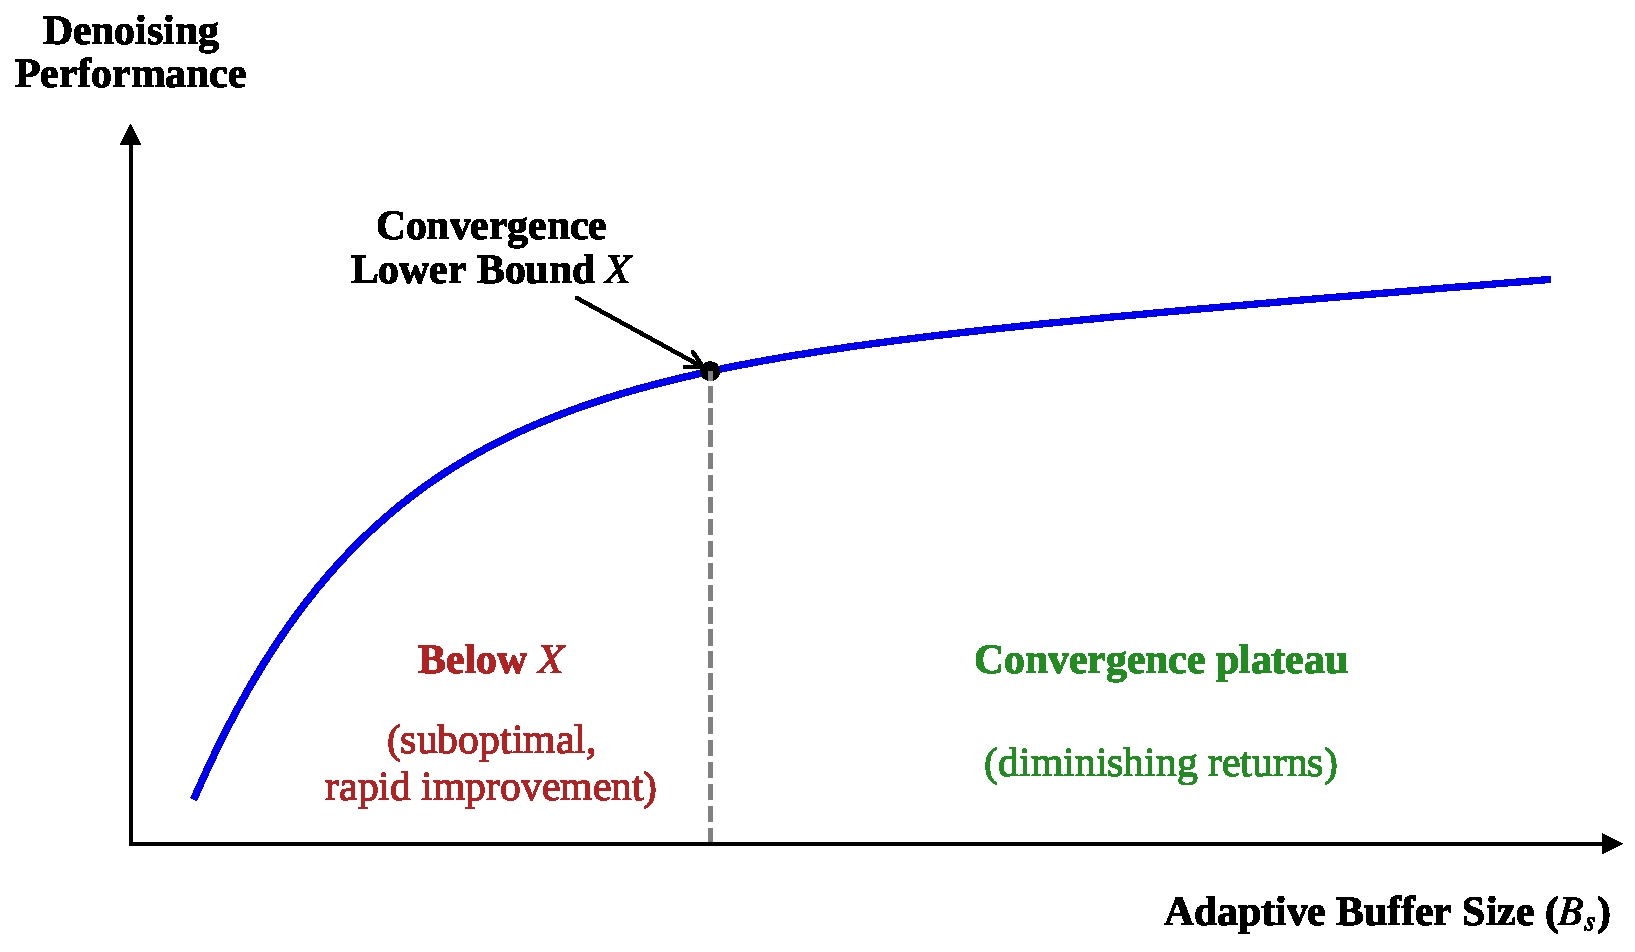
\includegraphics[width=\textwidth]{Figures/buffer_size_conceptual.pdf}
    \vspace{0.5em}
    \hrule
    \caption{Conceptual representation of the buffer size optimization problem. Performance is expected to improve as the buffer grows, then plateau in a regime of diminishing returns. The convergence lower bound $X$ marks the threshold at which this transition occurs. The empirical shape and location of this relationship are tested in Chapter~\ref{chap:results}.}
    \label{fig:bs_conceptual}
    \vspace{0.5em}
    \hrule
\end{figure}

    This research is driven by three objectives:

\begin{enumerate}
    \item Objective 1: Establish a theoretical foundation for real-time EEG denoising.

    \item Objective 2: Design and implement a systematic evaluation methodology.

    \item Objective 3: Quantify denoising performance across buffer configurations and identify the convergence threshold.
\end{enumerate}

  \section{Thesis Structure}

To systematically address the research objectives, this thesis is organized into four subsequent chapters, each serving a distinct role in the progression from theoretical foundation to empirical validation.

Chapter~\ref{chap:literature_review}, Literature Review, establishes the theoretical foundation by examining the neurophysiological origins of EEG artefacts and surveying current denoising paradigms, critically evaluating their limitations with respect to processing latency, hardware dependency, and real-time operation. It introduces the mathematical foundations relevant to time-frequency analysis and unsupervised anomaly detection, then presents the onEEGwaveLAD framework in detail, exposing the critical knowledge gap concerning its untuned hyperparameter and establishing the scientific mandate for this investigation.

Chapter~\ref{chap:methodology}, Methodology and Implementation, describes the experimental design following the CRISP-DM lifecycle. It details the dataset selection, construction of a pseudo-real-time streaming emulation, systematic parameter search strategy, configuration of baseline methods for benchmarking, formalization of performance evaluation metrics, and specification of non-parametric statistical procedures for validation, providing sufficient detail to ensure reproducibility.

Chapter~\ref{chap:results}, Results and Discussion, presents empirical findings and interprets their significance. It reports quantitative outcomes from the parameter search, identifies the convergence lower bound through multiple lines of evidence, validates findings through non-parametric testing across configurations, examines divergent metric behaviour, and assesses computational feasibility. The discussion situates findings within existing literature, interprets the mechanistic basis for observed behaviour, and acknowledges methodological limitations.

Chapter~\ref{chap:conclusion}, Conclusion, synthesizes the main contributions--the empirically determined convergence lower bound at which the framework achieves competitive performance--discusses implications for practical deployment in ecological settings, identifies study limitations, and proposes directions for future research including alternative datasets, joint hyperparameter optimization, and live streaming validation.

\chapter{Literature Review}
\label{chap:literature_review}
    
    \section{Fundamentals of EEG}
    \label{sec:fundamentals_eeg}
    
    To contextualize the evaluation of specific denoising algorithms, this section 
first outlines the physiological origins of the EEG signal and the nature of the 
interference that contaminates it. This section details the biological generation of EEG and categorizes the primary types of artefacts that necessitate advanced signal processing techniques.

        \textbf{Neurophysiological Bases of EEG.} An EEG signal is a continuous recording of the electrical activity produced by 
the brain. It primarily reflects the synchronized electrical potentials generated by large populations of neurons within the cerebral cortex~\parencite{niedermeyer2005electroencephalography}. When vast numbers of these neurons activate simultaneously, they produce a measurable electrical field. The resulting currents propagate through the brain tissue, skull, and scalp via a physical process known as ``volume conduction'', eventually reaching the surface electrodes (standardized via the International 10-20 system, as illustrated in Figure~\ref{fig:eeg_10_20})~\parencite{nunez2006electric}. Since the skull and scalp attenuate this electrical energy, the neural signals recorded at the scalp are weak, typically ranging between 10 and 100 microvolts ($\mu V$)~\parencite{buzsaki2006rhythms}. Due to this low amplitude and the energy loss during transmission, raw EEG data is susceptible to contamination from stronger internal and external electrical 
noise sources.

        \begin{figure}[!htb]
            \hrule
            \vspace{0.5em}
            \centering
            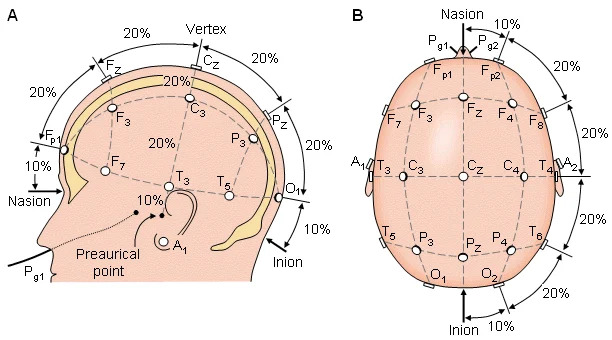
\includegraphics[width=0.50\textwidth]{Figures/the-10-20-system-with-percentages.jpg} 
            \vspace{0.5em}
            \hrule
            \caption{The International 10-20 system for EEG electrode placement on the scalp~\parencite{shriram2012eeg}}
            \label{fig:eeg_10_20}
            \vspace{0.5em}
            \hrule
        \end{figure}

        \textbf{EEG Artefacts.} In EEG signal processing, an artefact is any recorded electrical noise that does 
not originate from the targeted cortical cells~\parencite{uriguen2015eeg}. Because genuine neural signals are weak, artefacts frequently dominate the recording, masking the underlying brain activity and complicating subsequent data analysis. Artefacts are classified into two categories based on their origins: internal 
(physiological) and external (environmental)~\parencite{sweeney2012artifact}.

        \textbf{Internal (Physiological) Artefacts.} Physiological artefacts are caused by the user's own body movements outside the brain, and because these noise sources are close to the EEG sensors with relatively high electrical power, they are the hardest type of noise to remove automatically~\parencite{fatourechi2008emg}. The most common physiological noise is the Electrooculographic (EOG) artefact, which comes from eye and eyelid movements~\parencite{jiang2019removal}. Physiologically, the human eye acts like a strong dipole or small battery, with a positive front (cornea) and a negative back (retina)~\parencite{croft2000removal}. Blinking or moving the eyes changes the direction of this electrical field, creating large, slow electrical waves that mostly affect the frontal EEG channels. Consequently, EOG artefacts can be much larger than brain signals, obscuring the microvolt-level cortical activity. Electromyographic (EMG) artefacts, caused by the tightening of face, head, and neck muscles, are also disruptive~\parencite{chaddad2023electroencephalography}. Unlike the slow waves of eye movements, muscle activity creates fast, high-frequency noise. The onEEGwaveLAD framework has been specifically instantiated for real-time EMG artefact identification and mitigation~\parencite{longo2025instantiating}. EMG artefacts are especially hard to isolate because their broadband frequencies often overlap with normal high-frequency brain waves (such as Beta and Gamma bands), making it difficult to filter out the noise using standard frequency filters without accidentally deleting real brain signals~\parencite{muthukumaraswamy2013high}. Other internal noise includes Electrocardiographic (ECG) artefacts caused by the heartbeat; however, these are usually easier to predict and have a clearer periodic rhythm than eye or muscle noise~\parencite{sweeney2012artifact}. A visual comparison of these physiological contaminations against a clean neural baseline is presented in Figure~\ref{fig:wave-comparison}.

        \begin{figure}[!htb]
            \hrule\vspace{0.5em}
            \centering
            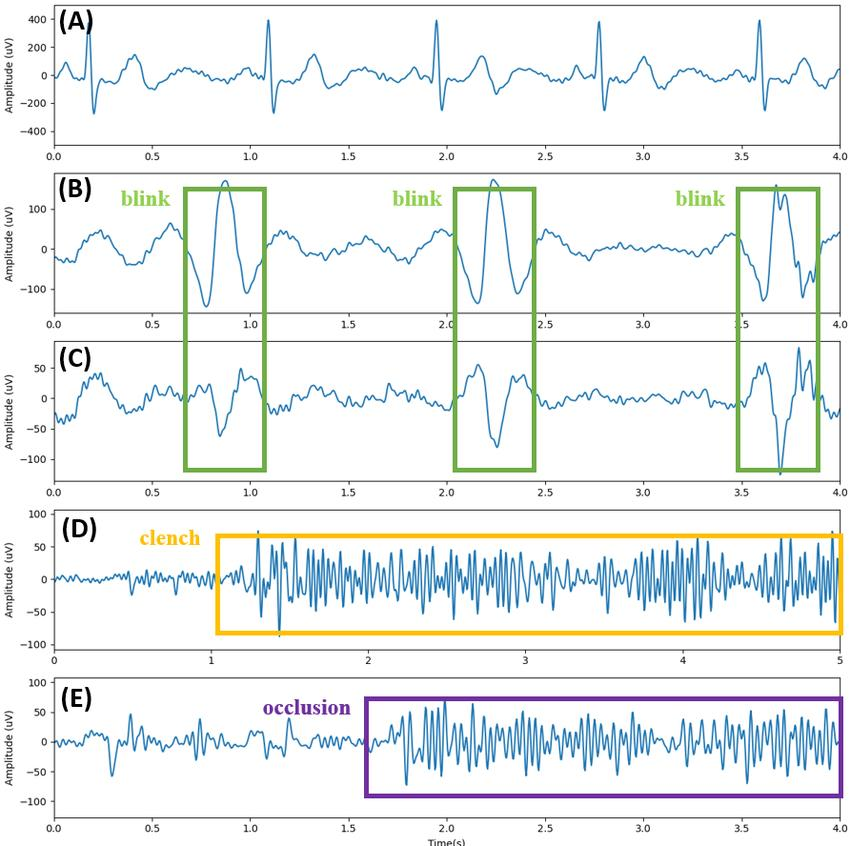
\includegraphics[width=0.85\textwidth]{Figures/wave-comparison.jpeg}
            \vspace{0.5em}\hrule
            \caption{Comparison of clean, ECG-contaminated, EOG-contaminated, and EMG-contaminated EEG waveforms~\parencite{zou2022beats}.}
            \label{fig:wave-comparison}
            \vspace{0.5em}\hrule
        \end{figure}

        \textbf{External (Extra-Physiological) Artefacts.} External artefacts come from the room environment and the hardware equipment, with the most common environmental noise being power line interference. This appears as a constant, strong wave at a fixed frequency (like 50 Hz in Europe or 60 Hz in North America) caused by the local alternating current electricity grid~\parencite{teplan2002fundamentals}. Additionally, the physical connection between the user and the hardware can create equipment noise, such as ``electrode popping'' when the impedance between the skin and the sensor suddenly changes, or general movement noise from pulling cables that can cause sharp voltage spikes~\parencite{kappenman2010impedance}. While external noise like power line interference can usually be fixed with simple notch filters or robust hardware grounding, internal physiological noise (EOG and EMG) is unpredictable and mixes with brain frequencies. The difficulty of removing these complex internal artefacts demonstrates why advanced, adaptive denoising systems like onEEGwaveLAD are needed.

            
    \section{Current Paradigms in EEG Denoising}
    \label{sec:current_paradigms}
    
    For decades, removing physiological noise has been a major challenge in EEG signal processing. Researchers have developed numerous methods to handle ECG, EOG and EMG interference; however, assessing these paradigms for modern wearable monitoring requires more than signal-to-noise ratio improvements alone. A method's true clinical and commercial usefulness depends on its processing latency, its capacity for autonomous operation, and its minimal hardware dependency~\parencite{jiang2019removal}.

        \subsection{Processing Temporality and Automaticity}
\label{subsec:processing_temporality}

Denoising algorithms are fundamentally bottlenecked by how they handle data over time. Offline processing, which remains the gold standard for clinical lab research, cleans the data only after the entire recording session is finished, enabling complex mathematical optimizations but precluding real-time applications~\parencite{uriguen2015eeg, mullen2015real}. Block-online (or pseudo-online) methods segment the continuous data stream into short, sequentially overlapping epochs (e.g., 1- to 5-second buffers). This creates an inherent latency equal to the time required to record the block plus the algorithmic computation time. While closer to real-time, performance depends on the window parameter: if the block is too short, the algorithm lacks sufficient statistical distribution to recognize the noise; if the block is too long, the data-gathering delay violates the instantaneous constraints of real-time BCI applications~\parencite{mullen2015real}. True online processing, by contrast, operates on a continuous, sample-by-sample basis or utilizes short, sliding windows (often in the millisecond range), instantly calculating and updating filtering parameters using strictly historical and current data points to achieve the near-zero latency required for modern applications.
        
Processing timing is coupled with the requirement for automaticity. Historically, noise removal relied on human neurophysiologists visually inspecting and manually discarding contaminated epochs~\parencite{uriguen2015eeg}. Modern continuous BCI systems cannot use human-in-the-loop intervention. A robust true-online system must be automated--ingesting data, isolating anomalies, and reconstructing the signal unsupervised, without manual rule-setting~\parencite{jiang2019removal}.
        
\subsection{Common Denoising Paradigms and Their Limits}
\label{subsec:common_paradigms}

The literature~\parencite{uriguen2015eeg} offers several algorithmic families for automated artefact removal, each with structural limitations under single-channel, real-time constraints. Regression-based methods and Adaptive Filtering require external reference sensors (e.g., EOG electrodes), rendering them unsuitable for minimalist headsets~\parencite{croft2000removal, sweeney2012artifact}. Blind Source Separation techniques--Principal Component Analysis (PCA) and Independent Component Analysis (ICA)--cannot separate more sources than available sensors and require computationally intensive matrix operations, disqualifying them from single-channel online deployment~\parencite{makeig1996independent, mullen2015real}. Automated pipelines (FASTER) and Artifact Subspace Reconstruction (ASR) reduce manual intervention but retain multi-channel dependencies~\parencite{nolan2010faster, chang2019evaluation}; they serve as comparison baselines in this thesis, with their parameterisation detailed in Chapter~\ref{chap:methodology}.

Single-channel methods like Empirical Mode Decomposition (EMD) suffer from mode mixing, and hybrid models (EMD-ICA, Wavelet-ICA) compound computational latency~\parencite{huang1998empirical}. Deep Learning approaches demand large pre-labeled datasets and exhibit vulnerability to concept drift when encountering novel artefacts~\parencite{zhang2021deep, craik2019deep, gama2014survey}. Traditional anomaly detectors--k-means clustering and One-Class SVM--either struggle with high-dimensional feature spaces or impose quadratic/cubic time complexity ($O(N^2)$ to $O(N^3)$), making them unscalable for continuous online processing~\parencite{scholkopf2001estimating}.

This operational void--the need for an unsupervised, single-channel anomaly detector with linear complexity--is filled by the Isolation Forest algorithm, forming the logical bridge to the onEEGwaveLAD framework~\parencite{chandola2009anomaly, longo2025oneegwavelad}. These structural limitations are amplified when considering deployment environments. Most denoising algorithms were validated in controlled laboratory settings with electrically shielded conditions and movement-restricted subjects, artificially inflating performance metrics~\parencite{mullen2015real}. Modern BCI applications demand ecological validity: ambulatory users in naturalistic environments generate non-stationary, unpredictable artefacts, while hardware constraints favor dry, single-channel headsets over dense multi-channel arrays~\parencite{jiang2019removal}. This paradigm shift justifies the integration of fast time-frequency transforms with lightweight unsupervised machine learning in frameworks like onEEGwaveLAD~\parencite{longo2025oneegwavelad}.

   \section{Wavelet Transform in EEG Signal Processing}
   \label{sec:wavelet_transform}
    
    A major limitation of the methods discussed in the previous section is that they struggle to separate short, unpredictable noise from a single data stream. Addressing this requires transforming the raw EEG data into a representation that exposes time and frequency information simultaneously. The Wavelet Transform (WT) achieves exactly this, providing the mathematical engine for modern single-channel systems like onEEGwaveLAD, whose design integrates DWT with unsupervised learning specifically for online operation~\parencite{longo2025oneegwavelad, longo2026framework}.

        \subsection{From Fourier to Wavelet Transforms}
        \label{subsec:fourier_to_wavelet}
        
        Traditionally, frequency analysis begins with the standard Fourier Transform (FT), which mathematically converts a time-domain signal into a continuous function of frequencies~\parencite{brigham1988fast}. However, because real-world signals are recorded digitally as discrete samples, computers rely on the Fast Fourier Transform (FFT). While the FFT is efficient at showing the overall frequency content of a signal, it discards temporal localization. It can calculate \textit{what} frequencies exist in a signal, but it cannot determine \textit{when} those frequencies occurred.
        
        Because EEG signals and their accompanying noise are non-stationary~\parencite{kaplan1999nonstationary}, meaning they feature sudden spikes and shifting patterns over time, looking only at the pure frequency domain is inadequate. To resolve this, the Short-Time Fourier Transform (STFT) introduces a sliding window to analyze small sections of the signal sequentially, but it is constrained by a mathematical rule known as the Heisenberg-Gabor uncertainty principle~\parencite{sejdic2009time}. In STFT, one is forced to choose a fixed window size: a short window provides good time accuracy but poor frequency resolution, whereas a long window gives precise frequency separation but blurs the timing of sudden events. This fixed resolution makes it difficult for the STFT to capture both slow EOG waves and fast EMG spikes simultaneously.

        Once the necessity of a variable-sized window is established, it is critical to distinguish between the two primary ways to compute the wavelet transform. The Continuous Wavelet Transform (CWT) slides the mother wavelet along the time axis smoothly and scales it across a broad range of sizes, creating a detailed, continuous map of the signal's frequencies over time. However, this method generates a large amount of overlapping, redundant data; because it demands heavy processing power and memory space, CWT is excellent for offline visual analysis but is unsuitable for fast, online algorithmic implementations~\parencite{addison2017illustrated}.
        
        To solve this computational bottleneck, the Discrete Wavelet Transform (DWT) discretizes the process by calculating scales and positions at specific logarithmic steps--typically using powers of two, known as dyadic scaling~\parencite{mallat1989theory}. In engineering practice, DWT is implemented using a digital filter bank where the incoming signal is recursively passed through a high-pass filter (producing Detail coefficients) and a low-pass filter (producing Approximation coefficients). Unlike CWT, this pyramidal sub-band coding method effectively minimizes data redundancy and requires significantly less computational power, inherently executing in $O(N)$ time complexity~\parencite{mallat1989theory}. The architectural evolution from standard Fourier analysis to this efficient DWT is summarized in Figure~\ref{fig:transform_evolution}. Furthermore, the multi-resolution advantage of the DWT over the rigid fixed resolution of the STFT is visually contrasted in Figure~\ref{fig:stft_vs_dwt}. 

    \begin{figure}[!htb]
    \hrule\vspace{0.5em}
    \centering
    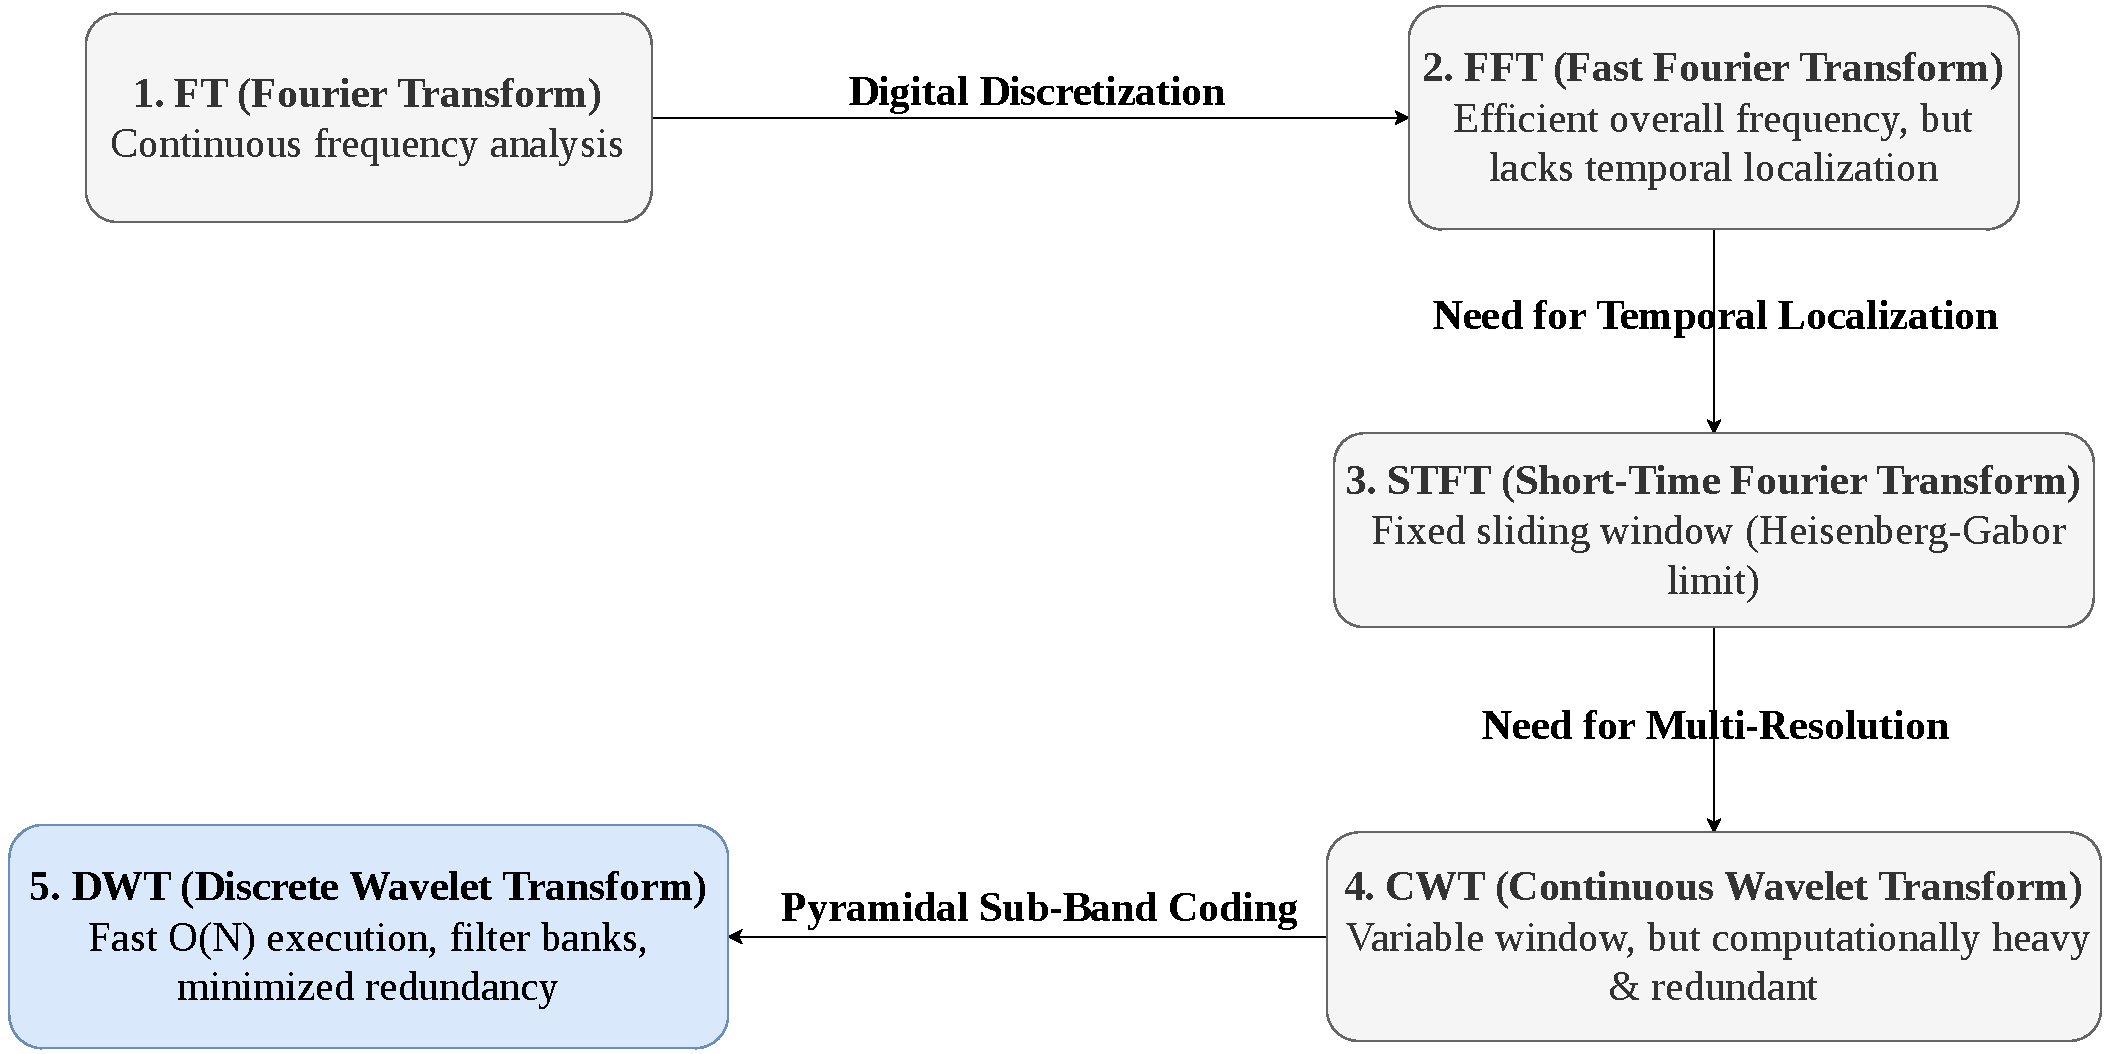
\includegraphics[width=\textwidth]{Figures/transform_evolution.pdf}
    \vspace{0.5em}\hrule
    \caption{The architectural evolution of signal processing transforms.}
    \label{fig:transform_evolution}
    \vspace{0.5em}\hrule
\end{figure}

        \begin{figure}[!htb]
        \hrule\vspace{0.5em}
            \centering
            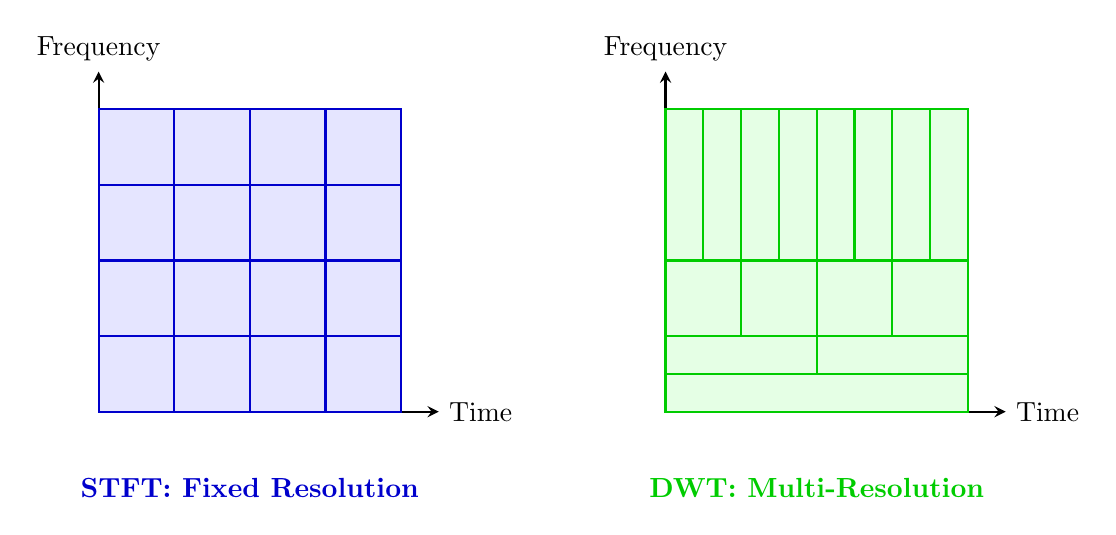
\begin{tikzpicture}[scale=1.2]
                \begin{scope}[xshift=0cm]
                    \draw[->, thick, >=stealth] (0,0) -- (3.6,0) node[right, font=\normalsize] {Time};
                    \draw[->, thick, >=stealth] (0,0) -- (0,3.6) node[above, font=\normalsize] {Frequency};
                    \foreach \x in {0, 0.8, 1.6, 2.4} {
                        \foreach \y in {0, 0.8, 1.6, 2.4} {
                            \draw[fill=blue!10, draw=blue!80!black, thick] (\x,\y) rectangle (\x+0.8, \y+0.8);
                        }
                    }
                    \node[below, font=\normalsize\bfseries, text=blue!80!black] at (1.6,-0.6) {STFT: Fixed Resolution};
                \end{scope}
                \begin{scope}[xshift=6cm]
                    \draw[->, thick, >=stealth] (0,0) -- (3.6,0) node[right, font=\normalsize] {Time};
                    \draw[->, thick, >=stealth] (0,0) -- (0,3.6) node[above, font=\normalsize] {Frequency};
                    \foreach \x in {0, 0.4, 0.8, 1.2, 1.6, 2.0, 2.4, 2.8} {
                        \draw[fill=green!10, draw=green!80!black, thick] (\x, 1.6) rectangle (\x+0.4, 3.2);
                    }
                    \foreach \x in {0, 0.8, 1.6, 2.4} {
                        \draw[fill=green!10, draw=green!80!black, thick] (\x, 0.8) rectangle (\x+0.8, 1.6);
                    }
                    \foreach \x in {0, 1.6} {
                        \draw[fill=green!10, draw=green!80!black, thick] (\x, 0.4) rectangle (\x+1.6, 0.8);
                    }
                    \draw[fill=green!10, draw=green!80!black, thick] (0, 0) rectangle (3.2, 0.4);
                    \node[below, font=\normalsize\bfseries, text=green!80!black] at (1.6,-0.6) {DWT: Multi-Resolution};
                \end{scope}
            \end{tikzpicture}
            \vspace{0.5em}\hrule
            \caption{Comparison of time-frequency resolution tiling. The STFT (left) forces a compromise between time and frequency precision. The DWT (right) utilizes a multi-resolution approach, providing time resolution for high-frequency events (like EMG spikes) and frequency resolution for low-frequency trends (like EOG waves).}
            \label{fig:stft_vs_dwt}
            \vspace{0.5em}\hrule
        \end{figure}

        \subsection{DWT Implementation and Boundary Effects}
        \label{subsec:dwt_implementation}
        
        The DWT achieves its computational efficiency through Mallat's algorithm, commonly known as the pyramidal sub-band coding scheme~\parencite{mallat1989theory}. Instead of calculating complex mathematical integrals, this algorithm processes the digital signal using a pair of complementary digital filters: a low-pass filter $h$ and a high-pass filter $g$. At each decomposition level $j$, the input signal is mathematically convolved with these filters and then downsampled by a factor of two (discarding every second data point to halve the data size), explicitly defined by the following standard equations~\parencite{mallat1989theory}, applied within the onEEGwaveLAD framework as~\parencite{longo2025oneegwavelad}:

\begin{equation}
    A_j[k] = \sum_{n} A_{j-1}[n] \cdot h[2k - n]
    \label{eq:approx_coeff}
\end{equation}

\begin{equation}
    D_j[k] = \sum_{n} A_{j-1}[n] \cdot g[2k - n]
    \label{eq:detail_coeff}
\end{equation}
        
        In these equations, $A_{j-1}$ represents the input signal entering the current level (where $A_0$ is the raw EEG signal). Equation~\ref{eq:approx_coeff} applies the low-pass filter to output the Approximation Coefficients ($A_j$), which capture the slow, low-frequency underlying trends of the brain wave, while Equation~\ref{eq:detail_coeff} applies the high-pass filter to output the Detail Coefficients ($D_j$), capturing the fast, high-frequency spikes. To build the ``pyramid,'' the high-frequency $D_j$ coefficients are stored as final outputs for that level, and only the low-frequency $A_j$ coefficients are passed down into the next level to be split again. This recursive, tree-like structure naturally divides the broad EEG spectrum into distinct clinical frequency bands (Gamma, Beta, Alpha, Theta, and Delta), allowing onEEGwaveLAD to target noise in one specific band without destroying the neural information residing in the others.
        
        While the DWT is effective, running it on a continuous, sliding-window system creates a mathematical problem known as edge effects~\parencite{torrence1998practical}. The wavelet filter requires data points on both sides of a target sample to calculate correctly, and when an algorithm processes a short, segmented block of streaming data, the filter hits a sudden boundary at the start and end of the window. This abrupt cut-off generates artificial high-frequency distortions at the edges of the processed data block. The region of the data corrupted by these boundary errors is defined as the Cone of Influence (COI)~\parencite{torrence1998practical}. To prevent downstream machine learning algorithms from confusing these mathematical errors with real physiological noise (such as an EMG spike), online systems like onEEGwaveLAD rely on continuous sliding historical buffers to manage data overlaps and mitigate boundary corruptions~\parencite{longo2025oneegwavelad}.
        
         \section{The onEEGwaveLAD Framework}
    \label{sec:oneegwavelad_framework}
    
    The time-frequency machinery established above provides only one component of a working online denoiser; it must be embedded within an architecture that also decides, without supervision, which spectral profiles correspond to artefacts. The Online EEG Wavelet-based Learning Adaptive Denoiser (onEEGwaveLAD) was developed to meet this requirement, performing pseudo-real-time sanitisation on single-channel streams while avoiding both multi-channel dependencies and the need for offline, manually labelled data~\parencite{longo2025oneegwavelad, longo2026framework}. The framework has been successfully instantiated for specific artefact types, including muscle artefact mitigation in real-time scenarios~\parencite{longo2025instantiating}. By coupling the algorithmic efficiency of the Discrete Wavelet Transform with a model-free, unsupervised anomaly detector, the framework dispenses with spatial reference sensors and predefined heuristic rules.

        \subsection{Formal Architecture and Feature Extraction}
        \label{subsec:formal_architecture}
        
        The operational blueprint of the onEEGwaveLAD framework is mathematically defined by an eight-parameter tuple~\parencite{longo2025oneegwavelad}. This configuration dictates the processing lifecycle and includes the following formal components:
        \begin{itemize}
            \item The window length ($RTW_L$) and the hardware sampling rate ($S_r$), which collaboratively define the temporal boundaries and Nyquist frequency constraints of the pseudo-real-time blocks.
            \item The designated mother wavelet (MW) used for spectral decomposition, paired with the adaptive buffer size ($B_s$) which regulates historical memory.
            \item The sub-sampling size ($IF_S$) and the total ensemble of trees ($IF_t$) required to train the isolation algorithm.
            \item The anomaly threshold ($T_a$) for isolating outliers, alongside the temporal expansion step ($E_s$) utilized during the mitigation phase.
        \end{itemize}

        The signal processing pipeline initiates by capturing a raw, univariate EEG block defined by $RTW_L$. To extract localized time-frequency features, the system executes a multi-level DWT. However, because wavelet coefficients extracted at deeper decomposition levels (representing lower frequencies) inherently possess disproportionately larger magnitudes than higher-frequency coefficients, a direct mathematical comparison would be biased. To resolve this asymmetry, the framework applies a normalization strategy, systematically dividing each coefficient by $2^m$ (where $m$ denotes the specific decomposition level) to equalize statistical variance across the spectrum~\parencite{longo2025oneegwavelad}.
        
        To synchronize the disparate temporal resolutions generated by the pyramidal sub-band coding, these normalised coefficients are systematically duplicated $2^{m-1}$ times, constructing a uniform, high-dimensional matrix known as the normalised Scaleogram. A discrete vertical slice extracted from this matrix is defined as an Instantaneous Spectral Profile (ISP). The ISP is the foundational multi-dimensional feature vector, capturing a 
detailed, localized fingerprint of the neural energy distribution at a specific 
millisecond, as depicted in Figure~\ref{fig:phase_c_scaleogram}.
        
        \begin{figure}[!htb]
            \hrule\vspace{0.5em}
            \centering
            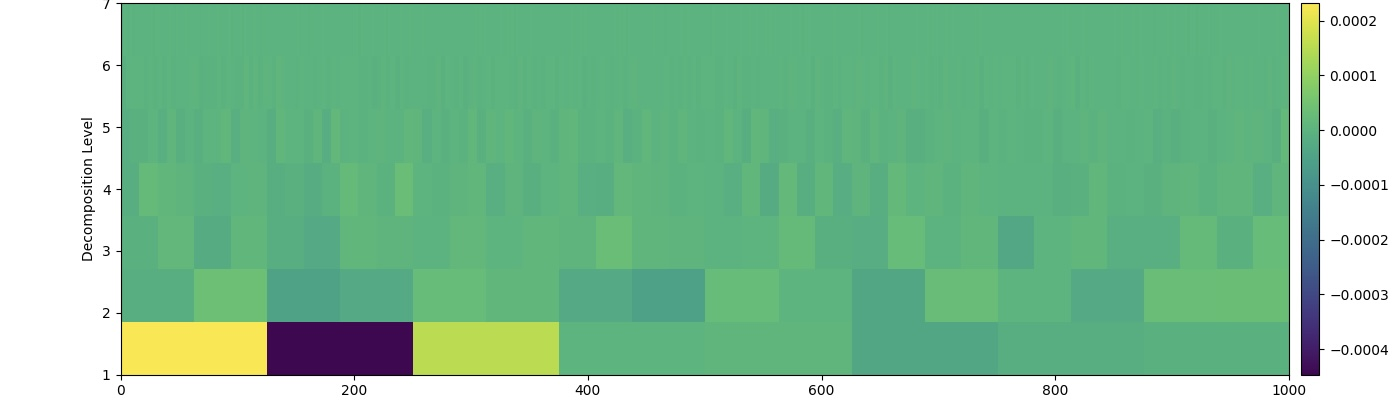
\includegraphics[width=0.9\textwidth]{Figures/phase_c_scaleogram.jpg}
            \vspace{0.5em}\hrule
            \caption{Normalised Scaleogram representing the Instantaneous Spectral Profiles (ISPs). This matrix visualizes the distribution of neural energy across different wavelet decomposition levels over a continuous temporal window~\parencite{longo2025oneegwavelad}.}
            \label{fig:phase_c_scaleogram}
            \vspace{0.5em}\hrule
        \end{figure}

        \subsection{Anomaly Detection and Signal Reconstruction}
\label{subsec:anomaly_detection_reconstruction}

Physiological artefacts appear as statistically rare Instantaneous Spectral Profiles (ISPs) compared to dense cortical rhythms, a property that the framework exploits through unsupervised anomaly detection~\parencite{longo2025oneegwavelad, longo2026framework}. The framework employs Extended Isolation Forest (eiFOREST), which constructs decision boundaries using random multidimensional hyperplanes rather than axis-parallel partitions. This enables natural isolation of anomalous ISPs in high-dimensional EEG feature spaces while maintaining linear time complexity and resilience against data swamping and masking phenomena~\parencite{hariri2019extended}. Vectors exceeding the anomaly threshold $T_a$ based on isolation path length are flagged as artefacts~\parencite{longo2025oneegwavelad}. Before executing artefact reduction, the framework discards the normalised scaleogram and retrieves the original, non-normalised DWT coefficients to ensure structural integrity during inversion. The mitigation mechanism computes the centroid of the historical buffer as the coordinate-wise mean, representing nominal brain activity. This mean serves as an inexpensive summary that can be recomputed at every window without additional distance calculations, keeping the reference compatible with online processing latency budgets. Flagged anomalies are suppressed by replacing their wavelet coefficients with values closer to this centroid, broadened temporally by the expansion parameter $E_s$ to ensure smooth transitions. Detection operates exclusively on detail coefficients; approximation coefficients ($cA$, 0-2 Hz) pass through unmodified, though the eighth detail band ($cD_8$, 2-4 Hz) capturing ocular blink energy is processed~\parencite{longo2025oneegwavelad}. The Inverse Discrete Wavelet Transform (IDWT) then recombines the retained approximation with mitigated details to yield the final denoised waveform.

        \subsection{The Hyperparameter Optimization Gap}
        \label{subsec:hyperparameter_gap}
        
        Because human neurophysiology is non-stationary, static anomaly detection models are susceptible to shifting cognitive states~\parencite{kaplan1999nonstationary}. To provide the static eiFOREST engine with necessary temporal adaptability, onEEGwaveLAD relies on a sliding historical buffer of fixed capacity, denoted as $B_s$~\parencite{longo2025oneegwavelad}. This buffer forces the algorithm to continuously retrain its isolation trees using solely the most recent sequence of ISPs, enabling the decision boundaries to dynamically track the user's evolving brain states.
        
        A fundamental assumption of this mechanism is that the sliding buffer predominantly contains genuine cortical activity rather than sustained noise, so the size of the buffer directly governs how well the detector can characterise the user's normal 
spectral profile. When the buffer is small, the eiFOREST is calibrated on a limited history and possesses insufficient baseline material to separate rare artefacts from legitimate fluctuations, which is expected to yield poorer denoising~\parencite{longo2025oneegwavelad}. As the buffer grows, the accumulated history supplies progressively richer evidence of nominal activity, and the physical expectation is that denoising quality monotonically improves and subsequently converges, with further enlargement producing diminishing returns~\parencite{gama2014survey}. Within this reformulated view, the quantity of interest is a \emph{convergence lower bound}, denoted $X$, operationally defined as the smallest buffer size beyond which the raw evaluation metrics cease to change meaningfully; below this bound the denoising quality degrades more rapidly, whereas above it the metric values settle into a regime of diminishing returns. The opposite regime, in which an oversized buffer becomes saturated with sustained artefacts and deteriorates in performance, is a theoretical edge case rather than the behaviour expected in the practical range examined here. This follows the physical expectation that larger buffers supply richer context and yield better anomaly detection without symmetric degradation. The existence and location of $X$ have not been established for the onEEGwaveLAD framework and cannot be inferred from theory alone; a conceptual representation of this reformulated relationship between buffer size and denoising performance is given in Figure~\ref{fig:bs_conceptual}, and its empirical verification through a multi-dimensional evaluation suite forms the central experimental question of this thesis. Establishing where this convergence lower bound lies cannot rest on a single signal-to-noise criterion, but depends instead on the multi-dimensional evaluation suite formalised in the following section.
        
\section{Evaluation Metrics for EEG Denoising}
\label{sec:metrics}
    
    Evaluating an EEG denoising algorithm requires balancing multiple goals: a good pipeline must remove as much artifactual noise as possible while keeping the true neural signal intact~\parencite{chen2014eeg, sweeney2012artifact}. The evaluation suite employed in this thesis follows the multi-dimensional assessment strategy advocated for online denoising frameworks~\parencite{longo2026framework} and comprises fifteen individual metrics, derived from seven core measurements: signal-to-noise ratio difference (SNR-Diff), peak signal-to-noise ratio difference (PSNR-Diff), root mean square error (RMSE), Pearson correlation coefficient (Corr), mutual information (MI), band power preservation error resolved across five frequency bands (BPPE), and magnitude squared coherence resolved across five frequency bands (MSC). Because aggressive cleaning can readily distort or destroy genuine neural rhythms, reliance on any single evaluation metric risks a misleading assessment, and a battery of complementary measures is required to capture the trade-off between artefact removal and signal preservation~\parencite{sweeney2012artifact}. To characterise how denoising quality varies across the Adaptive Buffer Size ($B_s$) and to identify the convergence lower bound $X$, the smallest buffer beyond which the raw metric values cease to change meaningfully, a multi-dimensional evaluation suite is required~\parencite{longo2025oneegwavelad}.
    
    For the mathematical formalisation of these metrics, let $N$ denote the total number of discrete samples in a given temporal window, let $y[n]$ represent the denoised signal returned by the algorithm, and let $n$ be the discrete time index ($n = 1, 2, \ldots, N$). In naturalistic single-channel recordings such as the ERP-CORE data examined in this thesis, no artefact-free counterpart of the signal exists~\parencite{longo2025oneegwavelad, kappenman2021erp}, so the reference term $x[n]$ is the original, unprocessed recording, and each metric is computed as a comparison between this raw signal and its denoised version rather than against a pristine target. This distinction is not merely notational, since the signal-to-noise measures defined below cannot depend on a clean reference and must instead operationalise the notions of signal and noise from the stimulus structure of the recording, a procedure detailed later in Section~\ref{sec:evaluation_workflow} of the methodology chapter.

        \subsection{Time-Domain Metrics}
        \label{subsec:time_domain_metrics}
        
        Time-domain metrics directly quantify the differences in energy and amplitude between the original reference signal and the processed output~\parencite{sweeney2012artifact}. Root Mean Square Error (RMSE) is standardly selected for its sensitivity to amplitude deviations and residual artifactual spikes~\parencite{longo2026framework}. It is defined as:
        \begin{equation}
            RMSE = \sqrt{\frac{1}{N} \sum_{n=1}^{N} \left(x[n] - y[n]\right)^2}
        \label{eq:rmse}
        \end{equation}
        where the squared difference between the reference and the denoised sample at each index $n$ is averaged over the entire window before extracting the square root.
        
        To evaluate the macro-level improvement in signal clarity, the Signal-to-Noise Ratio (SNR) and Peak Signal-to-Noise Ratio (PSNR) are utilized following standard definitions in EEG denoising~\parencite{chen2014eeg, longo2026framework}. They are formulated as:
        \begin{equation}
            SNR = 10 \log_{10} \left( \frac{\sum_{n=1}^{N} (x[n])^2}{\sum_{n=1}^{N} (x[n] - y[n])^2} \right)
        \label{eq:snr}
        \end{equation}
        \begin{equation}
            PSNR = 10 \log_{10} \left( \frac{(\max(x))^2}{\frac{1}{N} \sum_{n=1}^{N} (x[n] - y[n])^2} \right)
        \label{eq:psnr}
        \end{equation}
        In these formulations, the numerator of the SNR equation calculates the total energy of the original reference signal, while the denominator calculates the energy of the residual noise (the error). For PSNR, the term $\max(x)$ explicitly denotes the maximum absolute amplitude value present in the reference signal $x$, providing a peak ceiling value against which the mean squared error is compared~\parencite{chen2014eeg}. In the context of EEG artefact removal, both quantities are reported as differences relative to the unprocessed recording, $\mathrm{SNR}_{\mathrm{diff}}$ and $\mathrm{PSNR}_{\mathrm{diff}}$, yet their orientation of merit is not identical~\parencite{uriguen2015eeg}. A larger $\mathrm{SNR}_{\mathrm{diff}}$ reflects a genuine gain in the global signal-to-noise ratio and is therefore the preferable outcome, whereas for $\mathrm{PSNR}_{\mathrm{diff}}$ a smaller value denotes closer local fidelity to the original waveform and is the better result. This divergence in direction is reconciled explicitly when the metrics are combined into a common ranking, as described later in Section~\ref{sec:evaluation_workflow} of the methodology chapter.

        \subsection{Statistical and Information-Theoretic Metrics}
        \label{subsec:statistical_metrics}
        
        While time-domain metrics track energy, they cannot guarantee the structural preservation of the neural waveform. The Pearson Correlation Coefficient ($CC$) is employed to measure the linear shape matching and temporal synchrony between the filtered signal and the original reference~\parencite{chen2014eeg}:
        \begin{equation}
            CC = \frac{\sum_{n=1}^{N} (x[n] - \bar{x})(y[n] - \bar{y})}{\sqrt{\sum_{n=1}^{N} (x[n] - \bar{x})^2} \sqrt{\sum_{n=1}^{N} (y[n] - \bar{y})^2}}
        \label{eq:cc}
        \end{equation}
        where $\bar{x}$ and $\bar{y}$ represent the mean amplitude values of the respective signals across the temporal window.
        
        Furthermore, because the relationship between cortical waves and physiological noise is non-linear, Mutual Information ($MI$) is introduced based on Shannon's information theory~\parencite{cover1999elements}, applied to EEG denoising evaluation as~\parencite{longo2025oneegwavelad}. It mathematically measures the amount of core biological information shared between the two signals:
        \begin{equation}
            MI(X; Y) = \sum_{y \in Y} \sum_{x \in X} p(x,y) \log_{2} \left( \frac{p(x,y)}{p(x)p(y)} \right)
        \label{eq:mi}
        \end{equation}
        where $X$ and $Y$ represent the discrete random variables derived from the amplitude distributions of signals $x$ and $y$. The term $p(x,y)$ represents the joint probability mass function (i.e., the probability of both signals exhibiting specific amplitudes simultaneously), whereas $p(x)$ and $p(y)$ are their respective marginal probabilities. In denoising evaluation, a pronounced drop in $MI$ indicates a loss of shared information between the input and the denoised output, signalling that genuine neural structure has been discarded~\parencite{longo2025oneegwavelad}.

        \subsection{Frequency-Domain Spectral Metrics}
        \label{subsec:frequency_domain_metrics}

        Because distinct cognitive and physiological processes are tethered to specific frequency bands, a denoising operation must be assessed by how faithfully it preserves the spectral distribution of the signal rather than by amplitude criteria alone~\parencite{cohen2014analyzing}. The Band Power Preservation Error (BPPE) quantifies the relative deviation in band power between the original and denoised signals within a specified frequency range. Let $BP_x$ denote the absolute band power of the original signal, obtained through integration of the Power Spectral Density, and let $BP_y$ denote the corresponding band power of the denoised signal; the error follows as:
        \begin{equation}
            BPPE = \frac{|BP_x - BP_y|}{BP_x} \times 100\%
        \label{eq:bppe}
        \end{equation}
        The interpretation of this quantity is governed by the physiological role of the band under examination, although in every band a smaller error is preferable. In the alpha and beta ranges, which carry meaningful cortical rhythms, a small BPPE indicates that genuine neural power has survived the denoising operation, so these band-resolved errors serve as indicators of signal preservation~\parencite{cohen2014analyzing}. In the delta and theta ranges, frequently corrupted by ocular activity~\parencite{croft2000removal}, and in the gamma range, subject to muscular contamination~\parencite{muthukumaraswamy2013high}, the same low-error criterion is retained, but the resulting figures are grouped with the artefact-oriented family, following the polarity convention defined for the framework~\parencite{longo2025oneegwavelad}.

        Magnitude Squared Coherence (MSC) complements this spectral view by measuring the frequency-resolved consistency between the original and denoised signals rather than a difference in power~\parencite{sweeney2012artifact}:
        \begin{equation}
            MSC(f) = \frac{|P_{xy}(f)|^2}{P_{xx}(f)P_{yy}(f)}
        \label{eq:msc}
        \end{equation}
        where $f$ denotes the frequency bin under evaluation, $P_{xy}(f)$ is the cross-spectral density between the original and denoised signals, and $P_{xx}(f)$ and $P_{yy}(f)$ are their respective auto-spectral densities. Computing the coherence over a single continuous block evaluates to unity across all frequencies, so Welch's method of overlapping, averaged segments is required to obtain a meaningful estimate~\parencite{sweeney2012artifact}; within a short online window, however, dividing the signal into shorter overlapping segments reduces the frequency resolution ($\Delta f = S_r / N_{seg}$), an unavoidable trade-off that must be managed when narrow bands such as alpha ($8$--$12$ Hz) are examined. As with the band power error, the coherence is read according to the role of each band: a high coherence in the alpha and beta ranges reflects the retention of cortical rhythms and is preferred, whereas in the ocular- and muscle-dominated bands a reduced coherence with the raw signal is preferred, since it reflects successful attenuation of the contaminating activity~\parencite{longo2025oneegwavelad}.

        Taken together, the band-dependent behaviour of the two spectral metrics establishes that no single frequency-domain figure can summarise denoising quality on its own, since the same operation that is beneficial in one band may be detrimental in another, and the merit of a given change is decided by whether the band predominantly carries neural information or contamination. This observation motivates the organisation of the full metric suite into two complementary groups according to their functional role: one concerned with the preservation of genuine neural content and one with the suppression of artefacts~\parencite{sweeney2012artifact, longo2026framework}. A complete summary of these evaluation metrics and their respective analytical objectives is provided in Table~\ref{tab:evaluation_metrics}.

It is important to note that this functional classification--distinguishing metrics by whether they assess signal preservation or artefact mitigation--reflects conventional evaluation practice and is independent of the behavioural classification that emerges from the empirical analysis in subsequent chapters. The latter classification groups metrics according to their response characteristics as the Adaptive Buffer Size varies: a majority of ten metrics exhibit monotonic convergence behaviour (the similarity-preservation camp), while five metrics (SNR-Diff and PSNR-Diff) exhibit non-monotonic behaviour at large buffer sizes (the artefact-removal camp). This behavioural taxonomy, which reflects the empirical findings of this thesis rather than conventional functional categorization, is introduced in Chapter~\ref{chap:methodology} and detailed in Chapter~\ref{chap:results}.
        
\begin{table}[!htb]
    \centering
    \renewcommand{\arraystretch}{1.3}
    \begin{tabularx}{\textwidth}{@{} l c >{\raggedright\arraybackslash}X >{\raggedright\arraybackslash}X @{}}
    \toprule
    \textbf{Metric (acronym)} & \textbf{Eq.} & \textbf{Evaluative role} & \textbf{Orientation of merit} \\
    \midrule
    SNR difference (SNR-Diff)      & \ref{eq:snr}  & Signal preservation & Higher is better \\
    PSNR difference (PSNR-Diff)    & \ref{eq:psnr} & Artefact mitigation & Lower is better \\
    Root mean square error (RMSE)  & \ref{eq:rmse} & Artefact mitigation & Lower is better \\
    Pearson correlation (CC)       & \ref{eq:cc}   & Signal preservation & Higher is better \\
    Mutual information (MI)        & \ref{eq:mi}   & Signal preservation & Higher is better \\
    BPPE, alpha / beta             & \ref{eq:bppe} & Signal preservation & Lower is better \\
    BPPE, delta / theta / gamma    & \ref{eq:bppe} & Artefact mitigation & Lower is better \\
    MSC, alpha / beta              & \ref{eq:msc}  & Signal preservation & Higher is better \\
    MSC, delta / theta / gamma     & \ref{eq:msc}  & Artefact mitigation & Lower is better \\
    \bottomrule
    \end{tabularx}
    \caption{Evaluation metrics grouped by their functional role in denoising assessment, with the equation defining each metric and its orientation of merit. The spectral metrics are resolved per frequency band, so that the same quantity serves signal preservation in the neural bands and artefact mitigation in the contaminated bands. The behavioural classification of these metrics according to their convergence characteristics as buffer size varies is introduced in Chapter~\ref{chap:methodology} and analysed in Chapter~\ref{chap:results}. This multi-dimensional evaluation suite follows the framework established by~\parencite{longo2026framework} and applied in~\parencite{longo2025oneegwavelad}.}
    \label{tab:evaluation_metrics}
\end{table}

        
    \section{Chapter Summary and Identified Gaps}
    \label{sec:chapter_summary_gaps}
    
    This chapter has established the theoretical foundation necessary for real-time EEG denoising in single-channel, ecological settings. The review of current paradigms demonstrated that traditional techniques--such as Independent Component Analysis (ICA) and Adaptive Filtering (AF)--are constrained by multi-channel dependencies, computational bottlenecks, or the requirement for external reference sensors. The combination of the Discrete Wavelet Transform (DWT) and unsupervised anomaly detection, as instantiated in the onEEGwaveLAD framework, addresses these architectural limitations by operating on univariate streams without spatial reference or manual calibration~\parencite{longo2025oneegwavelad}. However, this literature review also highlights a critical operational gap: while onEEGwaveLAD resolves the architectural bottlenecks of previous methods~\parencite{longo2026framework}, its reliance on the Extended Isolation Forest (eiFOREST) introduces a dependence on temporal context that has not been empirically characterized. Specifically, the influence of the Adaptive Buffer Size ($B_s$) on denoising quality remains untested. A buffer that is too small leaves the detector with insufficient historical context to characterise normal activity, an effect that is expected to manifest as faster degradation at the lower end of the buffer range. The precise location of the convergence lower bound $X$, beyond which raw metric values cease to change meaningfully, has not been determined for real-time EEG processing. While the framework's architecture and individual components are detailed in the originating study~\parencite{longo2025oneegwavelad} and the comprehensive theoretical foundation is established in the doctoral thesis~\parencite{longo2026framework}, the optimization of the buffer size parameter remains an open empirical question that this research addresses through systematic grid search and multi-criteria convergence analysis.
    
    This identified gap leads to the central research question of this thesis: \textit{At which Adaptive Buffer Size does the onEEGwaveLAD framework exhibit convergence in denoising performance, such that further increases in buffer depth yield only diminishing returns, and does this convergence threshold correspond to a level of performance that reaches or exceeds established baseline methods?} The question decomposes into two complementary concerns: first, locating the convergence lower bound $X$ at which the framework's internal metrics stabilise; and second, establishing whether the performance attained at $X$ is competitive with automated alternatives such as FASTER and Artefact Subspace Reconstruction (ASR).
    
    Answering this research question requires the empirical methodology developed in Chapter~\ref{chap:methodology}, whose design follows directly from the theoretical requirements identified above. The experimental strategy addresses four design imperatives that emerge from the literature gaps:
    
    \begin{enumerate}
        \item \textbf{Isolation of the independent variable.} Because the research question targets a single hyperparameter, the empirical design fixes every element of the onEEGwaveLAD framework except $B_s$, so that observed variation in denoising quality can be attributed to buffer depth rather than to confounded factors (Section~\ref{sec:modeling_instantiation}).
        
        \item \textbf{Multi-dimensional evaluation.} Locating the convergence lower bound demands more than conventional signal-to-noise calculations, since a single metric can be misleading. The evaluation employs fifteen complementary metrics spanning time-domain, statistical and frequency-domain perspectives (Section~\ref{sec:metrics}), organised into similarity-preservation and artefact-removal categories to capture the trade-off between waveform fidelity and contamination suppression.
        
        \item \textbf{External benchmarking.} Establishing whether performance at $X$ is competitive requires comparison against established methods under identical conditions. The design compares onEEGwaveLAD against FASTER and four ASR variants within a 
unified non-parametric ranking framework, where the seven buffer configurations 
and five baselines are treated as twelve methods subjected to joint Friedman and 
Nemenyi analysis (Section~\ref{sec:evaluation_workflow}).
        
        \item \textbf{Two-stage grid search.} The unknown location of $X$ necessitates a coarse-to-fine exploration strategy. The empirical design employs a logarithmic coarse grid ($B_s \in \{1, 2, 4, 8, 16, 32, 64\}$) to identify the approximate convergence region, followed by a linear refined grid ($B_s \in \{4, 6, 8, 10, 12, 14, 16, 18\}$) to precisely locate the lower bound within that region (Section~\ref{subsec:design_grid_search}).
    \end{enumerate}
    
\chapter{Methodology and Implementation}
\label{chap:methodology}
 
\section{Research Understanding and Hypothesis Formulation}
 
The move from the literature review to empirical work requires a methodological structure that aligns the experimental design with the gaps identified earlier. This research follows the Cross-Industry Standard Process for Data Mining (CRISP-DM) lifecycle, whose opening phase concerns research understanding: the translation of high-level objectives into precise, testable statements before any data is manipulated~\parencite{wirth2000crisp}. Applied to the present study, this phase targets a specific property of the Extended Isolation Forest used within onEEGwaveLAD, namely its dependence on the recent history supplied through the sliding buffer when it operates on non-stationary EEG~\parencite{longo2025oneegwavelad}. Understanding how the algorithm consumes this historical context allows the design of later phases to isolate and measure the effect of the buffer size rather than merely observe it.

\subsection{Translation of Literature Gaps into a Technical Hypothesis}
\label{subsec:literature_gaps_hypotheses}
 
As set out in the literature review, onEEGwaveLAD accommodates the non-stationarity of EEG by retraining its isolation trees on a sliding buffer of recent Instantaneous Spectral Profiles, whose depth is fixed by the Adaptive Buffer Size ($B_s$)~\parencite{longo2025oneegwavelad}. The value of this parameter governs how much recent history the detector can draw upon when it establishes what constitutes nominal activity. Understanding how the algorithm consumes this historical context allows the design of later phases to isolate and measure the effect of the buffer size rather than merely observe it. The engineering question is therefore at which buffer depth the framework first attains this converged level of performance.
 
Accordingly, the investigation is framed around a lower bound on the buffer size and is anchored by the following hypothesis:
 
\begin{itemize}
  \item \textbf{Research hypothesis:} If the Adaptive Buffer Size ($B_s$) is systematically increased across a two-stage grid search, then denoising performance will improve monotonically until a convergence lower bound $X$ is reached, beyond which further increases yield diminishing returns, and at which 
the framework attains competitive performance relative to established baseline methods.
\end{itemize}

The convergence lower bound $X$ is defined operationally as the smallest buffer size beyond which the raw metric values cease to change meaningfully, assessed through three complementary criteria: a parameter-free elbow-detection algorithm applied to normalised marginal improvement curves, a rank-based threshold within the Nemenyi critical difference framework, and a robustness check via median aggregation, as detailed in Section~\ref{subsec:convergence_lower_bound}. This operational definition connects the convergence behaviour observed in the metric trajectories with the statistical significance established by the rank-based tests.

Testing this hypothesis requires a pseudo-real-time streaming emulation that reproduces continuous, causal data arrival while recording the algorithm's output across the fifteen complementary metrics, so that any significant effect can be attributed to $B_s$ rather than to confounded factors. The comparison evaluates the framework against five automated baseline methods under identical preprocessing and evaluation conditions, so the behaviour across buffer sizes is judged relative to recognised alternatives rather than in isolation. The experimental design separates the variables into independent ($B_s$), dependent (fifteen denoising metrics), and controlled (all other framework parameters) categories, with their formal instantiation detailed in Section~\ref{sec:modeling_instantiation}. Figure~\ref{fig:methodology_overview} provides a comprehensive overview of the experimental design, illustrating the progression from the research hypothesis through the four CRISP-DM phases and the three-tier evaluation strategy to the multi-criteria convergence identification protocol.

\begin{figure}[!htb]
\hrule\vspace{0.5em}
    \centering
    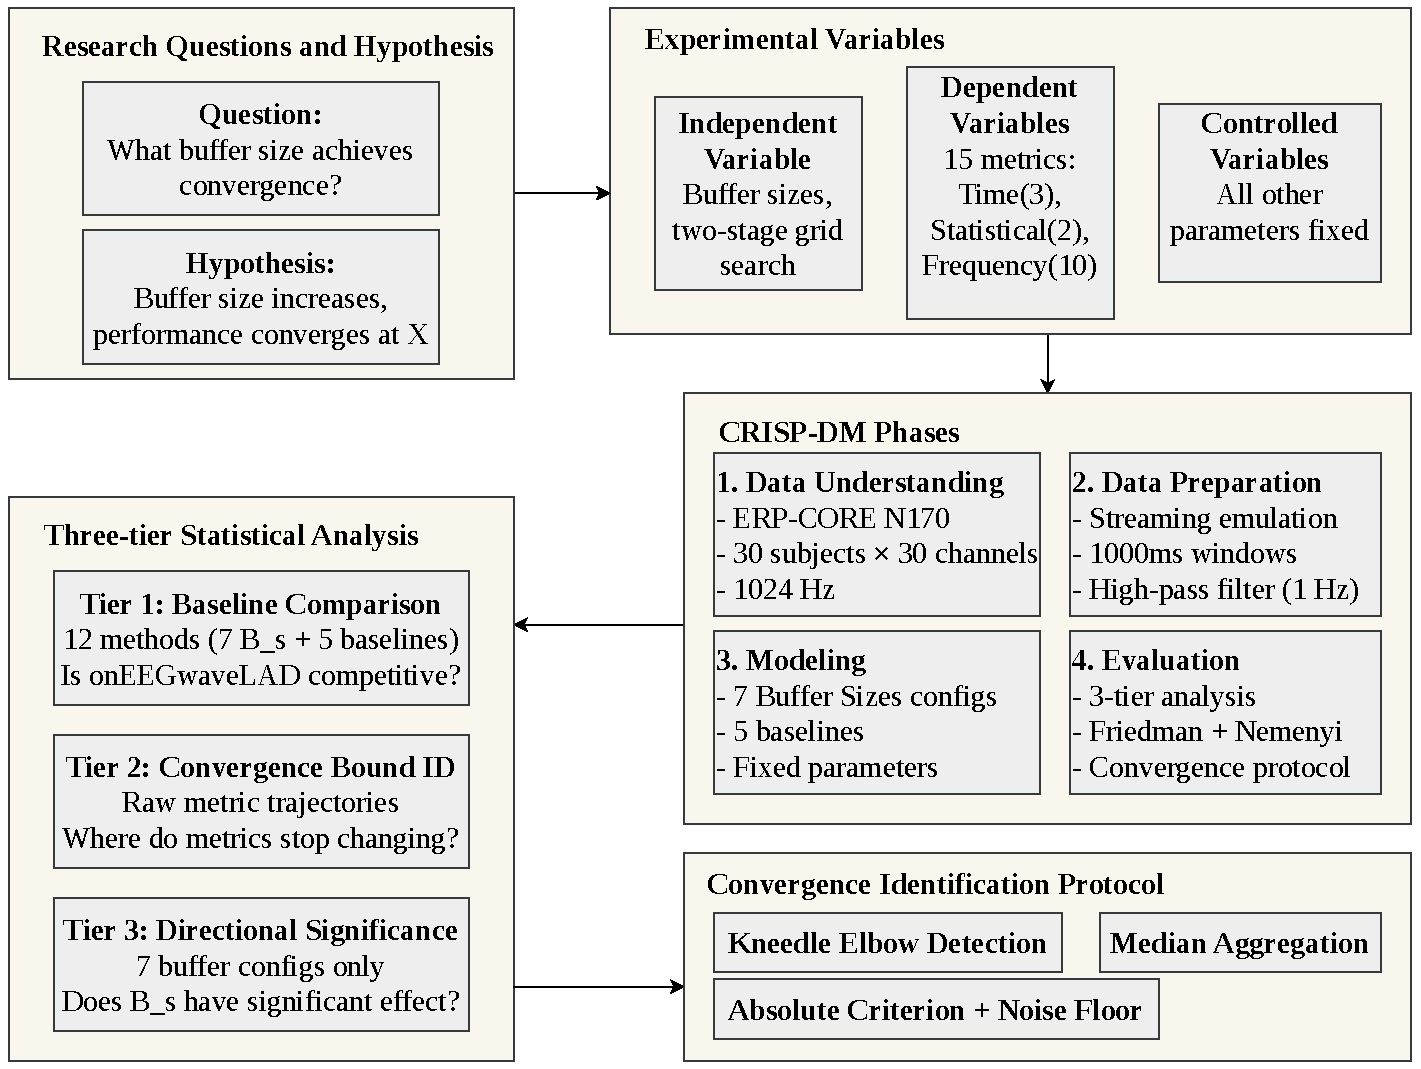
\includegraphics[width=\textwidth]{Figures/methodology_overview.pdf}
    \vspace{0.5em}\hrule
    \caption{Overview of the experimental design and methodology (Chapter~\ref{chap:methodology}).}
    \label{fig:methodology_overview}
    \vspace{0.5em}\hrule
\end{figure}

\section{Data Understanding and Experimental Setup}
 
The empirical validation of the onEEGwaveLAD framework requires a standardised, openly available EEG corpus containing both well-defined neural responses and a realistic level of physiological contamination. This study uses the Event-Related Potentials Open Resource(ERP-CORE), a dataset assembled for reproducible ERP research and distributed with documented recording and processing procedures~\parencite{kappenman2021erp}. Among its paradigms, the N170 face-processing task was retained, since it elicits a reliable occipito-temporal response while its continuous recordings retain frequent ocular activity, chiefly blinks and saccades, in the frontal channels. This pairing of a recoverable neural target with naturally occurring artefacts provides a demanding yet controlled setting for observing the anomaly-detection behaviour of the Extended Isolation Forest. The full cohort of thirty subjects was evaluated, so the reported behaviour reflects inter-subject variability rather than a single favourable recording. This sample size, representing the entire N170 paradigm subset of the ERP-CORE dataset, provides sufficient statistical power for the non-parametric tests described in Section~\ref{sec:evaluation_workflow}. The thirty-channel dense array yields $30 \times 30 = 900$ independent channel--subject observations per buffer configuration in the pooled analyses.
 
The recordings were used in their temporally aligned form, identified by the \texttt{shifted\allowbreak .set} suffix and stored in the EEGLAB format~\parencite{delorme2004eeglab}. These files were chosen because their event markers and continuous samples preserve the correspondence between stimulus onsets and the ongoing signal, a property later required by the event-based signal-to-noise computation described in Section~\ref{sec:evaluation_workflow}. Ingestion was carried out with MNE-Python, an open-source library for electrophysiological data~\parencite{gramfort2013meg}, from which the native sampling frequency of $1024$~Hz was read and retained as the reference value for the windowing and wavelet calculations that follow. Preserving this native rate, rather than resampling, keeps the temporal granularity of the stream consistent with the acquisition hardware that a real deployment would rely on.
 
A thirty-channel array was configured according to the International 10--20 system, with electrode coordinates mapped through the standard 10-5 template (\ {standard-10-5-cap385.elp}) to ensure consistent topographical placement~\parencite{oostenveld2001five}. The selected electrodes span the frontal (for example Fp1, Fp2, Fz), central (C3, C4, Cz), parietal (P3, P4, Pz) and occipito-temporal (O1, O2, PO7, PO8) regions, giving broad coverage across functionally distinct scalp zones. Although onEEGwaveLAD operates on one channel at a time and does not exploit spatial cross-covariance~\parencite{longo2025oneegwavelad}, processing this dense array channel by channel exposes the framework to artefact signatures that differ markedly between regions, from large ocular deflections at frontal sites to lower-amplitude activity over posterior areas. Evaluating every channel under a single fixed parameter set therefore tests whether the framework generalises across scalp locations without per-channel manual tuning, though the findings remain bounded to the electrode density and placement scheme employed here.
    
Alongside the thirty scalp electrodes, each recording provides three electrooculographic channels, namely the left and right horizontal derivations (HEOG\_left, HEOG\_\allowbreak right) and the lower vertical derivation (VEOG\_lower). These channels are not denoised or evaluated as neural signals; the vertical derivation is used by one of the baseline methods to identify ocular components, as described in Section~\ref{sec:baseline_methods}, and all three are separated from the scalp channels before the average re-referencing step so that ocular activity does not propagate into the common reference. The complete channel complement and acquisition
configuration are summarised in Table~\ref{tab:dataset_spec}.

\begin{table}[!htb]
        \centering
        \renewcommand{\arraystretch}{1.3}
        \resizebox{0.80\textwidth}{!}{%
        \begin{tabular}{@{} l l @{}}
        \toprule
        \textbf{Configuration Parameter} & \textbf{Specification} \\ 
        \midrule
        \textbf{Dataset Repository} & ERP-CORE (Event-Related Potentials Open Resource) \\ 
        \textbf{Experimental Paradigm} & N170 (Visual Face Processing) \\ 
        \textbf{Ingestion Format} & EEGLAB format (`.set` / shifted continuous data) \\ 
        \textbf{Sampling Frequency ($S_r$)} & 1024 Hz \\ 
        \textbf{Channel Topology} & 30 Channels (Standard 10-5 Cap Mapping) \\ 
        \textbf{Evaluated Subjects} & Subjects 1 to 30 (Full Evaluation Cohort) \\ 
        \textbf{Data Ingestion Engine} & MNE-Python Library \\ 
        \bottomrule
        \end{tabular}%
        }
        \caption{Technical specifications of the dataset and sensor montage utilized for the streaming emulation.}
        \label{tab:dataset_spec}
    \end{table}
    
    To illustrate the nature of the contamination present in the ERP-CORE recordings, Figure~\ref{fig:raw_eeg_traces} displays representative raw EEG signals from a single subject across seven channels spanning frontal to occipital regions. The frontal channels (Fp1, Fp2) exhibit frequent high-amplitude deflections exceeding $\pm 100~\mu$V, characteristic of ocular artefacts, while posterior channels (O1, O2) display comparatively clean activity with amplitudes typically below $\pm 30~\mu$V. This heterogeneity across the scalp motivates the single-channel, channel-by-channel denoising strategy employed by onEEGwaveLAD.

\begin{figure}[!htb]
\hrule\vspace{0.5em}
    \centering
    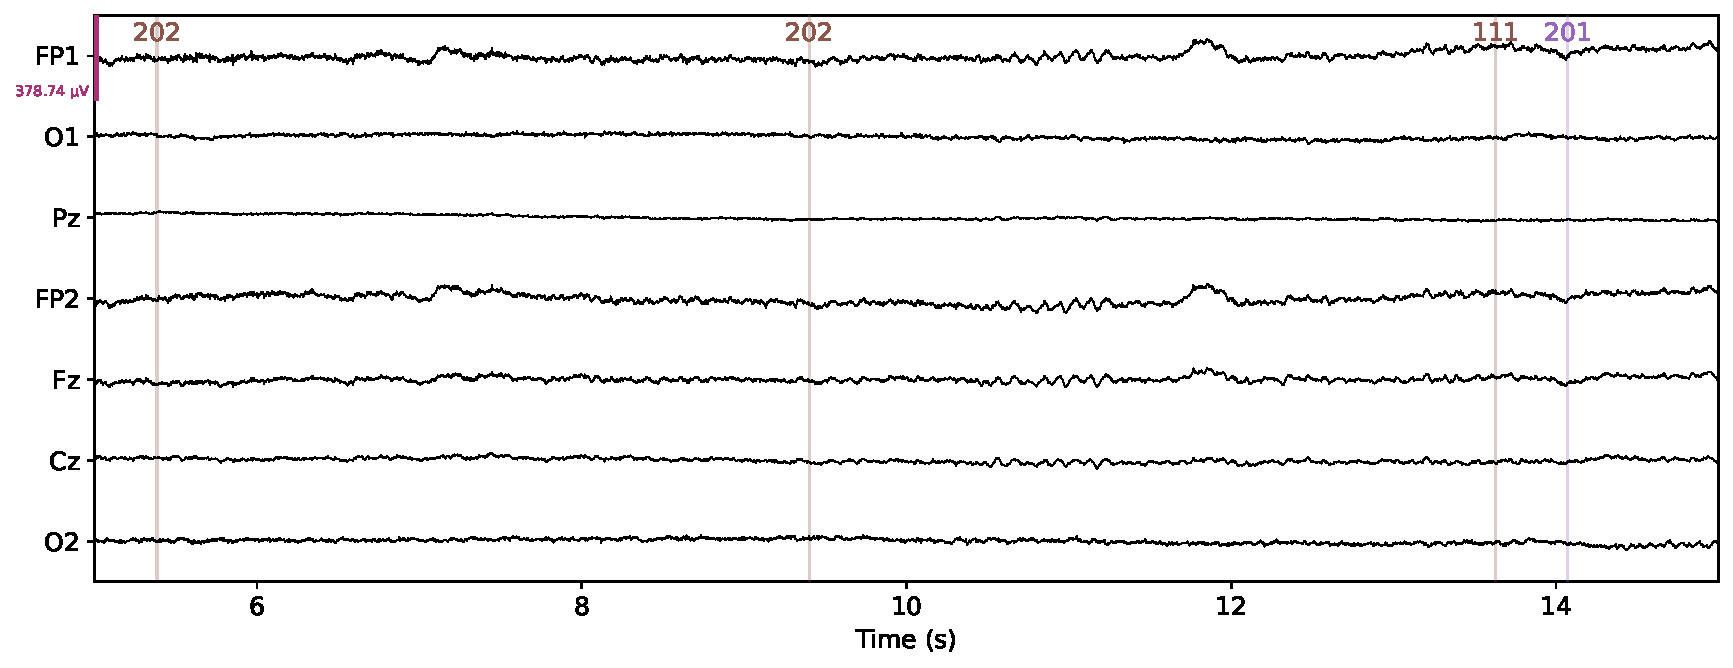
\includegraphics[width=0.95\textwidth]{Figures/raw_eeg_traces.pdf}
    \vspace{0.5em}\hrule
    \caption{Representative raw EEG signals from the ERP-CORE N170 dataset (Subject 1, 5-15 seconds). Seven channels spanning frontal (Fp1, Fp2), central (Fz, Cz, Pz), and occipital (O1, O2) regions illustrate the heterogeneous contamination profile. Red boxes mark ocular artefacts; stimulus onsets are indicated by vertical dashed lines. Note the amplitude gradient: frontal channels exhibit deflections exceeding $\pm 100~\mu$V, while posterior channels remain below $\pm 30~\mu$V.}
    \label{fig:raw_eeg_traces}
    \vspace{0.5em}\hrule
\end{figure}

\section{Data Preparation, Unified Preprocessing, and Streaming Emulation}
\label{sec:data_prep_streaming}

Because the selected ERP-CORE recordings are stored as a continuous offline signal, they must be reorganised into a sequential stream before the pseudo-real-time behaviour of the onEEGwaveLAD pipeline can be assessed~\parencite{longo2025oneegwavelad}. The recordings are real and unmodified; what is emulated is the block-by-block, causally constrained processing mode of a live acquisition system, ensuring that each denoising decision uses only current and strictly past samples. To avoid loading each full multichannel recording into memory at once, a Python generator traverses the ingested signal and extracts and yields one temporal block at a time. This iterative yielding reproduces the chronological, block-by-block arrival of samples that a live Brain-Computer Interface would receive, and it constrains the anomaly detector to current and strictly past samples, with no access to future data at the moment a window is processed.

The temporal length of each block follows the Real-Time Window Length ($RTW_L$) of the onEEGwaveLAD framework~\parencite{longo2025oneegwavelad}, set here to a baseline of $1000$~milliseconds. For the sub-band coding scheme of the Discrete Wavelet Transform to downsample symmetrically across successive decomposition levels, the number of samples in a block must be a power of two; a non-dyadic length would otherwise require zero-padding or an asymmetric boundary extension, either of which injects spurious high-frequency content into the sub-bands~\parencite{mallat1989theory}. The pipeline therefore computes the number of samples implied by the target window and the sampling rate and rounds it up to the nearest power of two via a logarithmic ceiling, adjusting the operational window length to match. At the $1024$~Hz sampling rate of the ERP-CORE recordings, a $1000$~millisecond window corresponds to exactly $1024 = 2^{10}$ samples, so this block already satisfies the dyadic-length requirement and the adjustment reduces to an identity in the present configuration; the rounding step is retained so that the same streaming logic remains valid for acquisition hardware operating at other
sampling rates.

Using this block length as a fixed step, the generator slices the raw continuous signal across all thirty selected channels in sequence, without overlap between successive windows. Each extracted window is packaged together with its start and end sample indices and the corresponding raw temporal segment, ready for wavelet decomposition. This arrangement supplies the isolation engine with a chronologically ordered stream in which each window is decomposed, scored and reconstructed before the next is drawn.

Before the windowed stream reaches the denoising stage, and in order to keep the comparison with the baseline methods on identical terms, a common preprocessing convention is applied that follows the procedure established for the framework~\parencite{longo2025oneegwavelad, longo2026framework}. The scalp signal is first high-pass filtered at $1$~Hz to remove slow drift below the band of interest, a standard operation applied uniformly to every buffer configuration and therefore neutral with respect to the effect under study. Crucially, average re-referencing is not applied to the input of onEEGwaveLAD; instead, each of the thirty channels is denoised independently on its high-pass-filtered signal, and the average reference is computed only afterwards, over the thirty denoised outputs. This ordering is adopted for two reasons. First, applying the average reference before denoising would propagate contamination from heavily artefactual channels (e.g., frontal electrodes dominated by ocular activity) into the reference itself, thereby distributing that contamination across all channels and complicating the subsequent anomaly detection~\parencite{yao2005comparative}. By deferring re-referencing until after single-channel denoising, each channel is cleaned in isolation, so that the average reference computed from the denoised signals reflects predominantly neural activity rather than shared artefacts. Second, this deferred re-referencing preserves the single-channel independence that the onEEGwaveLAD framework requires, since the framework operates on univariate streams without exploiting spatial covariance~\parencite{longo2025oneegwavelad}. During the average re-referencing operation, a flat channel--a synthetic channel with constant zero amplitude--is added to the thirty denoised EEG channels before computing the mean, following the procedure documented in~\textcite{miyakoshi_makoto_pipeline} and theoretically justified by~\textcite{bertrand1985theoretical}. This augmentation is necessary to prevent rank deficiency in the re-referenced montage: without the flat channel, the average reference imposes a linear constraint (the sum of all re-referenced signals is exactly zero at every sample), reducing the effective degrees of freedom and distorting subsequent statistical comparisons~\parencite{bigdely2015prep}. The addition of the flat channel restores full rank to the montage while preserving the desired common-mode rejection property of the average reference~\parencite{nunez2006electric}. The reference against which the denoised output is later assessed is likewise the average-re-referenced version of the high-pass-filtered recording, constructed with an identical flat-channel augmentation, so that the input and output references are directly comparable. This preprocessing order--single-channel denoising followed by average re-referencing with flat-channel augmentation--reproduces exactly the procedure used for the baseline methods in Section~\ref{sec:baseline_methods} and makes the subsequent ranking a fair comparison. Figure~\ref{fig:preprocessing_pipeline} illustrates the complete data flow from raw acquisition to the final average-re-referenced output.

\begin{figure}[!htb]
\hrule\vspace{0.5em}
    \centering
    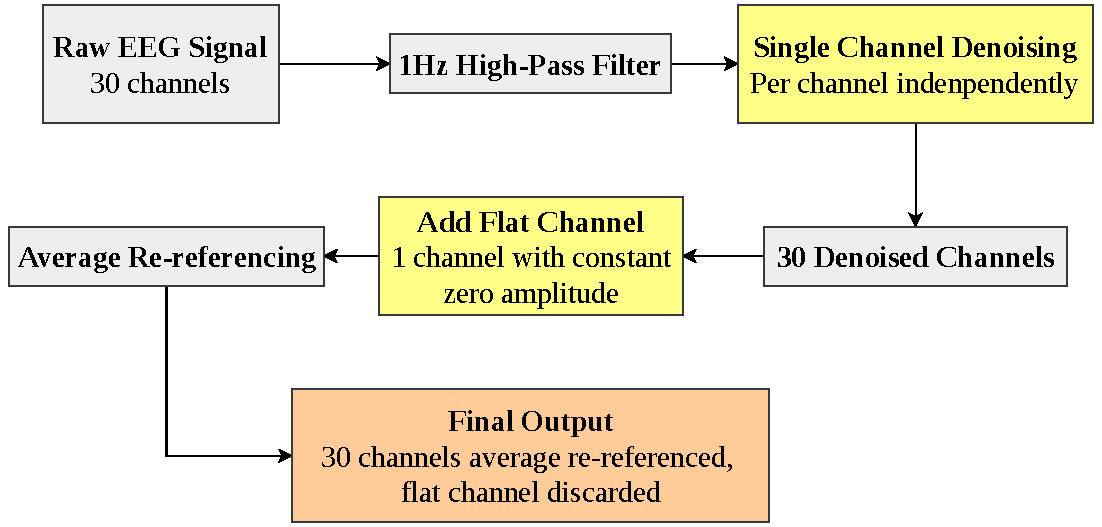
\includegraphics[width=\textwidth]{Figures/preprocessing_pipeline.pdf}
    \vspace{0.5em}\hrule
    \caption{Preprocessing pipeline showing the sequence from raw EEG through single-channel denoising to average re-referencing. Each of the thirty channels is denoised independently on its high-pass-filtered signal to prevent artefact propagation through the reference (justification detailed in text). A flat channel is added before computing the average reference to prevent rank deficiency, following~\textcite{miyakoshi_makoto_pipeline} and justified by~\textcite{bertrand1985theoretical} and~\textcite{bigdely2015prep}. The flat channel is discarded after re-referencing, yielding the final thirty-channel output used for evaluation.}
    \label{fig:preprocessing_pipeline}
    \vspace{0.5em}\hrule
\end{figure}

This ordering--single-channel denoising followed by average re-referencing with flat-channel augmentation--reproduces exactly the procedure used for the baseline methods in Section~\ref{sec:baseline_methods} and is what makes the subsequent ranking a fair comparison.

\section{Modeling: The onEEGwaveLAD Pipeline Instantiation}
\label{sec:modeling_instantiation}
 
Having established the streaming environment, the modelling phase fixes every element of the onEEGwaveLAD pipeline except the parameter under study, so that any change in denoising behaviour can be attributed to the Adaptive Buffer Size alone. The framework is defined by an eight-parameter tuple~\parencite{longo2025oneegwavelad}; this section states the value assigned to each component, the engineering reasons behind those choices, and the way the buffer size is
varied across the grid search.

Figure~\ref{fig:oneegwavelad_pipeline_focus} illustrates the seven-phase architecture of the framework, with Phase D--the Adaptive Buffer Size mechanism that feeds historical context into the Extended Isolation Forest--highlighted in red to mark the exclusive focus of this thesis. The complete parameter instantiation, including the independent variable ($B_s$), comparison methods, dependent variables (the fifteen evaluation metrics), and all controlled variables, is summarised in Table~\ref{tab:instantiation}. The following subsections describe how each stage was configured in code, focusing on the parameters passed to each component and their practical motivation. Mathematical derivations are in Chapter~\ref{chap:literature_review}.

\begin{figure}[!htb]
\hrule\vspace{0.5em}
    \centering
    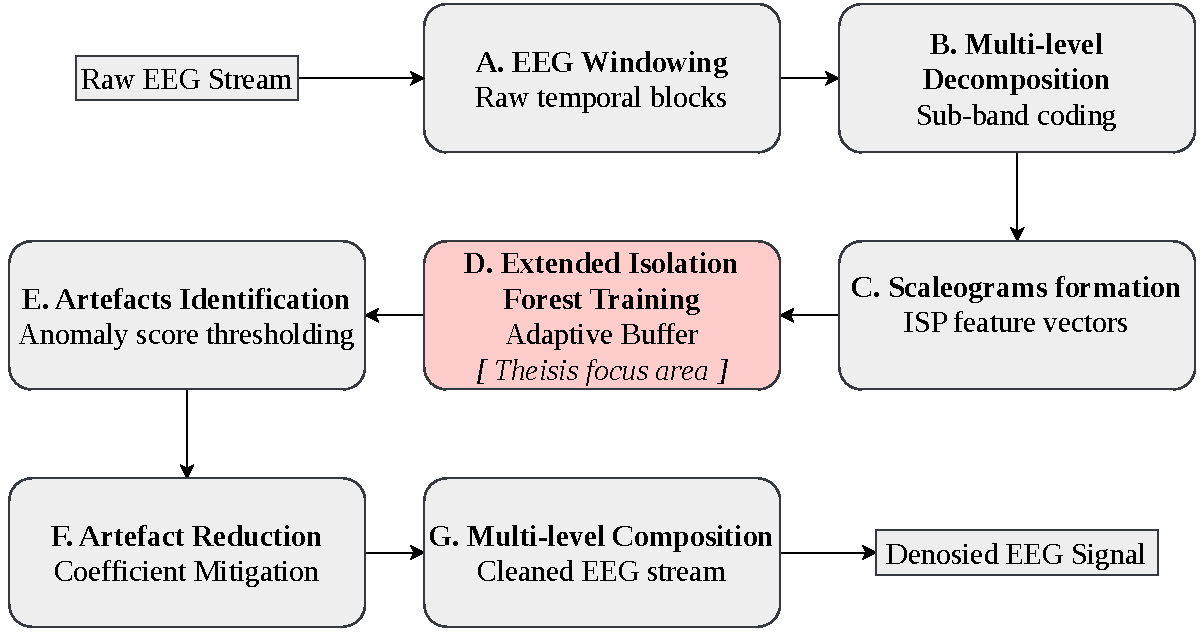
\includegraphics[width=\textwidth]{Figures/oneegwavelad_pipeline_focus.pdf}
    \vspace{0.5em}\hrule
    \caption{The seven-phase architecture of the onEEGwaveLAD pipeline~\parencite{longo2025oneegwavelad}. Phase D is highlighted in red to mark the exclusive focus of this thesis: optimizing the Adaptive Buffer Size ($B_s$) that governs how much historical context feeds the anomaly detection engine. All other phases and parameters are held constant throughout the grid search.}
    \label{fig:oneegwavelad_pipeline_focus}
    \vspace{0.5em}\hrule
\end{figure}

\begin{table}[!htb]
    \centering
    \small
    \begin{tabularx}{\textwidth}{@{} >{\raggedright\arraybackslash}p{3.8cm} >{\raggedright\arraybackslash}p{2.4cm} >{\raggedright\arraybackslash}X @{}}
        \toprule
        \textbf{Parameter / Variable} & \textbf{Value} & \textbf{Role and Classification} \\
        \midrule
        \multicolumn{3}{l}{\textit{\textbf{Independent Variable}}} \\
        Adaptive Buffer Size ($B_s$) & Stage 1: $\{1,2,4,$ $8,16,32,64\}$ Stage 2: $\{4,6,8,$ $10,12,14,$ $16,18\}$ & \textbf{Independent variable.} Two-stage grid search: Stage 1 (logarithmic, 7 points); Stage 2 (linear refinement around elbow, 8 points: $B_s \in \{4,6,8,10,12,14,16,18\}$). \\
        \addlinespace
        \multicolumn{3}{l}{\textit{\textbf{Comparison Methods \& Dependent Variables}}} \\
        12 methods total & 7 + 5 & 7 buffer configs + 5 baselines (FASTER, 4 ASR variants). \\
        Denoising performance & 15 metrics (10 + 5) & Time-domain (SNR-Diff, PSNR-Diff, RMSE), statistical (CC, MI), frequency-domain (BPPE, MSC). Behavioural classification: 10 similarity-preservation metrics (monotonic convergence); 5 artefact-removal metrics (non-monotonic at large $B_s$). \\
        \addlinespace
        \multicolumn{3}{l}{\textit{\textbf{Controlled Variables (onEEGwaveLAD Parameters)}}} \\
        $RTW_L$ / $S_r$ & 1000ms / 1024Hz & Real-time window length; native sampling rate. \\
        $MW$ & \texttt{sym4} & Symlets-4 wavelet; \texttt{periodization} mode. \\
        $IF_s$ / $IF_t$ & 512 / 100 & eiFOREST sub-sampling size; number of trees. \\
        $T_a$ / $E_s$ & 0.55 / 35 & Anomaly threshold; expansion step. \\
        Random seed & 42 & Reproducibility; forest retrains every 5 windows. \\
        \bottomrule
    \end{tabularx}
    \caption{Experimental design and parameter instantiation. The Adaptive Buffer Size ($B_s$) is swept across a two-stage grid: Stage 1 identifies the approximate elbow region via logarithmic sampling; Stage 2 refines around that region with linear spacing. Denoising performance (15 metrics) serves as the dependent variable, with 10 metrics exhibiting similarity-preservation behaviour and 5 exhibiting artefact-removal behaviour (detailed in Section~\ref{sec:evaluation_workflow}). All other parameters remain constant.}
    \label{tab:instantiation}
\end{table}

\subsection{Parameterisation of DWT and Scaleogram Construction}
\label{subsec:param_dwt_scaleogram}
 
Each streamed block is decomposed with a multi-level Discrete Wavelet Transform implemented through the PyWavelets library~\parencite{lee2019pywavelets}. The Symlets-4 (\texttt{sym4}) wavelet was selected as the analysing filter, a near-symmetric member of the Daubechies family~\parencite{daubechies1992ten} whose reduced phase distortion is well suited to preserving the temporal position of transient events in the reconstructed signal. Boundary handling uses the \texttt{periodization} mode, which keeps the number of coefficients strictly consistent with the dyadic block length established in Section~\ref{sec:data_prep_streaming} and so avoids the coefficient growth introduced by zero-padded extensions. The number of decomposition levels is not fixed manually but obtained from \texttt{pywt.dwt\_max\_level} for the given block length, so the decomposition proceeds to the deepest level the signal supports without the analyst imposing an arbitrary depth.

The coefficients returned by the transform are then arranged into the normalised scaleogram that the anomaly detector consumes. Because coefficients at deeper levels carry systematically larger magnitudes than those at shallow levels, each coefficient is divided by $2^{m}$, with $m$ the decomposition level, to place the levels on a comparable scale before any distance is computed. To reconcile the differing number of coefficients across levels, the values at each level are up-sampled with \texttt{np.repeat} so that every level contributes the same number of columns, yielding a rectangular matrix whose vertical slices are the Instantaneous Spectral Profiles used throughout the remainder of the pipeline. The normalised scaleogram consumed by the anomaly detector is assembled exclusively from the detail coefficients of the decomposition. The approximation coefficients of the deepest level, which carry the slowest components of the signal, are held aside and passed through to reconstruction unchanged; they take no part in the anomaly scoring or in the subsequent attenuation. As with the normalisation, this separation ensures that the representation used for detection does not alter the coefficients later used to rebuild the denoised signal, and the consequence of leaving the approximation band unprocessed is examined among the limitations in Section~\ref{sec:assumptions_strengths_limitations}.

\subsection{Engineering the Adaptive Sliding Buffer Mechanism}
\label{subsec:eng_sliding_buffer}
 
The temporal adaptivity of the framework is realised by a first-in, first-out buffer that stores the Instantaneous Spectral Profiles of the most recent windows, its depth fixed by the Adaptive Buffer Size ($B_s$)~\parencite{longo2025oneegwavelad}. As each new window arrives, its profiles are appended and the oldest are discarded, so the isolation model is always trained on a sliding, contiguous stretch of recent history rather than on the full recording. This design gives the detector a moving reference of nominal activity that tracks slow changes in the signal, while bounding the amount of data held in memory at any instant, a property required for continuous operation on modest hardware.

Retraining the isolation model on every single window would, however, dominate the per-window computation and place the per-window latency beyond the range acceptable for real-time use. To contain this cost, the model is refitted once every five windows rather than continuously, the buffer being updated at each step but the isolation trees rebuilt only when the window counter satisfies \texttt{window\_cnt \% 5 == 0}. This throttling trades a small amount of responsiveness to the most recent samples for a substantial reduction in processing time, and its consequences for the framework's sensitivity to abrupt changes are examined among the limitations in Section~\ref{sec:assumptions_strengths_limitations}.

\subsection{Integration and Reconstruction with the eiFOREST}
\label{subsec:integration_eiforest}
 
Anomaly detection is delegated to the Extended Isolation Forest as implemented in the \texttt{isotree} library~\parencite{cortes2019distance}. The ensemble is fixed at $IF_t = 100$ trees with a sub-sampling size of $IF_s = 512$ profiles, and the random seed is set to $42$ so that every run over the grid is reproducible. Each Instantaneous Spectral Profile of the current window is assigned an anomaly score, and profiles whose score exceeds the anomaly threshold $T_a = 0.55$ are recorded as anomalous time locations; the value $0.55$ is applied uniformly across all subjects and channels and is therefore treated as a fixed control rather than a tuned
quantity.

Mitigation operates on the original, unnormalised detail coefficients so the reconstructed signal is not distorted by the normalisation used for detection. Let $\mu$ denote the centroid of the coefficient vectors held in the buffer, and let $c_i$ be the coefficient vector at an anomalous time location together with the neighbours added by the expansion step $E_s = 35$. An attenuation factor is formed from the distance of each vector to the centroid, normalised by the largest such distance~\parencite{longo2025oneegwavelad}:
\begin{equation}
    m_i = 1 - \frac{\lVert c_i - \mu \rVert}{\max_j \lVert c_j - \mu \rVert},
    \label{eq:mitigator}
\end{equation}
and the mitigated coefficients are obtained by an element-wise (Hadamard) product~\parencite{longo2025oneegwavelad}:
\begin{equation}
    \tilde{c}_i = m_i \odot c_i, \qquad m_i \in [0,1],
    \label{eq:mitigation_apply}
\end{equation}
where the factors are clipped to the interval $[0,1]$ (\texttt{np.clip(mtga\_vec, 0.0, 1.0)}) so mitigation can only reduce, never amplify, a coefficient.\footnote{The originating framework defines the central reference of the buffer as its medoid~\parencite{longo2025oneegwavelad}; the present implementation uses the centroid, a lower-complexity approximation that the framework's authors permit and that avoids the pairwise dissimilarity computation required by the medoid.} Coefficients closer to the centroid are attenuated less and those further away more, so profiles judged anomalous are drawn toward the representative activity of the recent buffer. The retained and attenuated detail coefficients, together with the unchanged approximation coefficients, are then returned to the time domain by the inverse Discrete Wavelet Transform, producing the denoised window that the streaming loop emits before the next block is drawn.


\subsection{Design of the Adaptive Buffer Size Grid Search}
\label{subsec:design_grid_search}

With every other component held constant, the Adaptive Buffer Size is the single independent variable of the experiment and is varied over a two-stage grid search strategy designed to balance computational efficiency with resolution in the region where the convergence lower bound is expected to lie.

\textbf{Coarse-grained exploration.} The initial search spans $B_s \in \{1, 2, 4, 8, 16, 32, 64\}$, covering two orders of magnitude with exponential spacing on a logarithmic scale (base-2). This geometric progression allocates dense sampling to the shallow buffers where performance is anticipated to change rapidly, and progressively coarser steps across the deeper buffers where performance is expected to converge. The coarse grid provides a preliminary view of the convergence trajectory and locates the approximate region of diminishing returns without evaluating every intermediate integer, which would be computationally prohibitive across thirty subjects and thirty channels.

\textbf{Fine-grained refinement.} Following the identification of the coarse elbow region around $B_s \approx 4$ in the logarithmic Phase 1 search, a second linear grid was executed to provide higher resolution within the converging interval. This refined Phase 2 grid spans $B_s \in \{4, 6, 8, 10, 12, 14, 16, 18\}$, with uniform spacing of two units, and captures the transition from rapid improvement to plateau with sufficient granularity to support precise Kneedle detection and to confirm that the convergence lower bound lies at $B_s = 8$ rather than at the Phase 1 approximate elbow of $B_s = 4$. The shift from logarithmic to linear spacing in the refined grid acknowledges the sensitivity of the Kneedle elbow detection to the axis scale~\parencite{satopaa2011finding}, a methodological consideration addressed in the discussion of results. The two grids share three overlapping points ($B_s \in \{4,8,16\}$), which serve as consistency checks: if the convergence lower bound is robust, it should be identifiable from both the coarse and refined perspectives despite the difference in axis scale and sampling density. Both stages are executed on the full cohort of thirty subjects, so that the reported convergence lower bound reflects the behaviour across the entire dataset rather than a subset.

\begin{table}[!htb]
    \centering
    \renewcommand{\arraystretch}{1.3}
    \begin{tabular}{@{} l p{5.2cm} p{5.2cm} @{}}
        \toprule
        \textbf{Feature} & \textbf{Coarse-grained Stage} & \textbf{Fine-grained Stage} \\
        \midrule
        \textbf{Grid} & $\{1,2,4,8,16,32,64\}$ & $\{4,6,8,10,12,14,16,18\}$ \\
        \textbf{Spacing} & Exponential & Linear \\
        \textbf{Axis scale} & Logarithmic (base-2) & Linear \\
        \textbf{Purpose} & Identify approximate convergence region & Precisely locate lower bound within region \\
        \bottomrule
    \end{tabular}
    \caption{Two-stage grid search strategy for locating the convergence lower bound. The 
coarse stage covers two orders of magnitude efficiently, while the refined stage provides 
higher resolution in the region identified by the coarse search ($B_s \approx 8$). The two stages share three overlapping points ($B_s \in \{4,8,16\}$), which serve as consistency checks: if the convergence lower bound is robust, it should be identifiable from both the coarse and refined perspectives despite the difference in axis scale and sampling density.}
    \label{tab:two_stage_grid}
\end{table}
Because the seven buffer sizes of the coarse grid, combined with the eight of the refined grid (with overlap at 4, 8, 16), thirty channels and thirty subjects define a large number of independent denoising runs, the search is executed in parallel. Each combination of subject, channel and buffer size is flattened into a self-contained task and dispatched across all available cores with the \texttt{joblib} library, with the forest itself also permitted to use all cores. Partial results are appended to disk as each task completes, so an interrupted run can resume from the last checkpoint rather than restart, a practical safeguard given the length of the full grid. The per-window execution time is recorded alongside the denoising metrics for every task, providing the latency measurements later used to judge real-time viability.

\section{Deployment and Implementation Environment}
\label{sec:deployment_environment}
 
The experiments were executed on the Google Colaboratory platform, with the dataset and all intermediate artefacts stored on a mounted Google Drive volume under a fixed project directory. This arrangement was chosen for its reproducibility and for the persistent storage it provides across sessions. Because the full sweep over seven buffer sizes, thirty channels and thirty subjects spans a large number of independent runs, partial results are appended to disk as each task completes, allowing an interrupted execution to resume from the last written checkpoint rather than restart. The denoising metrics for every task, along with the per-window latency used later to judge real-time viability, are accumulated in comma-separated result files that are consolidated into the master table on which the statistical analysis operates.

The processing pipeline is implemented in Python and rests on a small set of established scientific libraries, each confined to a well-defined role. Neurophysiological input and event extraction are handled by MNE-Python~\parencite{gramfort2013meg}; the multi-level wavelet decomposition and its inverse are computed with PyWavelets~\parencite{lee2019pywavelets}; the Extended Isolation Forest is provided by the \texttt{isotree} library~\parencite{cortes2019distance}; and the non-parametric statistical procedures draw on \texttt{scipy} and \texttt{scikit\_posthocs}~\parencite{virtanen2020scipy, terpilowski2019scikit}. The baseline methods draw on the \texttt{asrpy} implementation of Artefact Subspace Reconstruction and the FASTER-style routines supplied with the study material~\parencite{mullen2015real, nolan2010faster}. Channel-level parallelism is realised with \texttt{joblib}, which dispatches the flattened subject--channel--buffer tasks across all available cores, with the isolation forest itself also permitted to use every core during fitting. The complete software stack and the responsibility assigned to each component are listed in Table~\ref{tab:software_stack}.

\section{Baseline Denoising Methods}
\label{sec:baseline_methods}
 
Assessing the effect of the buffer size in isolation establishes how onEEGwaveLAD behaves internally, but it does not indicate how that behaviour compares with denoising methods already established in the literature. To provide this external reference, and following the evaluation design of the framework's originating study~\parencite{longo2025oneegwavelad}, five automated baselines are evaluated alongside the seven buffer configurations under an identical preprocessing and scoring procedure. All five operate without manual intervention, matching the automated, reference-free character that the online setting demands, and each produces a denoised thirty-channel output that is average-re-referenced in the same manner as the onEEGwaveLAD outputs before evaluation. The methods and their principal settings are summarised in Table~\ref{tab:baselines}.

\begin{table}[!htb]
    \centering
    \begin{tabularx}{\textwidth}{@{} l l l X @{}}
        \toprule
        \textbf{Method} & \textbf{Family} & \textbf{Regime} & \textbf{Principal settings} \\
        \midrule
        FASTER & Automatic ICA & -- & Five-property rejection (spatial kurtosis, band slope, Hurst exponent, maximum gradient, VEOG correlation); rejection threshold $z = 3$. \\
        \addlinespace
        ASR\_offline\_13 & Subspace reconstruction & Offline & Calibration on full recording with pre-cleaning; cutoff $13$. \\
        ASR\_offline\_20 & Subspace reconstruction & Offline & Calibration on full recording with pre-cleaning; cutoff $20$. \\
        ASR\_online\_13 & Subspace reconstruction & Online & Calibration on twenty one-second windows; cutoff $13$. \\
        ASR\_online\_20 & Subspace reconstruction & Online & Calibration on twenty one-second windows; cutoff $20$. \\
        \bottomrule
    \end{tabularx}
    \caption{The five automated baseline denoising methods evaluated alongside the seven
    onEEGwaveLAD buffer configurations. All methods share the preprocessing and scoring procedure
    described in Sections~\ref{sec:data_prep_streaming} and~\ref{sec:evaluation_workflow}, and are
    ranked jointly with onEEGwaveLAD in the non-parametric analysis. FASTER configuration follows~\textcite{nolan2010faster}; ASR parameter selection and calibration regimes follow~\textcite{mullen2015real}.}
    \label{tab:baselines}
\end{table}

The first baseline is an automatic Independent Component Analysis procedure in the style of the FASTER pipeline~\parencite{nolan2010faster}. It decomposes the signal, characterises each component through a set of statistical properties, and rejects those flagged as artifactual before reconstructing the signal from the remainder. The rejection combines five descriptors, comprising a spatial kurtosis, a slope in the filter band, the Hurst exponent, a measure of maximum gradient and a correlation with the vertical electrooculographic channel, and a component is discarded when its standardised value on these descriptors exceeds a threshold of three. The vertical EOG derivation therefore serves here as the means of identifying ocular components, which is the role for which it is retained in the dataset.

The remaining four baselines are variants of Artefact Subspace Reconstruction, a method that identifies high-variance segments relative to a calibrated model of clean data and reconstructs them from the retained subspace~\parencite{mullen2015real}. Two dimensions are varied. The first is the calibration regime: an offline variant calibrates on the full recording and pre-cleans it, whereas an online variant calibrates on a limited number of one-second windows to mimic a system that must begin operating without access to the entire session. The second is the cutoff parameter that sets how aggressively segments are reconstructed, evaluated at values of thirteen and twenty. Crossing these two dimensions yields the four configurations reported here, namely the offline and online regimes each at cutoffs of thirteen and twenty. Together with the FASTER-style procedure, these baselines span both retrospective and streaming operation, providing a reference against which the buffer-size behaviour of onEEGwaveLAD is judged within the common statistical analysis described in Section~\ref{sec:evaluation_workflow}.

\section{Evaluation Workflow}
\label{sec:evaluation_workflow}

The evaluation workflow converts each denoised window into quantitative scores and submits those scores to a three-tier statistical strategy, where each tier addresses a distinct research question. The design is shaped by two requirements. First, the ERP-CORE recordings provide no perfectly clean reference against which a denoised signal can be compared directly, so the notions of signal and noise required by the error metrics must be operationalised from the event structure of the data. Second, the metrics span heterogeneous scales and directions of merit, so they must be converted into a common ranking before any method can be declared superior. The three tiers of analysis, summarised in Table~\ref{tab:three_tier_analysis}, play complementary roles in establishing the convergence lower bound and situating it relative to established denoising methods.

\begin{table}[!htb]
    \centering
    \begin{tabularx}{\textwidth}{@{} >{\raggedright\arraybackslash}p{3.0cm} >{\raggedright\arraybackslash}p{4.0cm} >{\raggedright\arraybackslash}X @{}}
        \toprule
        \textbf{Analysis tier} & \textbf{Research question} & \textbf{Role in synthesis} \\
        \midrule
        \textbf{Baseline comparison} (12 methods: 7 buffer configurations + 5 baselines) & 
        Is onEEGwaveLAD effective? From which buffer size does it match or exceed FASTER and ASR? & 
        \textbf{Core:} Establishes the practical significance of the convergence lower bound by 
        demonstrating that it corresponds to the threshold at which onEEGwaveLAD attains 
        competitive performance. \\
        \addlinespace
        \textbf{Convergence bound identification} (applied to raw metric trajectories) & 
        At which buffer size do the metric values cease to change meaningfully? & 
        \textbf{Core:} Locates the convergence lower bound through the multi-criteria protocol 
        (absolute criterion, noise floor, Kneedle elbow). \\
        \addlinespace
        \textbf{Directional significance} (7 buffer configurations only) & 
        Does buffer size have a statistically significant effect, and in which direction? & 
        \textbf{Supporting:} Confirms that buffer size is a relevant hyperparameter and that 
        larger buffers yield better aggregate performance, validating the premise of the search. \\
        \bottomrule
    \end{tabularx}
    \caption{The three-tier analysis strategy employed to test the research hypothesis of 
    Section~\ref{subsec:literature_gaps_hypotheses} and locate the convergence lower bound. 
    Each tier addresses a distinct question; the baseline comparison and convergence bound 
    identification are the core analyses, while the directional test provides supporting 
    evidence that buffer size matters.}
    \label{tab:three_tier_analysis}
\end{table}

The following subsections describe how the metric suite is computed in code under these constraints, how the raw metric values are converted into ranks that can be aggregated across 
heterogeneous scales, and how the resulting ranks are tested for statistical significance.

\subsection{Automated Batch Evaluation Metrics Formulation}
\label{subsec:automated_batch_metrics}
 
The evaluation is performed by a dedicated batch module that receives, for every combination of subject, channel and buffer size, the original and denoised signals together with the stimulus events extracted during ingestion. The seven metric families, namely the difference in SNR and PSNR, RMSE, Pearson correlation, mutual information, band power preservation error and magnitude squared coherence, are each computed for the window under assessment. Because band power preservation error and coherence are evaluated separately for the delta, theta, alpha, beta and gamma bands, the seven families expand into fifteen scalar quantities per denoised signal, providing complementary views of amplitude fidelity, statistical dependence and spectral preservation. All fifteen are written to a master results table alongside the recorded per-window latency, so the statistical analysis operates on a single, uniform record for the entire grid.

The fifteen scalar quantities can be organised into two principal categories that differ in their directional preferences and in the aspect of denoising quality they assess. The similarity-oriented category, comprising ten metrics (Pearson correlation, mutual information, RMSE, the five band power preservation errors, and magnitude squared coherence in the alpha and beta bands), measures how closely the denoised signal preserves the structure of the original recording; these metrics generally favour larger buffers that provide a stable reference for the anomaly detector and exhibit monotonically improving trajectories as $B_s$ increases. The artefact-removal category, comprising five metrics (the differences in SNR and PSNR computed from the event-locked responses, and magnitude squared coherence in the gamma, theta and delta bands), assesses the enhancement of the signal-to-noise ratio attributable to denoising; these metrics favour smaller buffers that aggressively attenuate contamination and exhibit non-monotonic behaviour at large $B_s$, where the conservative mitigation applied to stable buffers removes less artefactual energy. This heterogeneity affects the aggregation strategy, as discussed in  Section~\ref{subsec:convergence_lower_bound}, and is revisited among the limitations in Section~\ref{sec:assumptions_strengths_limitations}. To aid interpretation of the convergence analysis reported in Chapter~\ref{chap:results}, Figure~\ref{fig:metric_categories} organises the fifteen metrics by their directional preferences and behavioural characteristics across the buffer size grid.

\begin{figure}[!htb]
\hrule\vspace{0.5em}
    \centering
    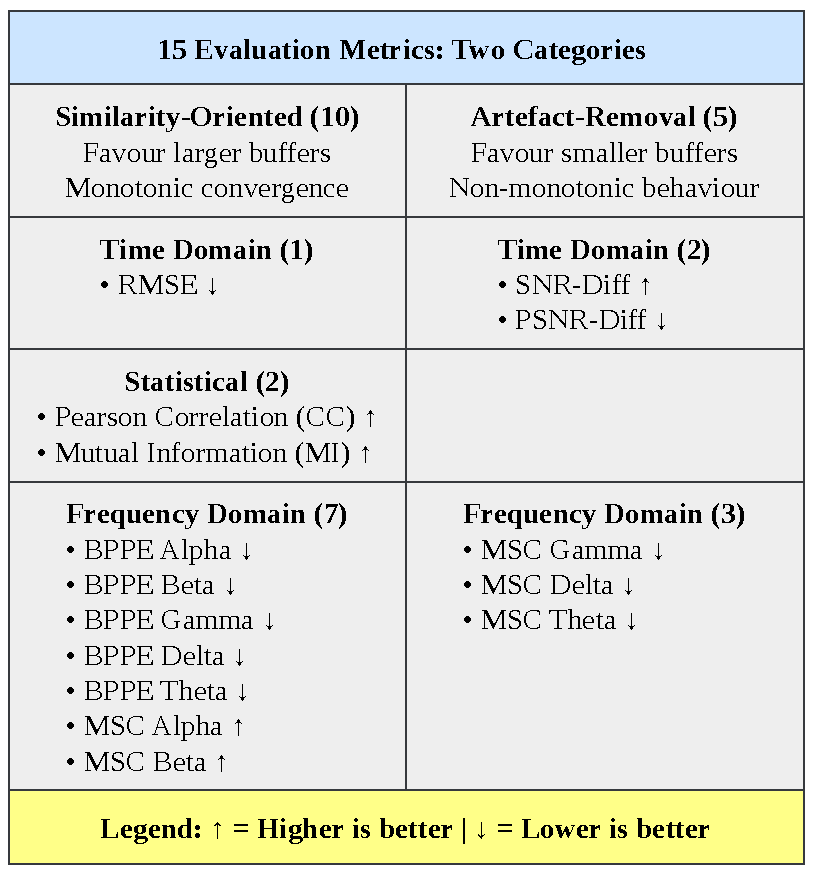
\includegraphics[width=0.85\textwidth]{Figures/metric_categories.pdf}
    \vspace{0.5em}\hrule
    \caption{Organisation of the fifteen evaluation metrics into similarity-oriented and artefact-removal categories. The similarity-oriented majority (ten metrics) favour larger buffers and exhibit monotonic improvement trajectories, whereas the artefact-removal minority (five metrics) favour smaller buffers and exhibit non-monotonic behaviour at large $B_s$. This heterogeneity motivates the category-stratified convergence analysis and the use of median aggregation as a robustness check, as detailed in Section~\ref{subsec:convergence_lower_bound}.}
    \label{fig:metric_categories}
    \vspace{0.5em}\hrule
\end{figure}

This categorisation is not merely a post-hoc observation but reflects a fundamental tension in denoising evaluation: metrics that assess signal preservation reward conservative processing (larger buffers), whereas metrics that assess artefact suppression reward aggressive attenuation (smaller buffers). The divergent behaviour of these two families, and its implications for identifying the convergence lower bound, is addressed in detail in Section~\ref{subsec:convergence_lower_bound} and Section~\ref{subsec:experimental_limitations}.


\subsubsection{Computation of Time-Domain Errors (SNR, PSNR, RMSE)}
\label{subsubsec:computation_time_domain}
 
The central difficulty in computing the signal-to-noise metrics of Equations~\ref{eq:snr}--\ref{eq:psnr} is the absence of a ground-truth clean signal in a naturalistic recording. Rather than estimating the removed energy as noise, which would reward indiscriminate smoothing, the module uses the event structure of the recording as the reference. Using the stimulus markers obtained through \texttt{mne.events\_from\_annotations}, the signal term is taken from the stimulus-locked response and the noise term from the pre-stimulus baseline variance, so the resulting figures reflect the preservation of a physiological response relative to its own baseline. The differences $\mathrm{SNR}_{\mathrm{diff}}$ and $\mathrm{PSNR}_{\mathrm{diff}}$ between the raw and denoised signals are reported, as defined in Section~\ref{subsec:time_domain_metrics}, while RMSE (Equation~\ref{eq:rmse}) is computed directly between the two time series. In this real-mode evaluation the reference and the raw signal are both taken from the average-re-referenced original recording, and the denoised signal is the average-re-referenced output of the method under assessment, so that all three are expressed on a common footing. A consequence of this event-based definition is that the signal-to-noise figures are only defined for recordings that carry usable stimulus annotations, a delimitation returned to in Section~\ref{sec:assumptions_strengths_limitations}.

\subsubsection{Computation of Statistical Similarity (Pearson Corr. and MI)}
\label{subsubsec:computation_statistical}
 
The statistical metrics quantify how much of the structure of the original signal survives denoising, independently of absolute amplitude. The Pearson correlation coefficient (Equation~\ref{eq:cc}) is computed between the original and denoised time series to measure linear waveform agreement, while mutual information (Equation~\ref{eq:mi}) captures non-linear dependence that correlation alone cannot express. Both are obtained per window from the paired samples of the two signals, so a loss of shared structure, whether through over-attenuation or through the injection of spurious activity, is registered as a reduction in the corresponding score. Because a higher value denotes greater preservation for both, these two quantities enter the ranking with the same orientation and require no sign adjustment.

\subsubsection{Computation of Spectral Preservation (BPPE and MSC)}
\label{subsubsec:computation_spectral}
 
The spectral metrics assess whether denoising distorts the distribution of energy across the clinical frequency bands. Band power preservation error (Equation~\ref{eq:bppe}) is computed as the relative deviation in band power between the original and denoised signals for each of the delta, theta, alpha, beta and gamma bands, and magnitude squared coherence (Equation~\ref{eq:msc}) is evaluated over the same bands. As noted in Section~\ref{subsec:frequency_domain_metrics}, coherence estimated over a single continuous block degenerates to unity, so it is computed with Welch's method of overlapping, averaged segments. The segment length is set from a baseline of $2048$ samples and clipped to the available signal length at run time, taking $n_{\mathrm{perseg}} = \min(2048, N)$ with $N$ the number of paired samples; within a short online window this averaging necessarily lowers the frequency resolution, a trade-off accepted so coherence remains well defined. These band-resolved quantities are interpreted according to the role of each band. Coherence in the alpha and beta bands is treated as a signal to be preserved, so a higher value is better, whereas coherence in the delta, theta and gamma bands is treated as reflecting ocular and muscular contamination, so a lower value, indicating that this interference no longer tracks the reference, is better. The band power preservation errors are minimised in every band. This orientation is made explicit because it determines the direction in which each metric enters the ranking.

\subsection{Non-Parametric Statistical Tests Strategy}
\label{subsec:non_parametric_tests}

The denoising scores cannot be assumed to be normally distributed across subjects and channels, so the comparison of methods relies on non-parametric procedures applied to ranks rather than to raw values. The aggregation follows a rank-then-aggregate protocol~\parencite{friedman1937use}: at the lowest level, each of the fifteen metrics is converted into a rank for every channel of every subject, with a rank of one consistently denoting the best-performing configuration regardless of the native orientation of the metric (metrics for which a lower value denotes better performance, such as RMSE, the PSNR difference and the band power preservation errors, are sign-inverted before ranking, so that the rank order is uniform). Critically, this ranking operation is performed \emph{before} any aggregation: within each subject--channel--metric combination, the twelve methods are ranked from 1 (best) to 12 (worst) on the raw metric values, and only then are these \emph{rank} values averaged--first across the fifteen metrics to yield a composite rank per channel, and subsequently across channels and subjects according to one of three complementary configurations that differ in whether subjects and channels are treated individually or pooled. This rank-then-aggregate order ensures that metrics with heterogeneous scales and opposing directional preferences are reconciled into a common ordinal comparison before any averaging occurs, preventing any single metric from dominating the composite score by virtue of its numerical range.

The ranked scores are organised under three aggregations, each of which ranks the twelve methods (namely the seven buffer configurations and the five baselines) jointly. In the first, metric-aggregated and single-subject, each subject is analysed in isolation: the ranks of the fifteen metrics are averaged within each channel, yielding a $30 \times 12$ matrix of channels against methods that is tested separately for every subject. In the second, channel-specific and multiple-subjects, the subjects are pooled while the channel dimension is retained, so that each channel of each of the thirty subjects contributes an independent row and the rank matrix has shape $900 \times 12$. In the third, channel-aggregated and multiple-subjects, the channel ranks are further averaged within each subject to form a single composite row per subject, giving a $30 \times 12$ matrix that assesses the methods at the subject level. These configurations, and the tests applied to each, are summarised in Table~\ref{tab:statistical_tests}.

\begin{table}[!htb]
    \centering
    \begin{tabularx}{\textwidth}{@{} 
        >{\raggedright\arraybackslash}p{3.5cm} 
        l 
        >{\raggedright\arraybackslash}p{2.0cm} 
        >{\raggedright\arraybackslash}X 
        l 
        @{}}
        \toprule
        \textbf{Configuration} & \textbf{Test} & \textbf{Post-hoc} & \textbf{Aggregation} & \textbf{Shape} \\
        \midrule
        Metric-aggregated / single-subject & Friedman & Wilcoxon + Holm, and Nemenyi & Subjects analysed individually; metric ranks averaged within each channel. & $30 \times 12$ \\
        \addlinespace
        Channel-specific / multiple-subjects & Friedman & Nemenyi & Subjects pooled; metric ranks averaged within each channel, channel dimension retained. & $900 \times 12$ \\
        \addlinespace
        Channel-aggregated / multiple-subjects & Friedman & Nemenyi & Subjects pooled; channel ranks further averaged into one composite row per subject. & $30 \times 12$ \\
        \bottomrule
    \end{tabularx}
    \caption{Non-parametric statistical configurations used to compare the twelve methods, namely
the seven buffer configurations and the five baselines. The rank-then-aggregate protocol is 
applied uniformly: at the lowest level, each of the fifteen metrics is ranked per channel 
(rank~1~=~best), and these ranks are then aggregated by averaging according to the configuration. 
Each configuration applies the Friedman test and differs in whether subjects and channels are 
analysed individually or pooled; the matrix shape follows from the thirty subjects and thirty 
channels.}
    \label{tab:statistical_tests}
\end{table}

Global significance is assessed in every configuration with the Friedman test, a non-parametric analogue of the repeated-measures analysis of variance suitable for ranked data~\parencite{friedman1937use}, applied through \texttt{scipy.stats.friedmanchisquare}. The test evaluates whether the twelve methods share the same average rank against the alternative that at least one differs, with the statistic approximately chi-squared distributed under the null across the methods. Assessing it under the three aggregations described above distinguishes effects that hold at the level of individual subjects, that persist across the electrode space when subjects are pooled, and that survive once channels are summarised into a
single per-subject value.

A significant Friedman result establishes that the methods differ but does not identify which pairs are responsible. Across all three configurations the Nemenyi post-hoc test is applied through \texttt{scikit\_posthocs.posthoc\_nemenyi\_friedman}, which declares two methods significantly different when the gap between their average ranks exceeds the critical difference at the chosen significance level, and whose outcome is rendered as a critical difference diagram in the results chapter. For the single-subject configuration, where a within-subject post-hoc test must contend with far fewer observations, the Nemenyi comparison is complemented by the Wilcoxon signed-rank test~\parencite{wilcoxon1945individual} applied to each pair of methods, with the resulting $p$-values corrected for multiple comparisons through the Holm--Bonferroni procedure~\parencite{holm1979simple} (\texttt{method='holm'}) to control the family-wise error rate. This layered strategy provides a global test in each configuration, two independent accounts of the per-subject pairwise differences, and an aggregated view across the full cohort.

The rank-based tests described above establish that the buffer configurations differ significantly and delimit the region within which performance is statistically distinguishable, but they do not themselves locate the convergence lower bound. Because ranks compress the distances between configurations, a rank-based view alone can obscure the point at which the underlying metric values level off. The convergence lower bound is therefore identified through the multi-criteria protocol applied to the raw metric trajectories, as detailed in Section~\ref{subsec:convergence_lower_bound}, with the Friedman and Nemenyi procedures serving as supporting evidence that confirms the statistical significance of the differences observed in those trajectories. Reporting both the rank-based significance and the convergence of the raw values provides complementary perspectives from which the lower bound is triangulated in the results chapter: the former demonstrates that the methods differ at all, while the latter locates where that difference ceases to be material.

\subsection{Convergence Lower Bound Identification Protocol}
\label{subsec:convergence_lower_bound}

While the Friedman and Nemenyi procedures described above test whether the buffer configurations differ at all and which of them are separated by a statistically significant margin, they operate on rank statistics that compress the distances between configurations and can obscure the point at which the underlying metric values converge. The convergence lower bound is therefore located on the trajectories of the raw metric values themselves, rather than on the rank statistics, using a multi-criteria protocol that combines three complementary approaches to assess when further increases in buffer size yield no material further gain. Initial attempts to locate convergence using a simple threshold-based criterion (normalised improvement falling below a fixed threshold $\tau$) proved unsuccessful, as the gradual levelling and heterogeneity across metrics prevented a clean determination of the convergence point; the composite protocol described below was developed to address this limitation by triangulating the threshold through statistical, geometric, and category-stratified analyses.

\subsubsection{Absolute Criterion and Noise Floor}

For each metric $m$, let $v_m(B_s)$ denote the mean value across channels and subjects at buffer 
size $B_s$, with polarity adjusted according to Table~\ref{tab:instantiation} so that larger 
values consistently denote better performance. The normalised improvement between successive 
buffer sizes is computed as
\begin{equation}
    \Delta_m(B_{s,i} \to B_{s,i+1}) = \frac{v_m(B_{s,i+1}) - v_m(B_{s,i})}{\max_{B_s} v_m(B_s) - \min_{B_s} v_m(B_s)},
    \label{eq:normalised_improvement}
\end{equation}
which scales the raw change by the full range of the metric so that improvements across 
heterogeneous metrics can be compared on a common footing. The absolute criterion 
declares that convergence has occurred when the mean improvement falls below the threshold set 
by random variation,
\begin{equation}
    |\text{mean}\,\Delta| < 1.96 \cdot \text{SE}(\Delta),
    \label{eq:absolute_criterion}
\end{equation}
where the factor $1.96$ corresponds to the critical value of the standard normal distribution at 
the $95\%$ confidence level, and $\text{SE}(\Delta)$ is the standard error of the improvement 
computed across the metrics. A complementary noise floor is defined as the expected 
absolute deviation under the null hypothesis that the changes are drawn from a zero-mean 
distribution,
\begin{equation}
    \mathbb{E}[|\Delta|] = \text{SE}(\Delta) \cdot \sqrt{\frac{2}{\pi}},
    \label{eq:noise_floor}
\end{equation}
which follows from the properties of the half-normal distribution. Improvements that fall below 
this floor are attributed to measurement noise rather than to systematic changes induced by the 
buffer size.

\subsubsection{Kneedle Elbow Detection}

The absolute criterion and noise floor assess convergence in terms of statistical thresholds, but they do not explicitly identify the point of diminishing returns where the trajectory transitions from rapid improvement to gradual levelling. To locate this transition, the parameter-free Kneedle algorithm~\parencite{satopaa2011finding}, which locates the elbow through geometric curvature without requiring manual specification of a sensitivity threshold, is applied to the gain curve, defined as the improvement in each metric relative to the baseline configuration $B_s = 1$, expressed in units of the cross-subject standard deviation. The Kneedle method fits a smooth curve to the gain trajectory and identifies the point of maximum curvature, which corresponds to the elbow where marginal returns begin to diminish sharply. Because the algorithm is sensitive to the axis scale, the coarse-grained search employs a logarithmic (base-2) horizontal axis to reflect the exponential spacing of the buffer grid, while the fine-grained refinement uses a linear axis to match the equally spaced grid in the convergence region. The elbow points identified by the two  stages are reported separately and their consistency assessed as a robustness check.

\subsubsection{Metric Category Stratification and Aggregation Pipelines}

The fifteen metrics are not homogeneous in their directional preferences. As detailed in Section~\ref{subsec:automated_batch_metrics}, the ten similarity-oriented metrics (Pearson correlation, mutual information, RMSE, five band power preservation errors, and magnitude squared coherence in the alpha and beta bands only) exhibit a preference for larger buffers and monotonic improvement that asymptotically approaches a noise floor, whereas the five artefact-removal metrics (SNR-Diff, PSNR-Diff, and magnitude squared coherence in the theta, gamma, and delta bands) favour smaller buffers and exhibit non-monotonic behaviour at large $B_s$. The inclusion of MSC theta, gamma, and delta in the artefact-removal category reflects their observed directional preference for smaller buffers, aligning with SNR-Diff and PSNR-Diff rather than the monotonically converging similarity-oriented majority.

Aggregating these heterogeneous metrics requires careful consideration of the aggregation method. Two complementary approaches are employed: arithmetic mean aggregation and median aggregation. The arithmetic mean, computed as the average of the fifteen normalised improvements (Equation~\ref{eq:normalised_improvement}), treats all metrics with equal weight but is sensitive to outliers. When applied to the full fifteen-metric suite, the mean improvement curve exhibits a rebound at large buffer sizes driven by the upward swing of SNR-Diff, which is a product of averaging oppositely directed metrics rather than a single unified effect. To mitigate this, the median aggregation pipeline is reported alongside the mean as a robustness check. The median, defined as the middle value when the fifteen normalised improvements are sorted, is less sensitive to outliers and suppresses the rebound, yielding a monotonically decreasing improvement curve that converges cleanly.

However, because the median of fifteen metrics is dominated by the ten similarity-oriented metrics that form the majority, it effectively recapitulates the similarity-category trajectory rather than providing an independent third line of evidence. This distinction is made explicit in the interpretation of results. For transparency, both aggregation methods (arithmetic mean and median) are computed and reported in Chapter~\ref{chap:results}, with the convergence lower bound identified primarily through the median aggregation applied to the similarity-oriented metric family, supplemented by geometric elbow detection (Kneedle) and baseline-parity analysis (Nemenyi critical difference).

The convergence lower bound reported in Chapter~\ref{chap:results} is the buffer size at which these three criteria (absolute criterion, noise floor, Kneedle elbow) concur, separately for each stage of the grid search and for each metric category where applicable. This composite protocol provides both the statistical threshold below which changes are indistinguishable from noise and the geometric transition point where the trajectory shifts from rapid improvement to gradual convergence, reconciling the rank-based significance tests with the convergence behaviour observed in the raw metric values.

\begin{table}[!htb]
    \centering
    \begin{tabularx}{\textwidth}{@{} l l X @{}}
        \toprule
        \textbf{Component} & \textbf{Library} & \textbf{Role in the pipeline} \\
        \midrule
        Data ingestion & MNE-Python & Reading EEGLAB recordings; extracting stimulus events. \\
        Wavelet transform & PyWavelets & Multi-level DWT and inverse DWT of each window. \\
        Anomaly detection & isotree & Training and scoring the Extended Isolation Forest. \\
        Baseline denoising & asrpy + FASTER source & Artefact Subspace Reconstruction and automatic ICA baselines. \\
        Global test & scipy & Friedman test and Wilcoxon signed-rank test. \\
        Post-hoc test & scikit\_posthocs & Nemenyi test and Holm--Bonferroni correction. \\
        Parallel execution & joblib & Dispatching flattened tasks across all cores. \\
        Platform & Google Colab & Execution environment with mounted Drive storage. \\
        \bottomrule
    \end{tabularx}
    \caption{Software stack of the experimental pipeline and the responsibility assigned to each
    component. Library versions are recorded in the accompanying code repository.}
    \label{tab:software_stack}
\end{table}

\section{Research Assumptions, Strengths and Limitations}
\label{sec:assumptions_strengths_limitations}

The empirical strategy described in this chapter rests on explicit assumptions about the experimental setting, has deliberate strengths in its design, and accepts certain limitations to keep the pipeline within the constraints of near-real-time, single-channel operation. A clear separation is maintained between assumptions--the conditions under which the findings are valid--and limitations--the boundaries and trade-offs inherent to the experimental design. Shortcomings that only become visible once the framework is run and its outputs inspected are deferred to Chapter~\ref{chap:results}.

\subsection{Fundamental Assumptions}
\label{subsec:fundamental_assumptions}

The validity of the empirical conclusions rests on three fundamental assumptions. First, the ERP-CORE N170 recordings, replayed block by block through a Python generator, serve as a faithful proxy for live acquisition, preserving the temporal causality and sample-by-sample arrival order that characterise true online operation, while acknowledging that hardware-specific variability (e.g., electromagnetic interference, electrode impedance drift) present in live deployment is not reproduced in this emulation. Second, the event-based signal-to-noise metrics (SNR-Diff and PSNR-Diff) presuppose that the stimulus annotations embedded in the ERP-CORE dataset are temporally accurate and that the N170 face-processing response is sufficiently strong and consistent across subjects to serve as a reference signal against which noise is defined; recordings with weak or absent event-related responses would render these metrics undefined. Third, the framework assumes that the sliding buffer is populated predominantly by nominal cortical activity, with artefacts forming a statistical minority, so the Extended Isolation Forest can learn a representative baseline of normal  spectral profiles from which artefacts deviate; if artefacts were to dominate the buffer, the detector's notion of normality would be corrupted and anomaly detection would fail.

These assumptions are testable within the scope of the present study and are addressed through the experimental design: temporal causality is verified by the non-overlapping windowing mechanism (Section~\ref{sec:data_prep_streaming}), event marker integrity is inherited from the ERP-CORE curation procedures~\parencite{kappenman2021erp}, and the minority-artefact assumption is validated qualitatively through the diagnostic visualisations in Section~\ref{subsec:qualitative_visualization}, which confirm that contamination is episodic rather than sustained.

\subsection{Methodological Strengths}
\label{subsec:methodological_strengths}
 
A principal strength of the design is that it isolates a single hyperparameter. By fixing every element of the eight-parameter tuple except the Adaptive Buffer Size and evaluating all configurations under an identical streaming and scoring procedure, any significant variation in denoising performance can be attributed to the buffer size rather than to a confound, which is the condition required for the research hypothesis of Section~\ref{subsec:literature_gaps_hypotheses} to be tested cleanly. A second strength lies in the breadth of the evaluation: assessing fifteen metrics that span the time, statistical and frequency domains, over thirty subjects and thirty channels, guards against the distorted picture that any single metric can give, and the joint ranking against five established baselines places the comparison of configurations on a defensible external footing rather than an internal one. A third strength is the causal streaming construction, which subjects the framework to the same information constraint that a live system would face and so keeps the reported behaviour relevant to the online setting the framework targets.

\subsection{Experimental Limitations}
\label{subsec:experimental_limitations}
 
Several limitations follow from the choices made for computational tractability. The window length is forced to the nearest power of two so that the wavelet decomposition downsamples symmetrically; at the sampling rate used here this alignment happens to be exact, but in the general case it would shift the operational window slightly away from its nominal duration, trading a small amount of temporal precision for decomposition efficiency. The isolation model is refitted once every five windows rather than continuously, which bounds the per-window latency but leaves the detector slightly less responsive to abrupt distributional changes occurring between refits. The anomaly threshold is held at a single global value, so the experiment does not explore whether a per-subject or adaptive threshold would alter the behaviour observed across buffer sizes. The successive analysis windows are drawn without overlap, which simplifies the streaming logic and avoids double-counting samples but forgoes the boundary redundancy that overlapping windows would provide against edge effects. Finally, the event-based signal-to-noise computation is defined only for recordings that carry usable stimulus annotations, so the two signal-to-noise metrics would be unavailable on resting-state data lacking such markers, and the present findings are correspondingly bounded to the annotated, task-based setting of the ERP-CORE paradigm.

A structural limitation concerns the frequency content the framework processes. Anomaly detection and mitigation are applied only to the detail coefficients of the wavelet decomposition, while the approximation coefficients of the deepest level are passed through unchanged. At the ten-level decomposition depth used for the $1024$-sample windows in this study, the approximation band $cA_{10}$ corresponds approximately to the frequency range $[0, 2]$~Hz, so the very slowest components of the signal remain unprocessed~\parencite{longo2025oneegwavelad}. However, the bulk of the energy of a typical ocular artefact, particularly eye blinks, lies in the detail band $cD_{10}$ that spans approximately $[2, 4]$~Hz and is processed by the framework; the limitation therefore concerns only the sub-$2$~Hz tail of slow drifts rather than ocular artefacts as a whole. This design choice, inherited from the framework's specification, prioritises the detection and mitigation of transient and higher-frequency contamination over the removal of very slow baseline wander, which in practice constitutes a minority of the artefactual content in task-based recordings such as the ERP-CORE paradigm.

A second limitation follows from the reference-free evaluation: because the similarity-oriented metrics are computed against a contaminated reference, a method that alters the signal minimally can score favourably on those metrics irrespective of how much artefactual content it removes. This study addresses the issue by combining fifteen metrics of differing orientation and by ranking the methods jointly against established baselines, rather than by resolving it at the level of any individual metric; the residual influence of this evaluation choice on the interpretation of the ranks is acknowledged as a boundary of the present design.

\textbf{Metric category heterogeneity and aggregation artefacts.} A further limitation concerns the heterogeneity of the metric suite. As noted in Section~\ref{subsec:automated_batch_metrics}, the fifteen metrics comprise two categories with opposing directional preferences: the ten similarity-oriented metrics favour larger buffers and exhibit monotonically improving trajectories, while the five artefact-removal metrics favour smaller buffers and exhibit non-monotonic behaviour at large $B_s$. When these oppositely directed metrics are aggregated into a single mean trajectory, the resulting curve exhibits a rebound at large buffer sizes, driven primarily by the upward swing of SNR-Diff as it encounters a small number of channels (approximately $0.7\%$ of the channel--subject pairs) where extremely small buffers induce catastrophic over-attenuation that yields large negative SNR values (below $-10$~dB in some cases, and below $-80$~dB in a handful of outliers). This rebound is a product of averaging oppositely directed and unequally weighted metrics rather than a single unified effect reflecting a genuine decline in denoising quality at large buffers. The median aggregation pipeline, reported as a robustness check in Section~\ref{subsec:convergence_lower_bound}, is less sensitive to these outliers and suppresses the rebound, yielding a monotonically converging trajectory. However, the median of fifteen metrics is dominated by the ten similarity-oriented metrics that form the numerical majority, so it effectively recapitulates the similarity-category trajectory rather than providing an independent line of evidence that synthesises both categories equally. Accordingly, the interpretation of the convergence lower bound distinguishes the two lines of evidence that are genuinely independent (the convergence of the similarity metrics and the comparison against baselines) from the median aggregation, which serves as a robustness check against outlier influence rather than as a third independent source of confirmation. This heterogeneity is an intrinsic property of the metric suite inherited from the framework's originating study~\parencite{longo2025oneegwavelad} and is addressed by stratifying the analysis by metric category rather than by discarding any metric.

\chapter{Results and Discussion}
\label{chap:results}

The empirical findings are reported in the same CRISP-DM order that structured the methodology, so each phase of Chapter~\ref{chap:methodology} is answered by the corresponding phase of results and the correspondence between experimental design and observed outcome remains explicit throughout. The data understanding phase records the character of the raw ERP-CORE recordings before any processing. The data preparation phase verifies that the streaming emulation delivered the dyadic, causal blocks the pipeline requires and documents the qualitative behaviour of the anomaly-detection mechanism through diagnostic visualisations. The modeling phase presents the behaviour of the Adaptive Buffer Size across the two-stage grid together with the outcomes of the five automated baselines, identifying where denoising quality converges and how the framework compares to established methods. The evaluation phase submits every configuration to the joint non-parametric statistical analysis, situating the convergence lower bound relative to baseline performance through Friedman tests and Nemenyi critical difference diagrams.The discussion that follows these phase-by-phase results interprets the observed behaviour in terms of the isolation mechanism, assesses the findings' generalisability across subjects and statistical configurations, and documents the limitations that delimit the scope of the conclusions and indicate where future work is required.

\section{Research Hypothesis Under Empirical Test}
\label{sec:results_hypotheses}

The outcomes reported in this chapter are assessed against the research hypothesis formalised in Section~\ref{subsec:literature_gaps_hypotheses}, which holds that systematic increase of the Adaptive Buffer Size ($B_s$) will improve denoising performance monotonically until a convergence lower bound $X$ is reached, beyond which further increases yield diminishing returns, and at which the framework attains competitive performance relative to established baseline methods. The hypothesis anticipates that performance is comparatively poor at the shallowest buffers and improves as the buffer deepens until it converges, and the quantity of interest is the convergence lower bound $X$. Consistent with this framing, the lower bound $X$ is defined operationally as the smallest buffer size beyond which the raw metric values cease to change meaningfully, and the presence of this convergence is read from multiple complementary lines of evidence rather than from a single criterion.

Three independent lines of evidence are employed to triangulate the location of the convergence lower bound. First, a parameter-free elbow-detection algorithm (Kneedle) is applied to the normalised marginal improvement curves derived from the raw metric trajectories across both coarse-grid and refined-grid stages, identifying the point at which the rate of gain diminishes sharply (Section~\ref{subsec:identification_threshold}). Second, within the non-parametric ranking framework, the lower bound is identified through Nemenyi critical difference analysis as the smallest buffer configuration that is statistically indistinguishable from the best-performing buffer in the onEEGwaveLAD-only comparison (Section~\ref{subsec:identification_threshold}). Third, a robustness check is performed by aggregating the fifteen metrics through their median rather than their mean, which guards against the influence of the small number of outlier-prone artefact-removal metrics; the median aggregation is not an independent synthesis of all fifteen metrics but a robust re-expression of the convergence behaviour observed in the similarity-oriented metric family, and is therefore treated as a stability verification rather than a separate confirming analysis (Section~\ref{subsec:identification_threshold}). The statistical significance of the buffer size effect is established through the Friedman and post-hoc procedures reported in Section~\ref{sec:eval_results_stats}, which compare onEEGwaveLAD against the five baseline methods and confirm that buffer size is a relevant hyperparameter with a monotonically improving effect on aggregate performance.

\section{Data Understanding: Raw Signal Observations}
\label{sec:results_data_understanding}

The N170 recordings comprise thirty subjects with thirty EEG channels sampled at $1024$ Hz. Raw signals exhibit characteristic contamination: frontal channels (FP1, FP2, F3, F4, F7, F8) display frequent high-amplitude deflections from eye blinks and saccades (peak-to-peak excursions routinely exceeding $\pm 100~\mu$V, occasionally beyond $\pm 200~\mu$V), while posterior and central electrodes (O1, O2, Oz, Cz, CPz) show lower baseline amplitudes (typically $\pm 30~\mu$V outside stimulus epochs) with correspondingly smaller artefact contamination. Stimulus markers are dense (inter-stimulus intervals averaging 1.5-2.0 seconds), ensuring sufficient trial counts for stable metric estimates (Section~\ref{subsubsec:computation_time_domain}). Contamination is episodic rather than uniform: extended intervals of clean cortical activity are punctuated by ocular interference bursts, typically coinciding with inter-trial rest periods, motivating the sliding-buffer mechanism adopted by onEEGwaveLAD, since a fixed calibration derived from the entire recording would conflate clean and contaminated states, whereas a buffer that tracks recent history can adapt as the contamination waxes and wanes. The thirty-channel montage spans the full extent of the scalp, from frontal to occipital and from left to right hemispheres, so the evaluation reported in subsequent sections reflects the framework's behaviour under heterogeneous contamination profiles rather than a single favourable electrode placement.

Preprocessing applied the $1$~Hz high-pass filter uniformly across all channels and subjects, attenuating very slow drift without removing the delta-band activity that contributes to the ERP waveform, and the average re-referencing step collapsed the common-mode noise shared across electrodes. After this preprocessing but before denoising, the frontal channels remain  the most heavily contaminated, the posterior channels the cleanest, and the intermediate electrodes occupy a gradient between these extremes. This gradient is retained throughout the evaluation, so the convergence lower bound identified in Section~\ref{subsec:identification_threshold} reflects performance averaged over channels with widely varying baseline signal quality rather than being tuned to a single contamination regime.

\section{Data Preparation Outcomes and Streaming Verification}
\label{sec:data_prep_outcomes}

The data preparation phase comprises two complementary verification steps. The first confirms the integrity of the pseudo-real-time windowing mechanism and validates that the streaming emulation operates without frame-dropping or alignment errors. The second provides qualitative diagnostic visualisations of the anomaly-detection pipeline's internal behaviour across multiple representational stages to establish that the Extended Isolation Forest correctly identifies and  mitigates artefacts in the wavelet domain. The windowing mechanism described in Section~\ref{sec:data_prep_streaming} was verified to produce non-overlapping, causally ordered blocks of $1024$ samples at the native sampling frequency of $1024$~Hz, corresponding to a physical duration of $1000$~ms per window. The alignment of samples to the nearest power of two, a requirement for efficient DWT computation, introduced negligible temporal distortion (less than $0.1\%$ deviation from the target window length) and was confirmed to preserve the correspondence between stimulus markers and signal epochs. The batch evaluation pipeline completed without encountering undefined states or frame-dropping artefacts across the thirty subjects and all buffer configurations, validating the robustness of the streaming emulation under the real-mode evaluation protocol.

    \subsection{Qualitative Diagnostic Visualisation of Denoising Pipeline}
\label{subsec:qualitative_visualization}

Before presenting the quantitative outcomes across the full grid, it is instructive to visualise the internal behaviour of the onEEGwaveLAD pipeline on a representative single-subject, single-channel instance, so that the anomaly-detection logic and its buffer dependency can be understood qualitatively. Five complementary diagnostic views were generated, each corresponding to a distinct phase of the pipeline and each revealing a different aspect of how the Extended Isolation Forest isolates artefacts within the wavelet domain.

\textbf{Visualisation 1: Six-panel time-frequency profile.} The first diagnostic presents a comprehensive snapshot of one denoising operation, arranged in six panels that trace the signal from ingestion through reconstruction (Figure~\ref{fig:vis1_six_panel}). Panel (a) displays the raw input window in the time domain, with event markers overlaid to indicate stimulus onsets; panel (b) shows the scaleogram (the concatenated detail coefficients arranged by decomposition level), where high-energy artefactual regions appear as bright vertical bands at the coarser levels corresponding to low-frequency contamination; panel (c) plots the normalised scaleogram (ISPs) after column-wise normalization; panel (d) visualises the anomaly scores returned by the Extended Isolation Forest for each column of the scaleogram, with the threshold $T_a = 0.55$ marked as a horizontal reference; panel (e) presents the post-mitigation scaleogram, in which the bright artefactual bands have been suppressed; and panel (f) displays the mitigation array (attenuation factors), illustrating how the attenuation is concentrated on the columns flagged as anomalous. This progression confirms that the pipeline correctly identifies high-amplitude, low-frequency deviations--characteristic of eye-movement artefacts--and applies selective attenuation without indiscriminately smoothing the entire window.

\begin{figure}[!htb]
\hrule\vspace{0.5em}
    \centering
    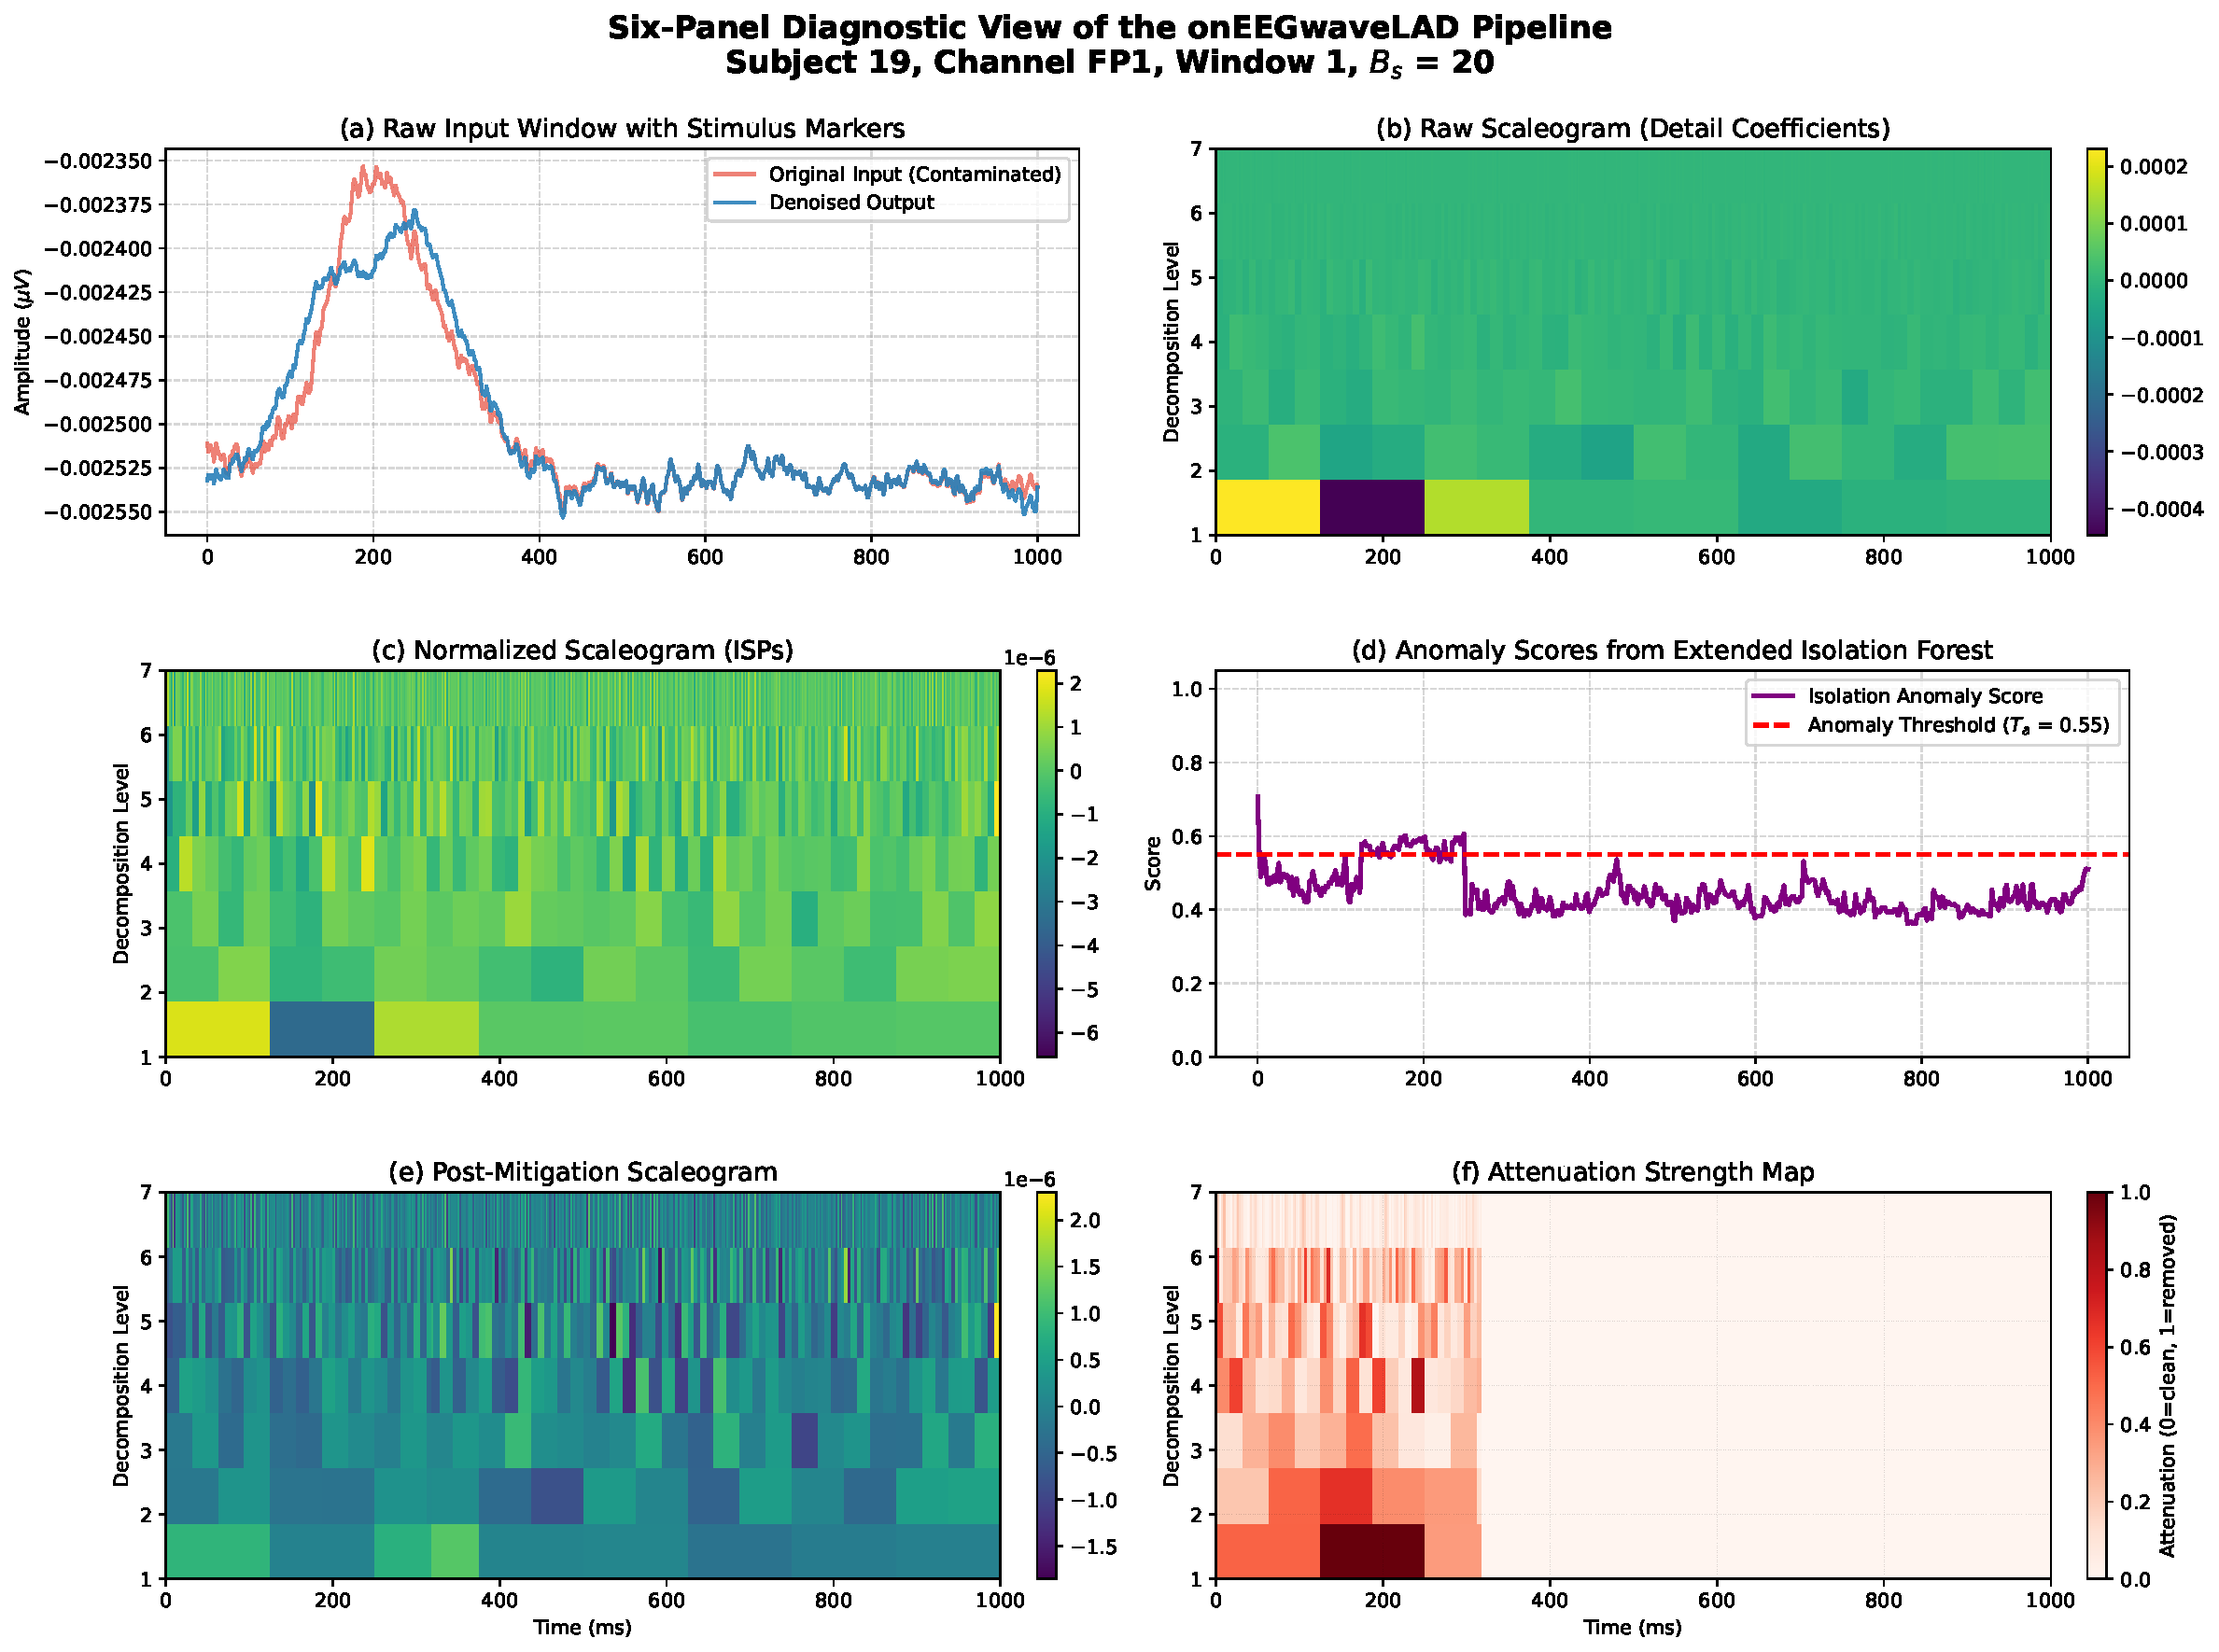
\includegraphics[width=\textwidth]{Figures/vis1_six_panel.pdf}
    \vspace{0.5em}\hrule
    \caption{Six-panel time-frequency diagnostic view of a single denoising operation on a representative window from subject 19, channel Fp1, buffer size $B_s = 8$. (a) Raw input with stimulus markers; (b) raw scaleogram (concatenated detail coefficients); (c) normalised scaleogram (ISPs); (d) anomaly scores with threshold $T_a = 0.55$; (e) post-mitigation scaleogram; (f) mitigation array (attenuation factors). The progression demonstrates selective attenuation of high-amplitude low-frequency artefacts without over-smoothing.}
    \label{fig:vis1_six_panel}
    \vspace{0.5em}\hrule
\end{figure}

\textbf{Visualisation 2: Buffer evolution over a sequence of windows.} The second diagnostic visualises the sliding buffer mechanism by presenting the population of Instantaneous Spectral Profiles as a temporal heatmap that evolves as successive windows are ingested (Figure~\ref{fig:vis2_buffer_evolution}, with animated sequence available in the appendix). Each frame corresponds to one window in the continuous recording; the vertical axis displays the $B_s$ most recent ISPs retained in the buffer (rows represent historical samples, with the current window at the top and older profiles below), and the horizontal axis spans the scaleogram feature dimensions derived from the wavelet decomposition. The heatmap intensity encodes the normalised amplitude of each feature, so that clean cortical epochs appear as relatively uniform low-intensity patterns, whereas artefactual windows introduce bright high-amplitude bands that stand out against the baseline. As the buffer advances through the recording, contaminated profiles enter at the top, persist for $B_s$ steps, and then slide out as they are displaced by newer data, allowing the detector's notion of normality to track the non-stationary structure of the signal. This temporal visualisation illustrates the consequence of buffer depth: a shallow buffer ($B_s \in \{1, 2\}$) discards the stable baseline before the detector can learn it, replacing the reference population entirely with each new window, while a sufficiently deep buffer ($B_s \geq 8$) retains enough history to distinguish transient artefacts from the variability of legitimate neural activity.

\begin{figure}[!htb]
\hrule\vspace{0.5em}
    \centering
    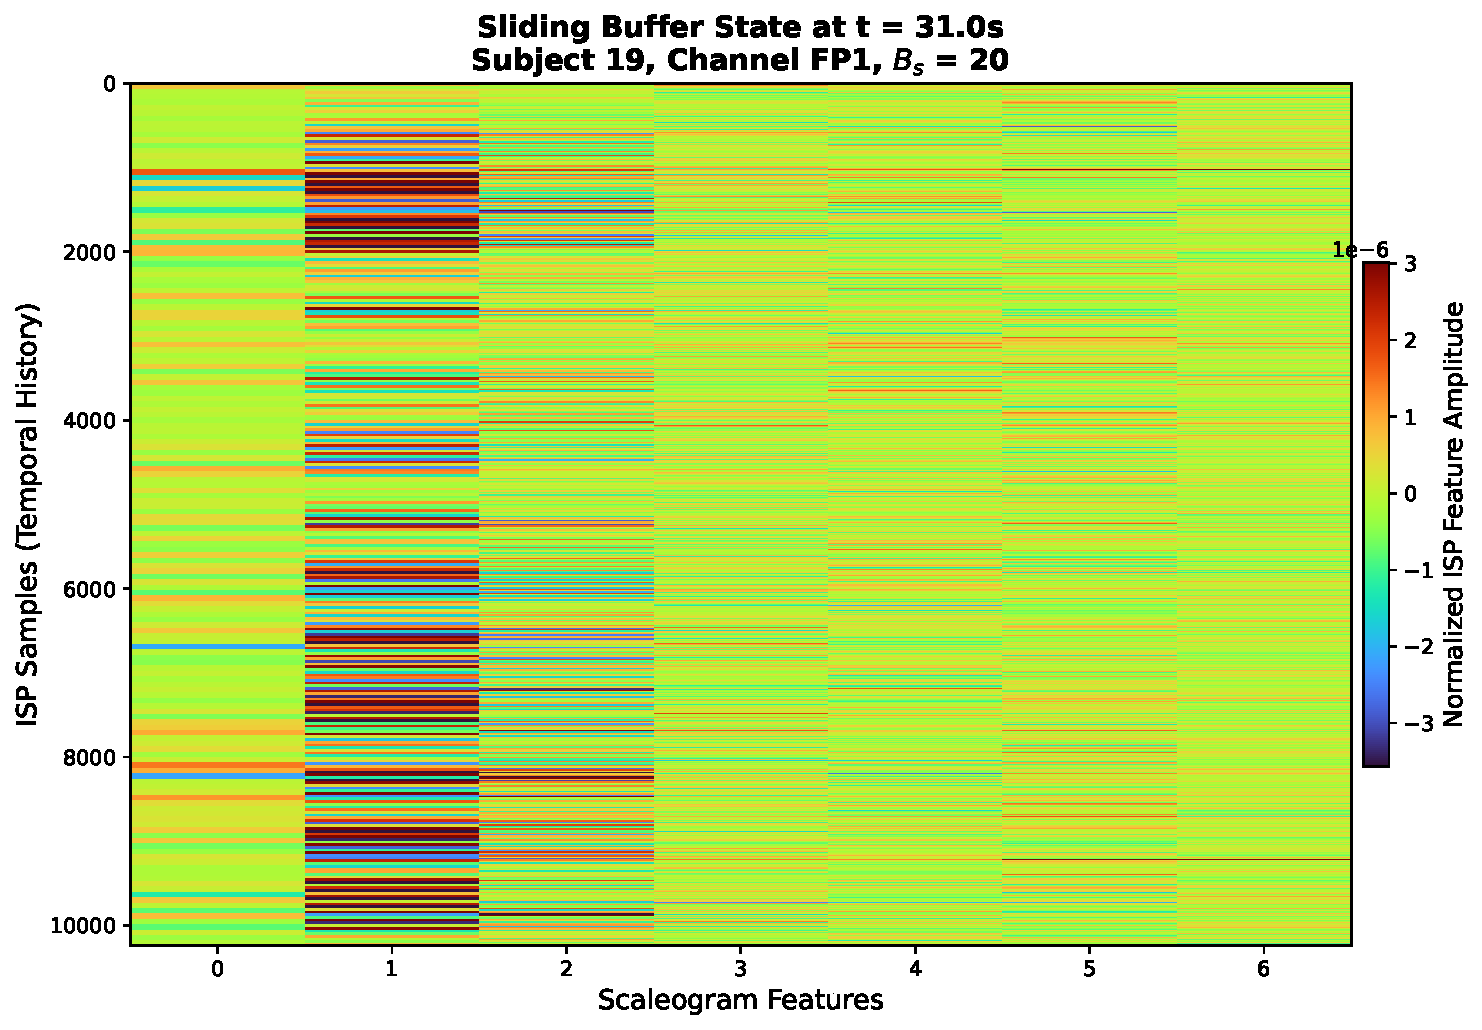
\includegraphics[width=\textwidth]{Figures/vis2_buffer_evolution.pdf}
    \vspace{0.5em}\hrule
    \caption{Sliding buffer evolution visualised as a temporal heatmap at a representative mid-sequence time point (subject 19, channel Fp1, $B_s = 8$, $t \approx 60$~s). Rows represent the $B_s$ most recent ISPs held in the buffer, with the current window at the top and older profiles below; columns span the scaleogram feature dimensions. Heatmap intensity encodes normalised feature amplitude (magma colourmap: dark = low, bright = high). Clean epochs yield relatively uniform low-intensity patterns; contaminated epochs introduce bright high-amplitude bands. Animated sequence showing the full temporal evolution is available in the appendix.}
    \label{fig:vis2_buffer_evolution}
    \vspace{0.5em}\hrule
\end{figure}

\textbf{Visualisation 3: Three-dimensional PCA projection of anomaly separation.} To verify that the threshold $T_a = 0.55$ achieves effective separation between normal and anomalous ISPs, the third diagnostic projects the scaleogram columns of a representative window into three principal components and colours each point according to whether its anomaly score exceeds $T_a$ (Figure~\ref{fig:vis3_pca_separation}). Inliers (green) form a compact cloud in the low-dimensional embedding, while outliers (red) occupy the periphery, demonstrating that the Extended Isolation Forest successfully leverages the high-dimensional wavelet representation to distinguish contaminated spectral profiles from nominal ones. The clarity of this separation confirms that the chosen threshold strikes a reasonable balance, neither so permissive that artefacts are retained nor so stringent that legitimate neural fluctuations are misclassified.

\begin{figure}[!htb]
\hrule\vspace{0.5em}
    \centering
    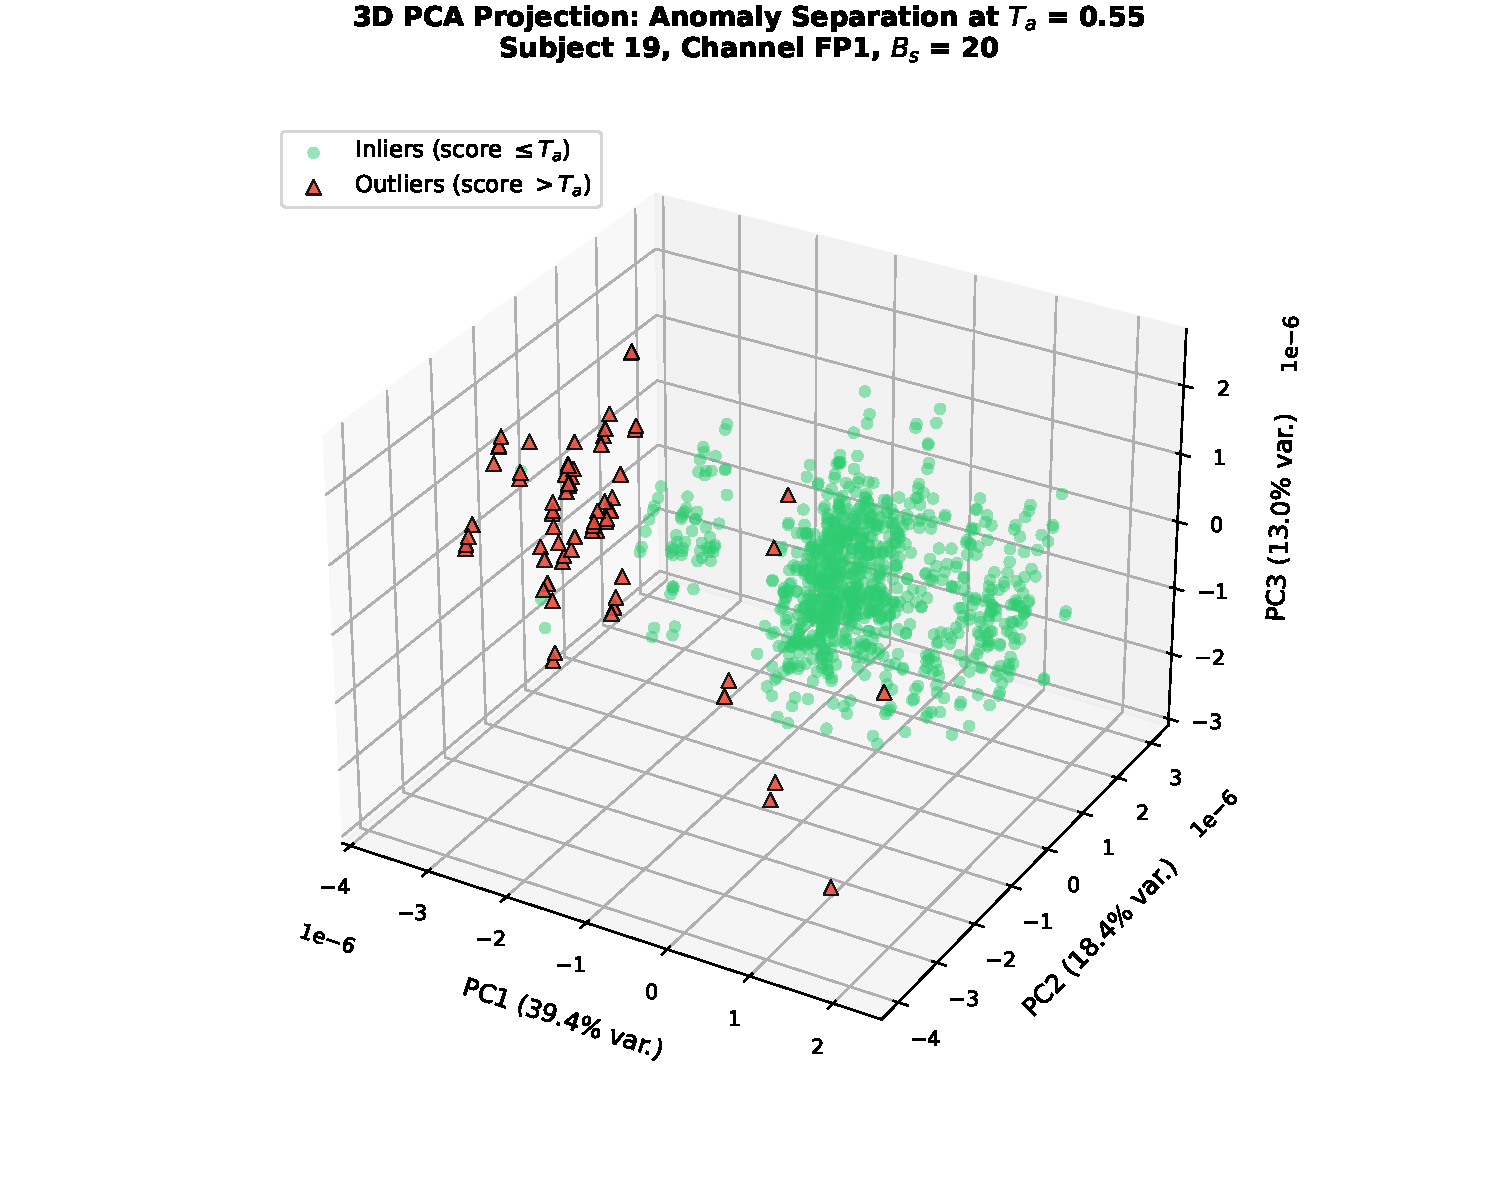
\includegraphics[width=\textwidth]{Figures/vis3_pca_separation.pdf}
    \vspace{0.5em}\hrule
    \caption{Three-dimensional PCA projection of scaleogram columns from a representative window (subject 19, channel Fp1, $B_s = 8$). Inliers (green circles, anomaly score $< T_a$) cluster compactly; outliers (red triangles, score $\geq T_a$) occupy the periphery. The three components jointly account for $70.8\%$ of variance (PC1: $39.4\%$, PC2: $18.4\%$, 
PC3: $13.0\%$). Clear separation validates the $T_a = 0.55$ threshold.}
    \label{fig:vis3_pca_separation}
    \vspace{0.5em}\hrule
\end{figure}

\textbf{Visualisation 4: Anomaly score trajectory over time.} The fourth diagnostic plots the anomaly score of each window in a continuous recording as a time series (Figure~\ref{fig:vis4_anomaly_trajectory}), with the anomaly threshold $T_a = 0.55$ marked as a horizontal reference and the score range partitioned into a clean zone (green shading below $T_a$) and a contaminated zone (red shading above $T_a$). Peaks in the anomaly score correspond to epochs in which the frontal channels exhibit extreme amplitude deviations characteristic of eye movements, while the baseline score during relatively clean segments remains well below $T_a$. This alignment between the unsupervised scoring and the observable contamination timing provides qualitative confidence that the isolation mechanism is capturing genuine physiological interference rather than arbitrary spectral variance.

\begin{figure}[!htb]
\hrule\vspace{0.5em}
    \centering
    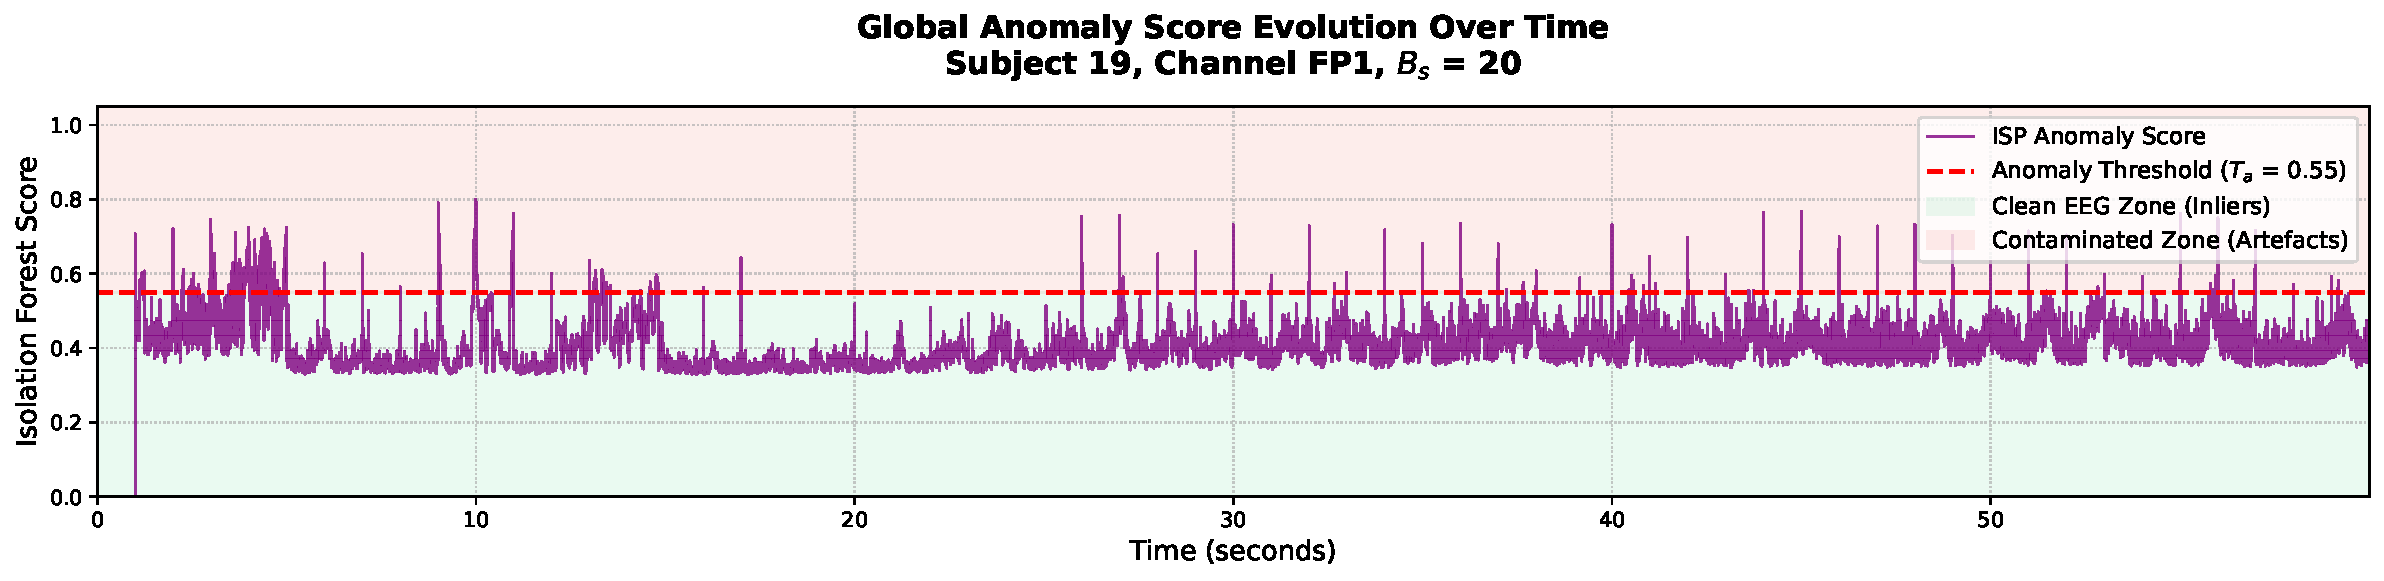
\includegraphics[width=0.95\textwidth]{Figures/vis4_anomaly_trajectory.pdf}
    \vspace{0.5em}\hrule
    \caption{Anomaly score trajectory over a continuous segment of recording (subject 19, channel Fp1, $B_s = 8$). Horizontal dashed line marks threshold $T_a = 0.55$. Green shading indicates the clean zone (scores below $T_a$); red shading indicates the contaminated zone (scores above $T_a$). Score peaks align with epochs of observable high-amplitude frontal contamination; baseline remains below threshold during clean intervals.}
    \label{fig:vis4_anomaly_trajectory}
    \vspace{0.5em}\hrule
\end{figure}

\textbf{Visualisation 5: Distribution of anomaly scores under clean versus contaminated conditions.} The final diagnostic contrasts the distribution of anomaly scores during buffer states judged to be relatively clean (the time point at which the maximum score within the buffer is minimised) against buffer states heavily contaminated by ocular activity (the time point at which the maximum score within the buffer is maximised) (Figure~\ref{fig:vis5_score_distribution}). The clean distribution is narrow and centred well to the left of $T_a$, indicating that the majority of ISPs in a clean buffer are classified as inliers, while the contaminated distribution exhibits a long right tail that crosses $T_a$ and extends into the flagged region, indicating that artefactual ISPs are correctly assigned elevated scores. This separation demonstrates that the Extended Isolation Forest is sensitive to the presence of artefacts and that $T_a = 0.55$ lies at a sensible decision boundary. The presence of some overlap between the two distributions is expected, given that the distinction between signal and noise in real EEG is not absolute, and underscores the importance of the buffer depth in stabilising this boundary: a shallow buffer yields a less reliable baseline, which would widen the clean distribution and increase misclassification, whereas a sufficiently deep buffer tightens the inlier cluster and sharpens the separation.

\begin{figure}[!htb]
\hrule\vspace{0.5em}
    \centering
    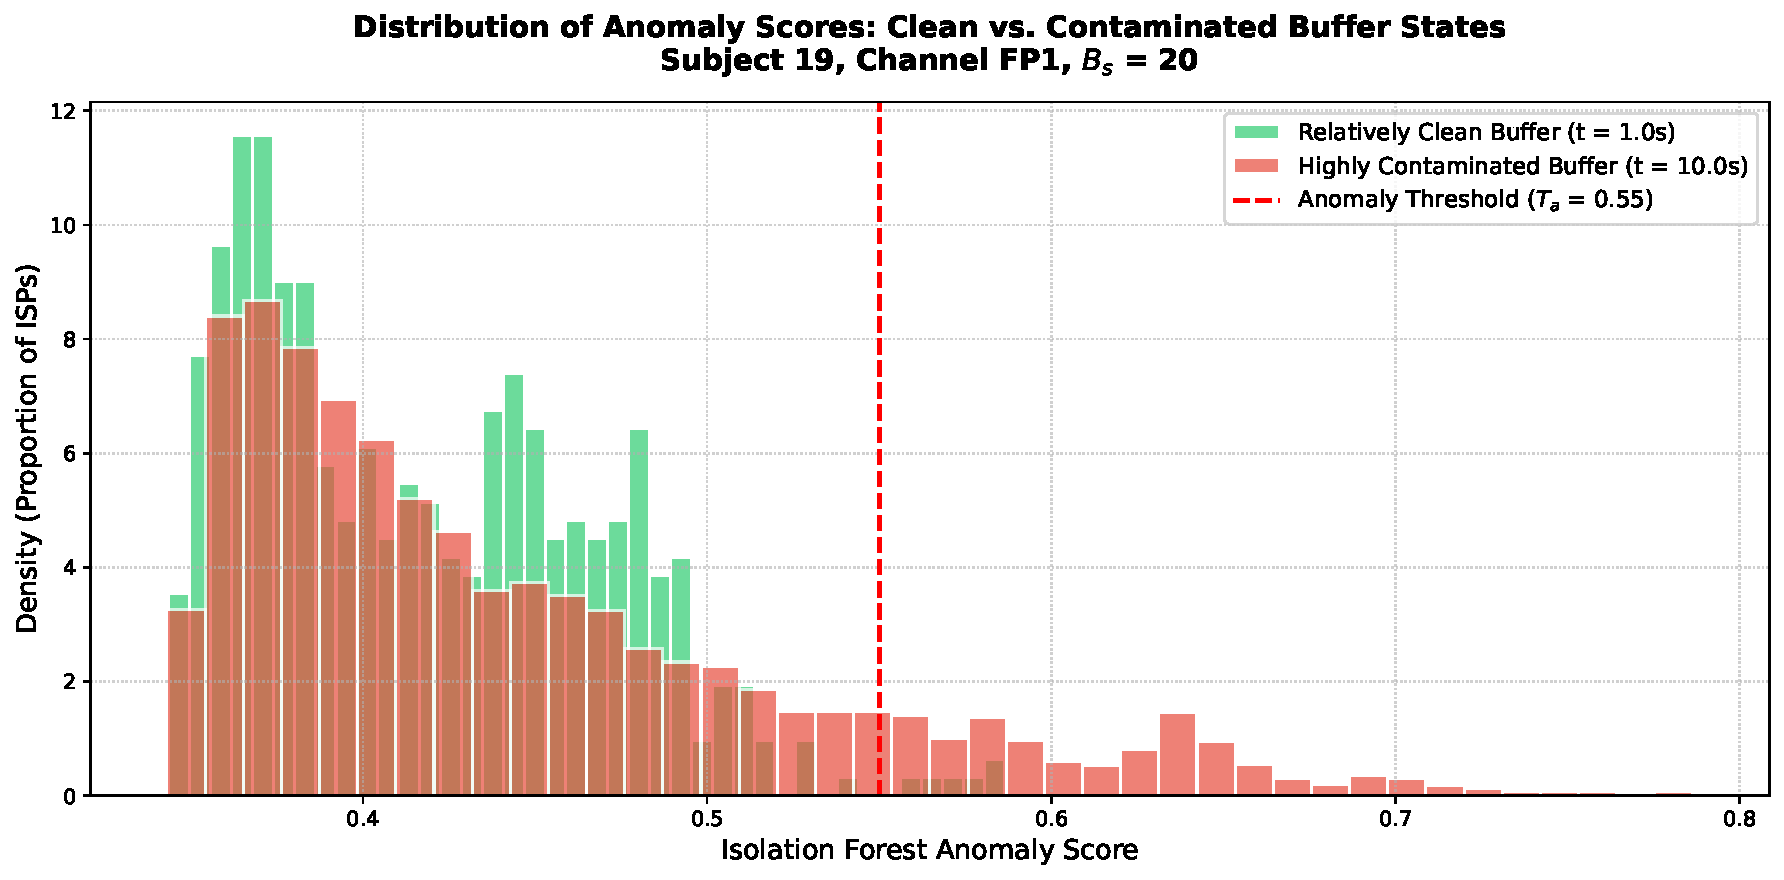
\includegraphics[width=0.85\textwidth]{Figures/vis5_score_distribution.pdf}
    \vspace{0.5em}\hrule
    \caption{Histogram comparison of anomaly scores under clean (green, buffer state at $t = t_{\text{clean}}$ when maximum score is minimised) versus contaminated (red, buffer state at $t = t_{\text{contam}}$ when maximum score is maximised) conditions, extracted from subject 19, channel Fp1, $B_s = 8$. Vertical dashed line marks $T_a = 0.55$. Clean buffer state exhibits a narrow distribution centred below threshold; contaminated buffer state exhibits a long right tail extending above threshold. This separation validates the detector's sensitivity to artefact presence.}
    \label{fig:vis5_score_distribution}
    \vspace{0.5em}\hrule
\end{figure}

Taken together, these five qualitative visualisations confirm that the onEEGwaveLAD pipeline operates as intended under the final preprocessing protocol (denoising followed by average re-referencing, with [::repeats] reconstruction), that the anomaly threshold is appropriately calibrated, and that the buffer mechanism supplies the temporal context necessary for robust artefact detection. The quantitative grid search reported in the following sections builds upon this qualitative foundation to establish at which buffer depth this behaviour converges to a stable, competitive level of performance.

\section{Modeling Outcomes: Buffer Size and Baseline Denoising}
\label{sec:modeling_results}


The modeling phase examines buffer size effects and baseline method performance through two parallel analyses. The first dissects the behaviour of the fifteen evaluation metrics across the buffer size grid, revealing fundamental directional divergences between similarity-oriented and artefact-removal indicator families and identifying where convergence occurs, while the second documents the outcomes of five automated baseline methods under identical experimental conditions to establish the competitive landscape against which the convergence lower bound must be interpreted.

    \subsection{Impact of Adaptive Buffer Size: Indicator Family Analysis}
\label{subsec:impact_bs}

The fifteen evaluation metrics, though all nominally assessing denoising quality, exhibit fundamentally different directional preferences that reflect distinct operational goals. This heterogeneity has profound implications for how the metrics should be aggregated and interpreted, and must be made explicit before the convergence lower bound can be located. Accordingly, the metrics are organised into two principal categories, whose behaviours across the buffer size grid reveal complementary aspects of the trade-off between signal preservation and artefact removal.

\textbf{The similarity-oriented category}, comprising ten metrics (Pearson correlation, mutual information, root mean squared error, the five band power preservation errors, and magnitude squared coherence in the alpha and beta bands only), measures the structural fidelity of the denoised signal relative to the original recording. To assess convergence behaviour robustly, the metric trajectories were analysed using two complementary aggregation methods: arithmetic mean aggregation (treating all ten similarity-oriented metrics with equal weight) and median aggregation (insensitive to outlier influence from extreme values). Both methods yielded consistent monotonic convergence patterns, with the median serving as a stability check against the influence of tail behaviour in individual metrics. These metrics treat the input as a reference to be preserved, so that aggressive modification--even if it removes genuine artefacts--is penalised as a loss of waveform agreement. Across the thirty subjects and thirty channels, every member of this category exhibits a monotonically improving trajectory as $B_s$ increases from $1$ to $64$: correlation and mutual information rise, RMSE and band power errors decline, and alpha/beta coherence strengthens. The improvement is steepest over the range $B_s \in \{1, 2, 4\}$, where the shallow buffer forces the detector to operate on minimal historical context, and then levels off as the buffer deepens, approaching a noise floor beyond which further enlargement yields diminishing marginal returns. Physically, this behaviour reflects the stabilisation of the Extended Isolation Forest's decision boundary as the volume of baseline material grows; with a richer history, the detector better distinguishes transient artefacts from legitimate neural variability, applying attenuation more conservatively and preserving more of the original structure.

\textbf{The artefact-removal category}, in contrast, comprises five metrics: the differences in signal-to-noise ratio and peak signal-to-noise ratio ($\mathrm{SNR}_{\mathrm{diff}}$ and $\mathrm{PSNR}_{\mathrm{diff}}$), plus magnitude squared coherence in the theta, gamma, and delta bands (MSC theta/gamma/delta). All five quantify aspects of contamination suppression rather than waveform preservation. Unlike the similarity metrics, which are agnostic to whether the preserved structure is signal or noise, these five metrics explicitly reward the removal of contamination. The inclusion of MSC theta, gamma, and delta in this category reflects their observed directional alignment with SNR-Diff and PSNR-Diff: unlike MSC alpha and beta, which improve monotonically with buffer depth and align with the similarity-oriented majority, these three frequency bands exhibit the same preference for aggressive small-buffer attenuation. Their trajectories across the buffer grid are non-monotonic: all five favour \emph{smaller} buffers, peaking in the range $B_s \in \{1, 2, 4\}$ where the aggressive attenuation applied by an undertrained detector removes more artefactual energy, and then declining at larger $B_s$ as the detector's conservative behaviour preserves more of the baseline contamination. This decline is not evidence that large buffers degrade denoising quality in an absolute sense, but rather that the artefact-removal metrics are structurally biased toward aggressive pruning, which is antithetical to the signal-preservation goal that dominates the majority of the metric suite.

The divergence between these two categories has a critical methodological consequence: aggregating all fifteen metrics through a simple mean yields a composite trajectory that exhibits an artificial rebound at large $B_s$, driven entirely by the upward slope of the five artefact-removal metrics as they move away from their small-buffer optima. This rebound is not a unified real effect reflecting a common degradation mechanism, but rather a mathematical artefact of mixing indicators with opposing directional preferences. Treating the mean trajectory as a primary basis for identifying the convergence lower bound would therefore be misleading, since it conflates the levelling-off of the similarity-oriented majority with the countervailing movement of the artefact-removal minority.

An additional complication arises from the extreme tail behaviour of $\mathrm{SNR}_{\mathrm{diff}}$. Inspection of the raw metric values across the thirty subjects reveals that approximately $0.70\%$ of channel--subject--buffer combinations (44 observations out of 6,300 total) yield catastrophically negative SNR differences, with magnitudes exceeding $-10$~dB and the most extreme value reaching $-91.8$~dB (Table~\ref{tab:snr_diff_tail}). These outliers occur exclusively at the smallest buffer sizes ($B_s \in \{1, 2\}$) and are concentrated in individual channels where the undertrained detector over-trims the signal, collapsing the stimulus-locked response and inflating the relative noise floor. Crucially, these catastrophic negatives are not the result of numerical saturation: the signal-to-noise computation employs a safety cap of $\pm 100$~dB to guard against division-by-zero edge cases, but this cap is triggered in fewer than $0.59\%$ of observations (37 cases reaching $|\mathrm{SNR}_{\mathrm{diff}}| \geq 80$~dB, all negative, and none exceeding the $\pm 100$ limit). The tail behaviour is therefore a genuine property of the metric under extreme attenuation, not an artefact of the implementation. The presence of this long negative tail, however, renders the mean aggregation unstable: a single catastrophic outlier can dominate the average across subjects, distorting the apparent trend. This instability provides an empirical justification for adopting a robust aggregator-either the median, which is insensitive to tail extremes, or category-stratified analysis, which isolates the artefact-removal metrics so that their non-monotonic behaviour does not contaminate the convergence assessment of the similarity-oriented majority.

\begin{table}[!htb]
    \centering
    \begin{tabular}{lrrr}
        \toprule
        \textbf{Metric} & \textbf{Grid stage} & \textbf{Range (dB)} & \textbf{Extreme tail ($|$value$| \geq 10$ dB)} \\
        \midrule
        \multirow{2}{*}{$\mathrm{SNR}_{\mathrm{diff}}$} 
        & Stage~1 (7 Bs) & $[-91.8, +5.0]$ & 44 obs. (0.70\%), all negative \\
        & Stage~2 (8 Bs) & $[-91.8, +3.7]$ & 44 obs. (0.61\%), all negative \\
        \midrule
        \multirow{2}{*}{$\mathrm{PSNR}_{\mathrm{diff}}$} 
        & Stage~1 (7 Bs) & $[-89.8, +7.8]$ & 1 obs. (0.02\%), negative \\
        & Stage~2 (8 Bs) & $[-3.9, +7.5]$ & 0 obs. (0.00\%) \\
        \midrule
        \multicolumn{4}{l}{\textit{Cap trigger ($|$value$| \geq 80$ dB, cap at $\pm 100$ dB):}} \\
        \multirow{2}{*}{$\mathrm{SNR}_{\mathrm{diff}}$} 
        & Stage~1 & -- & 37 obs. (0.59\%), all negative \\
        & Stage~2 & -- & 36 obs. (0.50\%), all negative \\
        \multirow{2}{*}{$\mathrm{PSNR}_{\mathrm{diff}}$} 
        & Stage~1 & -- & 1 obs. (0.02\%), negative \\
        & Stage~2 & -- & 0 obs. (0.00\%) \\
        \bottomrule
    \end{tabular}
    \caption{Tail statistics for the artefact-removal metrics across both grid stages. Stage~1: thirty subjects $\times$ thirty channels $\times$ seven buffer configurations ($N = 6{,}300$ observations per metric). Stage~2: thirty subjects $\times$ thirty channels $\times$ eight buffer configurations ($N = 7{,}200$ observations per metric). Catastrophic negatives occur at small buffer sizes due to over-trimming of individual channels and are confined to the same 44 subject--channel combinations across both stages. The cap of $\pm 100$~dB is triggered in fewer than $0.6\%$ of cases in both stages, confirming that the tail behaviour is genuine rather than a numerical artefact. Observations 
are pooled across subject--channel--buffer combinations; the count reflects unique (subject, 
channel, $B_s$) triplets, with each triplet evaluated on all fifteen metrics but the tail 
statistics reported separately per metric.}
    \label{tab:snr_diff_tail}
\end{table}

As Table~\ref{tab:snr_diff_tail} confirms, the programmatic cap of $\pm 100$~dB was approached (values with $|\mathrm{SNR}_{\mathrm{diff}}| \geq 80$) in only $0.59\%$ of observations in Stage~1 and $0.50\%$ in Stage~2, and was never exceeded in either stage, establishing that the non-monotonic behaviour of the artefact-removal metrics reflects their inherent directional preference for aggressive attenuation rather than numerical saturation at the safety threshold. The catastrophic negative values documented in the table--44 observations with $\mathrm{SNR}_{\mathrm{diff}} < -10$~dB, the most extreme reaching $-91.8$~dB--are concentrated exclusively at the smallest buffer sizes ($B_s \in \{1, 2\}$) and arise from over-trimming in individual channels where the undertrained detector collapses the stimulus-locked response. This tail behaviour provides direct empirical evidence that shallow buffers starve the Extended Isolation Forest of sufficient baseline material, corroborating the convergence lower bound identified at $B_s = 8$ and justifying the use of robust aggregators such as the median to guard against the influence of these outliers on the mean-based improvement trajectories.

In light of these findings, the subsequent analyses employ category-stratified reporting when describing raw metric behaviour and median aggregation as a robustness check on the mean-based convergence assessment. The five artefact-removal metrics are acknowledged as valid components of the evaluation suite--they capture a real aspect of denoising quality--but their opposing preference for small buffers is treated as a distinct signal rather than a distortion to be corrected, and their influence on aggregate trends is isolated so that the convergence behaviour of the similarity-oriented majority can be read without confounding.

    \subsection{Identification of the Convergence Lower Bound $X$}
\label{subsec:identification_threshold}

Having established that the similarity-oriented metrics converge monotonically while the artefact-removal metrics exhibit non-monotonic behaviour, the task now is to locate the buffer size at which this convergence effectively begins--the lower bound $X$ below which denoising quality is degraded and above which further increases in buffer depth yield diminishing returns. Three complementary lines of evidence are employed to triangulate this threshold: a parameter-free elbow-detection algorithm applied to marginal improvement curves (Evidence Line 1), a rank-based definition within the non-parametric comparison framework (Evidence Line 2), and a robustness check through median aggregation (Evidence Line 3, treated as a stability verification rather than an independent confirming analysis).

\subsubsection*{Evidence Line 1: Diminishing-Returns Inflection Point via Kneedle Algorithm}

The first line of evidence derives from the rate at which denoising quality improves as the buffer size increases. For each of the fifteen metrics, the cross-subject mean trajectory was computed across the buffer grid, and a normalised marginal improvement was calculated as the relative gain per step, expressed in units of the metric's range:
\begin{equation}
    \Delta_m(B_i \to B_{i+1}) = \frac{v(B_{i+1}) - v(B_i)}{\max_B v - \min_B v},
\end{equation}
where $v(B)$ is the mean value of the metric at buffer size $B$, and the denominator normalises by the metric's full span across the grid so that improvements in metrics with different scales can be compared on a common footing. This normalisation converts each metric into a dimensionless measure of how much of its total improvement potential is realised at each step. The fifteen normalised improvement curves were then aggregated through their mean (with polarity adjusted so that positive $\Delta_m$ uniformly denotes improvement) to produce a composite trajectory reflecting the relative gain in denoising quality per unit increase in buffer size.

Because the two-stage grid employs different spacing strategies--Stage~1 ($B_s \in \{1, 2, 4, \allowbreak 8, 16, 32, 64\}$) uses exponentially spaced values plotted on a logarithmic horizontal axis, while Stage~2 ($B_s \in \{4, 6, 8, 10, 12, 14, 16, 18\}$) uses a finer linear grid--the Kneedle algorithm was applied separately to each stage to avoid conflating the effects of grid refinement with the effects of axis scaling. Stage~1 analysis (Figure~\ref{fig:lower_bound_stage1}) identifies the elbow at $B_s = 4$, where the marginal improvement curve exhibits a sharp downward inflection: the gain per step drops from approximately $0.38$ (for the transition $1 \to 2$) and $0.19$ ($2 \to 4$) to $0.15$ ($4 \to 8$), signalling that the most rapid phase of improvement has concluded. Stage~2 analysis (Figure~\ref{fig:lower_bound_stage2}), which refines the search over the interval $[4, 18]$ with near-uniform spacing on a linear axis, locates the elbow at $B_s = 8$, where the marginal improvement from $6 \to 8$ is approximately $0.12$ and the subsequent transition $8 \to 10$ yields only $0.10$, consistent with the onset of a convergence plateau. Stage~2 is treated as the more precise estimate because it samples the convergence region with higher density ($\Delta B_s = 2$ versus the coarse grid's exponential spacing) and employs a linear horizontal scale that preserves the absolute spacing between buffer sizes, whereas Stage~1's logarithmic scale compresses the visual representation of the $4 \to 8$ transition and pushes the detected elbow leftward.

The shift in the identified elbow from $B_s = 4$ (Stage~1) to $B_s = 8$ (Stage~2) arises from two factors: first, the finer grid resolution in Stage~2 reveals structure that the coarse grid obscures, and second, the Kneedle algorithm is sensitive to the curvature of the plotted trajectory, which depends on the horizontal axis scale. On a logarithmic axis, the transition $4 \to 8$ occupies the same visual span as $1 \to 2$ or $2 \to 4$, compressing the appearance of the improvement curve and pushing the detected elbow leftward; on a linear axis, the $4 \to 8$ span is visually larger, and the algorithm identifies $B_s = 8$ as the point where the curve's slope diminishes most sharply. Both findings are valid within their respective presentations, but the Stage~2 result, derived from a denser grid and a scale that preserves the absolute spacing of buffer sizes, is treated as the more precise estimate. Accordingly, Evidence Line 1 locates the convergence lower bound at $B_s \approx 8$, the buffer size beyond which the rate of gain declines to a level consistent with diminishing returns.

\begin{figure}[!htb]
\hrule\vspace{0.5em}
    \centering
    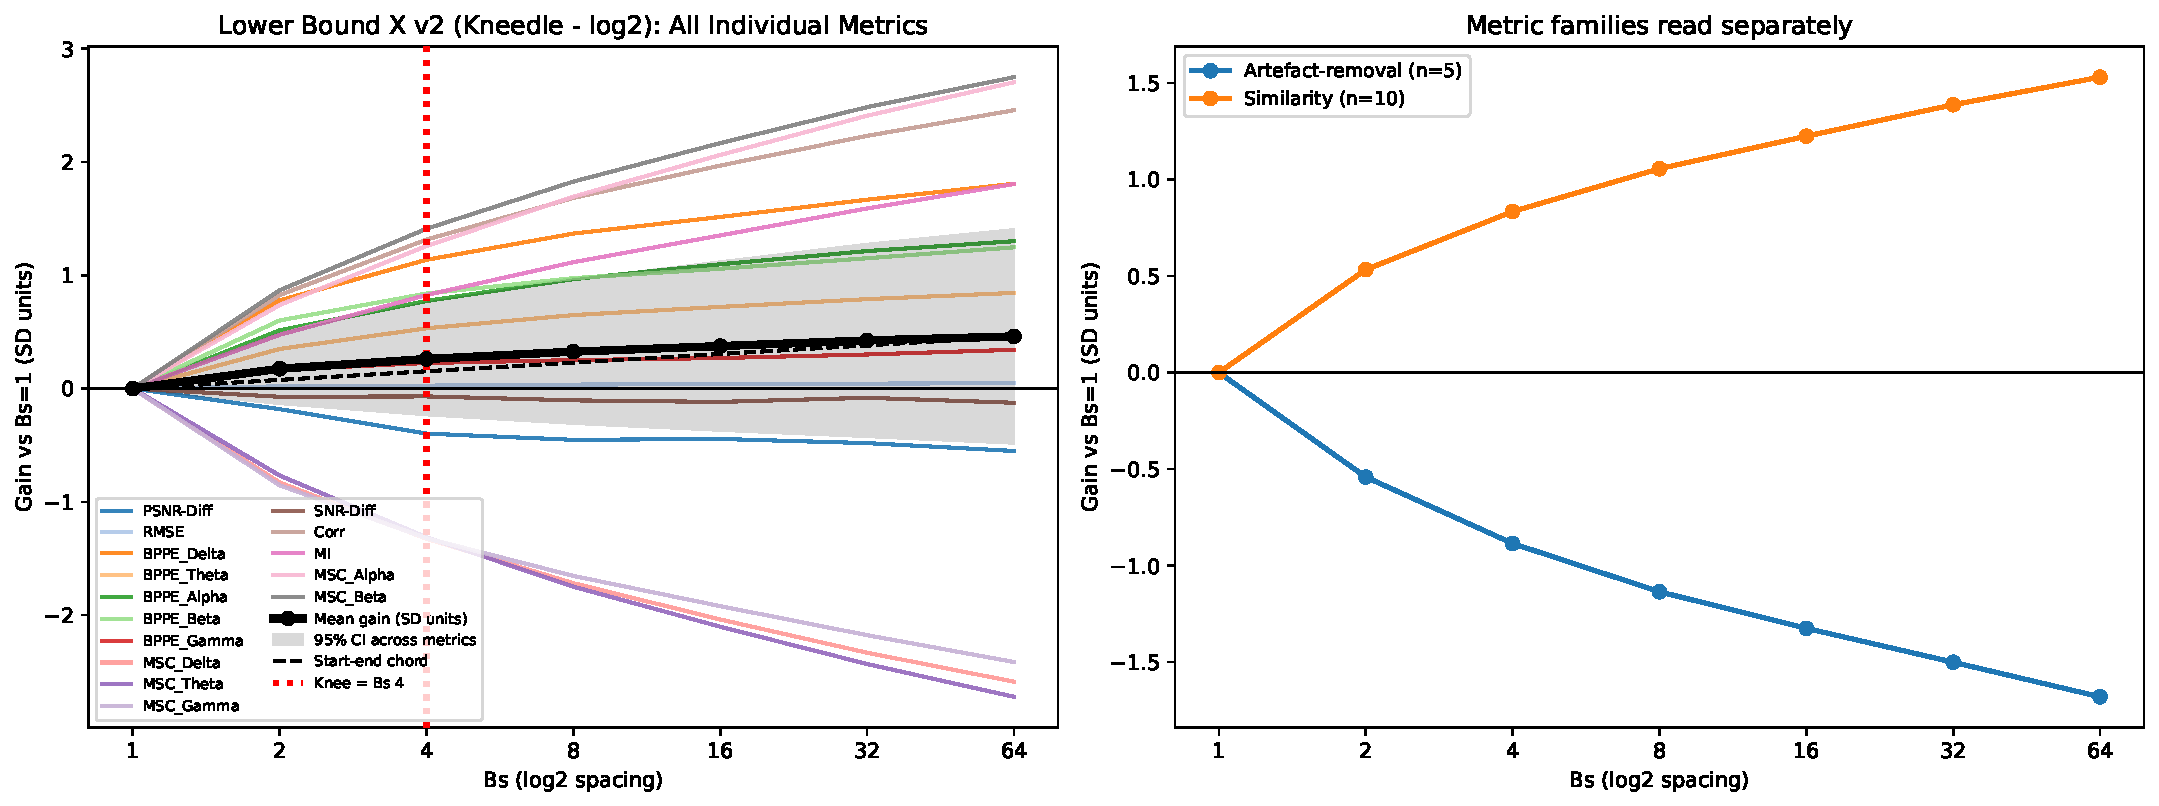
\includegraphics[width=0.9\textwidth]{Figures/lower_bound_stage1_v2.pdf}
    \vspace{0.5em}\hrule
    \caption{Stage~1 coarse-grid analysis ($B_s \in \{1, 2, 4, 8, 16, 32, 64\}$, logarithmic horizontal axis): normalised marginal improvement in denoising quality (arithmetic mean aggregation across fifteen metrics, expressed as a fraction of each metric's range) as a function of buffer size. The Kneedle algorithm identifies the elbow at $B_s = 4$, where the improvement curve exhibits a sharp downward inflection. Marginal gains continue to decline beyond $B_s = 4$, but the coarse spacing and logarithmic scale compress the visual representation; Stage~2 refines this result.}
    \label{fig:lower_bound_stage1}
    \vspace{0.5em}\hrule
\end{figure}

\begin{figure}[!htb]
\hrule\vspace{0.5em}
    \centering
    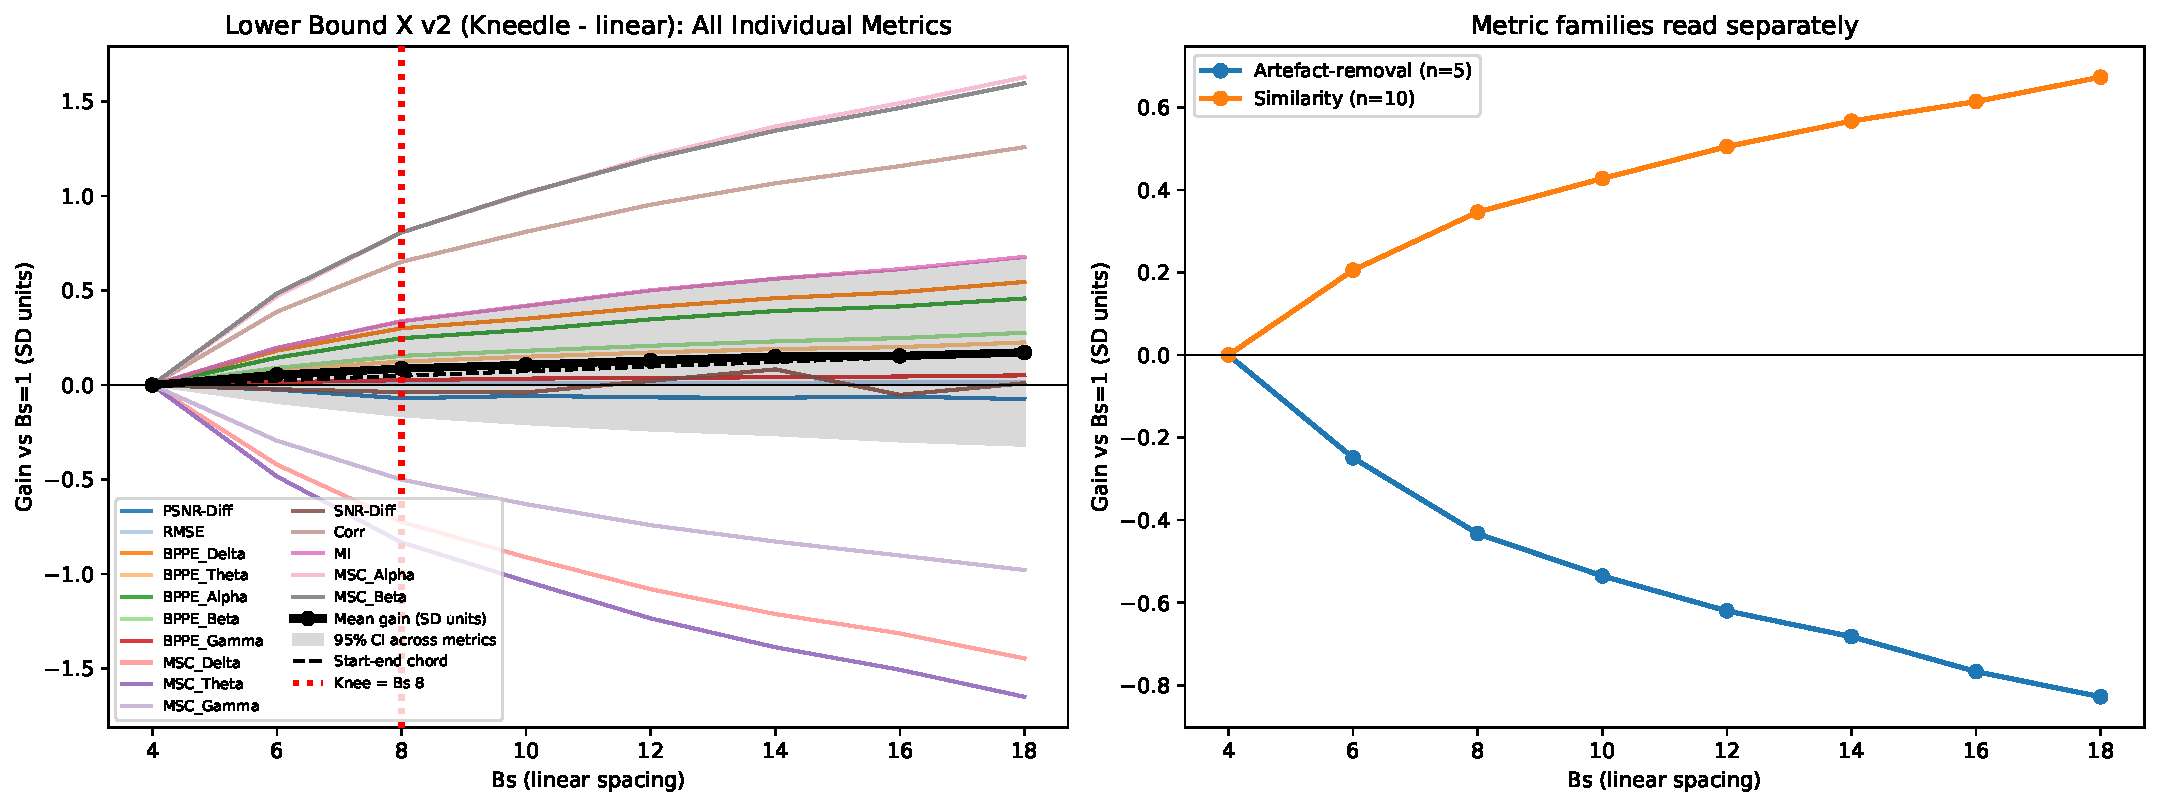
\includegraphics[width=0.9\textwidth]{Figures/lower_bound_stage2_v2_refined.pdf}
    \vspace{0.5em}\hrule
    \caption{Stage~2 refined-grid analysis ($B_s \in \{4, 6, 8, 10, 12, 14, 16, 18\}$, linear horizontal axis): normalised marginal improvement computed via arithmetic mean aggregation over the interval where the coarse grid suggested convergence was beginning. The Kneedle algorithm refines the elbow to $B_s = 8$, where the slope of the improvement curve diminishes to a level consistent with a convergence plateau. This refined estimate, derived from denser sampling and a linear scale that preserves absolute buffer spacing, is treated as the more precise location of the convergence lower bound.}
    \label{fig:lower_bound_stage2}
    \vspace{0.5em}\hrule
\end{figure}

\subsubsection*{Evidence Line 2: Rank-Based Lower Bound via Nemenyi Critical Difference}

The second line of evidence derives from the non-parametric ranking framework and provides a complementary definition of the convergence lower bound that is independent of the marginal improvement calculation. Within the subset of comparisons that include only the seven onEEGwaveLAD buffer configurations (excluding the five baseline methods), a Friedman test was performed across the thirty subjects under the channel-aggregated configuration, yielding a highly significant effect of buffer size ($\chi^2 = 177.10$, $p = 1.40 \times 10^{-35}$, $N = 30$, $k = 7$). Post-hoc analysis via the Nemenyi test established a critical difference threshold of $\mathrm{CD} = 1.163$, such that any pair of buffer sizes whose mean ranks differ by more than this value are statistically distinguishable at the $\alpha = 0.05$ level (Figure~\ref{fig:cd_bs_only}).

The rank ordering across the seven configurations is strictly monotonic, with $B_s = 64$ achieving the best mean rank ($3.098$), followed by $B_s = 32$ ($3.315$), $B_s = 16$ ($3.634$), $B_s = 8$ ($3.965$), $B_s = 4$ ($4.312$), $B_s = 2$ ($4.671$) and $B_s = 1$ ($5.004$). The Nemenyi procedure resolves this ordering into four overlapping cliques of statistically indistinguishable configurations, spanning $B_s = 64$ to $B_s = 8$, $B_s = 32$ to $B_s = 4$, $B_s = 16$ to $B_s = 2$, and $B_s = 8$ to $B_s = 1$. Within the first of these, $B_s = 8$ is the smallest buffer whose mean rank lies within the critical difference of the best-performing configuration ($|3.098 - 3.965| = 0.867 < \mathrm{CD}$), whereas $B_s = 4$ falls outside that interval ($|3.098 - 4.312| = 1.214 > \mathrm{CD}$) and is therefore separated from the plateau. Read against the operational definition adopted in Section~\ref{subsec:literature_gaps_hypotheses}, this places the rank-based lower bound at $B_s = 8$.

The overlapping structure of these cliques must be acknowledged rather than passed over, since it delimits how much weight this criterion can carry. The fourth clique groups $B_s = 8$ with $B_s = 1$, so the same test that fails to separate $B_s = 8$ from the best configuration also fails to separate it from the worst; with thirty subjects the critical difference of $1.1631$ is wide relative to the total spread of mean ranks ($1.906$ from $B_s = 64$ to $B_s = 1$), and the procedure consequently possesses limited resolution in the interior of the grid. What the analysis establishes unambiguously is an ordering and an exclusion: performance improves monotonically with buffer depth, and $B_s = 4$ and below are separated from the top of that ordering while $B_s = 8$ is not. Because the criterion cannot by itself isolate a unique threshold, it is reported as one of three converging lines of evidence rather than as a self-sufficient determination, and its agreement with the elbow analysis of Evidence Line~1 -- which operates on raw metric trajectories and is unaffected by the width of the Nemenyi interval -- is what renders the estimate at $B_s = 8$ defensible.

\begin{figure}[!htb]
\hrule\vspace{0.5em}
    \centering
    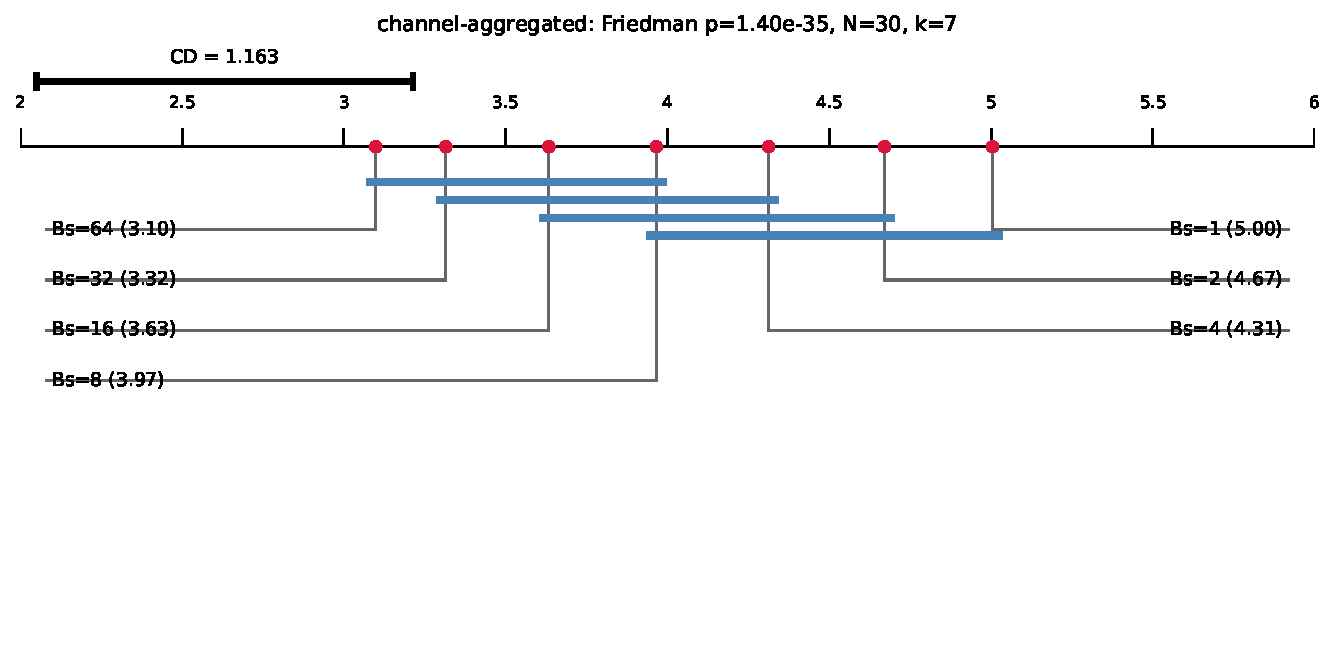
\includegraphics[width=0.85\textwidth]{Figures/CD_Bs_channel-aggregated.pdf}
    \vspace{0.5em}\hrule
    \caption{Critical difference diagram for the seven onEEGwaveLAD buffer configurations under the channel-aggregated configuration (Friedman $p = 1.40 \times 10^{-35}$, $N = 30$ subjects, $k = 7$ methods, $\mathrm{CD} = 1.163$). Configurations connected by a horizontal bar are statistically indistinguishable at the $\alpha = 0.05$ level. $B_s = 8$ (mean rank $3.97$) is the smallest buffer that lies within the critical difference interval of the best-performing buffer ($B_s = 64$, mean rank $3.10$), while $B_s = 4$ (mean rank $4.31$) falls outside this interval, indicating that performance at $B_s = 8$ has converged to the plateau attained by larger buffers.}
    \label{fig:cd_bs_only}
    \vspace{0.5em}\hrule
\end{figure}

\subsubsection*{Evidence Line 3: Median Aggregation as a Robustness Check}

The third line of evidence revisits the convergence assessment using median aggregation rather than mean aggregation, which guards against the influence of the outlier-prone artefact-removal metrics and the catastrophic negatives documented in Section~\ref{subsec:impact_bs}. It is important to note at the outset that this robustness check is \emph{not} an independent third line of evidence: because the fifteen metrics comprise ten similarity-oriented indicators and five artefact-removal indicators, the median is dominated by the similarity-oriented majority and effectively recapitulates that category's convergence behaviour rather than providing an independent synthesis of all fifteen metrics on equal terms. Its value lies in demonstrating that the convergence conclusion remains stable under a robust aggregator that suppresses outlier influence, as detailed below and discussed further in Section~\ref{sec:interpretation_findings}. For each buffer transition, the absolute value of the normalised improvement $|\Delta_m|$ was computed for all fifteen metrics, and the median of these fifteen values was taken as the representative improvement at that step. Unlike the mean, which can be dominated by a small number of extreme values, the median reflects the behaviour of the majority: if most metrics are levelling off, the median will be low, regardless of whether one or two outlier metrics exhibit continued large changes.

Across both Stage~1 and Stage~2, the median aggregation yields trajectories that are monotonically decreasing and free of the rebound observed in the mean aggregation (Figures~\ref{fig:convergence_stage1} and~\ref{fig:convergence_stage2}). In Stage~1, the median $|\Delta_m|$ drops from approximately $0.40$ at the transition $1 \to 2$ to roughly $0.10$ at $8 \to 16$, with little further decline beyond $B_s = 8$. In Stage~2, the median curve confirms this pattern: the improvement from $6 \to 8$ is approximately $0.12$, while subsequent steps ($8 \to 10$, $10 \to 12$, etc.) hover around $0.08$--$0.10$, consistent with a plateau. Both stages converge on $B_s \approx 8$ as the point beyond which the median rate of change becomes negligible, in agreement with Evidence Lines~1 and~2.

It is critical, however, to interpret this finding correctly. The median of the fifteen metrics is not an independent synthesis that weights all metrics equally; rather, it is dominated by the ten-metric similarity-oriented majority, whose monotonic convergence behaviour naturally suppresses the countervailing signal from the five artefact-removal metrics. In effect, the median aggregation is a robust re-expression of the convergence trajectory already visible in the similarity-oriented category, rather than a separate line of evidence that independently confirms the location of the lower bound. Its value lies in demonstrating that the convergence conclusion is robust to the inclusion of outlier-prone metrics: even when the five artefact-removal metrics are retained in the aggregation, the median correctly identifies the levelling-off behaviour of the ten-metric majority, whereas the mean is distorted by the artefact-removal metrics' non-monotonic tail. Evidence Line~3 is therefore treated as a stability verification rather than a third independent confirming analysis.

\begin{figure}[!htb]
\hrule\vspace{0.5em}
    \centering
    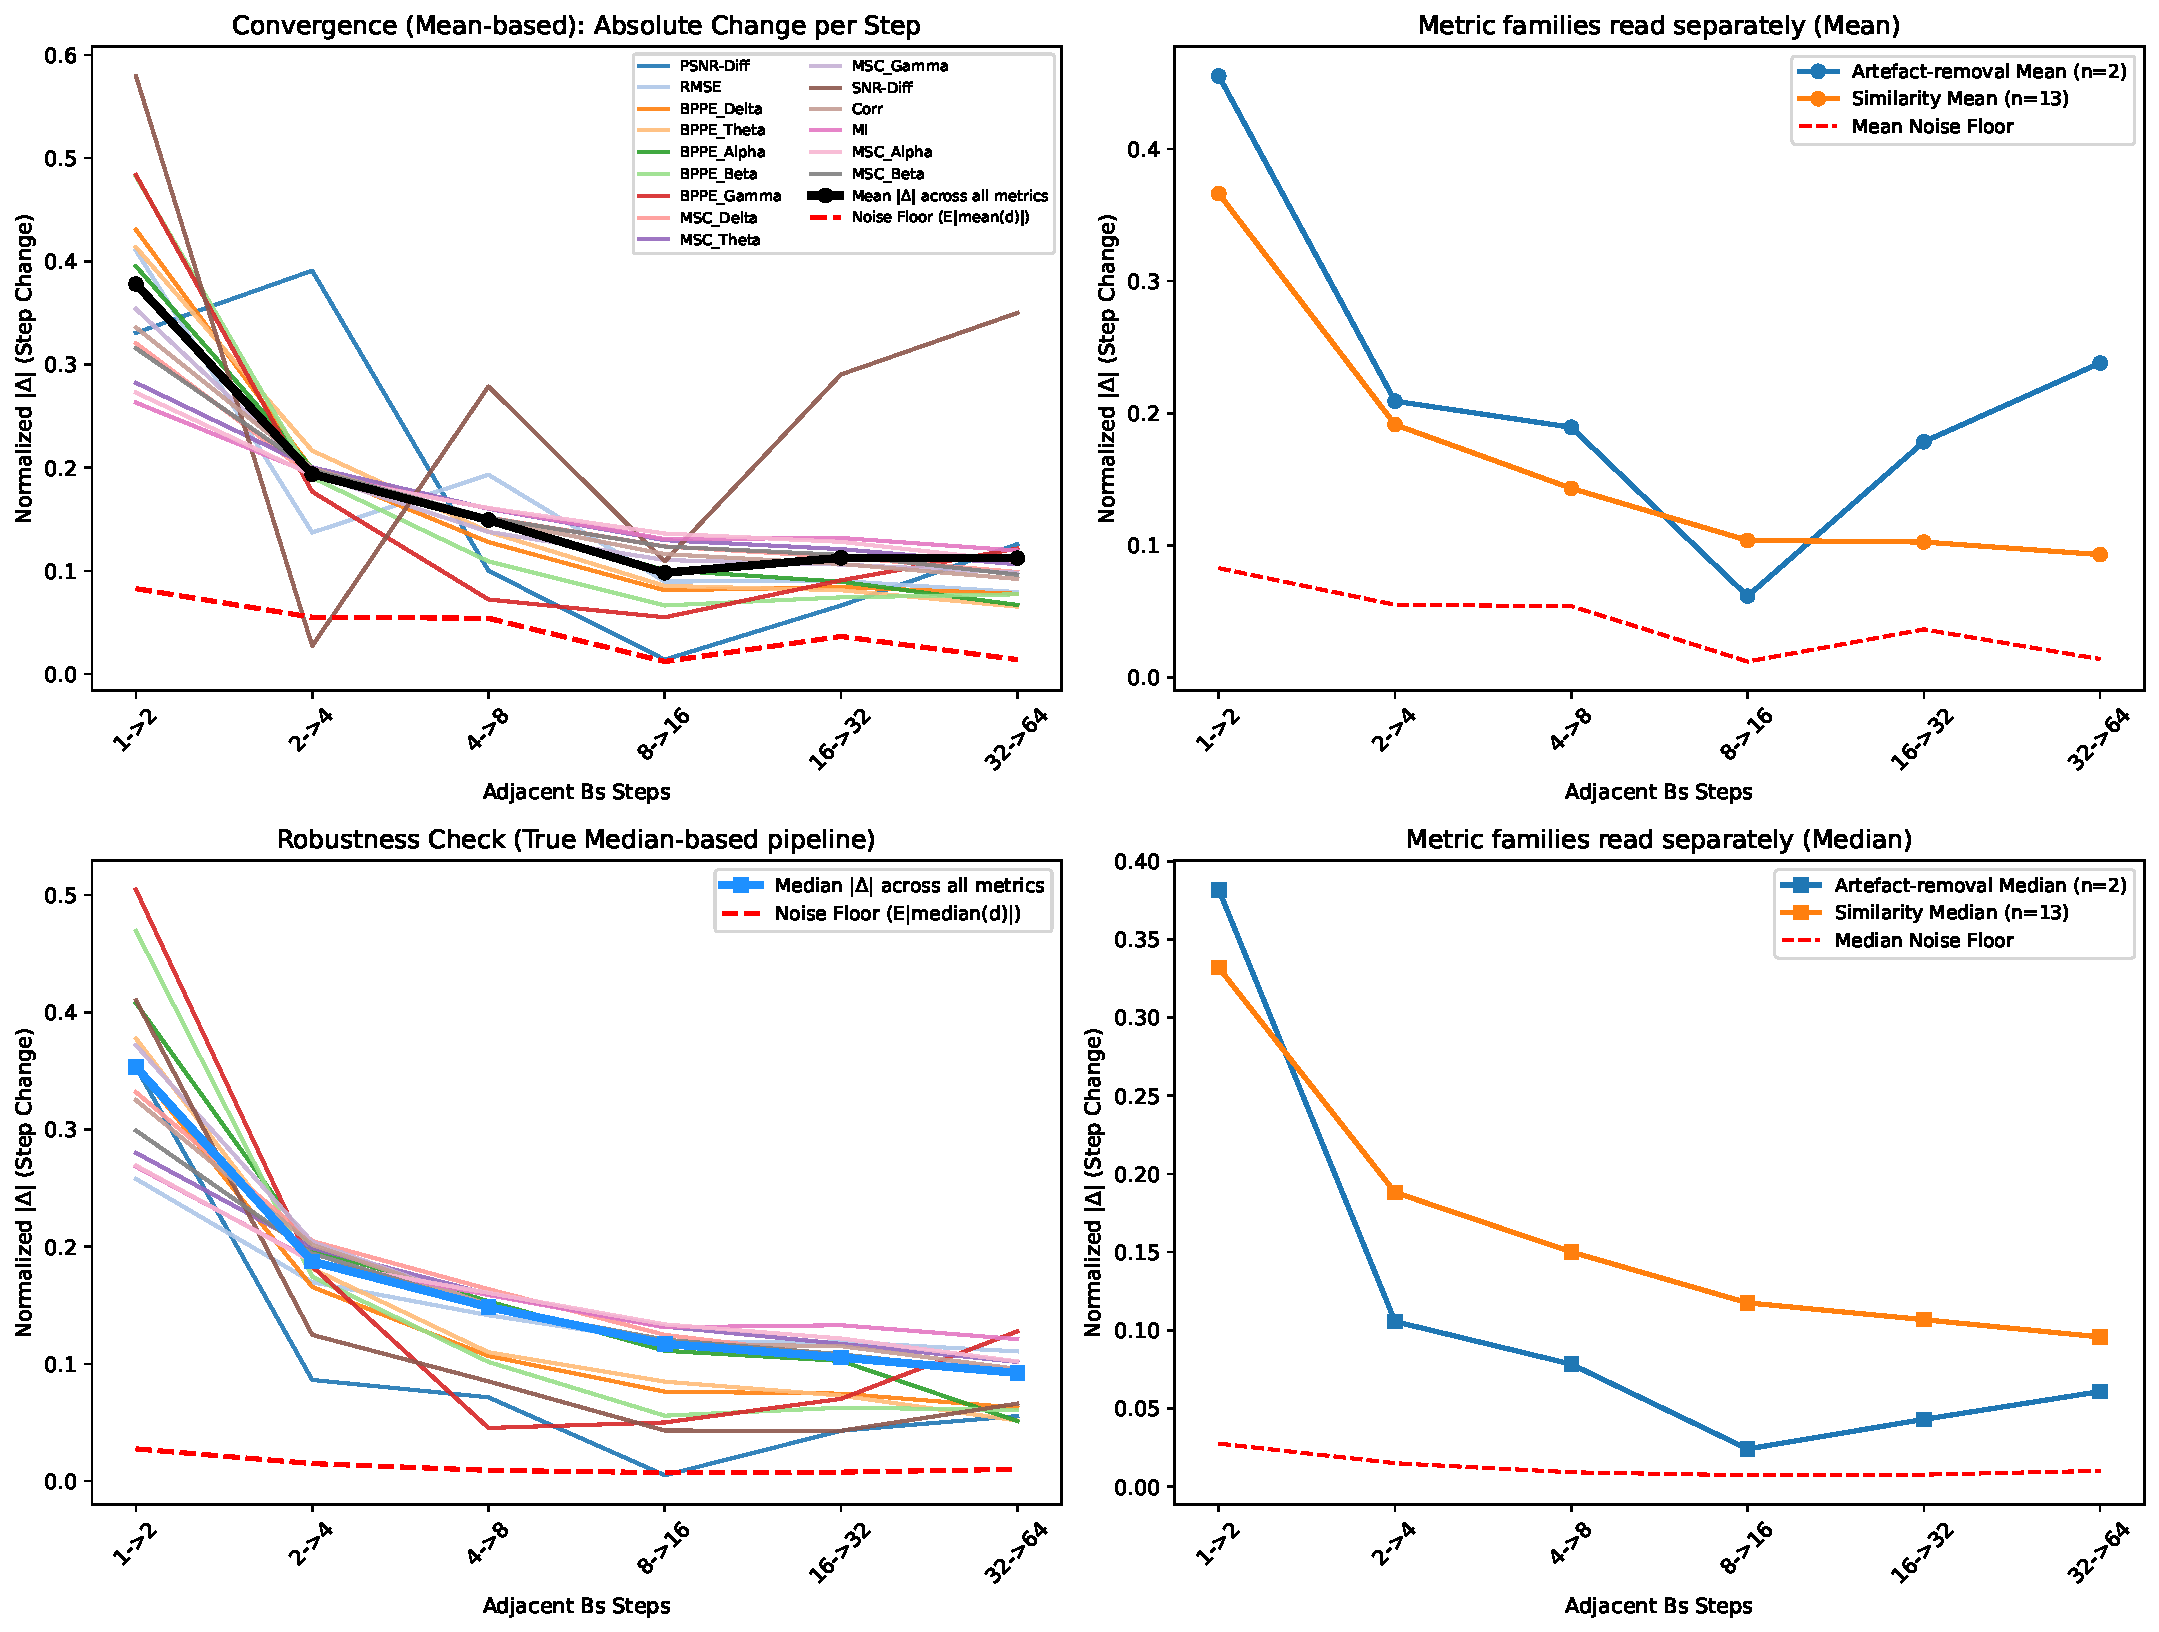
\includegraphics[width=0.9\textwidth]{Figures/convergence_stage1_v2.pdf}
    \vspace{0.5em}\hrule
    \caption{Stage~1 median aggregation: absolute value of normalised improvement, aggregated across fifteen metrics via the median. The trajectory is monotonically decreasing and converges toward a plateau beyond $B_s = 8$, with no rebound. The median is dominated by the ten similarity-oriented metrics, whose convergence behaviour it faithfully reflects, and is insensitive to the non-monotonic tail of the five artefact-removal metrics. This robustness check confirms that the convergence conclusion is not distorted by outlier influence.}
    \label{fig:convergence_stage1}
    \vspace{0.5em}\hrule
\end{figure}

\begin{figure}[!htb]
\hrule\vspace{0.5em}
    \centering
    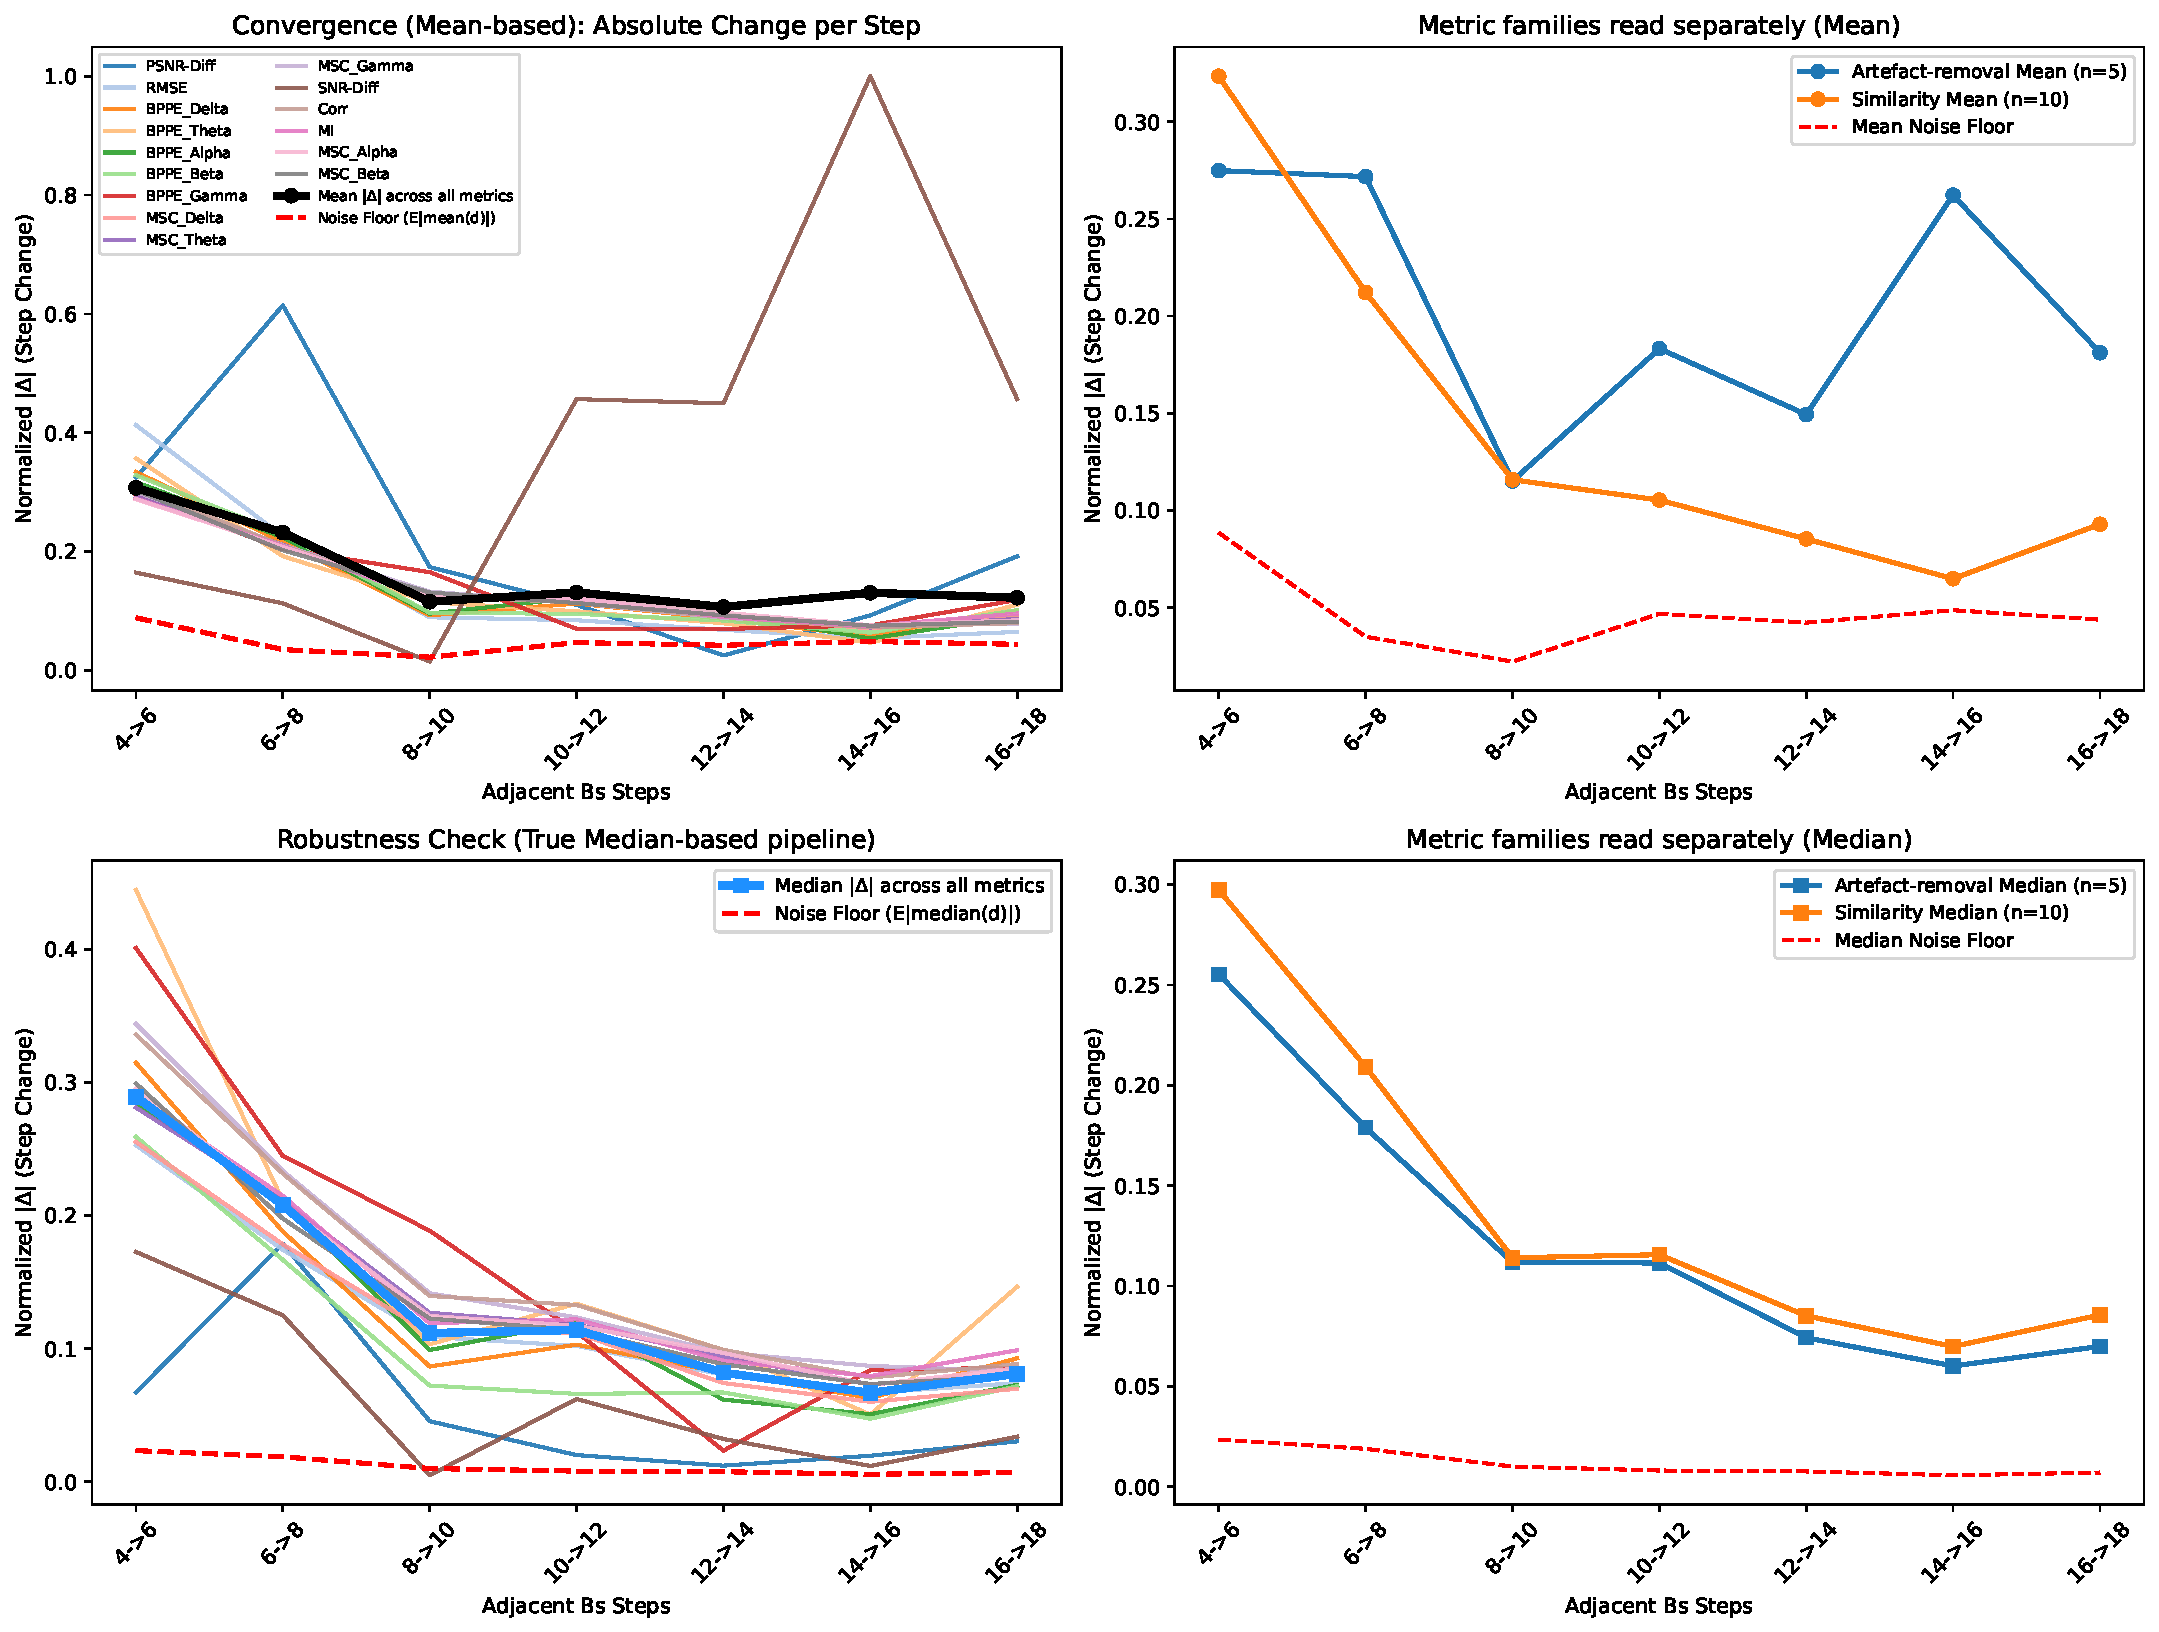
\includegraphics[width=0.9\textwidth]{Figures/convergence_stage2_v2_refined.pdf}
    \vspace{0.5em}\hrule
    \caption{Stage~2 median aggregation over the refined grid ($B_s \in \{4, 6, 8, 10, 12, 14, 16, 18\}$): the median $|\Delta_m|$ drops sharply from $B_s = 4$ to $B_s = 8$ and then levels off at approximately $0.08$--$0.10$, consistent with a convergence plateau. Both Stage~1 and Stage~2 median trajectories converge on $B_s \approx 8$, corroborating the location identified by Evidence Lines~1 and~2.}
    \label{fig:convergence_stage2}
    \vspace{0.5em}\hrule
\end{figure}

\subsubsection*{Synthesis: The Convergence Lower Bound $X \approx B_s = 8$}

The three lines of evidence converge on a consistent conclusion: the convergence lower bound for the onEEGwaveLAD framework under the final evaluation protocol lies at approximately $B_s = 8$. Below this threshold, denoising quality--as measured by the similarity-oriented metric majority--is still improving rapidly, with marginal gains per step remaining above $0.12$ (Evidence Line~1) and rank-based performance distinguishable from the best configuration (Evidence Line~2). At and beyond $B_s = 8$, the rate of improvement diminishes sharply, the rank-based performance becomes statistically indistinguishable from the plateau attained by $B_s = 64$, and the median aggregation confirms that the levelling-off behaviour is robust to the inclusion of outlier-prone metrics (Evidence Line~3).

This convergence is not absolute--larger buffers continue to yield modest incremental gains in the similarity-oriented metrics--but the diminishing returns beyond $B_s = 8$ indicate that the bulk of the denoising benefit has been realised. The practical significance of this threshold is further established by situating onEEGwaveLAD's performance at $B_s = 8$ against the five baseline methods, as reported in Section~\ref{subsec:global_performance}: $B_s = 8$ is the smallest buffer at which the framework reaches or slightly exceeds the strongest baseline, providing an independent validation that the convergence identified through internal metrics corresponds to a threshold of competitive performance in the broader denoising landscape.

    \subsection{Baseline Denoising Outcomes}
\label{subsec:baseline_outcomes}

To contextualise the onEEGwaveLAD findings within the broader landscape of automated EEG denoising, five established baseline methods were evaluated under an identical preprocessing and evaluation protocol. The baselines comprise two methodological paradigms: FASTER, a FASTER-inspired Independent Component Analysis (ICA) procedure that identifies and removes artefactual components through a suite of automated heuristics, and Artefact Subspace Reconstruction (ASR), a principal-component-based method that reconstructs contaminated segments by projecting them onto a low-dimensional subspace learned from clean calibration data. Four variants of ASR were included to span its configuration space: ASR\_offline\_13 and ASR\_offline\_20 use the entire recording for calibration with cutoff thresholds of $13$ and $20$ standard deviations, respectively, while ASR\_online\_13 and ASR\_online\_20 simulate online operation by calibrating on an initial twenty 1-second windows and applying the learned subspace to the remainder of the stream.

All five baselines were applied to signals preprocessed according to the unified protocol described in Section~\ref{sec:data_prep_streaming}: 1~Hz high-pass filtering followed by the addition of a flat reference channel and average re-referencing across the thirty EEG electrodes. This preprocessing harmonisation ensures that differences in denoising outcomes reflect the methods' algorithmic logic rather than incidental disparities in their input conditioning. The FASTER procedure employed a vertical EOG channel (VEOG\_lower) for EOG-correlation-based component rejection, applied a $z$-score threshold of $3$ across five component attributes (spatial kurtosis, slope of the log-frequency spectrum, Hurst exponent, median gradient, and EOG correlation), and reconstructed the signal after removing flagged components. The ASR variants followed the implementation detailed in Section~\ref{sec:baseline_methods}, with offline calibration incorporating a pre-cleaning step to exclude heavily contaminated epochs from the reference subspace, and online calibration restricted to the initial segment to mimic real-time deployment constraints.

The denoised outputs of all five baselines were evaluated through the same fifteen-metric suite applied to onEEGwaveLAD, yielding a uniform basis for comparison. The raw metric distributions across subjects and channels reveal that FASTER, the simplest of the five, exhibits the most conservative behaviour, removing fewer components on average and therefore preserving more of the original structure at the cost of retaining more residual artefacts; this is reflected in its high similarity-metric scores but poor artefact-removal scores. The ASR variants occupy an intermediate range: the offline configurations, which calibrate on the full recording and pre-clean the calibration data, outperform their online counterparts, while the higher cutoff threshold ($20$) yields more aggressive reconstruction than the lower threshold ($13$), translating to better artefact suppression but slightly reduced waveform fidelity. Among the five baselines, ASR\_offline\_20 emerges as the strongest performer when ranks are aggregated across the fifteen metrics, achieving the best balance between preserving neural structure and attenuating contamination.

These baseline results are not presented in isolation but are integrated into the joint twelve-method ranking that includes the seven onEEGwaveLAD buffer configurations, so that the convergence lower bound identified in Section~\ref{subsec:identification_threshold} can be interpreted in terms of its relative standing against established methods. The statistical outcomes of this joint comparison, including the Friedman test across all twelve methods and the Nemenyi critical difference diagrams that situate $B_s = 8$ against the baselines, are reported in Section~\ref{subsec:global_performance}.

\section{Evaluation Results: Joint Non-Parametric Analysis}
\label{sec:eval_results_stats}


The evaluation phase converts raw metric values into ranks and applies non-parametric statistical procedures across three complementary configurations, each varying in its treatment of within-subject and across-channel dependence. The first subsection presents the Friedman test outcomes under the three configurations and confirms directional significance through a seven-buffer monotonicity analysis, the second subsection interprets the competitive standing of the convergence lower bound relative to baseline methods through Nemenyi critical difference diagrams, and the third subsection triangulates the convergence threshold through three independent analytic procedures applied to the raw metric trajectories.

    \subsection{Friedman Test Results Across Configurations}
\label{subsec:friedman_results}

The fifteen raw metric values were converted into ranks at the channel--subject level, with each of the twelve methods (seven onEEGwaveLAD buffer configurations plus five baselines) receiving a rank from $1$ (best) to $12$ (worst) for every combination of metric, subject, and channel. These ranks were then aggregated across the fifteen metrics to produce a single mean rank per method per subject--channel pair, and submitted to Friedman tests under three complementary configurations that vary in their treatment of within-subject and across-channel dependence. The three-tier analysis strategy, formalised in Table~\ref{tab:three_tier_analysis} of Chapter~\ref{chap:methodology}, assigns distinct roles to each configuration: the baseline comparison (twelve methods jointly ranked) establishes the practical significance of the convergence lower bound by demonstrating where onEEGwaveLAD attains competitive performance, the convergence bound identification (applied to raw trajectories, reported in Section~\ref{subsec:identification_threshold}) locates the buffer size at which metric values cease to change meaningfully, and the directional significance test (seven buffer configurations only, excluding baselines) confirms that buffer size exerts a statistically significant monotonic effect.

\textbf{Configuration 1: Channel-aggregated, multiple subjects ($N = 30$, $k = 12$).} In this configuration, the thirty channels within each subject are first converted to ranks, and these ranks are averaged to produce a single representative rank per method per subject. The Friedman test is then applied across the thirty subjects, treating each subject as an independent replicate. This configuration balances statistical power against the assumption of independence by collapsing within-subject channel variation, and is the primary basis for interpreting the convergence lower bound because the sample size ($N = 30$) corresponds directly to the number of independent subjects in the study. The test yields $\chi^2(11) = 177.33$, $p = 3.65 \times 10^{-32}$, decisively rejecting the null hypothesis that all twelve methods perform equivalently. The critical difference threshold under the Nemenyi post-hoc test is $\mathrm{CD} = 2.151$, so methods whose mean ranks differ by more than this value are statistically distinguishable at the $\alpha = 0.05$ level.

\textbf{Configuration 2: Channel-specific, multiple subjects ($N = 900$, $k = 12$).} This configuration treats each channel-subject pair as an independent observation. The Friedman test yields $\chi^2(11) = 4104.65$, $p < 10^{-300}$, decisively rejecting the null hypothesis. The critical difference is $\mathrm{CD} = 0.393$. Mean ranks are numerically identical to Configuration 1 (Table~\ref{tab:ranks_across_configs}) due to balanced design, differing only in the narrower critical difference resulting from the larger nominal sample size.

\textbf{Configuration 3: Metric-aggregated, single-subject ($N = 30$ channels, $k = 12$, applied per subject).} This within-subject analysis performs a separate Friedman test within each of the thirty subjects. All thirty subjects yield statistically significant results ($p < 0.05$; twenty-nine yield $p < 0.01$), confirming that the monotonic buffer effect is present within nearly every individual rather than emerging only in aggregate. The critical difference is $\mathrm{CD} = 1.163$ (identical to Configuration 1).

\textbf{Directional significance: Seven-buffer Friedman test.} In addition to the twelve-method comparison, a separate Friedman test was performed on the seven onEEGwaveLAD buffer configurations alone, excluding the five baselines, under both the channel-aggregated ($N = 30$, $k = 7$) and channel-specific ($N = 900$, $k = 7$) configurations. The channel-aggregated test yields $\chi^2(6) = 177.10$, $p = 1.40 \times 10^{-35}$, $\mathrm{CD} = 1.163$, and the channel-specific test yields $\chi^2(6) = 4621.85$, $p = 0.00 \times 10^{0}$, $\mathrm{CD} = 0.212$. Both configurations produce strictly monotonic mean ranks, with $B_s = 64$ ranked best ($3.10$), followed by $B_s = 32$ ($3.31$), $B_s = 16$ ($3.63$), $B_s = 8$ ($3.97$), $B_s = 4$ ($4.31$), $B_s = 2$ ($4.67$), and $B_s = 1$ ($5.00$). This monotonicity confirms that buffer size is a relevant hyperparameter whose effect is statistically significant and directionally consistent with the physical expectation that larger buffers supply richer context and yield better anomaly detection, validating the premise that motivated the grid search.

\begin{table}[!htb]
    \centering
    \begin{tabular}{lcc}
        \toprule
        \textbf{Method} & \textbf{Config.~1 (Agg.)} & \textbf{Config.~2 (Spec.)} \\
        & Mean rank & Mean rank \\
        \midrule
        onEEGwaveLAD-Bs=64 & 5.11 & 5.11 \\
        onEEGwaveLAD-Bs=32 & 5.38 & 5.38 \\
        onEEGwaveLAD-Bs=16 & 5.77 & 5.77 \\
        onEEGwaveLAD-Bs=8 & 6.15 & 6.15 \\
        ASR\_offline\_20 & 6.25 & 6.25 \\
        onEEGwaveLAD-Bs=4 & 6.57 & 6.57 \\
        ASR\_online\_20 & 6.78 & 6.78 \\
        ASR\_offline\_13 & 6.94 & 6.94 \\
        onEEGwaveLAD-Bs=2 & 7.01 & 7.01 \\
        FASTER & 7.12 & 7.12 \\
        onEEGwaveLAD-Bs=1 & 7.45 & 7.45 \\
        ASR\_online\_13 & 7.48 & 7.48 \\
        \bottomrule
    \end{tabular}
    \caption{Mean ranks across the twelve methods under Configuration~1 (channel-aggregated, $N = 30$ subjects) and Configuration~2 (channel-specific, $N = 900$ subject--channel pairs). The ranks are numerically identical due to the balanced design, differing only in their critical difference thresholds ($\mathrm{CD} = 2.151$ for Config.~1, $\mathrm{CD} = 0.393$ for Config.~2).}
    \label{tab:ranks_across_configs}
\end{table}

    \subsection{Post-hoc Analysis: Wilcoxon--Holm and Nemenyi Critical Difference}
\label{subsec:global_performance}

The Friedman tests of Section~\ref{subsec:friedman_results} establish that the twelve methods do not perform equivalently, but they do not indicate which methods differ from which. The Nemenyi post-hoc procedure supplies that resolution by converting the mean ranks into pairwise statements of distinguishability, and it is on this basis that the practical standing of the convergence lower bound is assessed. The channel-aggregated configuration is treated as the primary analysis throughout, since its unit of replication is the subject and its sample size ($N = 30$) therefore matches the number of genuinely independent recordings in the study; the channel-specific configuration is reported afterwards as a secondary view whose narrower critical difference follows from pooling rather than from additional evidence.

Under the primary configuration, the twelve methods separate into an ordering in which the four deepest buffers occupy the leading positions (Figure~\ref{fig:cd_baseline_aggregated}). onEEGwaveLAD attains its best mean rank at $B_s = 64$ ($5.11$), followed by $B_s = 32$ ($5.38$) and $B_s = 16$ ($5.77$); $B_s = 8$ ($6.15$) ranks immediately ahead of the strongest baseline, ASR\_offline\_20 ($6.25$), while $B_s = 4$ ($6.57$) falls behind it. The remaining baselines follow at ASR\_online\_20 ($6.78$) and ASR\_offline\_13 ($6.94$), interleaved with the shallowest buffers $B_s = 2$ ($7.01$) and $B_s = 1$ ($7.45$), with FASTER ($7.12$) and ASR\_online\_13 ($7.48$) completing the ordering. Two features of this arrangement address the central research question. Whereas the ordering reproduces the monotonic buffer effect established in Section~\ref{subsec:friedman_results}, it additionally locates the point at which the framework becomes competitive: $B_s = 8$ is the shallowest buffer whose mean rank surpasses that of every baseline method, and each buffer below it is outranked by at least one baseline.

The magnitude of that advantage must be stated with precision, since the rank separation involved is small. The difference between $B_s = 8$ and ASR\_offline\_20 is $0.10$ rank units against a critical difference of $2.151$, so the two are statistically indistinguishable under the Nemenyi criterion; the defensible reading is that onEEGwaveLAD \emph{attains} the performance of the strongest baseline at $B_s = 8$, not that it surpasses it. The same threshold constrains the deeper buffers as well: although $B_s = 16$, $B_s = 32$ and $B_s = 64$ all outrank ASR\_offline\_20 by progressively larger margins ($0.48$, $0.87$ and $1.14$ respectively), none of these differences reaches $2.151$, and no buffer configuration is separated from the strongest baseline at the subject level. Within this configuration only two pairwise contrasts clear the critical difference at all, both involving the deepest buffer: $B_s = 64$ against ASR\_online\_13 ($2.37$) and $B_s = 64$ against $B_s = 1$ ($2.34$). Consequently the primary analysis supports a statement of parity with the established methods and a statement of significant internal improvement from the shallowest to the deepest buffer, but it does not support a claim that onEEGwaveLAD significantly outperforms the baseline
family at any buffer size. Table~\ref{tab:pairwise_key} records the comparisons on which these statements rest.

\begin{table}[!htb]
    \centering
    \begin{tabular}{l l r r l}
        \toprule
        \textbf{Comparison} & \textbf{Config.} & \textbf{$\Delta$ rank} & \textbf{CD} &
        \textbf{Outcome} \\
        \midrule
        $B_s = 8$ vs ASR\_offline\_20  & Aggregated & 0.10 & 2.151 & Indistinguishable \\
        $B_s = 16$ vs ASR\_offline\_20 & Aggregated & 0.48 & 2.151 & Indistinguishable \\
        $B_s = 64$ vs ASR\_offline\_20 & Aggregated & 1.14 & 2.151 & Indistinguishable \\
        $B_s = 64$ vs FASTER           & Aggregated & 2.01 & 2.151 & Indistinguishable \\
        $B_s = 64$ vs ASR\_online\_13  & Aggregated & 2.37 & 2.151 & Significant \\
        $B_s = 64$ vs $B_s = 1$        & Aggregated & 2.34 & 2.151 & Significant \\
        \midrule
        $B_s = 8$ vs ASR\_offline\_20  & Specific   & 0.10 & 0.393 & Indistinguishable \\
        $B_s = 16$ vs ASR\_offline\_20 & Specific   & 0.48 & 0.393 & Significant \\
        \bottomrule
    \end{tabular}
    \caption{Key pairwise contrasts from the Nemenyi post-hoc analysis of the twelve-method
    comparison. Differences are absolute distances between mean ranks; a contrast is declared
    significant when it exceeds the critical difference for its configuration. The aggregated
    configuration ($N = 30$ subjects, $\mathrm{CD} = 2.151$) is the primary analysis; the specific
    configuration ($N = 900$ subject--channel pairs, $\mathrm{CD} = 0.393$) is reported as a
    secondary view in which the narrower interval reflects pooling rather than additional
    independent evidence.}
    \label{tab:pairwise_key}
\end{table}

The channel-specific configuration yields identical mean ranks, for the reason given in Section~\ref{subsec:friedman_results}, but a critical difference of $0.393$ (Figure~\ref{fig:cd_baseline_specific}). Under that threshold the contrasts involving the deeper buffers do separate: $B_s = 16$, $B_s = 32$ and $B_s = 64$ are each distinguished from ASR\_offline\_20 and from every weaker baseline, whereas $B_s = 8$ remains indistinguishable from ASR\_offline\_20 at a separation of $0.10$. This view is informative in one specific respect -- the rank advantage of the deeper buffers is systematic across channel--subject pairs rather than being confined to a subset of recordings -- but it does not license a stronger claim than the primary analysis. Because the nine hundred observations comprise thirty channels drawn from each of thirty subjects, they are not mutually independent, and the narrowing of the critical difference from $2.151$ to $0.393$ reflects the inflated nominal sample size rather than any accumulation of new evidence. The claim carried forward into the discussion is therefore the conservative one obtained at the subject level, with the channel-specific result cited only as an indication that the ordering is consistent within recordings as well as across them.

The within-subject analysis provides a third perspective, assessing whether the pooled ordering is reproduced inside individual recordings rather than emerging only after averaging. Friedman tests conducted separately within each subject, treating the thirty channels as replicates, reject the null hypothesis in all thirty cases, and the accompanying Wilcoxon signed-rank tests with Holm correction quantify how consistently each pairwise relation recurs across the cohort (Figure~\ref{fig:cd_baseline_panels}). The contrasts between the deeper buffers and the shallowest ones are the most stable: $B_s = 64$ is significantly better than $B_s = 1$ in every subject, and the comparisons of $B_s = 64$, $B_s = 32$, $B_s = 16$ and $B_s = 8$ against $B_s = 2$ reach significance in at least twenty-nine of thirty subjects. Comparisons involving ASR\_offline\_20 are markedly less consistent, reaching significance against the four deepest buffers in between $63$ and $73$ per cent of subjects, which corroborates at the individual level the parity observed in the pooled ranks. The weakest and least consistent contrast in the matrix is FASTER against ASR\_online\_13 ($33$ per cent), reflecting the proximity of the two lowest-ranked baselines.

\begin{figure}[!htb]
\hrule\vspace{0.5em}
    \centering
    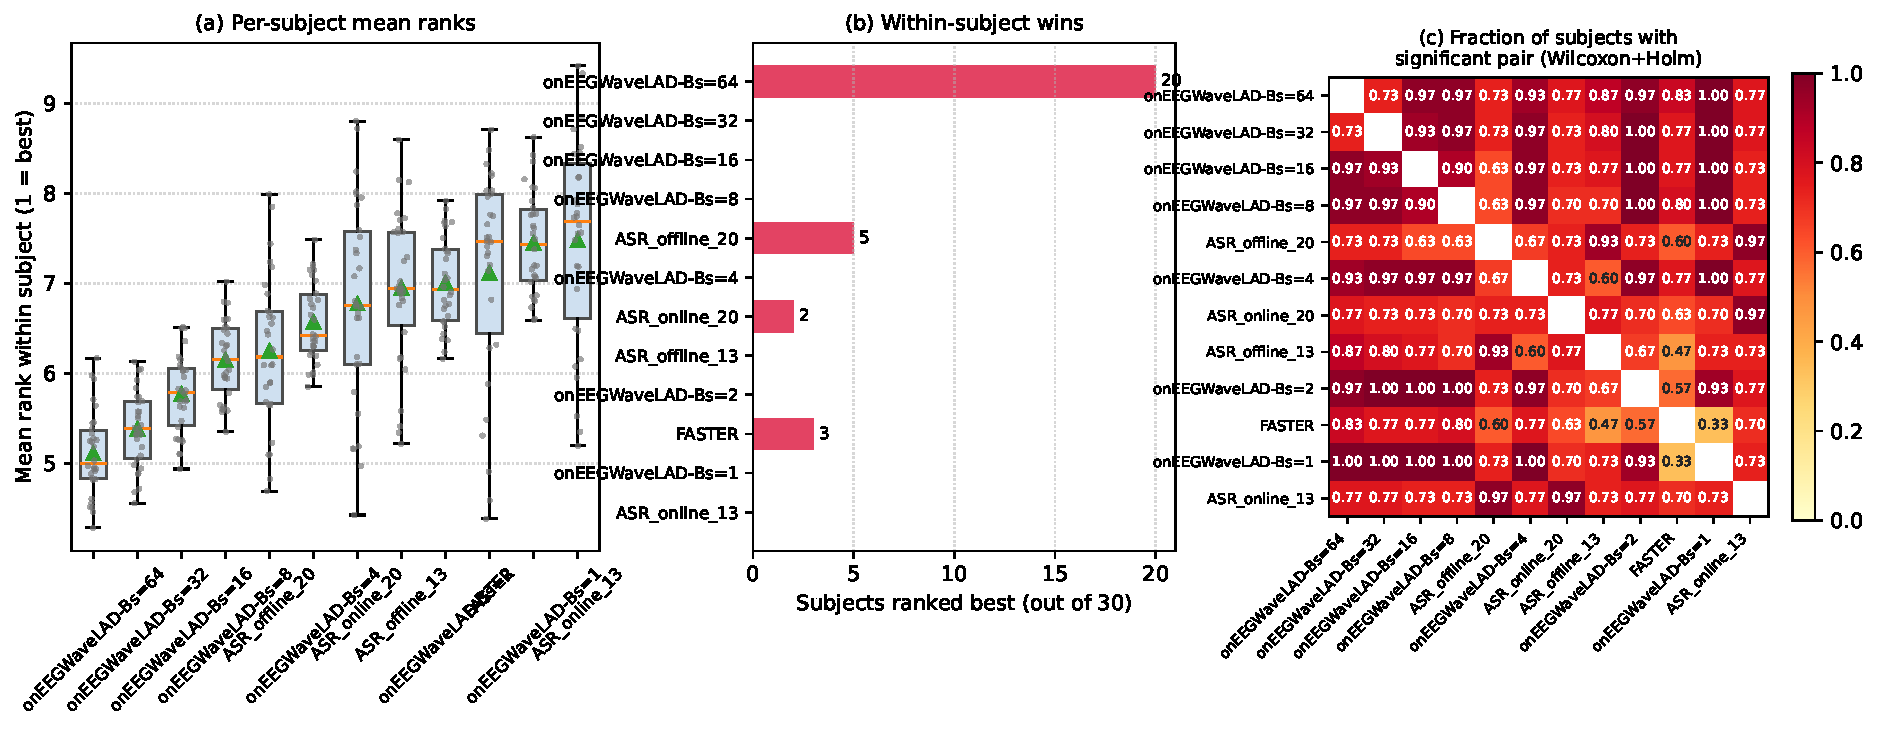
\includegraphics[width=0.95\textwidth]{Figures/CD_baseline_metric-aggregated_summary.pdf}
    \vspace{0.5em}\hrule
    \caption{Within-subject analysis: (a) Per-subject mean ranks across the twelve methods, averaged over thirty channels within each subject; (b) Win matrix showing how many times each method ranks first within a subject; (c) Pairwise significance matrix from Wilcoxon signed-rank tests with Holm correction, displaying the fraction of subjects (out of thirty) in which each pairwise comparison reaches $\alpha = 0.05$ significance. Darker cells indicate more consistent pairwise separations across the cohort. The deepest buffers separate from the shallowest in nearly all subjects; comparisons involving the baselines are less consistent, with ASR\_offline\_20 reaching significance against the four deepest buffers in $63$--$73\%$ of subjects.}
    \label{fig:cd_baseline_panels}
    \vspace{0.5em}\hrule
\end{figure}

\begin{figure}[!htb]
\hrule\vspace{0.5em}
    \centering
    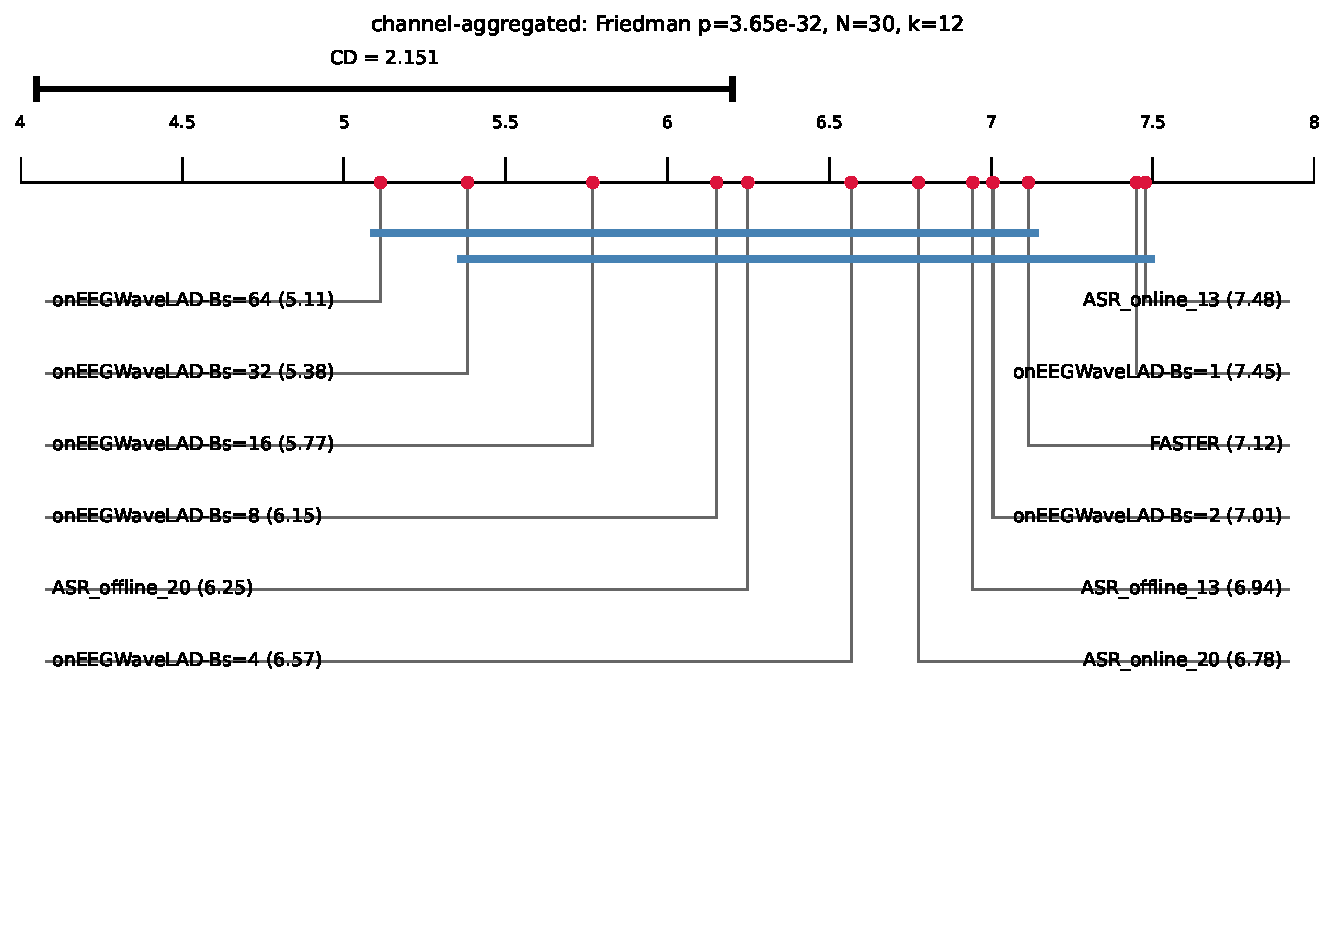
\includegraphics[width=0.9\textwidth]{Figures/CD_baseline_channel-aggregated.pdf}
    \vspace{0.5em}\hrule
    \caption{Critical difference diagram for the joint comparison of seven onEEGwaveLAD buffer configurations and five baseline methods under the channel-aggregated configuration (Friedman $p = 3.65 \times 10^{-32}$, $N = 30$ subjects, $k = 12$ methods, $\mathrm{CD} = 2.151$). Methods connected by a horizontal bar are statistically indistinguishable at $\alpha = 0.05$. The mean rank of $B_s = 8$ ($6.15$) is the shallowest buffer to exceed that of the strongest baseline, ASR\_offline\_20 ($6.25$), by a margin of $0.10$ rank units, which lies far below the critical difference and therefore denotes parity rather than superiority.}
    \label{fig:cd_baseline_aggregated}
    \vspace{0.5em}\hrule
\end{figure}

\begin{figure}[!htb]
\hrule\vspace{0.5em}
    \centering
    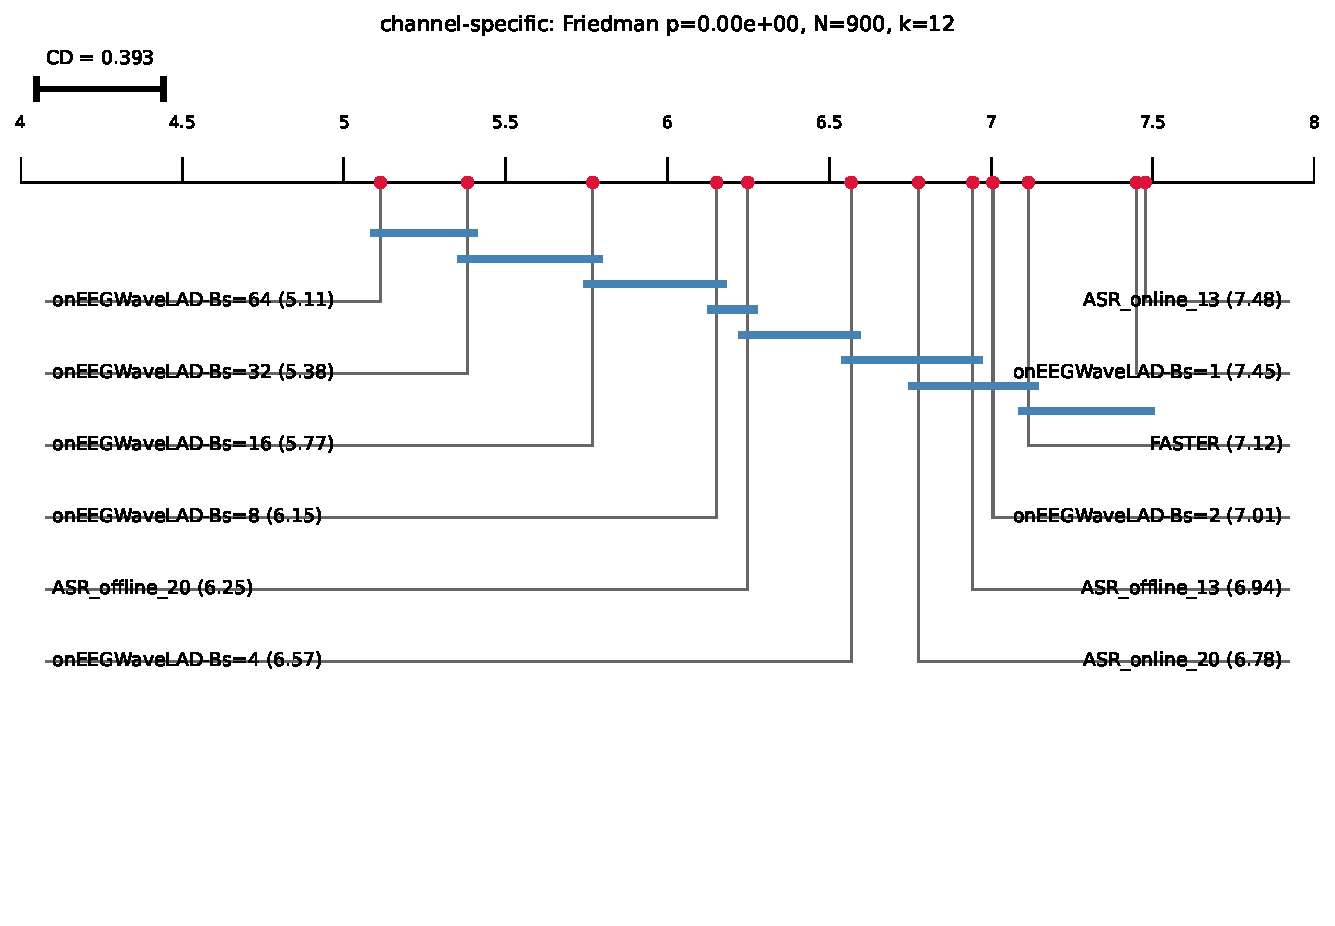
\includegraphics[width=0.9\textwidth]{Figures/CD_baseline_channel-specific.pdf}
    \vspace{0.5em}\hrule
    \caption{Critical difference diagram for the same twelve methods under the channel-specific
    configuration ($N = 900$ subject--channel pairs, $k = 12$, $\mathrm{CD} = 0.393$). The mean
    ranks are identical to those of Figure~\ref{fig:cd_baseline_aggregated}; the narrower critical
    difference follows from the larger nominal sample size obtained by pooling non-independent
    channels, and separates the deeper buffers from ASR\_offline\_20 while leaving $B_s = 8$
    indistinguishable from it. This configuration is reported as a secondary consistency check.}
    \label{fig:cd_baseline_specific}
    \vspace{0.5em}\hrule
\end{figure}


\section{Interpretation of Findings}
\label{sec:interpretation_findings}

The monotonic relation between buffer depth and aggregate denoising quality admits a straightforward mechanistic reading in terms of how the Extended Isolation Forest acquires its notion of normality. The detector partitions a population of Instantaneous Spectral Profiles and assigns anomaly scores according to how readily a profile is isolated from the rest; its capacity to distinguish a transient artefact from an unusual but legitimate fluctuation therefore depends on the volume and representativeness of the profiles held in the buffer~\parencite{hariri2019extended}. When the buffer retains only one or two profiles, the reference population is too sparse to encode the variability of nominal cortical activity, and ordinary fluctuations are isolated as readily as genuine contamination, which produces indiscriminate attenuation. As the buffer deepens, the population increasingly spans the range of states the subject occupies, the isolation boundary stabilises, and mitigation becomes selective. The diminishing returns observed beyond $B_s = 8$ follow from the same account: once the buffer holds enough profiles to characterise the subject's baseline, further history adds redundant rather than novel information, and the isolation boundary ceases to move materially.

The divergence between the two metric categories documented in
Section~\ref{subsec:impact_bs} is a direct consequence of this mechanism rather than an inconsistency in the evaluation. The similarity-oriented metrics reward the retention of the recorded waveform, so they improve as mitigation becomes more selective and the denoised signal departs less from its input. Conversely, the five artefact-removal metrics reward the enhancement of the event-locked response relative to the pre-stimulus baseline, and are consequently served by the indiscriminate attenuation that a sparse buffer produces; a detector that trims aggressively removes more contaminating energy, and is credited for doing so even where it also removes cortical signal. The two categories thus encode a genuine trade-off between preservation and suppression, and the non-monotonic trajectory of the five-metric artefact-removal category at large $B_s$ records the conservative end of that trade-off rather than any deterioration of the framework. The rebound visible when all fifteen metrics are averaged is the arithmetic consequence of combining these opposing directions, and is not interpreted as a unified physical effect.

The catastrophic negative values in $\mathrm{SNR}_{\mathrm{diff}}$ reinforce the same reading from its extreme tail. These values arise almost exclusively at $B_s \in \{1, 2\}$ and in individual channels, which is the regime in which the mechanism above predicts over-trimming: where attenuation collapses the stimulus-locked response, the ratio on which the metric rests degrades sharply, and values below $-10$~dB result in roughly $0.70$ per cent of observations. Their origin lies in the denoising behaviour itself and not in the numerical guard applied during computation. The $\pm 100$~dB cap is approached in only $0.59$ per cent of observations and reached in none, so the tail cannot be attributed to saturation of that limit. Its practical implication is confined to aggregation: a mean computed over a distribution with a tail of this length is unstable, so the median is reported alongside it and the two metric categories are examined separately.

The empirical picture obtained here is consistent with the physical expectation set out in the literature review, namely that a detector operating on a sliding history improves as that history lengthens and subsequently converges, and it does not reproduce the symmetric degradation that a concept-drift account would predict at the upper end of the range~\parencite{gama2014survey, longo2025oneegwavelad}. Across the grid examined, aggregate performance improves monotonically as far as $B_s = 64$; no buffer depth within $[1, 64]$ exhibits the deterioration that would follow from a buffer saturated with outdated states. This does not establish that such a regime cannot exist, since a buffer sufficiently long to span substantial changes in cognitive state was not tested here, and the range examined is bounded by the grid rather than by a physical argument. The conclusion supported by the data is narrower and directional: within the practical range relevant to online deployment, the operative constraint is insufficient history rather than excessive history, so the quantity of interest is a lower bound.

Two aspects of the analysis require explicit methodological comment, since both affect how the reported threshold should be read. The elbow located by the Kneedle procedure moved from $B_s = 4$ in the coarse stage to $B_s = 8$ in the refined stage, and this shift is attributable in part to the denser sampling of the interval and in part to the change of horizontal scale from logarithmic to linear, to which curvature-based elbow detection is sensitive~\parencite{satopaa2011finding}. Neither stage is discarded. The refined stage is preferred because it samples the region of interest more densely and preserves the absolute spacing of the buffer values, and the coarse stage is retained as the analysis that identified where to refine. Furthermore, the parity between $B_s = 8$ and the strongest baseline is established at the subject level, where the critical difference is wide; the deeper buffers rank ahead of every baseline without reaching that threshold. The framework is therefore best characterised as matching established automated methods once the buffer is sufficiently deep, rather than as displacing them.

\section{Effectiveness and Shortcomings of Findings}
\label{sec:effectiveness_shortcomings}

The findings documented in the preceding sections establish a convergence lower bound and situate it relative to baseline methods, but their practical utility depends on how robustly they generalise across subjects and analytical choices, and on how honestly their limitations are acknowledged. This section first assesses the stability of the threshold across the thirty-subject cohort and the three statistical configurations, then documents the unresolved methodological gaps that delimit the scope of the conclusions and remain the principal open questions for future work.

    \subsection{Generalisability and Robustness Across Subjects}
    \label{subsec:generalisability}

The threshold reported in Section~\ref{subsec:identification_threshold} rests on the full thirty-subject N170 cohort evaluated across thirty channels, so that the behaviour described reflects inter-subject variability rather than a single favourable recording. Its stability was examined along three axes. Across analytical configurations, the monotonic ordering of buffer sizes is reproduced under channel-aggregated, channel-specific and within-subject analyses, which differ in their unit of replication and consequently in their critical differences but not in their point estimates or in the direction of the effect. Across the two grid stages, the coarse and refined searches locate the onset of diminishing returns in the same region, and the median-aggregated trajectories of both stages converge on $B_s \approx 8$. Across individual recordings, the within-subject Friedman tests reject the null hypothesis in all thirty subjects, and the contrasts between the deeper and the shallowest buffers recur in at least twenty-nine of thirty. The convergence behaviour on which the lower bound rests is therefore not an artefact of pooling.

Two qualifications bound this generalisability. The consistency established above concerns the \emph{ordering} of buffer sizes and the \emph{location} of the convergence region; it does not extend to the parity claim against the baselines, which is supported at the subject level by a rank difference of $0.10$ and is reproduced at the individual level in only $63$ to $73$ per cent of subjects. Moreover, the entire analysis is conducted within a single paradigm and cohort, on stimulus-locked recordings from a thirty-channel laboratory montage, and the recommended lower bound should be read as specific to that setting rather than as a device-independent constant. 

    \subsection{Unresolved Knowledge Gaps for Future Extensions}
    \label{subsec:unresolved_gaps}

Several limitations delimit the scope of the conclusions and indicate where further work is required. The wavelet decomposition passes the terminal approximation coefficients through unmodified, so spectral content below approximately $2$~Hz is not subject to mitigation; the detail band covering roughly $2$ to $4$~Hz, which carries the greater part of blink energy, is processed, and the residual gap is therefore confined to the $[0, 2]$~Hz range rather than encompassing the whole of the delta band. Consequently, very slow drift is attenuated only by the $1$~Hz high-pass applied during preprocessing and not by the framework itself. The expansion step was held at $E_s = 35$ throughout, so no interaction between the mitigation footprint and the buffer depth was examined, and the reported bound is conditional on that setting. A grid over $E_s$ jointly with $B_s$ remains open as future work.


The evaluation protocol imposes a further constraint that shapes how the metric trajectories should be understood. Real recordings supply no artefact-free reference, so the similarity-oriented metrics are computed against the contaminated input and in effect quantify how much the signal was altered; they consequently favour conservative mitigation on structural grounds, independently of whether the material removed was cortical or artefactual. Ranking across a heterogeneous suite and benchmarking against independent baselines mitigate but do not eliminate this bias, and a validation on data with a known clean reference -- obtained by means other than injecting synthetic artefacts into already contaminated recordings, which was judged indefensible for this dataset -- would be required to resolve it. Per-window processing time was not recorded during the batch evaluation, so the real-time viability of the identified lower bound cannot be verified from these experiments; online deployment testing with latency profiling remains necessary to confirm that $B_s = 8$ sustains
throughput without accumulating delay.

Two further qualifications concern the strength of the central claims. The parity between $B_s = 8$ and ASR\_offline\_20 rests on a rank separation of $0.10$ against a critical difference of $2.151$; the deeper buffers rank ahead of all baselines but likewise without reaching that threshold, so no buffer configuration is established as significantly superior to the baseline family at the subject level, and the separation observed under the pooled channel-specific analysis should not be read as strengthening that claim. The median aggregation, finally, is a robustness check rather than an independent third confirmation: because ten of the fifteen metrics belong to the similarity-oriented category, the median tracks that majority and suppresses the five artefact-removal metrics by construction, so it re-expresses the convergence of the similarity family under a robust aggregator instead of synthesising all fifteen on equal terms. Establishing an adaptive threshold in place of the fixed $T_a = 0.55$, and characterising whether a sufficiently long buffer eventually induces the drift regime that the present range does not exhibit, remain the principal open questions for future work.
\chapter{Conclusion}
\label{chap:conclusion}

\section{Research Summary and Experimental Findings}
\label{sec:research_summary}

This thesis quantified the convergence lower bound for the onEEGwaveLAD framework's Adaptive Buffer Size parameter ($B_s$), a hyperparameter that controls how much historical context the Extended Isolation Forest uses to distinguish transient artefacts from neural signals~\parencite{longo2025oneegwavelad}. The lower bound, denoted $X$ and defined as the smallest buffer size beyond which evaluation metrics cease to improve meaningfully, was not established before this work.

A two-stage grid search (Stage 1: exponential spacing across $B_s \in \{1,2,4,8,16,32,64\}$; Stage 2: linear refinement across $B_s \in \{4,6,8,10,12,14,16,18\}$) was conducted on the full thirty-subject ERP-CORE N170 cohort, with performance assessed across fifteen metrics spanning time-domain, frequency-domain, and statistical measures~\parencite{kappenman2021erp, satopaa2011finding}. Seven buffer configurations and five baseline methods (FASTER-ICA and four ASR variants) were ranked together using non-parametric statistical testing~\parencite{nolan2010faster, mullen2015real, friedman1937use}.

The empirical findings show the convergence lower bound at approximately $B_s = 8$, supported by two independent lines of evidence. First, Kneedle elbow detection applied to normalised marginal improvement curves identified the onset of diminishing returns at $B_s = 4$ (Stage 1) and $B_s = 8$ (Stage 2)~\parencite{satopaa2011finding}. Second, rank-based comparison showed that $B_s = 8$ is the smallest buffer reaching parity with the strongest baseline (ASR\_offline\_20, rank separation $\Delta = 0.10 < \mathrm{CD} = 2.151$). Buffers smaller than eight are outranked by at least one baseline, whereas buffers of eight and larger enter a regime of diminishing returns.

The fifteen-metric suite exhibited directional heterogeneity. Ten similarity-oriented metrics (correlation, mutual information, RMSE, band power preservation, and MSC in alpha/beta bands) favoured larger buffers and improved monotonically. Five artefact-removal metrics (SNR-Diff, PSNR-Diff, and MSC in theta/gamma/delta bands) favoured smaller buffers and showed non-monotonic behaviour at large $B_s$. The rebound observed when averaging these oppositely directed metrics is a mathematical artefact of aggregation, not a physical degradation mechanism, and shows the necessity of stratified analysis~\parencite{longo2025oneegwavelad}. Friedman tests across three statistical configurations confirmed that buffer size has a significant, monotonic effect on performance.

\section{Summary of Core Contributions}
\label{sec:core_contributions}
Four contributions emerge from this work. First, it quantifies the convergence lower bound ($B_s \approx 8$) for the onEEGwaveLAD framework through a full-cohort evaluation across thirty subjects, thirty channels, and fifteen heterogeneous metrics. The two-stage grid search strategy provides a methodologically sound approach when the target quantity is a lower bound rather than an optimum. Second, the multi-criteria convergence protocol combines absolute improvement thresholds, noise floor estimation, and Kneedle elbow detection on raw metric trajectories~\parencite{satopaa2011finding}. Rank-based procedures can obscure when underlying metric values level off; this approach overcomes that limitation, and the stratified treatment of similarity-oriented versus artefact-removal metric families shows how to handle heterogeneous evaluation suites. Third, the convergence lower bound is compared to established multi-channel baselines: $B_s = 8$ is the smallest buffer at which onEEGwaveLAD reaches parity with these methods~\parencite{nolan2010faster, mullen2015real}. This shows that a single-channel, reference-free framework can match spatial decomposition methods with a properly configured buffer. Fourth, two implementation-level phenomena are explained: the non-monotonic behaviour of artefact-removal metrics comes from their directional bias rather than numerical saturation, and the median aggregation tracks the similarity-metric majority rather than combining all metrics equally. These explanations confirm the reported threshold rests on sound interpretation.

\section{Implications and Future Work}
\label{sec:implications_future}

The convergence lower bound has direct consequences for practitioners deploying the framework and for researchers extending this investigation. The practical implications for real-world BCI applications and for evaluating adaptive systems are examined first, followed by directions for future work that would test the generalisability of the present findings and address their limitations.

\subsection{Practical Implications}

For practitioners deploying the onEEGwaveLAD framework under conditions similar to those examined here, the recommendation is to adopt a minimum buffer size of eight or larger. Buffers below this threshold remain outranked by multi-channel baselines, whereas buffers substantially larger than eight yield diminishing marginal gains. This recommendation assumes a fixed expansion step $E_s = 35$; joint optimisation over both parameters remains future work~\parencite{longo2025oneegwavelad}. The finding that onEEGwaveLAD at $B_s = 8$ reaches parity with the strongest baseline supports its use in single-channel, real-time applications where multi-channel spatial decomposition methods are impractical~\parencite{makeig1996independent, mullen2015real}. This validation comes from a full-cohort evaluation on naturalistic ERP recordings, so the reported behaviour reflects robustness across heterogeneous contamination regimes~\parencite{kappenman2021erp}. Methodologically, the divergence between similarity-oriented and artefact-removal metric families shows the necessity of stratified analysis when evaluation suites are heterogeneous. The protocol developed here--combining convergence criteria on raw trajectories with rank-based testing and stratified robustness checks--applies generally to hyperparameter optimisation where quality is multi-dimensional~\parencite{friedman1937use}.

\subsection{Future Extensions}

Several extensions would strengthen the empirical foundation. Joint optimisation of buffer size ($B_s$) and expansion step ($E_s$) would show how the mitigation footprint interacts with buffer depth. Testing on other paradigms (resting-state, motor-imagery BCI, vigilance monitoring) would show whether $B_s \approx 8$ generalises beyond stimulus-locked protocols~\parencite{kappenman2021erp}. Testing buffers larger than sixty-four on long recordings would show whether performance eventually declines when the buffer spans substantial changes in cognitive state~\parencite{gama2014survey}. Implementing an adaptive anomaly threshold $T_a$ that adjusts per subject or per channel, rather than the global constant $0.55$ used here, could improve sensitivity. Deployment profiling on representative edge hardware would verify that $B_s = 8$ sustains real-time throughput without accumulating latency. Extending anomaly detection to the approximation coefficients would address contamination below 2 Hz, though the bulk of ocular artefact energy resides in the processed 2-4 Hz detail band~\parencite{longo2025oneegwavelad}. These extensions would test the generalisability of the convergence lower bound and identify boundary conditions under which the framework's behaviour changes. The methodological framework developed here provides a template for such investigations.

\backmatter

\printbibliography

\appendix

\chapter{Supplementary Visualisations}
\label{app:supplementary_vis}

This appendix provides additional visualisations that complement the main text, including the animated buffer evolution sequence and the complete collection of critical difference diagrams for all configurations and individual metrics.

\section{Animated Buffer Evolution}
\label{app:animated_buffer}

The temporal evolution of the sliding buffer mechanism, introduced in Section~\ref{subsec:qualitative_visualization} as Visualisation 2, is presented as an animated sequence showing how the population of Instantaneous Spectral Profiles changes as successive windows are ingested. The animation spans a continuous segment of the recording (subject 19, channel Fp1, $B_s = 8$) and illustrates how contaminated profiles enter the buffer, persist for $B_s$ steps, and then slide out as newer data arrives.

The animated sequence is available at the following permanent repository:

\href{https://github.com/Areca293/Evaluating-the-Isolation-Forest-unsupervised-anomaly-detector-of-onEEGWaveLAD/blob/main/vis2\_buffer\_evolution.gif}{GitHub: Areca293/onEEGwaveLAD (vis2\_buffer\_evolution.gif)}

Each frame corresponds to one window in the continuous recording. The vertical axis displays the $B_s$ most recent ISPs retained in the buffer (rows represent historical samples, with the current window at the top and older profiles below), and the horizontal axis spans the scaleogram feature dimensions. Heatmap intensity encodes normalised feature amplitude (magma colourmap: dark = low, bright = high). Clean epochs yield relatively uniform low-intensity patterns, while contaminated epochs introduce bright high-amplitude bands. This temporal visualisation demonstrates how a sufficiently deep buffer ($B_s \geq 8$) retains enough history to distinguish transient artefacts from legitimate neural variability.

\section{Complete Critical Difference Diagrams}
\label{app:complete_cd}

This section presents the complete collection of critical difference (CD) diagrams for all statistical configurations and individual metrics. The main text (Chapter~\ref{chap:results}) presents representative CD diagrams; here we provide the full set for transparency and reproducibility.

The diagrams are organised into three groups: (1) seven-buffer configuration comparisons, which examine the monotonic effect of buffer size within the onEEGwaveLAD framework; (2) twelve-method comparisons, which situate the buffer configurations against five baseline methods to establish competitive parity; and (3) single-metric diagrams, which reveal the directional preferences of each evaluation metric and corroborate the classification into similarity-oriented (10 metrics) and artefact-removal (5 metrics) categories.

For the seven-buffer and twelve-method comparisons, multiple visualization formats are provided: channel-aggregated and channel-specific configurations establish statistical significance under different assumptions about within-subject dependence, while metric-aggregated panels, pooled views, and summary statistics illustrate the consistency of the buffer size effect across individual subjects.

For the single-metric diagrams, two complementary views are provided for each of the fifteen metrics: seven-buffer comparison (showing monotonic or non-monotonic behaviour across $B_s \in \{1, 2, 4, 8, 16, 32, 64\}$) and twelve-method comparison (situating buffer configurations against baseline methods). All single-metric diagrams use the channel-aggregated configuration ($N = 30$ subjects) from Stage 1 coarse grid.

\begin{figure}[!htb]
\hrule
\vspace{0.5em}
\centering
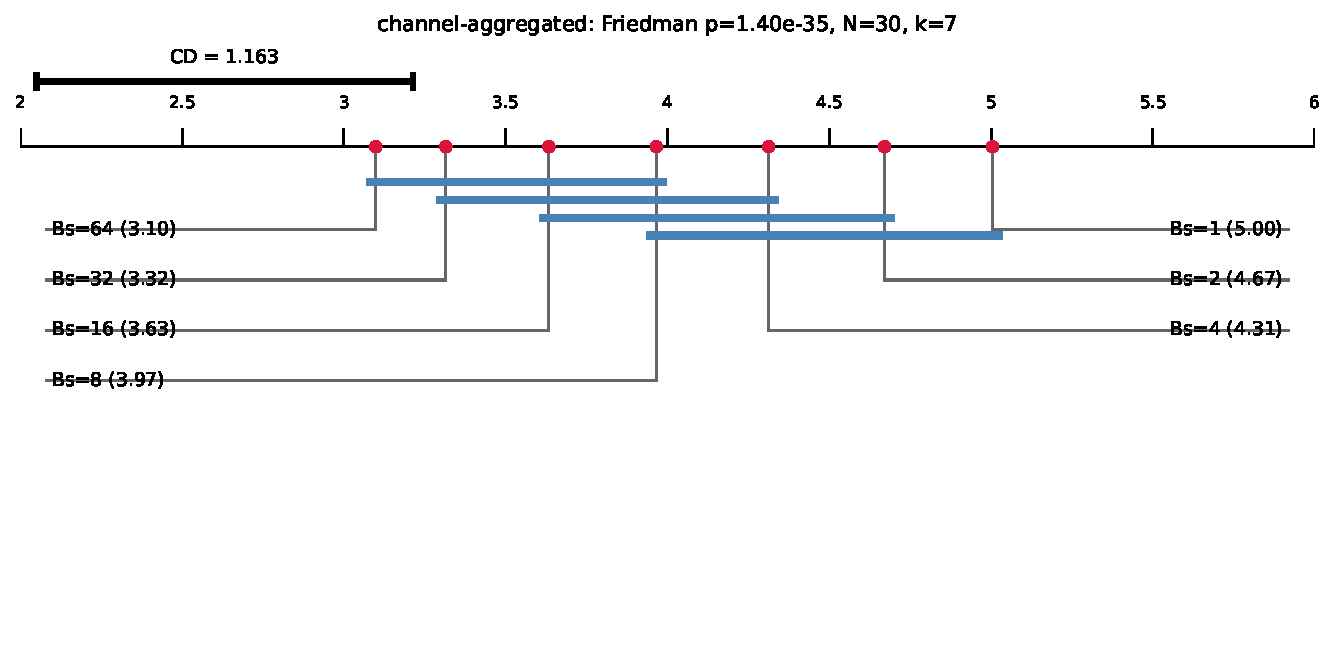
\includegraphics[width=0.85\textwidth]{Figures/CD_Bs_channel-aggregated.pdf}
\vspace{0.5em}
\hrule
\caption{Seven-buffer comparison, channel-aggregated configuration (Friedman $p = 1.40 \times 10^{-35}$, $N = 30$ subjects, $k = 7$ methods, $\mathrm{CD} = 1.163$). $B_s = 8$ is the smallest buffer lying within the critical difference interval of $B_s = 64$.}
\label{fig:cd_bs_aggregated}
\vspace{0.5em}
\hrule
\end{figure}

\begin{figure}[!htb]
\hrule
\vspace{0.5em}
\centering
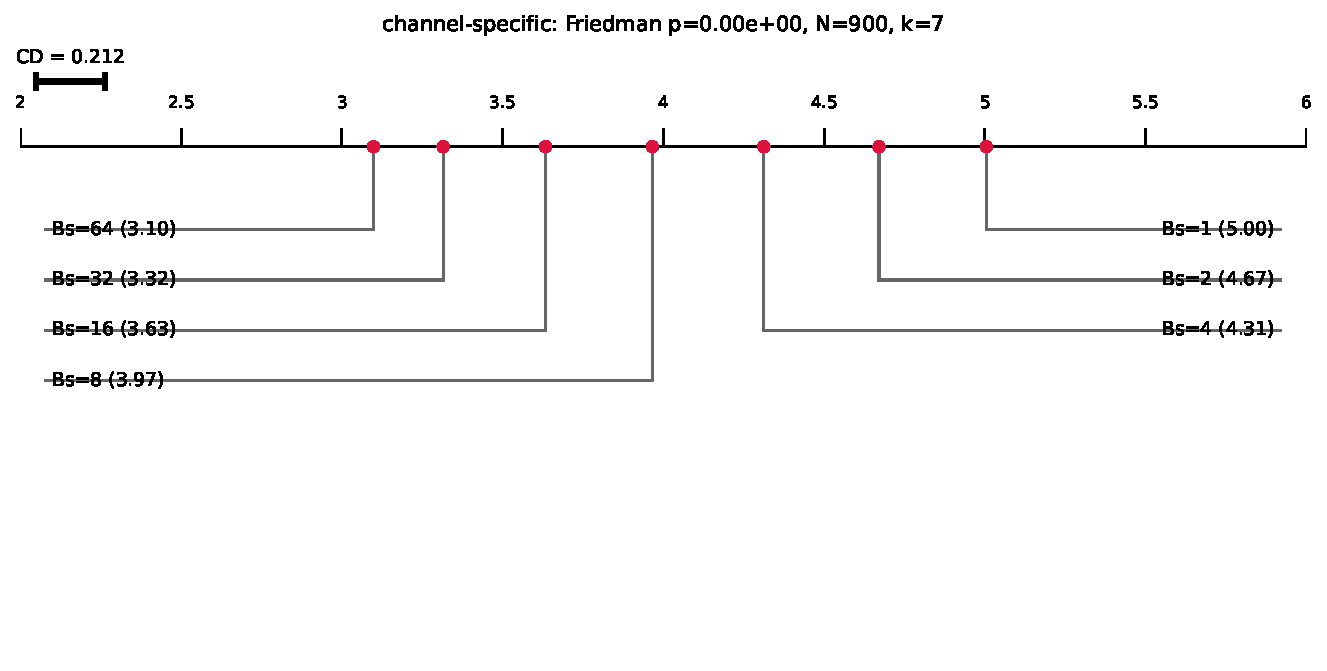
\includegraphics[width=0.85\textwidth]{Figures/CD_Bs_channel-specific.pdf}
\vspace{0.5em}
\hrule
\caption{Seven-buffer comparison, channel-specific configuration (Friedman $p < 10^{-300}$, $N = 900$ subject-channel pairs, $k = 7$ methods, $\mathrm{CD} = 0.212$).}
\label{fig:cd_bs_specific}
\vspace{0.5em}
\hrule
\end{figure}

\begin{figure}[!htb]
\hrule
\vspace{0.5em}
\centering
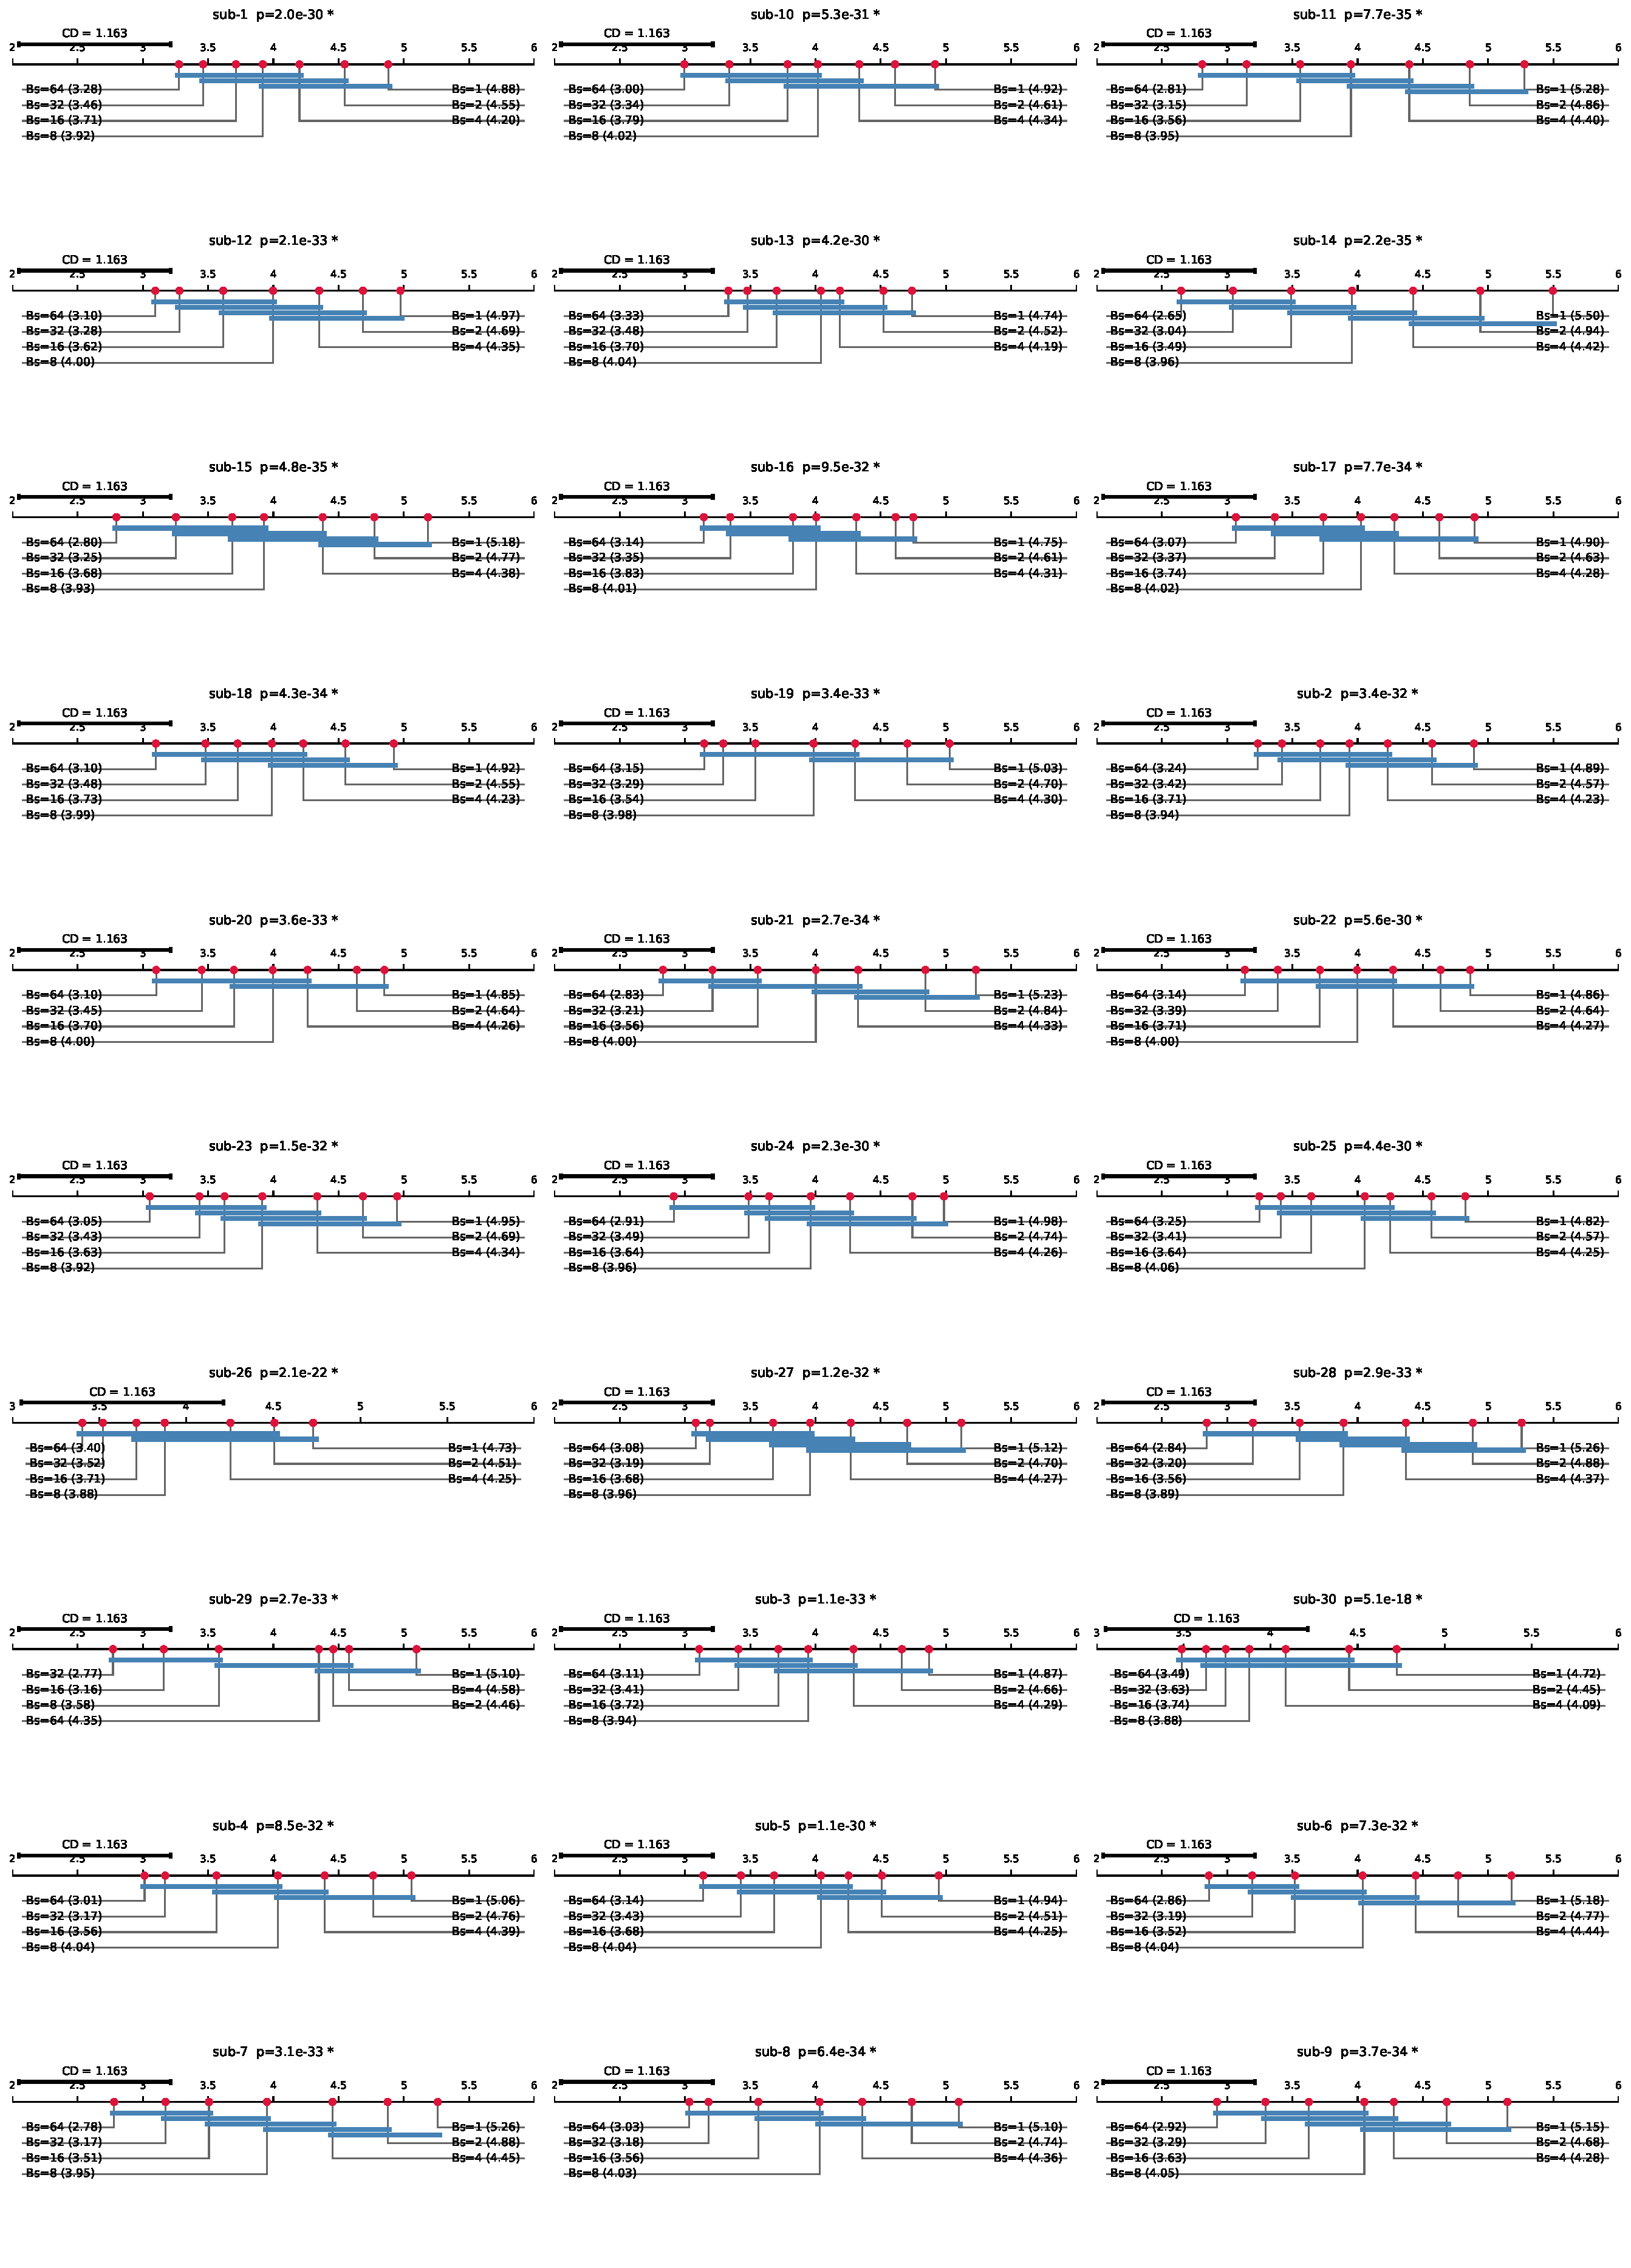
\includegraphics[width=\textwidth]{Figures/CD_Bs_metric-aggregated_panels.pdf}
\vspace{0.5em}
\hrule
\caption{Seven-buffer comparison, metric-aggregated panels across all thirty subjects. Each panel shows one subject's ranking. The monotonic ordering is consistent across subjects.}
\label{fig:cd_bs_panels}
\vspace{0.5em}
\hrule
\end{figure}

\begin{figure}[!htb]
\hrule
\vspace{0.5em}
\centering
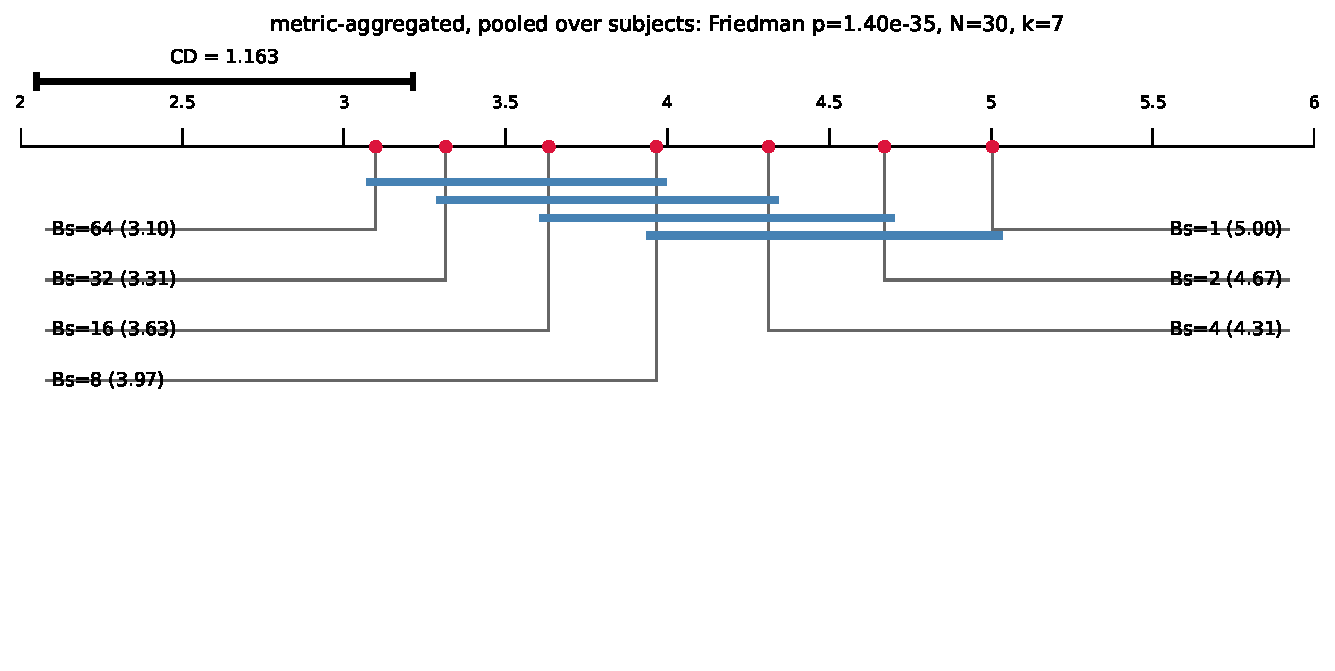
\includegraphics[width=0.85\textwidth]{Figures/CD_Bs_metric-aggregated_pooled.pdf}
\vspace{0.5em}
\hrule
\caption{Seven-buffer comparison, metric-aggregated pooled view.}
\label{fig:cd_bs_pooled}
\vspace{0.5em}
\hrule
\end{figure}

\begin{figure}[!htb]
\hrule
\vspace{0.5em}
\centering
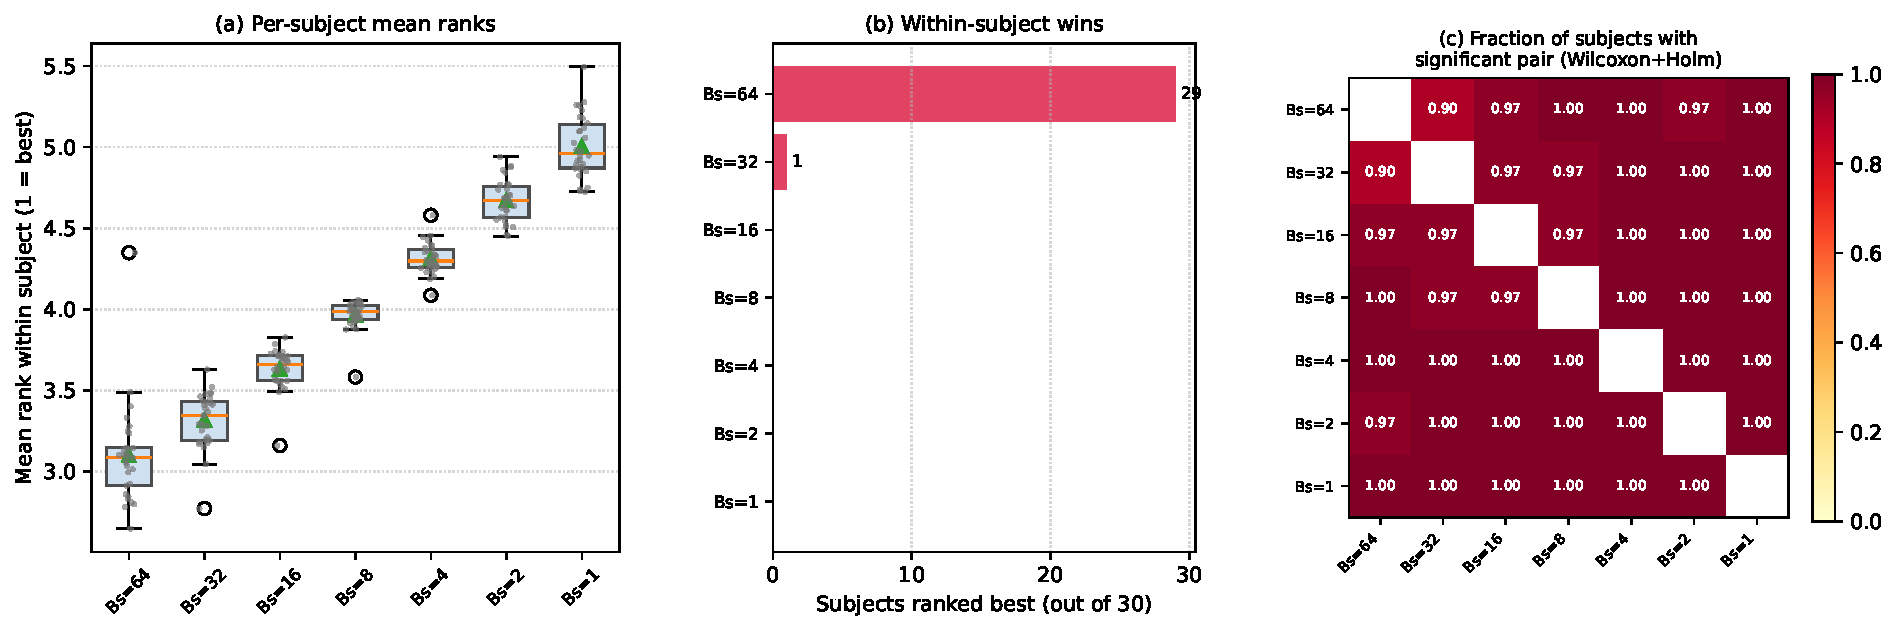
\includegraphics[width=\textwidth]{Figures/CD_Bs_metric-aggregated_summary.pdf}
\vspace{0.5em}
\hrule
\caption{Seven-buffer comparison, summary statistics: (a) boxplot of ranks; (b) mean rank trajectory; (c) pairwise critical difference matrix.}
\label{fig:cd_bs_summary}
\vspace{0.5em}
\hrule
\end{figure}

\begin{figure}[!htb]
\hrule
\vspace{0.5em}
\centering
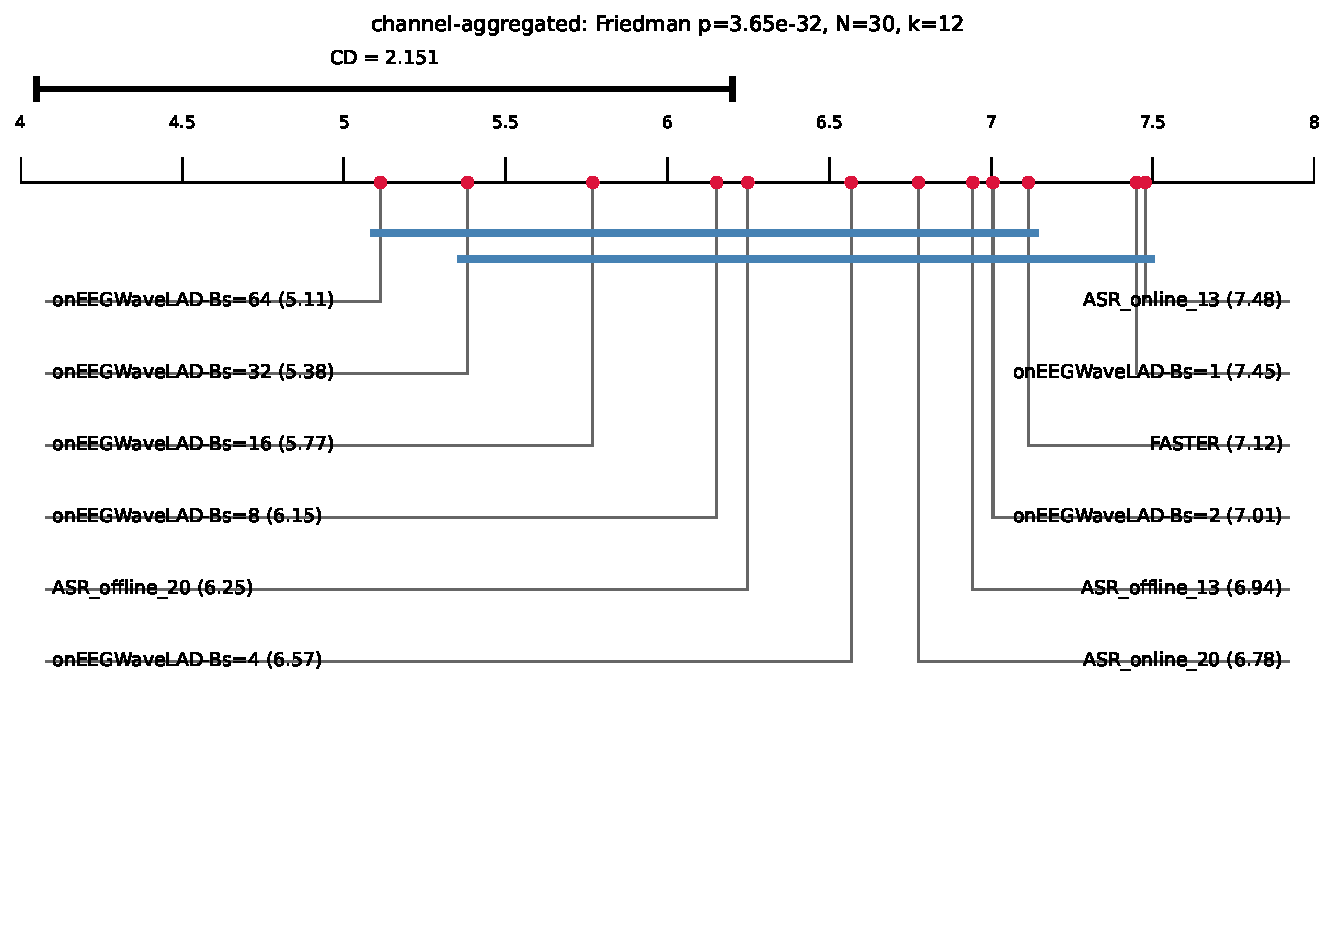
\includegraphics[width=0.95\textwidth]{Figures/CD_baseline_channel-aggregated.pdf}
\vspace{0.5em}
\hrule
\caption{Twelve-method comparison, channel-aggregated configuration (Friedman $p = 3.65 \times 10^{-32}$, $N = 30$ subjects, $k = 12$ methods, $\mathrm{CD} = 2.151$). $B_s = 8$ is the smallest buffer surpassing every baseline, with parity to ASR\_offline\_20 ($\Delta = 0.10 < \mathrm{CD}$).}
\label{fig:cd_baseline_aggregated_appendix}
\vspace{0.5em}
\hrule
\end{figure}

\begin{figure}[!htb]
\hrule
\vspace{0.5em}
\centering
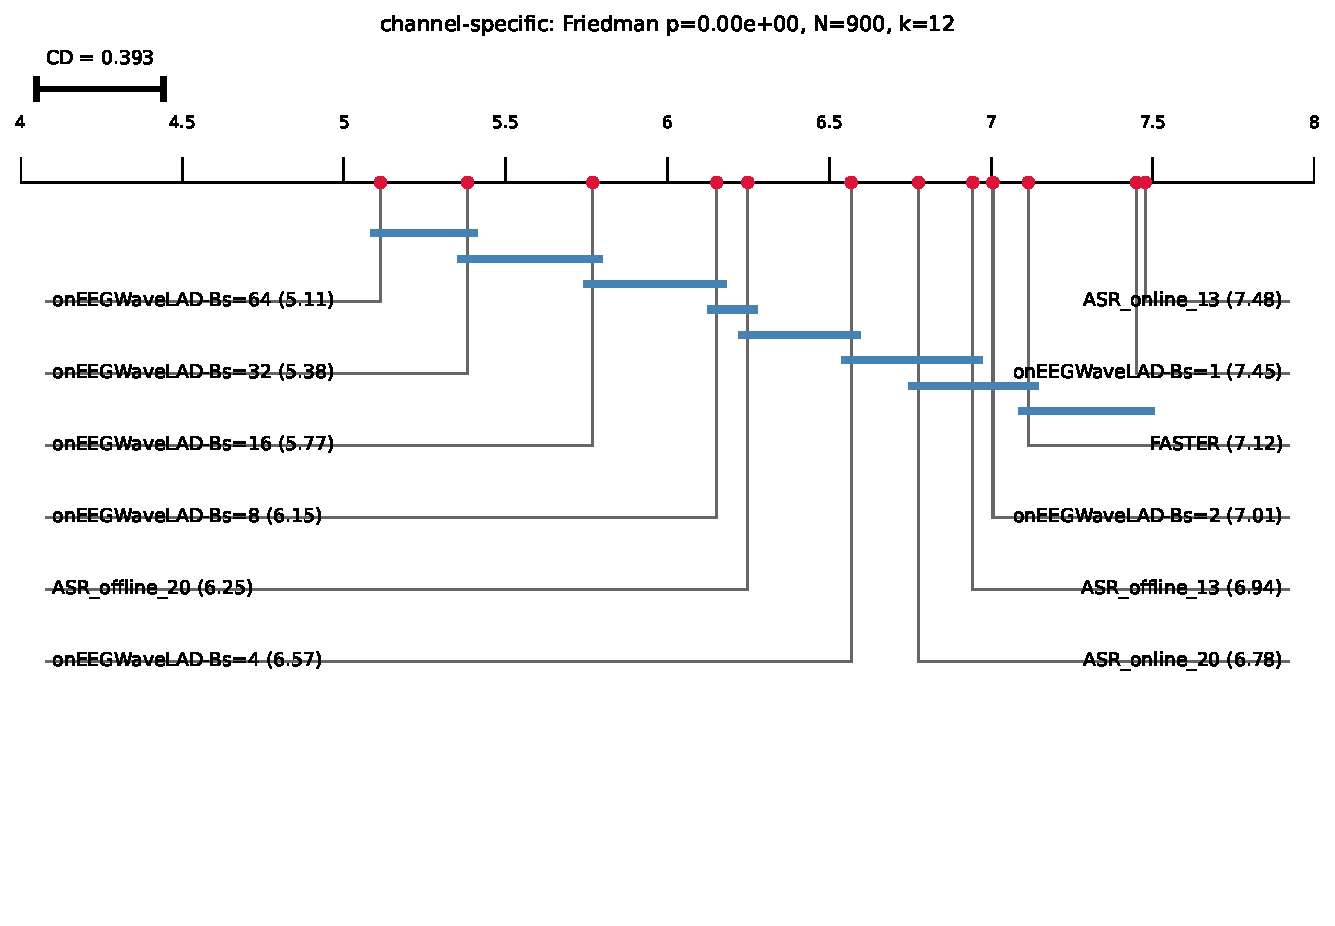
\includegraphics[width=0.95\textwidth]{Figures/CD_baseline_channel-specific.pdf}
\vspace{0.5em}
\hrule
\caption{Twelve-method comparison, channel-specific configuration (Friedman $p < 10^{-300}$, $N = 900$ subject-channel pairs, $k = 12$ methods, $\mathrm{CD} = 0.393$).}
\label{fig:cd_baseline_specific_appendix}
\vspace{0.5em}
\hrule
\end{figure}

\begin{figure}[!htb]
\hrule
\vspace{0.5em}
\centering
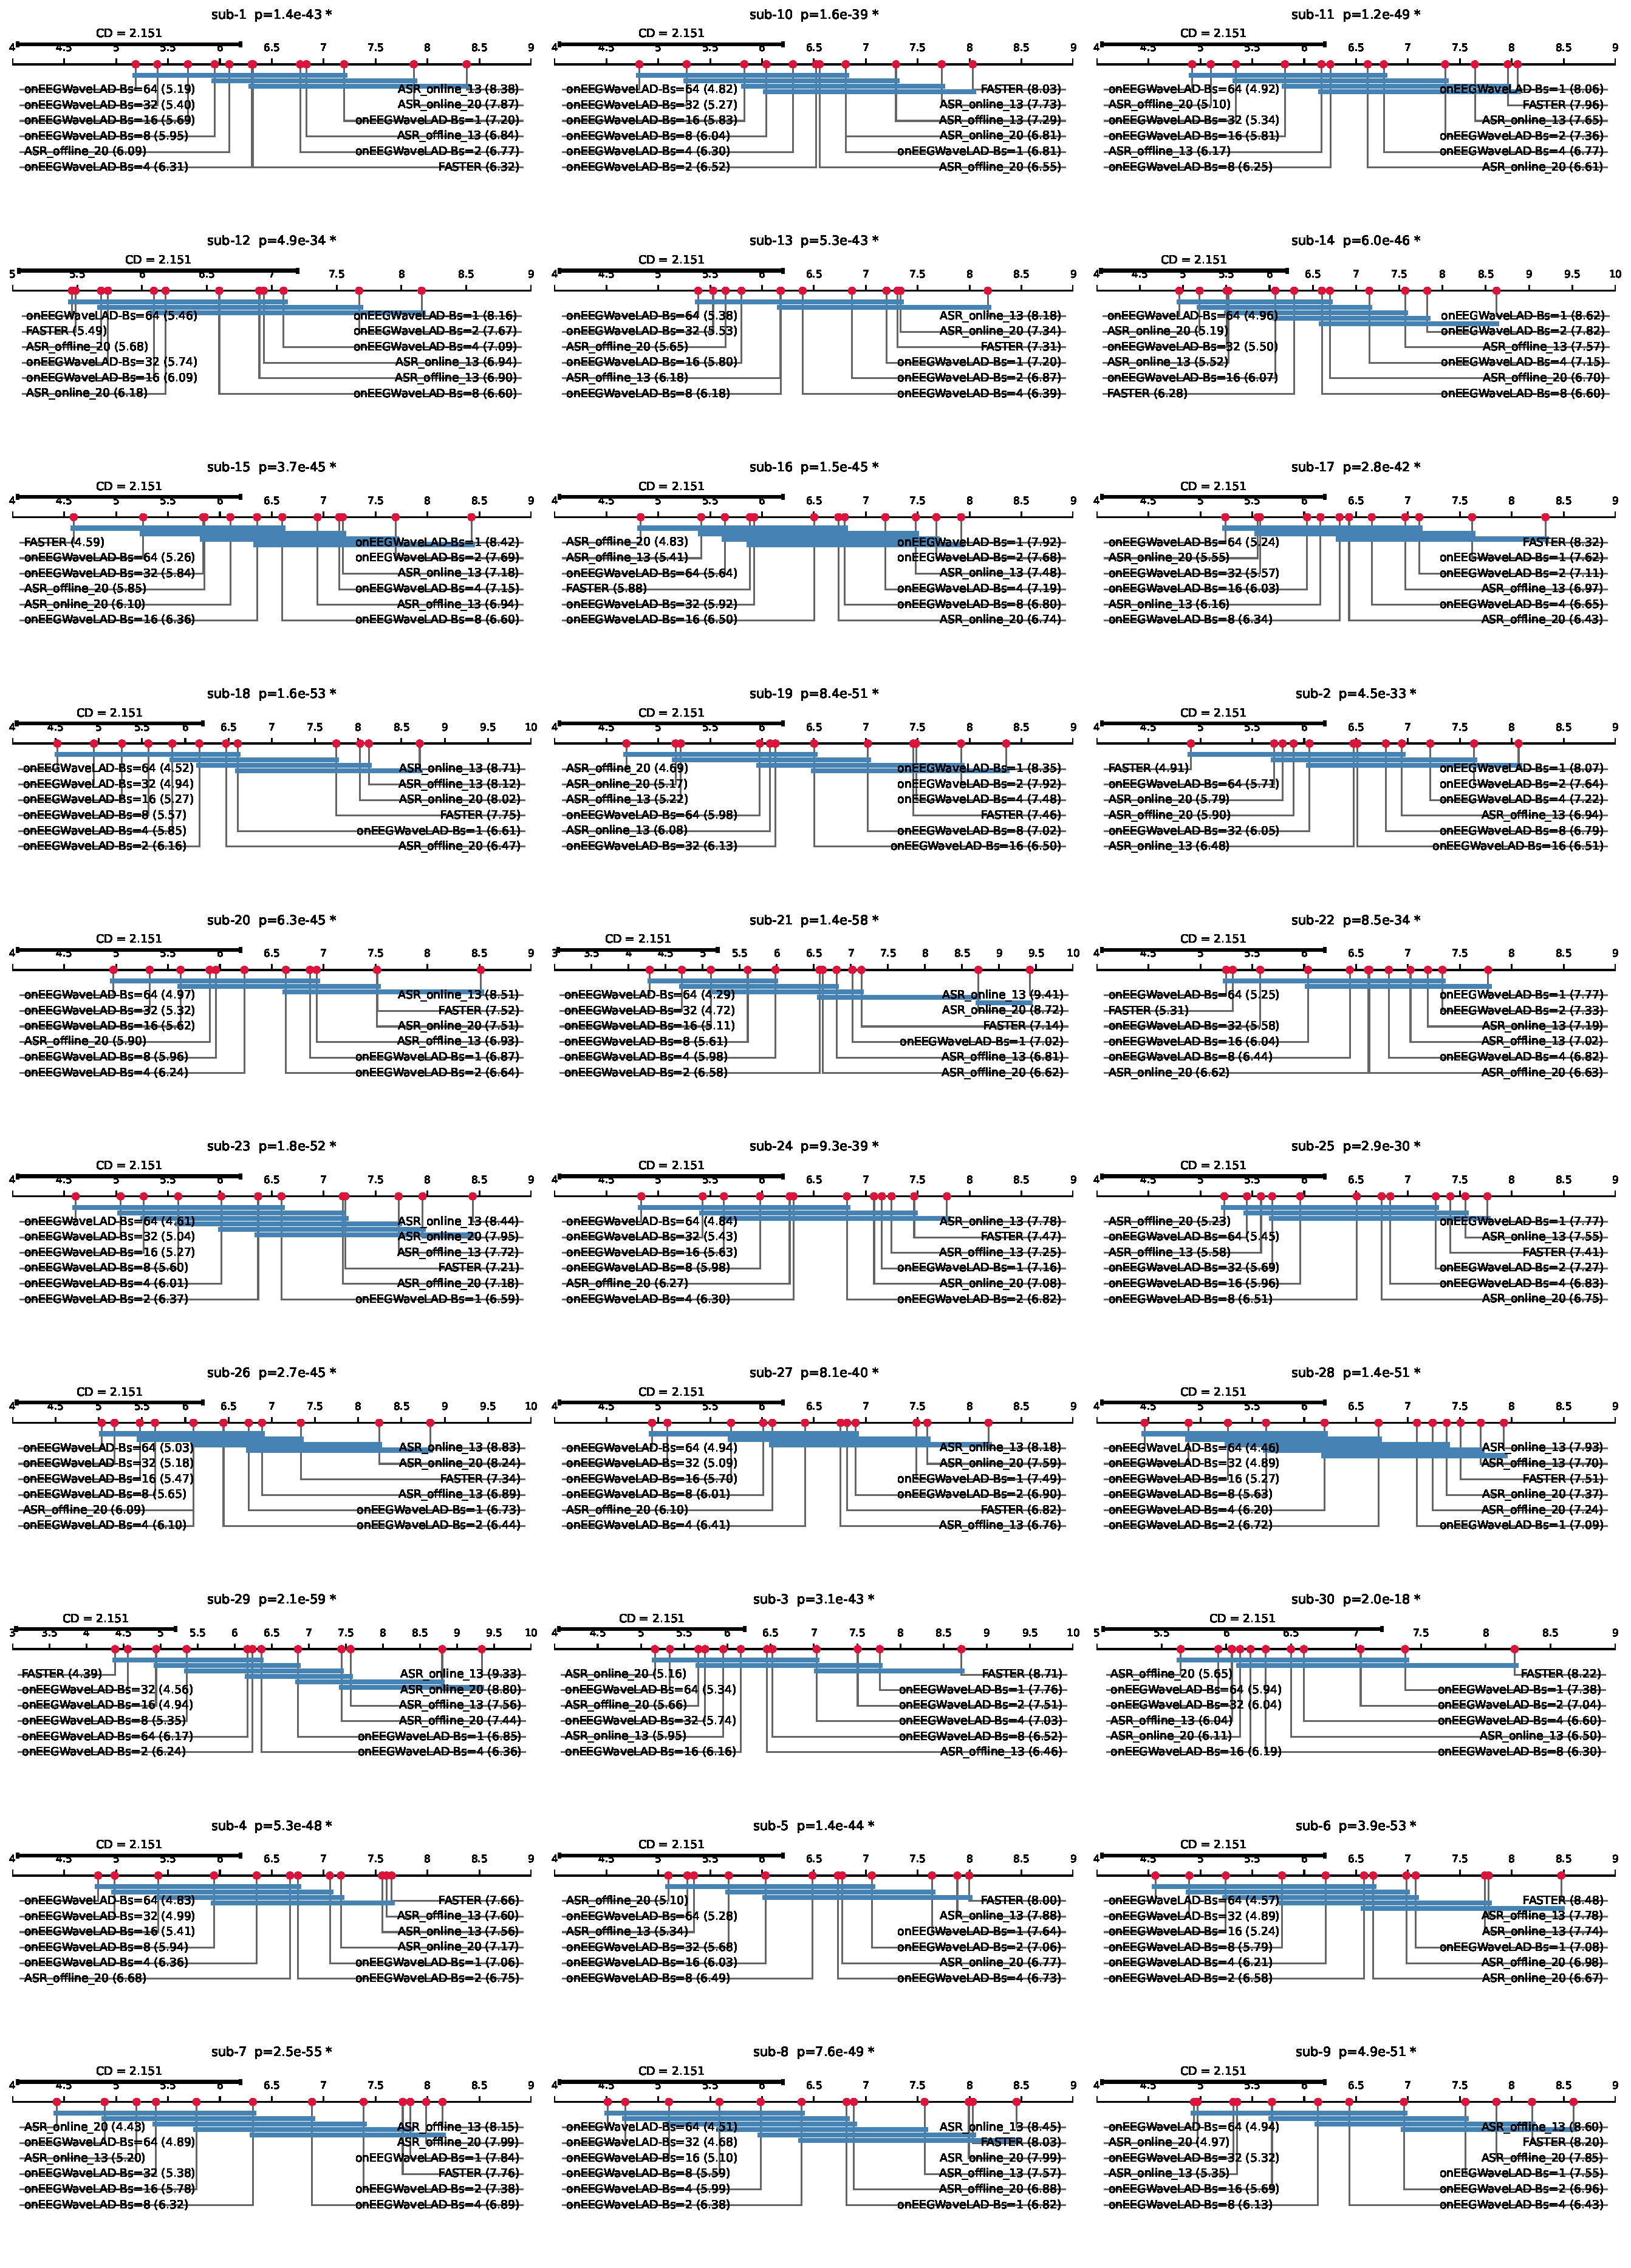
\includegraphics[width=\textwidth]{Figures/CD_baseline_metric-aggregated_panels.pdf}
\vspace{0.5em}
\hrule
\caption{Twelve-method comparison, metric-aggregated panels across all thirty subjects. The consistent ordering demonstrates that the convergence lower bound at $B_s = 8$ is robust at the individual level.}
\label{fig:cd_baseline_panels_appendix}
\vspace{0.5em}
\hrule
\end{figure}

\begin{figure}[!htb]
\hrule
\vspace{0.5em}
\centering
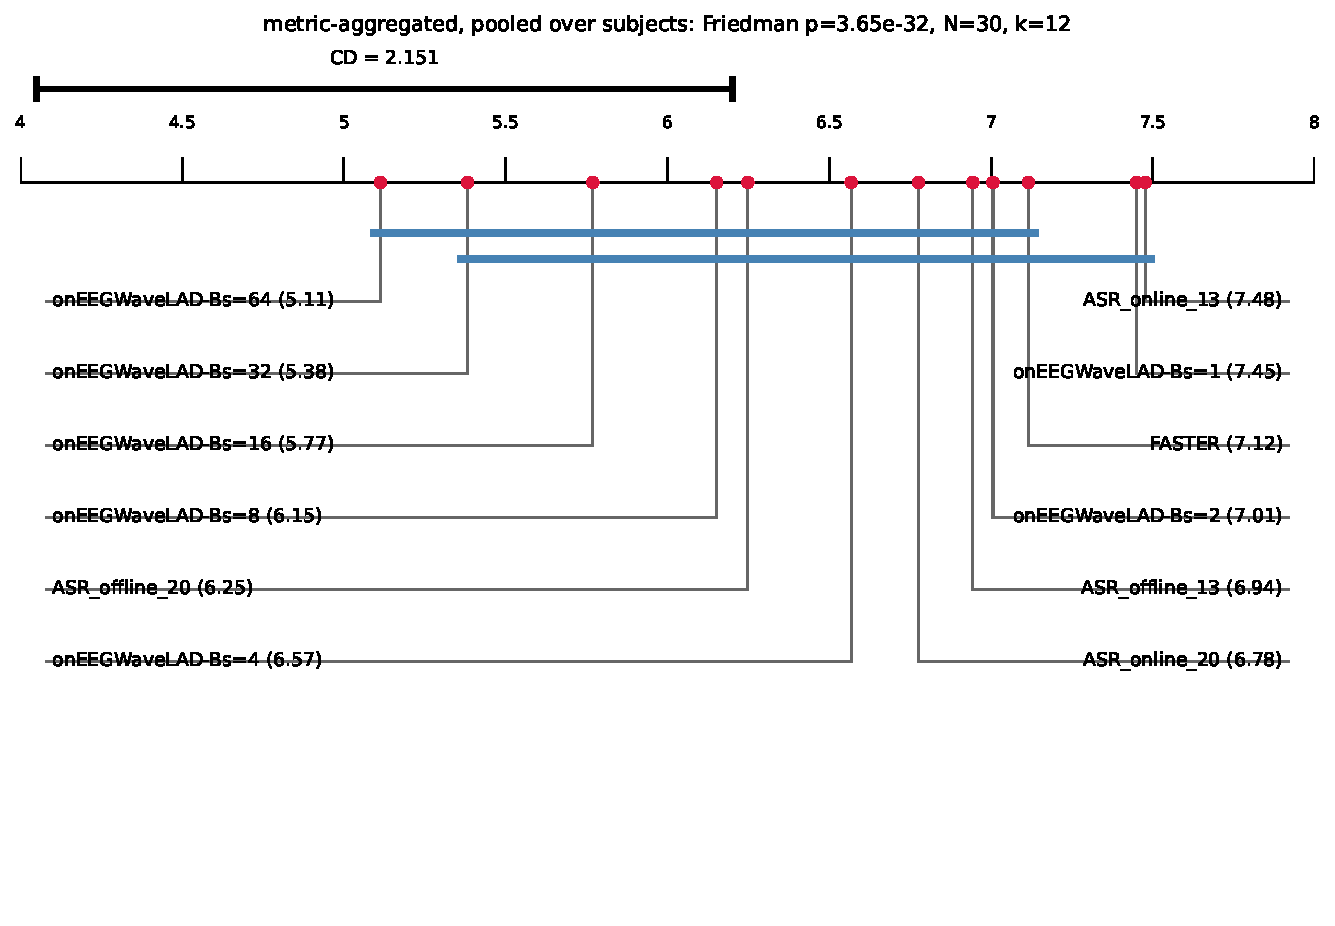
\includegraphics[width=0.95\textwidth]{Figures/CD_baseline_metric-aggregated_pooled.pdf}
\vspace{0.5em}
\hrule
\caption{Twelve-method comparison, metric-aggregated pooled view.}
\label{fig:cd_baseline_pooled}
\vspace{0.5em}
\hrule
\end{figure}

\begin{figure}[!htb]
\hrule
\vspace{0.5em}
\centering
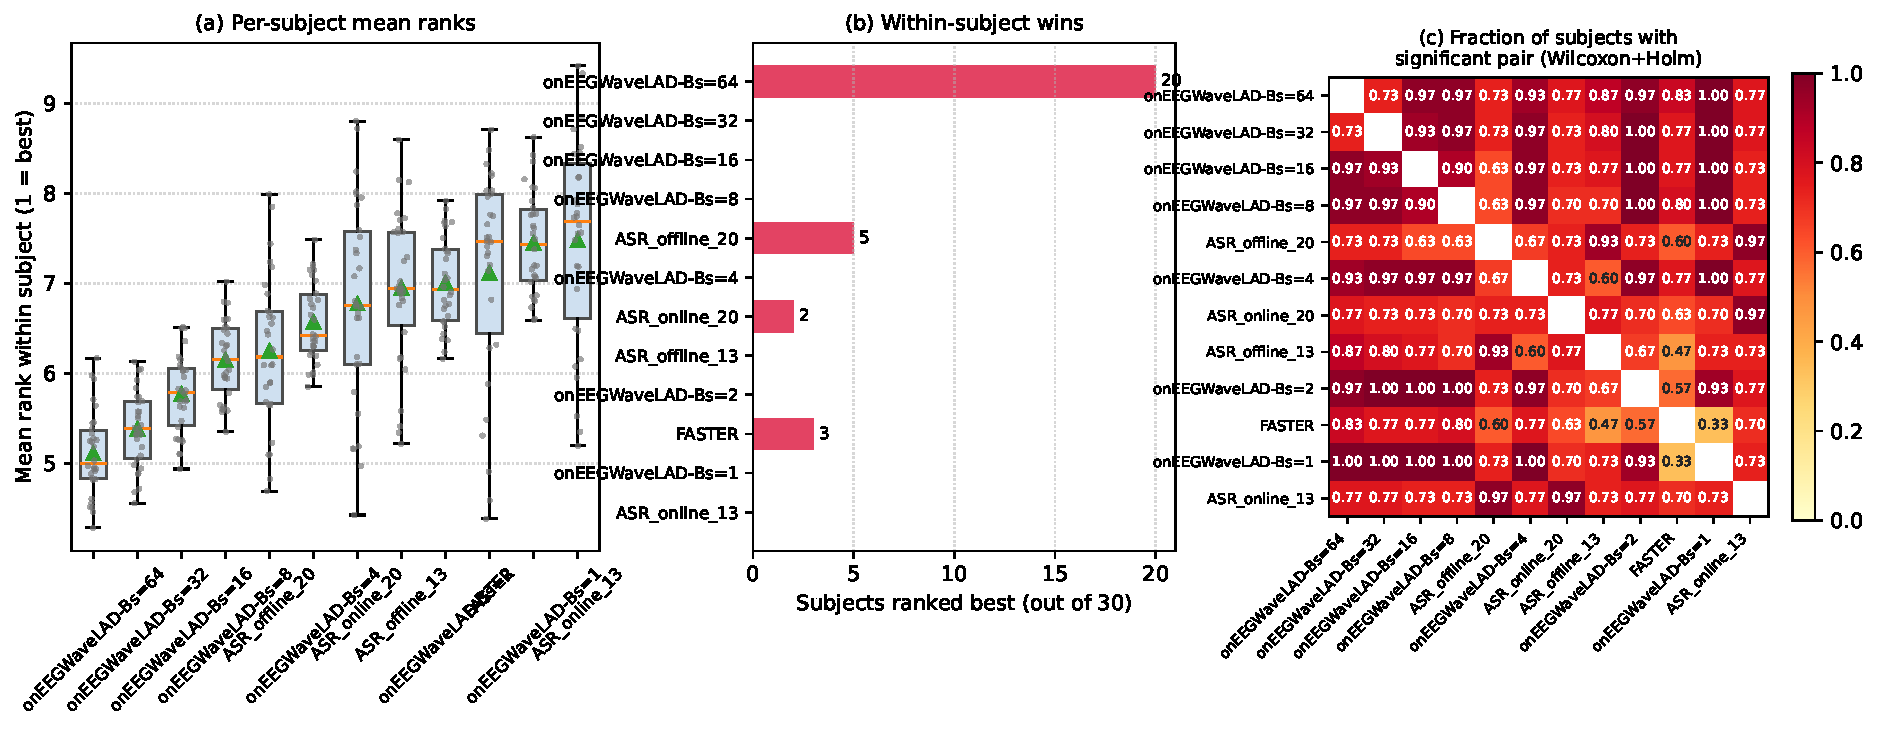
\includegraphics[width=\textwidth]{Figures/CD_baseline_metric-aggregated_summary.pdf}
\vspace{0.5em}
\hrule
\caption{Twelve-method comparison, summary statistics: (a) boxplot of ranks; (b) mean rank trajectory; (c) pairwise critical difference matrix.}
\label{fig:cd_baseline_summary}
\vspace{0.5em}
\hrule
\end{figure}

\begin{figure}[!htb]
\hrule
\vspace{0.5em}
\centering
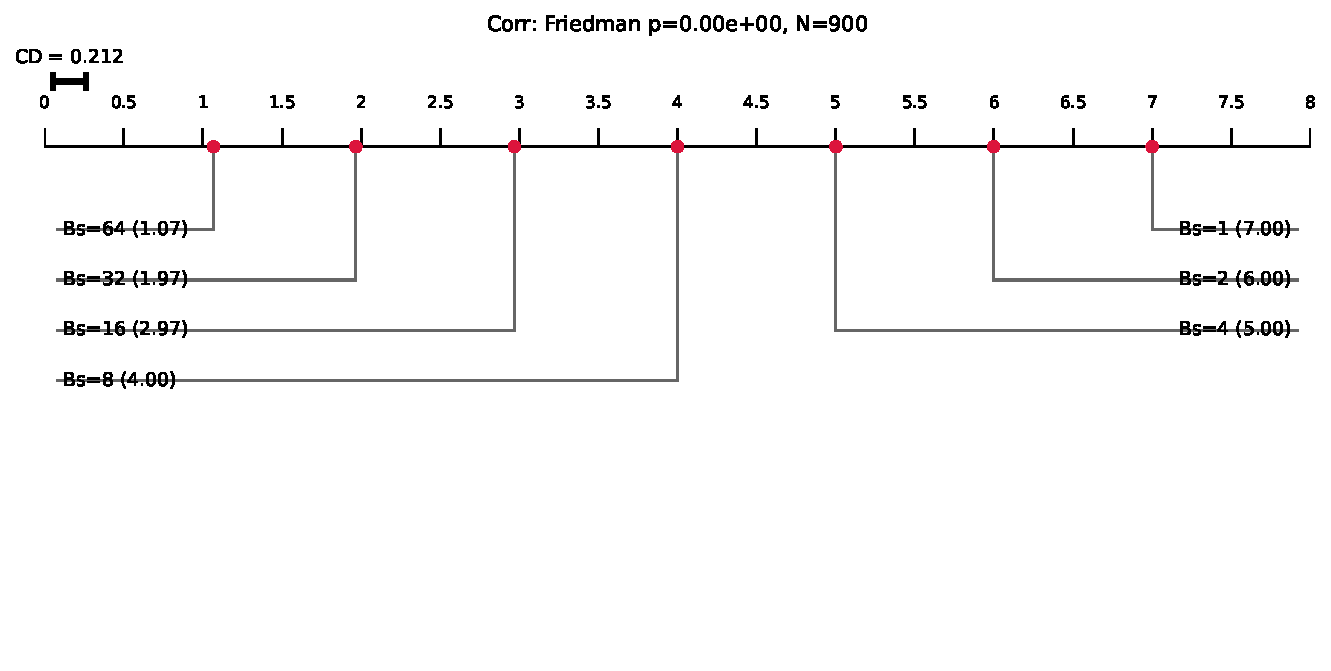
\includegraphics[width=0.85\textwidth]{Figures/CD_Bs_metric_Corr.pdf}
\vspace{0.5em}
\hrule
\caption{Single-metric CD: Pearson Correlation (CC), seven-buffer comparison. Similarity-oriented metric, monotonically improving with buffer size.}
\label{fig:cd_bs_cc}
\vspace{0.5em}
\hrule
\end{figure}

\begin{figure}[!htb]
\hrule
\vspace{0.5em}
\centering
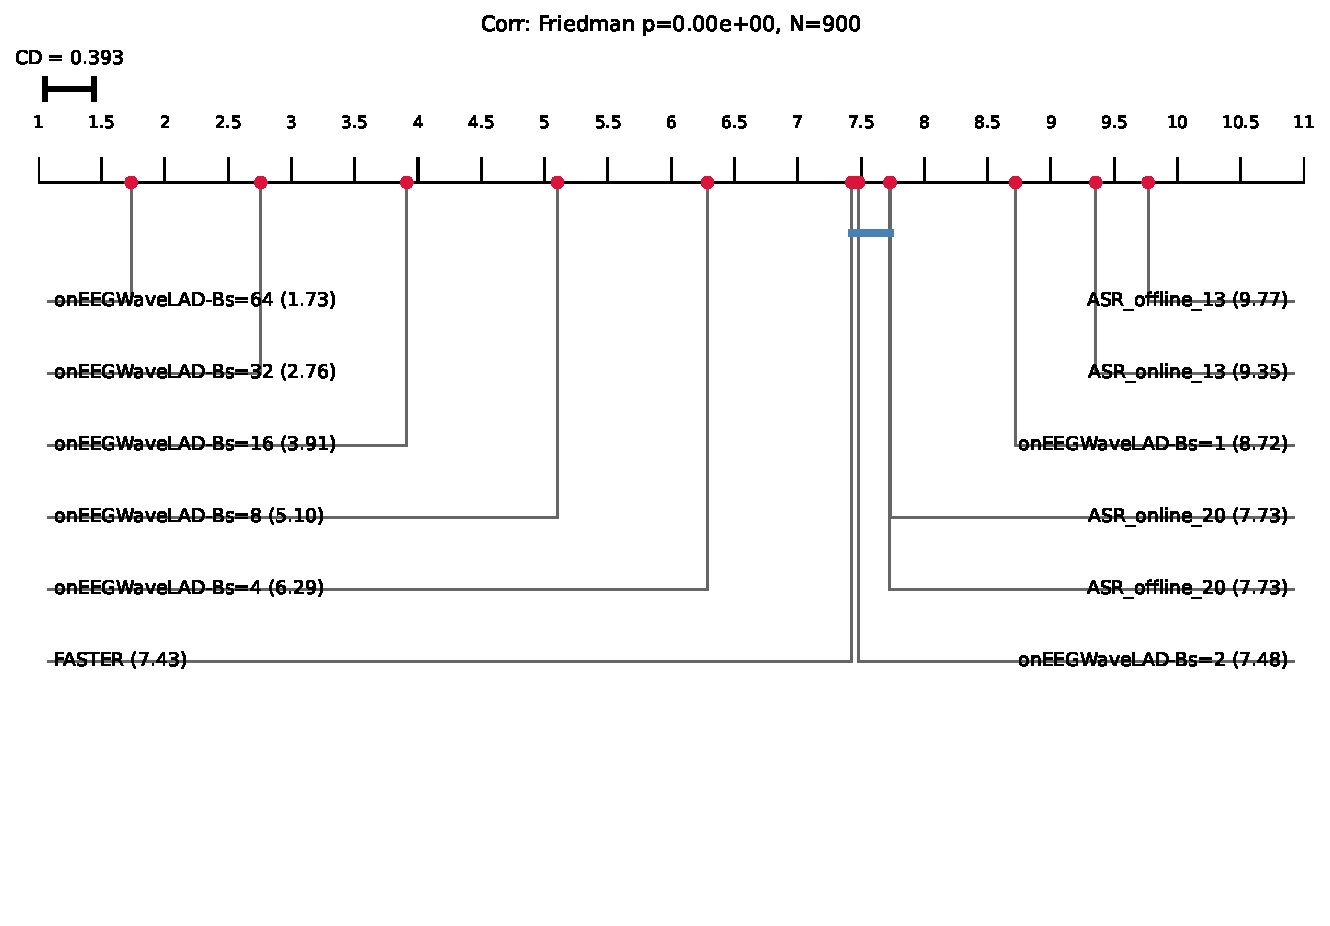
\includegraphics[width=0.95\textwidth]{Figures/CD_baseline_metric_Corr.pdf}
\vspace{0.5em}
\hrule
\caption{Single-metric CD: Pearson Correlation (CC), twelve-method comparison.}
\label{fig:cd_baseline_cc}
\vspace{0.5em}
\hrule
\end{figure}

\begin{figure}[!htb]
\hrule
\vspace{0.5em}
\centering
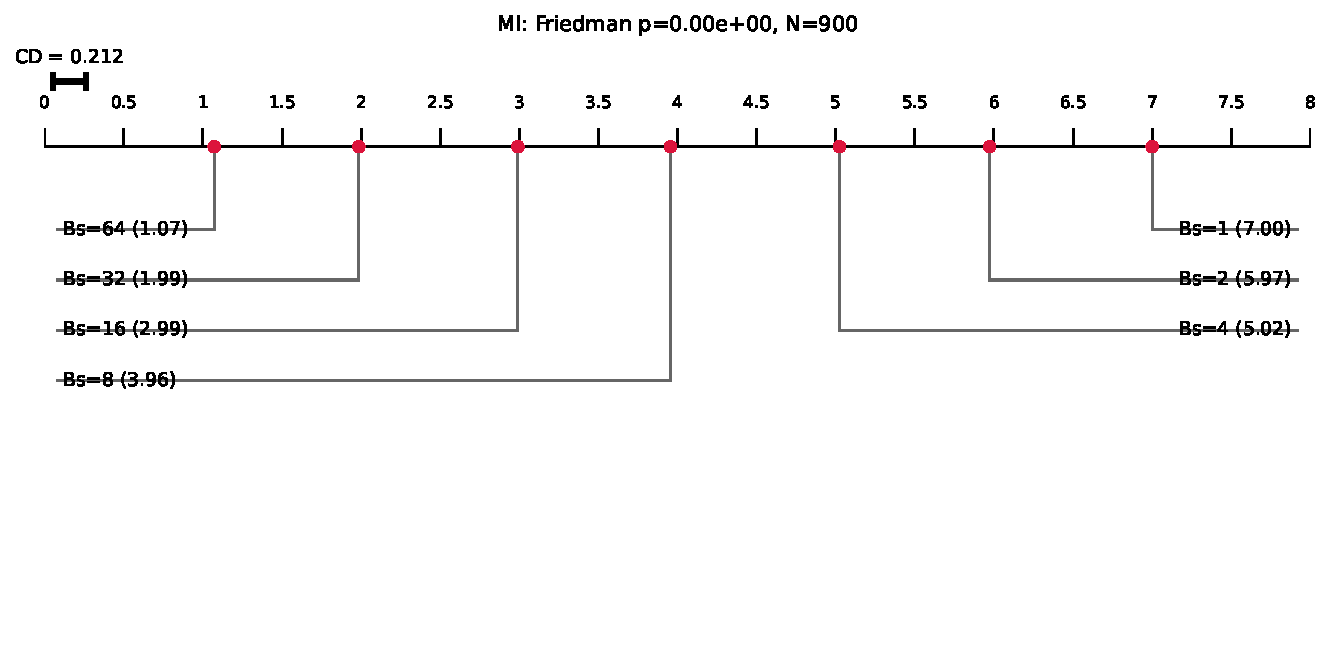
\includegraphics[width=0.85\textwidth]{Figures/CD_Bs_metric_MI.pdf}
\vspace{0.5em}
\hrule
\caption{Single-metric CD: Mutual Information (MI), seven-buffer comparison. Similarity-oriented metric, monotonically improving with buffer size.}
\label{fig:cd_bs_mi}
\vspace{0.5em}
\hrule
\end{figure}

\begin{figure}[!htb]
\hrule
\vspace{0.5em}
\centering
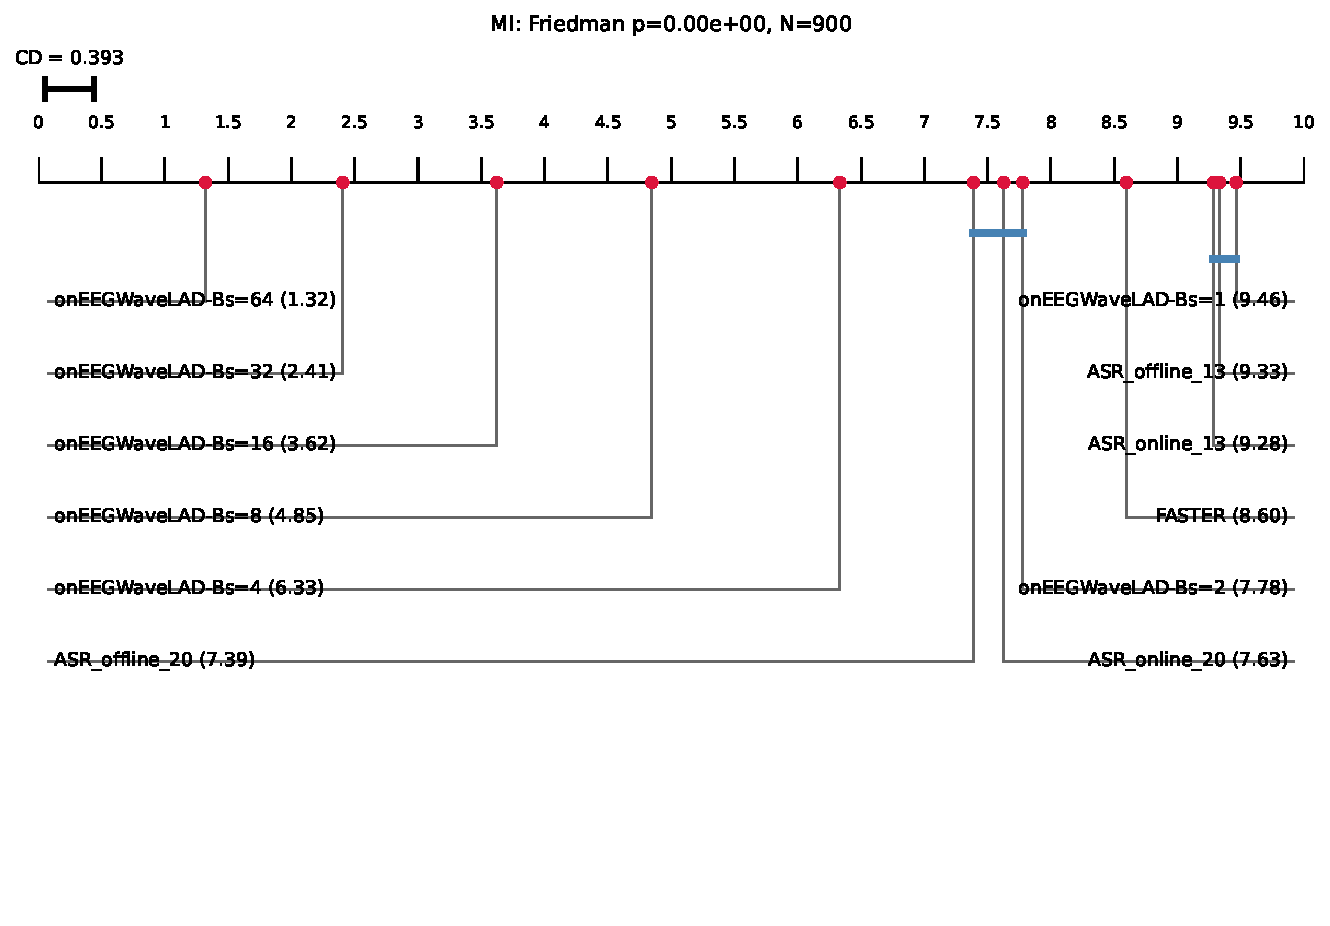
\includegraphics[width=0.95\textwidth]{Figures/CD_baseline_metric_MI.pdf}
\vspace{0.5em}
\hrule
\caption{Single-metric CD: Mutual Information (MI), twelve-method comparison.}
\label{fig:cd_baseline_mi}
\vspace{0.5em}
\hrule
\end{figure}

\begin{figure}[!htb]
\hrule
\vspace{0.5em}
\centering
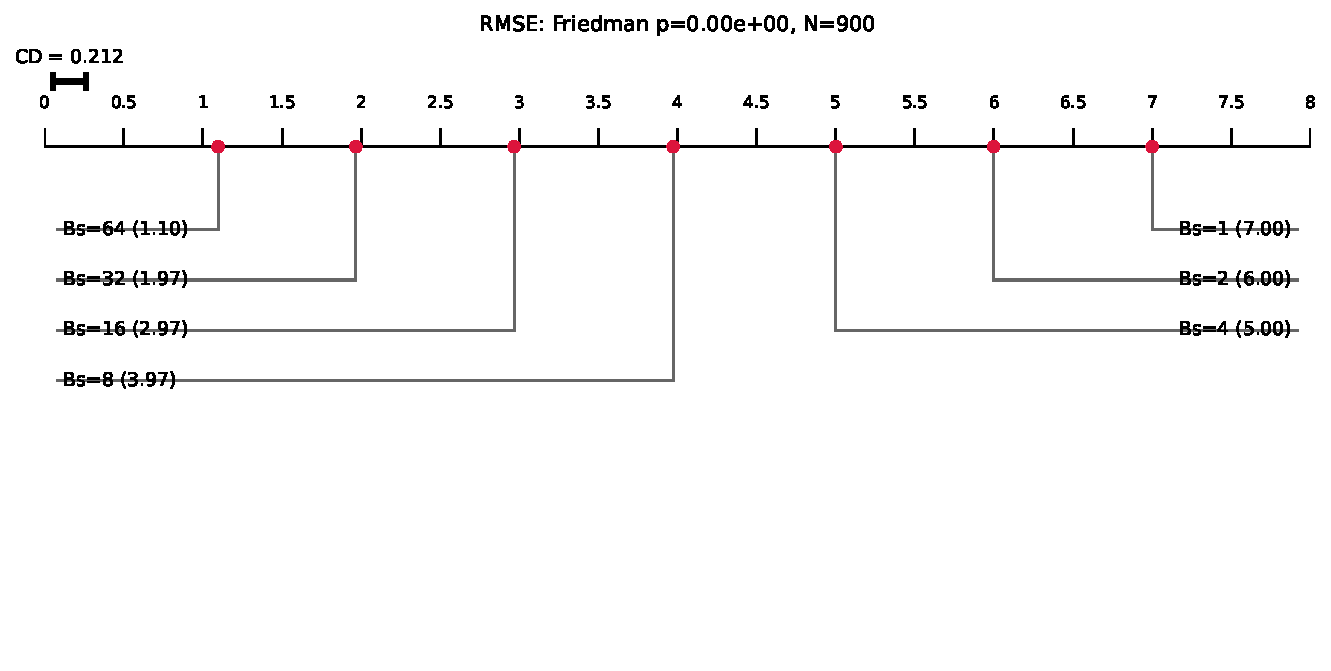
\includegraphics[width=0.85\textwidth]{Figures/CD_Bs_metric_RMSE.pdf}
\vspace{0.5em}
\hrule
\caption{Single-metric CD: Root Mean Square Error (RMSE), seven-buffer comparison. Similarity-oriented metric, monotonically decreasing (improving) with buffer size.}
\label{fig:cd_bs_rmse}
\vspace{0.5em}
\hrule
\end{figure}

\begin{figure}[!htb]
\hrule
\vspace{0.5em}
\centering
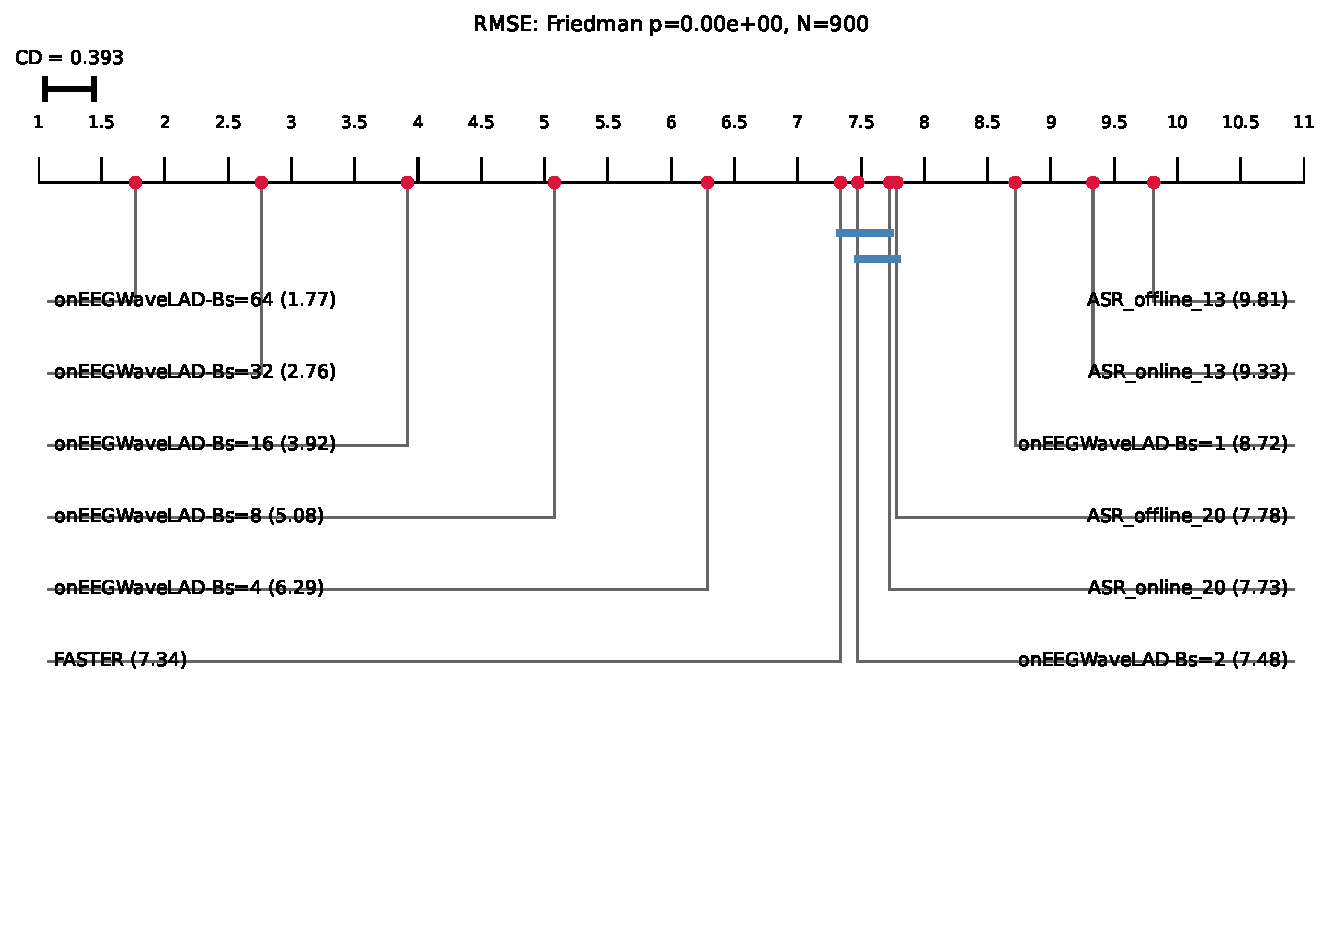
\includegraphics[width=0.95\textwidth]{Figures/CD_baseline_metric_RMSE.pdf}
\vspace{0.5em}
\hrule
\caption{Single-metric CD: RMSE, twelve-method comparison.}
\label{fig:cd_baseline_rmse}
\vspace{0.5em}
\hrule
\end{figure}

\begin{figure}[!htb]
\hrule
\vspace{0.5em}
\centering
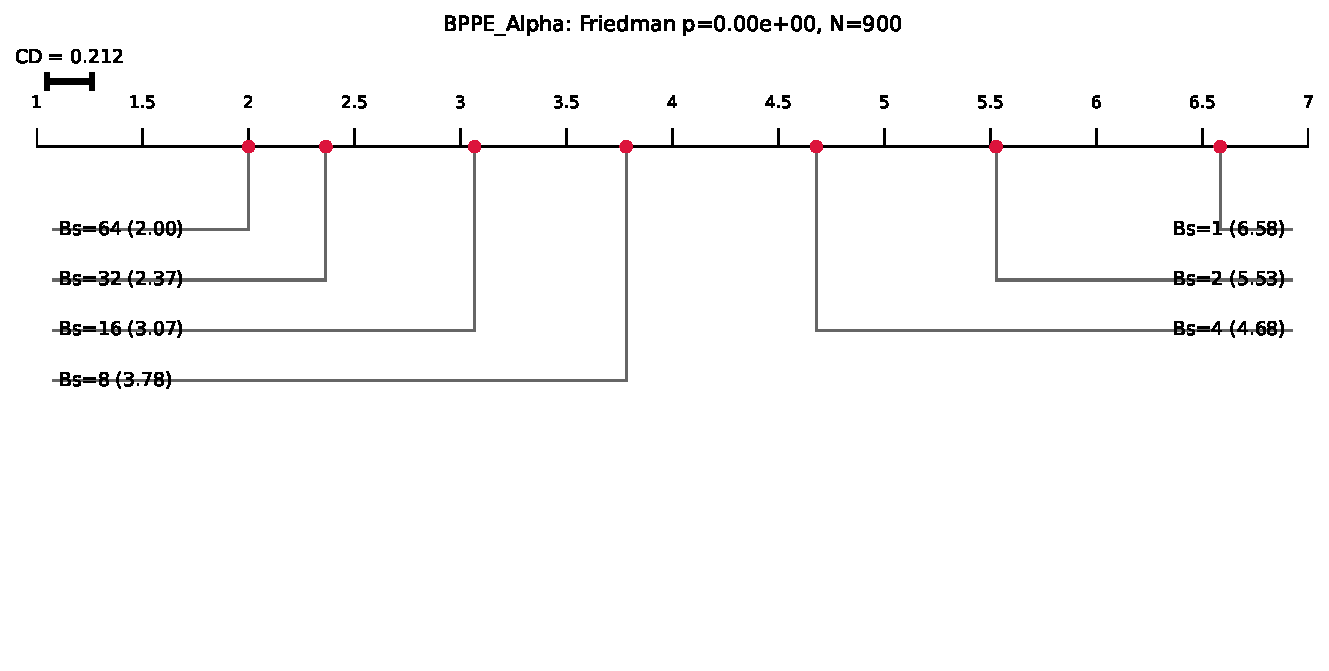
\includegraphics[width=0.85\textwidth]{Figures/CD_Bs_metric_BPPE_Alpha.pdf}
\vspace{0.5em}
\hrule
\caption{Single-metric CD: BPPE Alpha Band, seven-buffer comparison. Similarity-oriented metric, monotonically improving with buffer size.}
\label{fig:cd_bs_bppe_alpha}
\vspace{0.5em}
\hrule
\end{figure}

\begin{figure}[!htb]
\hrule
\vspace{0.5em}
\centering
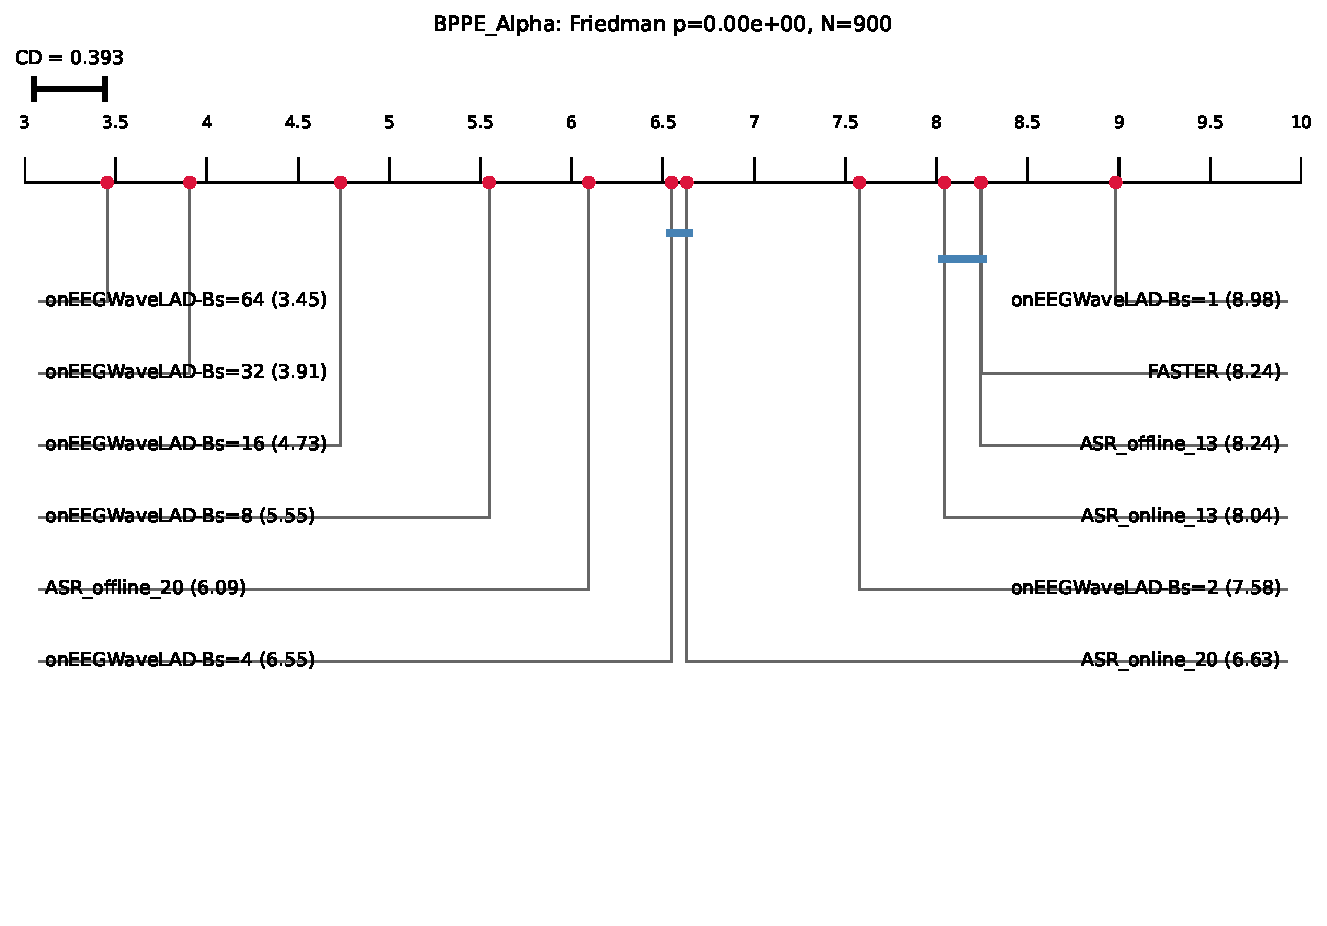
\includegraphics[width=0.95\textwidth]{Figures/CD_baseline_metric_BPPE_Alpha.pdf}
\vspace{0.5em}
\hrule
\caption{Single-metric CD: BPPE Alpha Band, twelve-method comparison.}
\label{fig:cd_baseline_bppe_alpha}
\vspace{0.5em}
\hrule
\end{figure}

\begin{figure}[!htb]
\hrule
\vspace{0.5em}
\centering
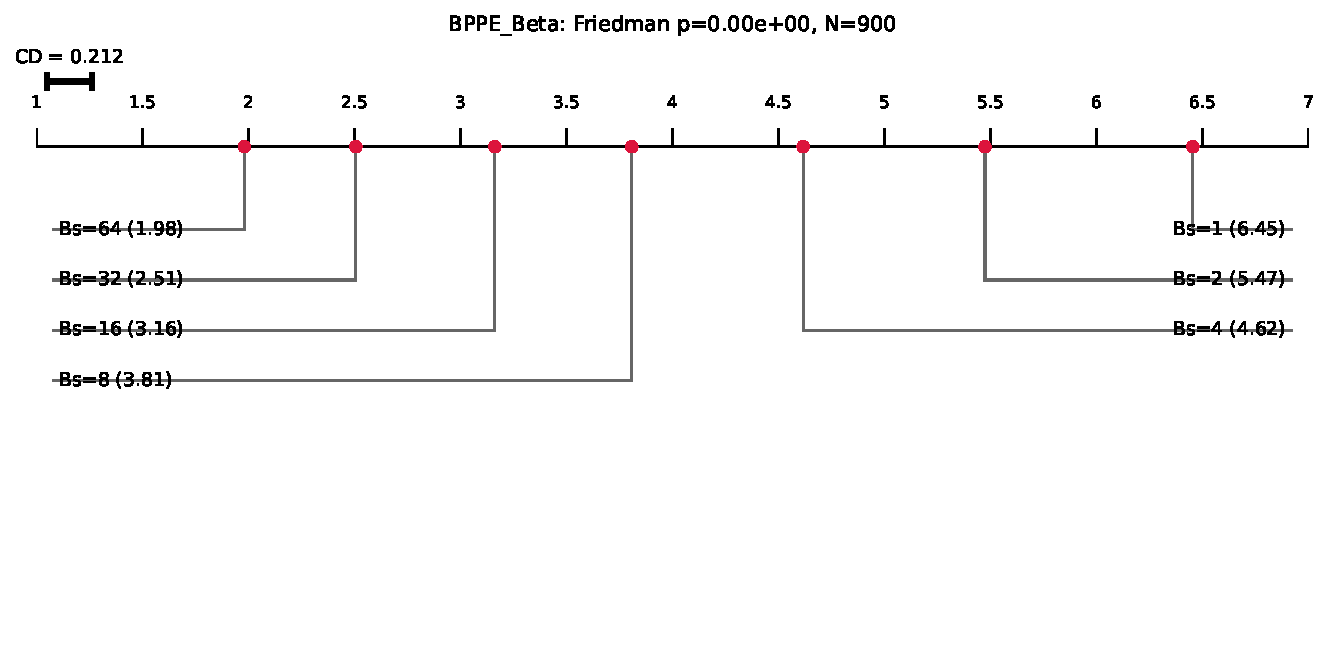
\includegraphics[width=0.85\textwidth]{Figures/CD_Bs_metric_BPPE_Beta.pdf}
\vspace{0.5em}
\hrule
\caption{Single-metric CD: BPPE Beta Band, seven-buffer comparison. Similarity-oriented metric, monotonically improving with buffer size.}
\label{fig:cd_bs_bppe_beta}
\vspace{0.5em}
\hrule
\end{figure}

\begin{figure}[!htb]
\hrule
\vspace{0.5em}
\centering
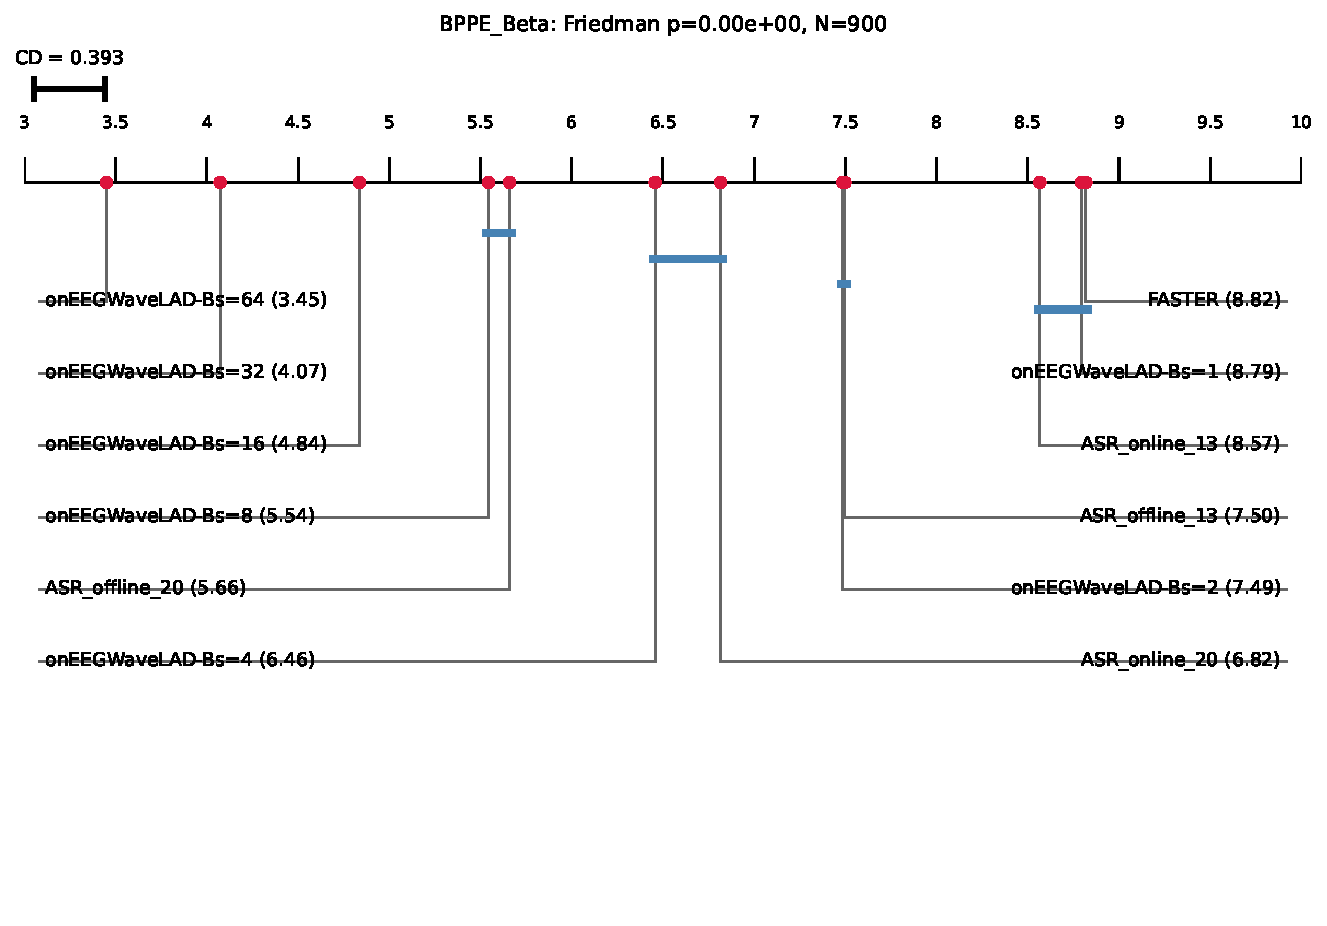
\includegraphics[width=0.95\textwidth]{Figures/CD_baseline_metric_BPPE_Beta.pdf}
\vspace{0.5em}
\hrule
\caption{Single-metric CD: BPPE Beta Band, twelve-method comparison.}
\label{fig:cd_baseline_bppe_beta}
\vspace{0.5em}
\hrule
\end{figure}

\begin{figure}[!htb]
\hrule
\vspace{0.5em}
\centering
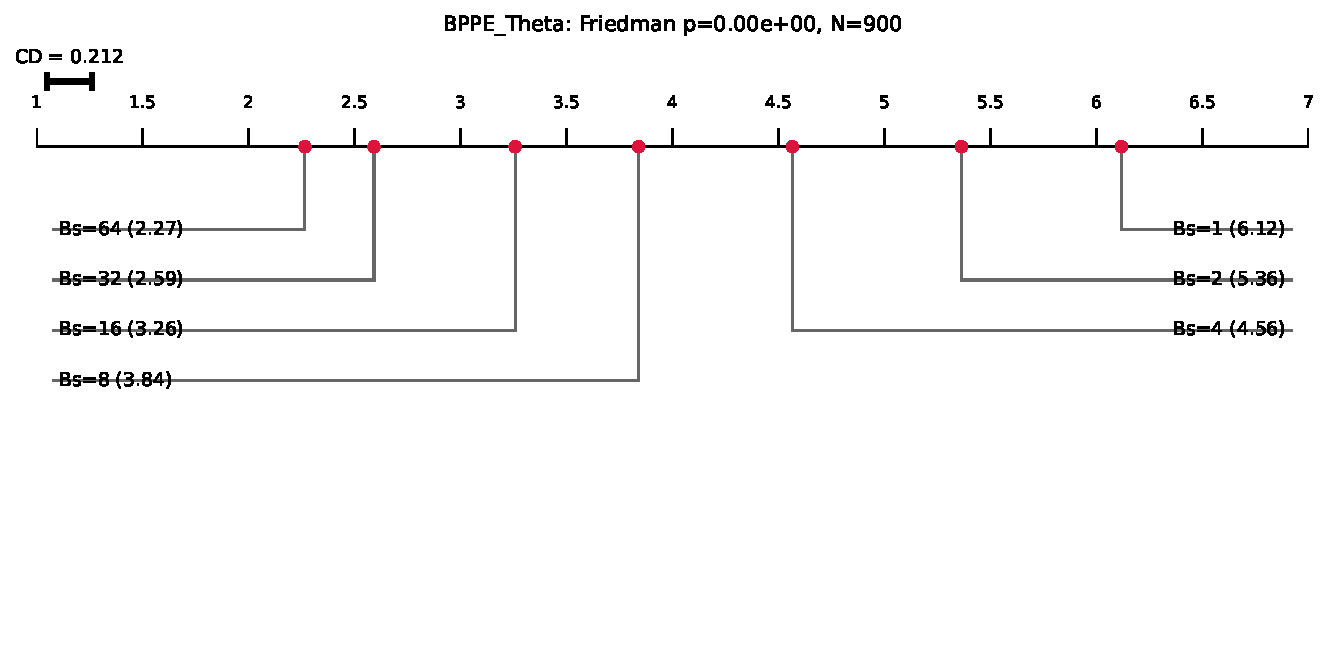
\includegraphics[width=0.85\textwidth]{Figures/CD_Bs_metric_BPPE_Theta.pdf}
\vspace{0.5em}
\hrule
\caption{Single-metric CD: BPPE Theta Band, seven-buffer comparison. Similarity-oriented metric, monotonically improving with buffer size.}
\label{fig:cd_bs_bppe_theta}
\vspace{0.5em}
\hrule
\end{figure}

\begin{figure}[!htb]
\hrule
\vspace{0.5em}
\centering
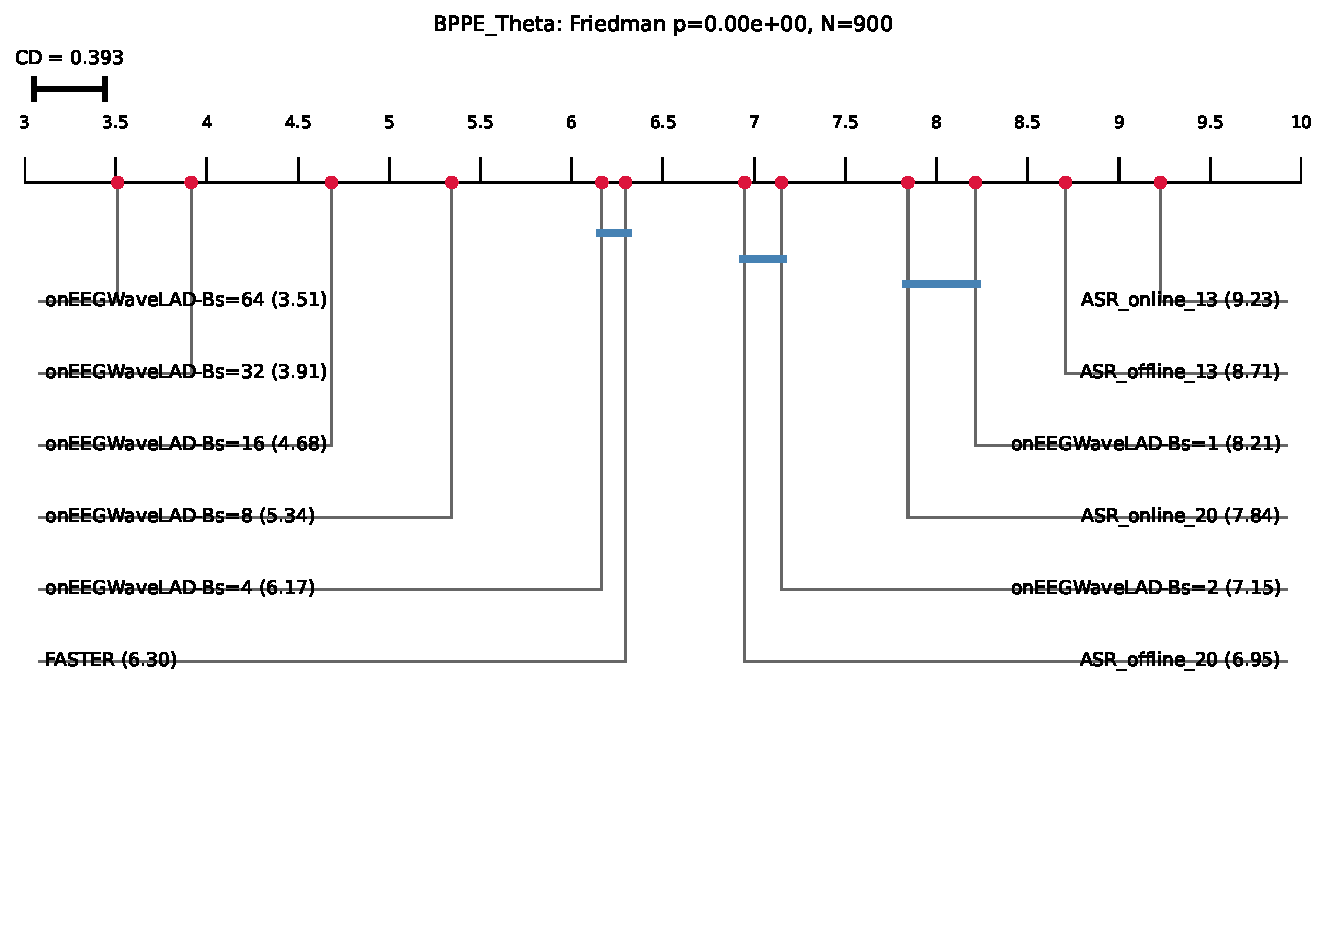
\includegraphics[width=0.95\textwidth]{Figures/CD_baseline_metric_BPPE_Theta.pdf}
\vspace{0.5em}
\hrule
\caption{Single-metric CD: BPPE Theta Band, twelve-method comparison.}
\label{fig:cd_baseline_bppe_theta}
\vspace{0.5em}
\hrule
\end{figure}

\begin{figure}[!htb]
\hrule
\vspace{0.5em}
\centering
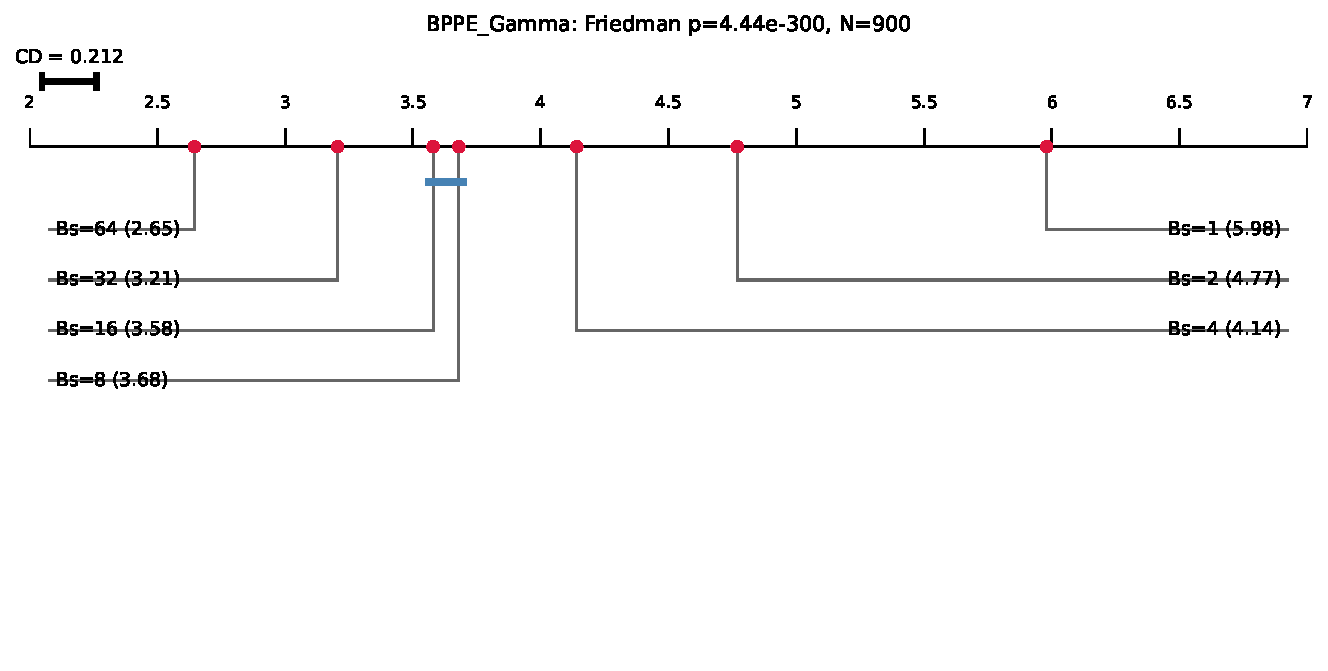
\includegraphics[width=0.85\textwidth]{Figures/CD_Bs_metric_BPPE_Gamma.pdf}
\vspace{0.5em}
\hrule
\caption{Single-metric CD: BPPE Gamma Band, seven-buffer comparison. Similarity-oriented metric, monotonically improving with buffer size.}
\label{fig:cd_bs_bppe_gamma}
\vspace{0.5em}
\hrule
\end{figure}

\begin{figure}[!htb]
\hrule
\vspace{0.5em}
\centering
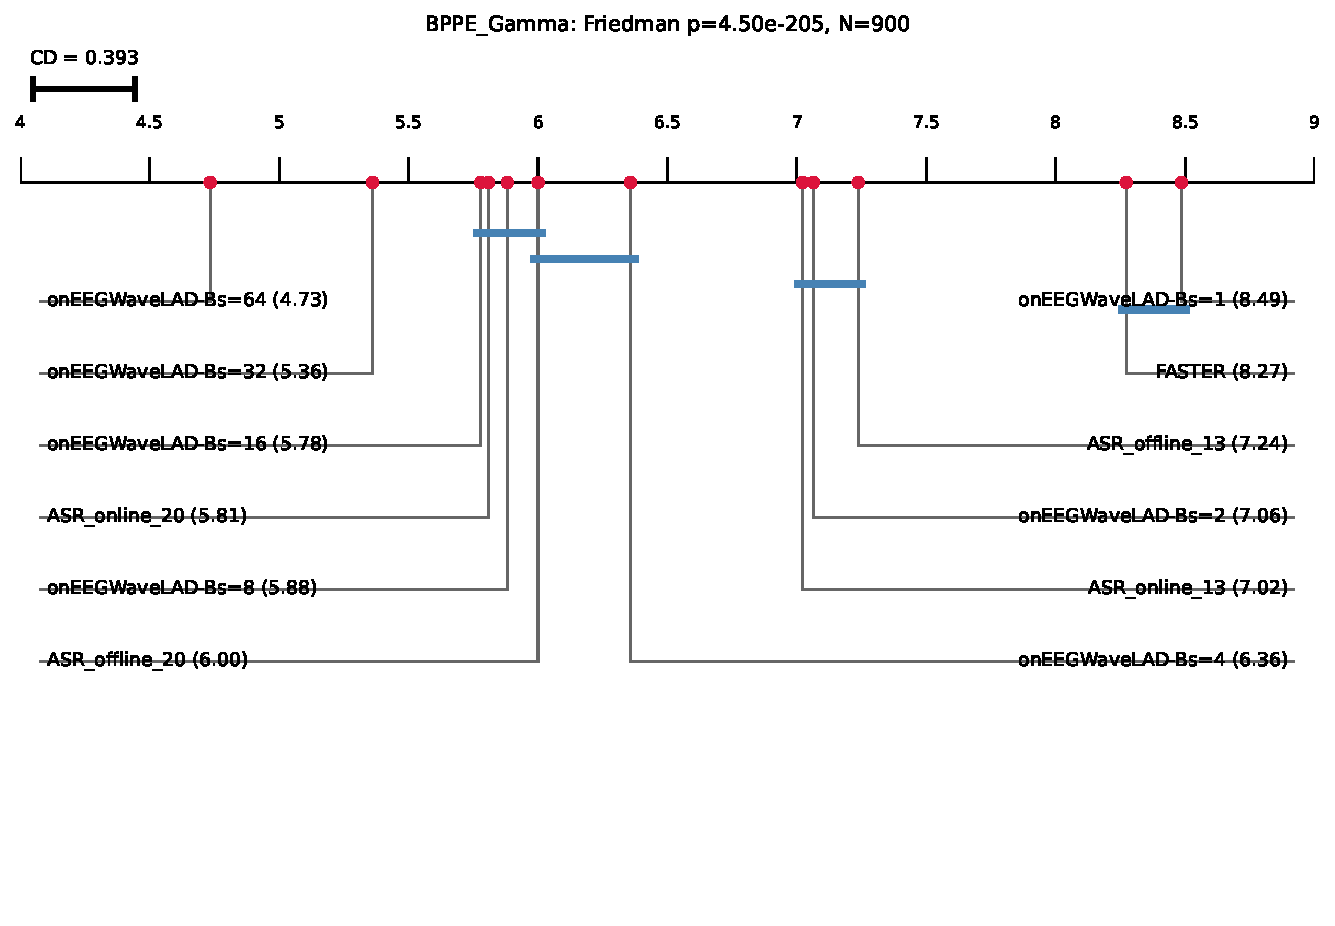
\includegraphics[width=0.95\textwidth]{Figures/CD_baseline_metric_BPPE_Gamma.pdf}
\vspace{0.5em}
\hrule
\caption{Single-metric CD: BPPE Gamma Band, twelve-method comparison.}
\label{fig:cd_baseline_bppe_gamma}
\vspace{0.5em}
\hrule
\end{figure}

\begin{figure}[!htb]
\hrule
\vspace{0.5em}
\centering
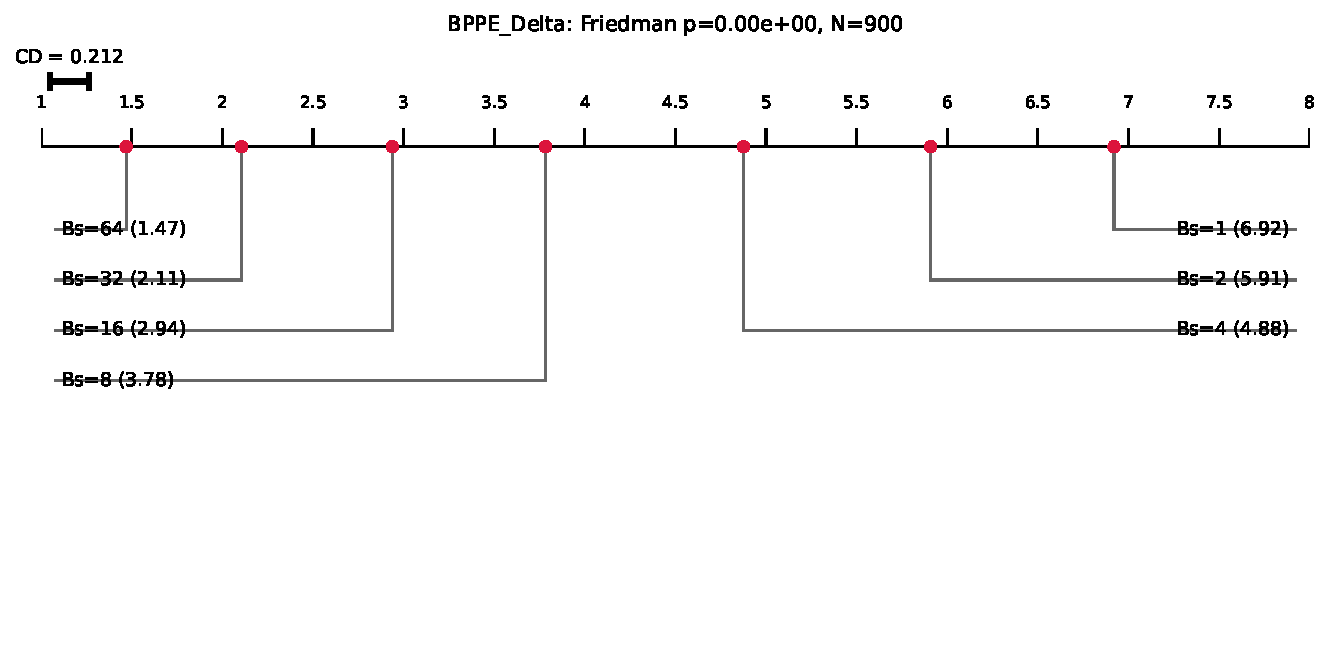
\includegraphics[width=0.85\textwidth]{Figures/CD_Bs_metric_BPPE_Delta.pdf}
\vspace{0.5em}
\hrule
\caption{Single-metric CD: BPPE Delta Band, seven-buffer comparison. Similarity-oriented metric, monotonically improving with buffer size.}
\label{fig:cd_bs_bppe_delta}
\vspace{0.5em}
\hrule
\end{figure}

\begin{figure}[!htb]
\hrule
\vspace{0.5em}
\centering
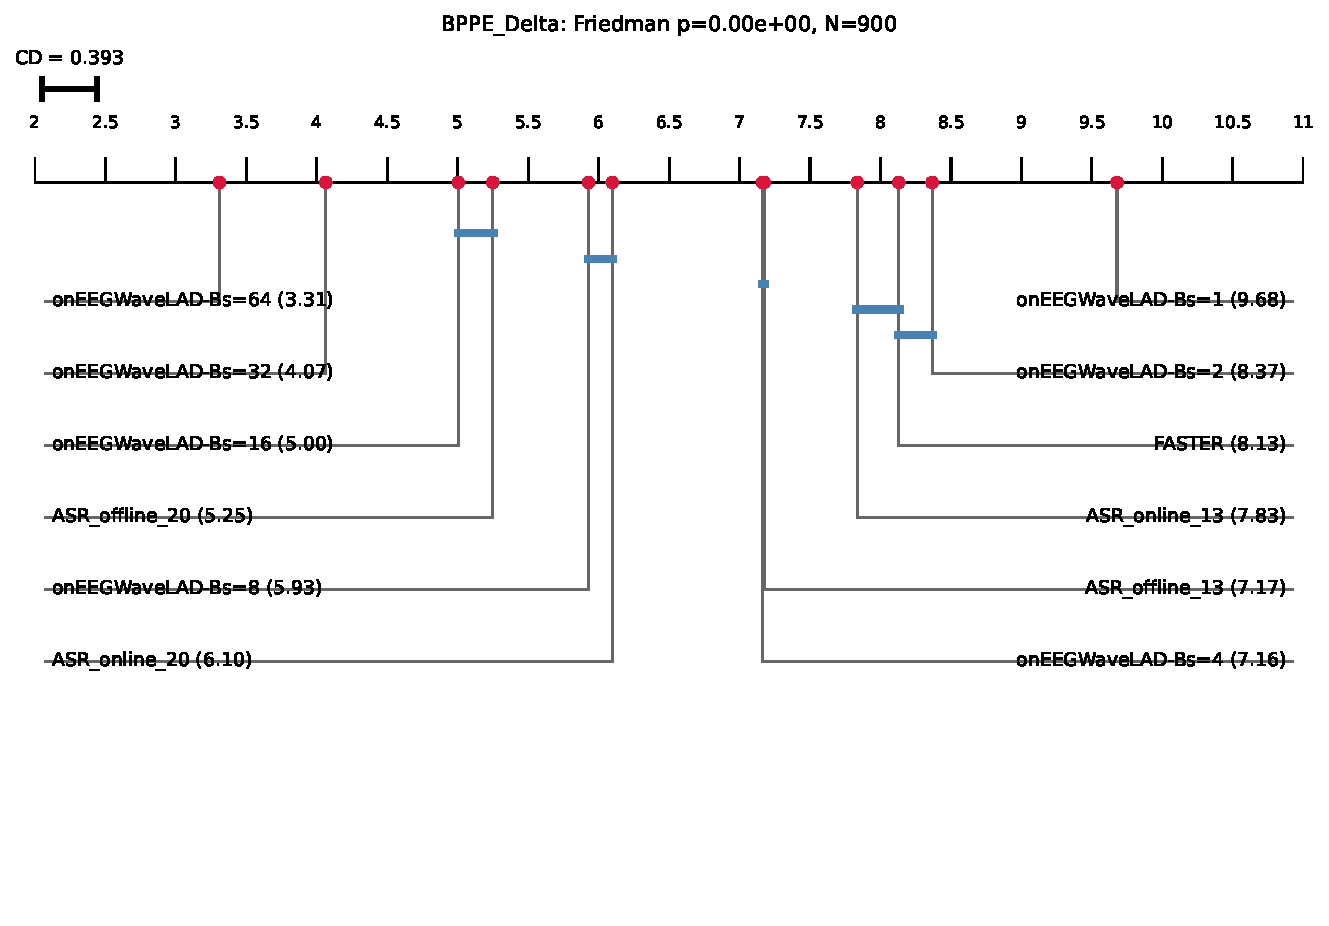
\includegraphics[width=0.95\textwidth]{Figures/CD_baseline_metric_BPPE_Delta.pdf}
\vspace{0.5em}
\hrule
\caption{Single-metric CD: BPPE Delta Band, twelve-method comparison.}
\label{fig:cd_baseline_bppe_delta}
\vspace{0.5em}
\hrule
\end{figure}

\begin{figure}[!htb]
\hrule
\vspace{0.5em}
\centering
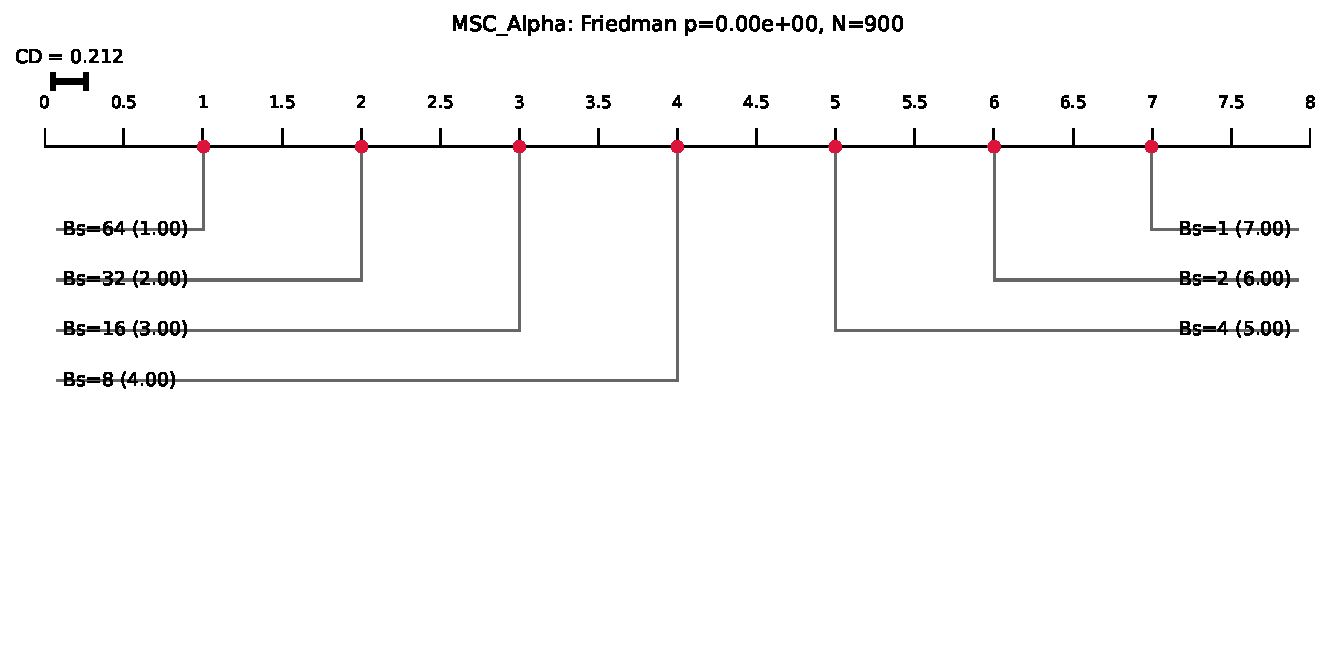
\includegraphics[width=0.85\textwidth]{Figures/CD_Bs_metric_MSC_Alpha.pdf}
\vspace{0.5em}
\hrule
\caption{Single-metric CD: MSC Alpha Band, seven-buffer comparison. Similarity-oriented metric, monotonically improving with buffer size.}
\label{fig:cd_bs_msc_alpha}
\vspace{0.5em}
\hrule
\end{figure}

\begin{figure}[!htb]
\hrule
\vspace{0.5em}
\centering
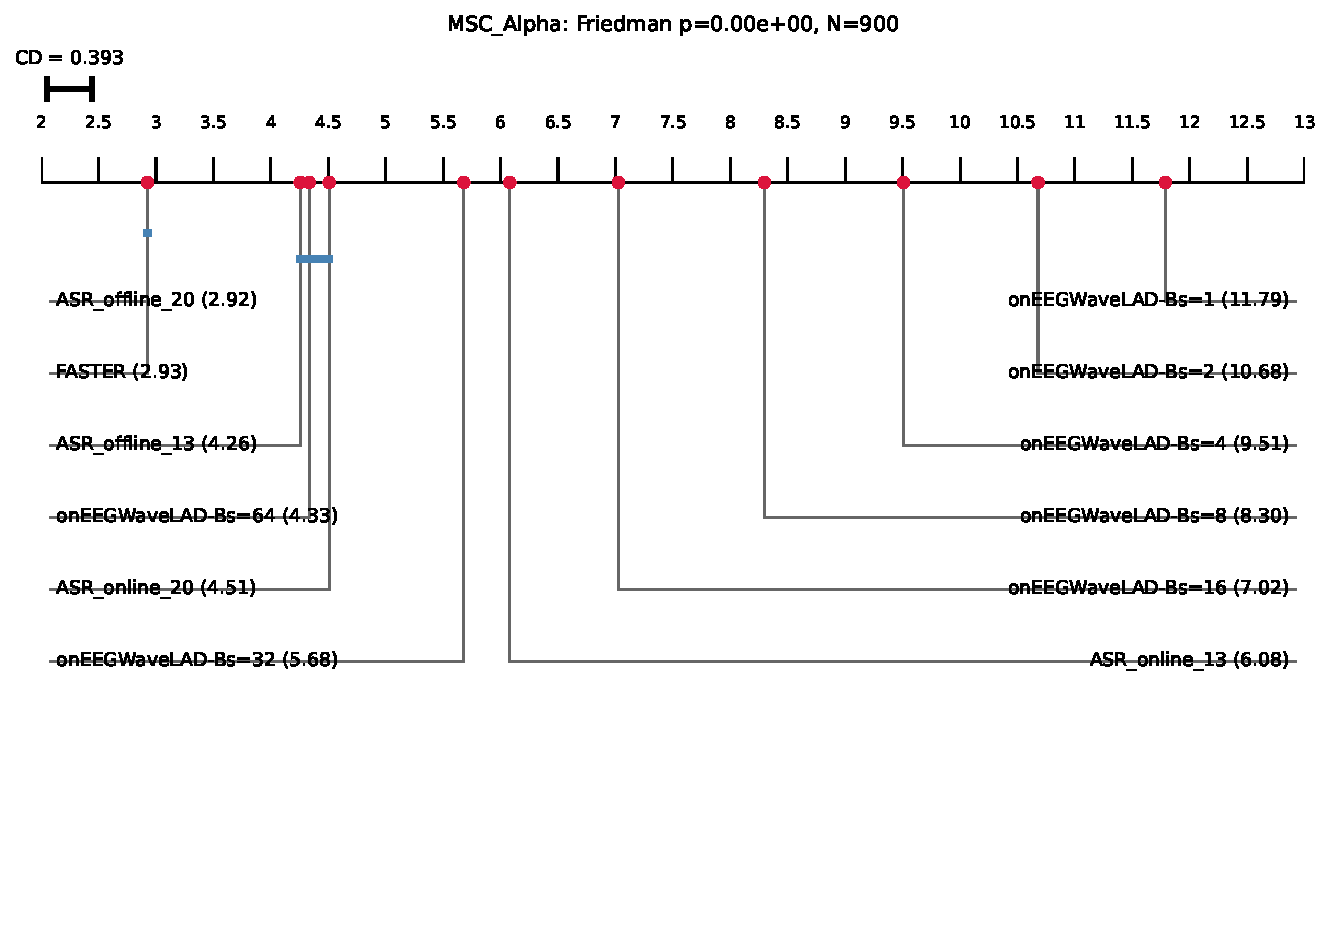
\includegraphics[width=0.95\textwidth]{Figures/CD_baseline_metric_MSC_Alpha.pdf}
\vspace{0.5em}
\hrule
\caption{Single-metric CD: MSC Alpha Band, twelve-method comparison.}
\label{fig:cd_baseline_msc_alpha}
\vspace{0.5em}
\hrule
\end{figure}

\begin{figure}[!htb]
\hrule
\vspace{0.5em}
\centering
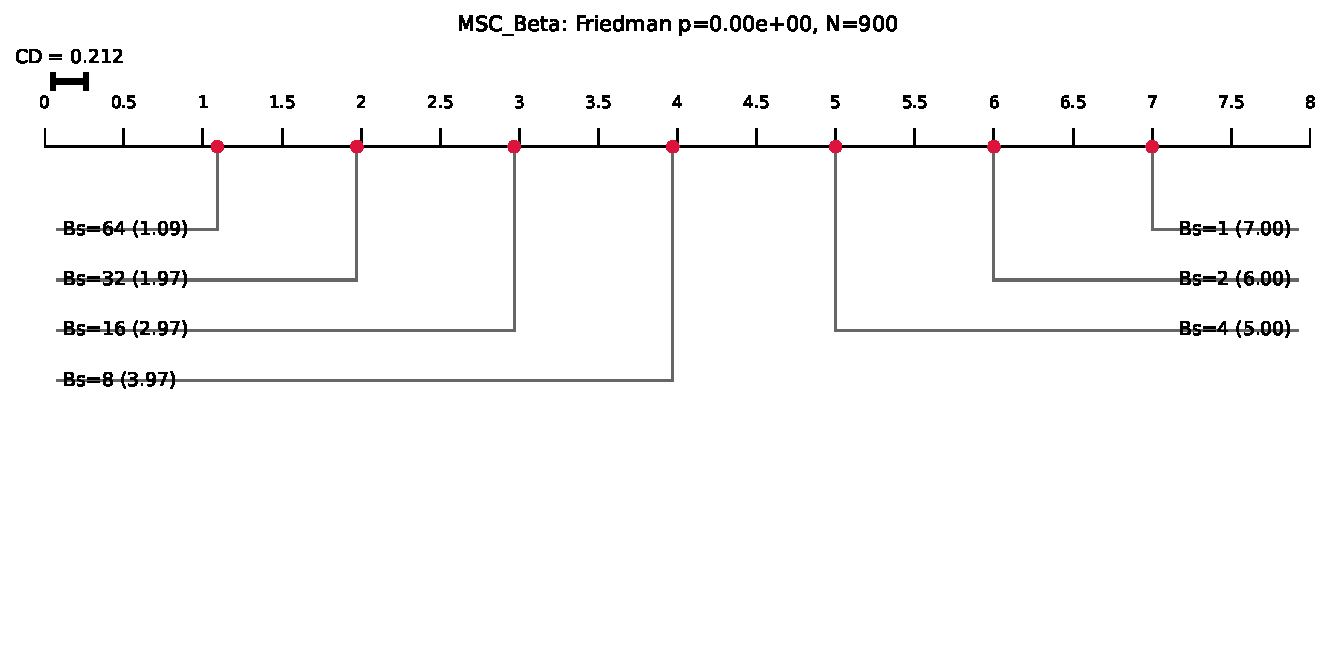
\includegraphics[width=0.85\textwidth]{Figures/CD_Bs_metric_MSC_Beta.pdf}
\vspace{0.5em}
\hrule
\caption{Single-metric CD: MSC Beta Band, seven-buffer comparison. Similarity-oriented metric, monotonically improving with buffer size.}
\label{fig:cd_bs_msc_beta}
\vspace{0.5em}
\hrule
\end{figure}

\begin{figure}[!htb]
\hrule
\vspace{0.5em}
\centering
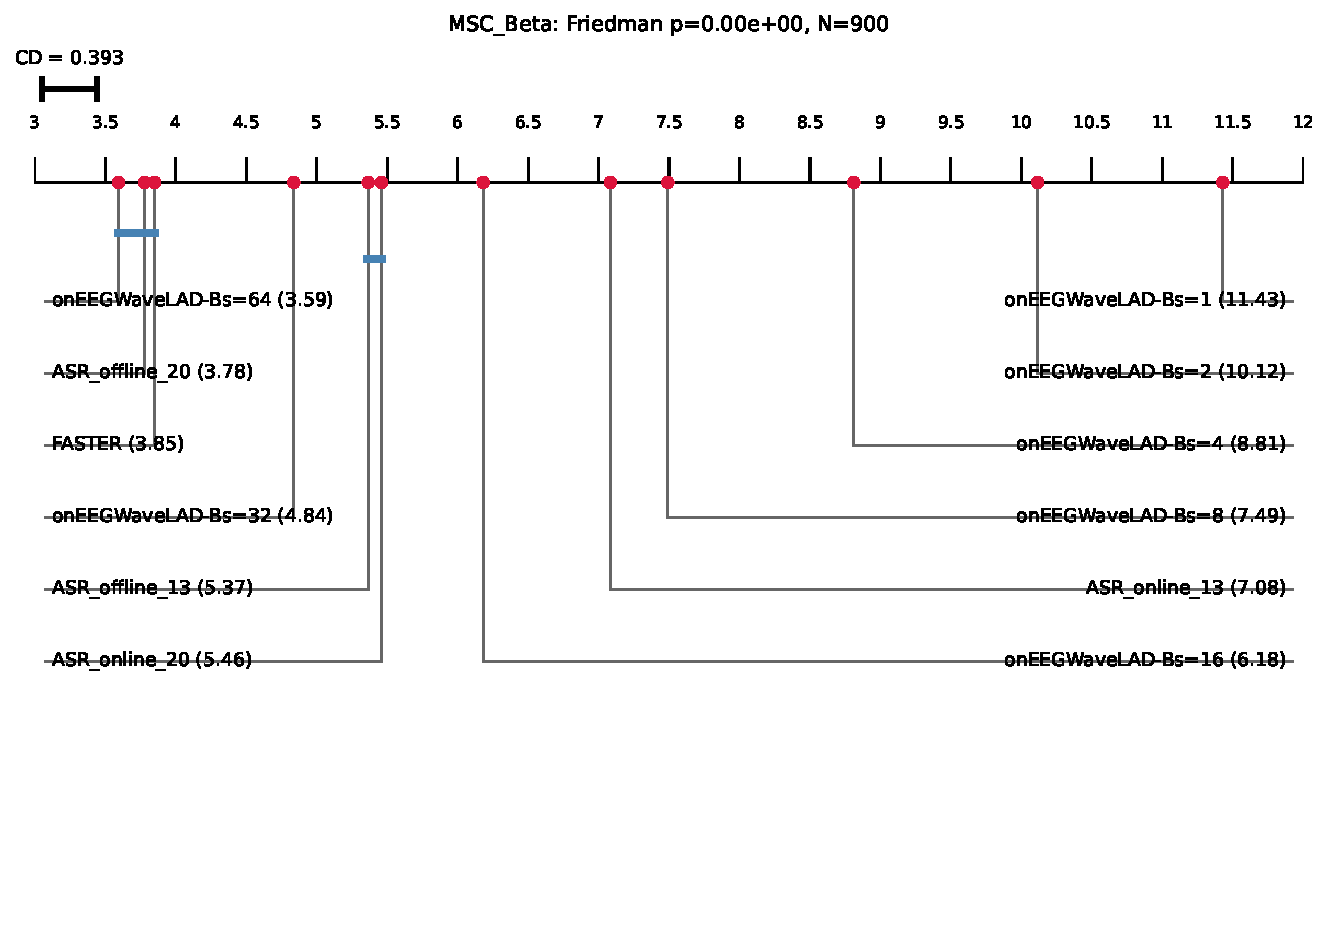
\includegraphics[width=0.95\textwidth]{Figures/CD_baseline_metric_MSC_Beta.pdf}
\vspace{0.5em}
\hrule
\caption{Single-metric CD: MSC Beta Band, twelve-method comparison.}
\label{fig:cd_baseline_msc_beta}
\vspace{0.5em}
\hrule
\end{figure}

\begin{figure}[!htb]
\hrule
\vspace{0.5em}
\centering
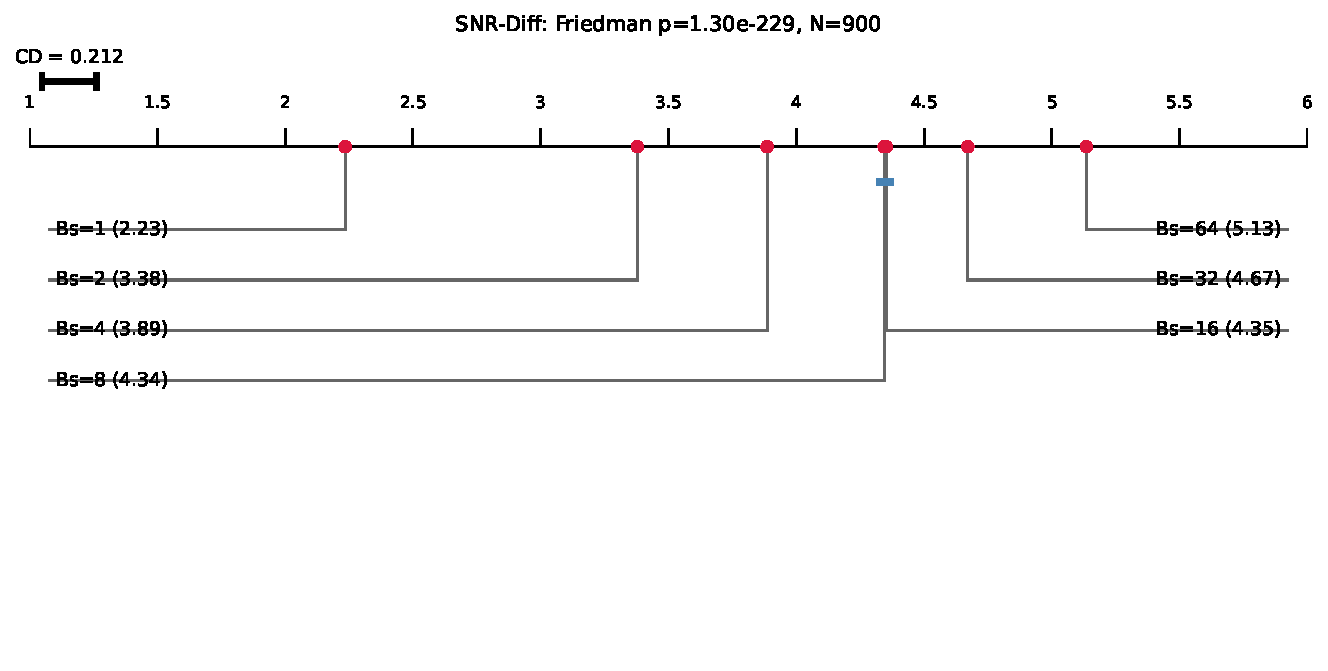
\includegraphics[width=0.85\textwidth]{Figures/CD_Bs_metric_SNR-Diff.pdf}
\vspace{0.5em}
\hrule
\caption{Single-metric CD: SNR-Diff, seven-buffer comparison. Artefact-removal metric, non-monotonic behaviour favouring smaller buffers.}
\label{fig:cd_bs_snr}
\vspace{0.5em}
\hrule
\end{figure}

\begin{figure}[!htb]
\hrule
\vspace{0.5em}
\centering
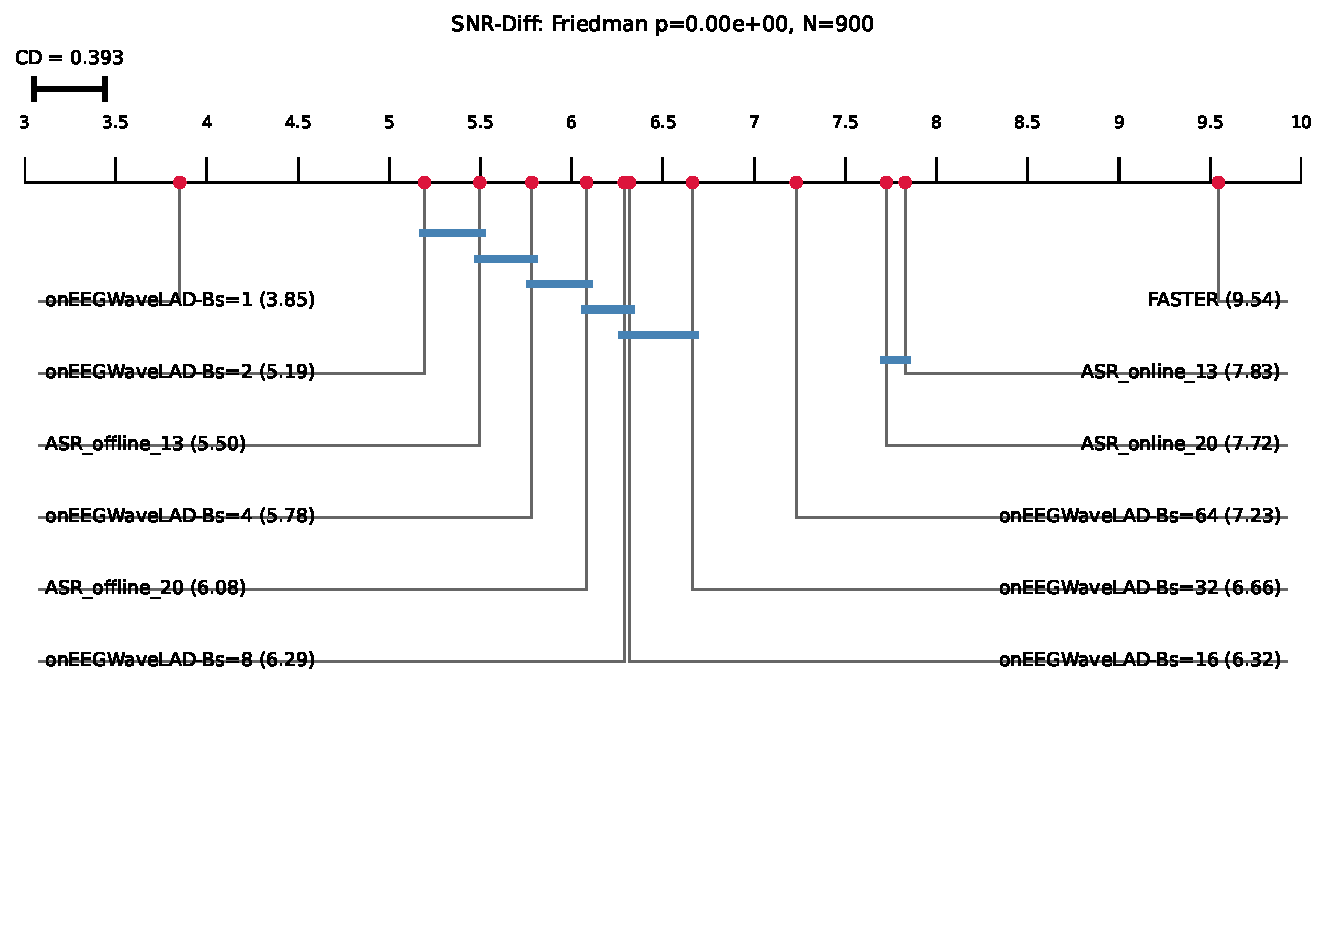
\includegraphics[width=0.95\textwidth]{Figures/CD_baseline_metric_SNR-Diff.pdf}
\vspace{0.5em}
\hrule
\caption{Single-metric CD: SNR-Diff, twelve-method comparison.}
\label{fig:cd_baseline_snr}
\vspace{0.5em}
\hrule
\end{figure}

\begin{figure}[!htb]
\hrule
\vspace{0.5em}
\centering
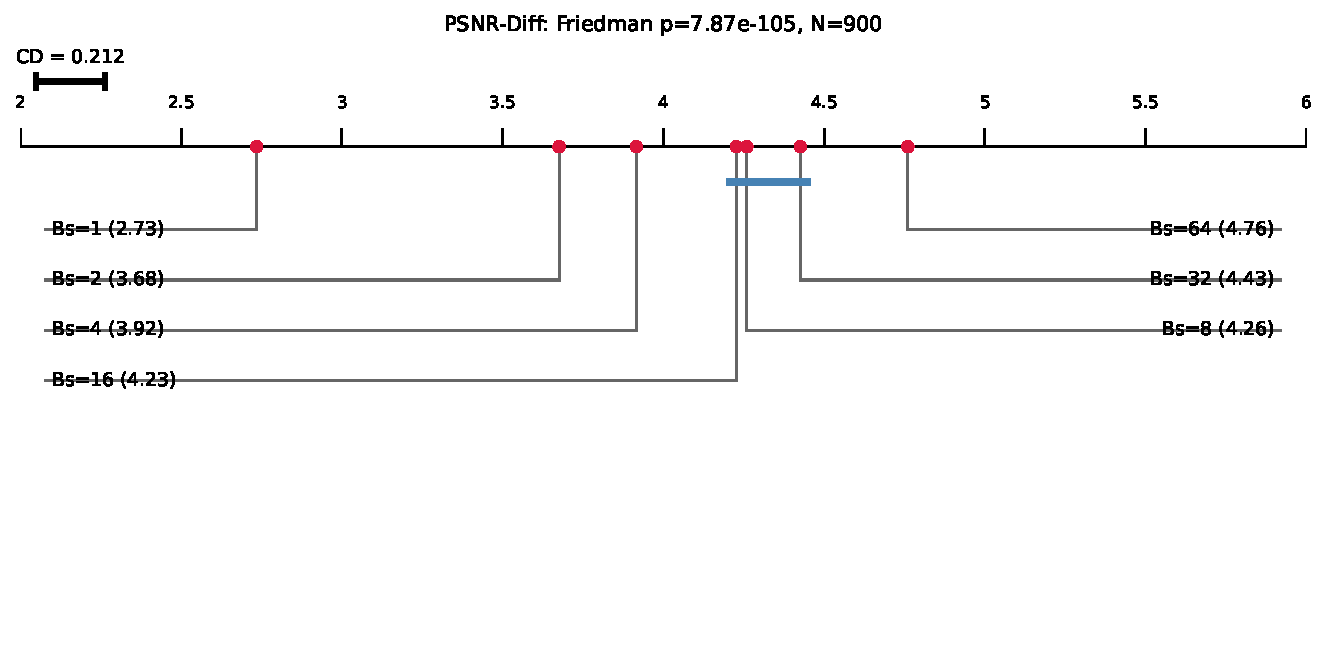
\includegraphics[width=0.85\textwidth]{Figures/CD_Bs_metric_PSNR-Diff.pdf}
\vspace{0.5em}
\hrule
\caption{Single-metric CD: PSNR-Diff, seven-buffer comparison. Artefact-removal metric, non-monotonic behaviour favouring smaller buffers.}
\label{fig:cd_bs_psnr}
\vspace{0.5em}
\hrule
\end{figure}

\begin{figure}[!htb]
\hrule
\vspace{0.5em}
\centering
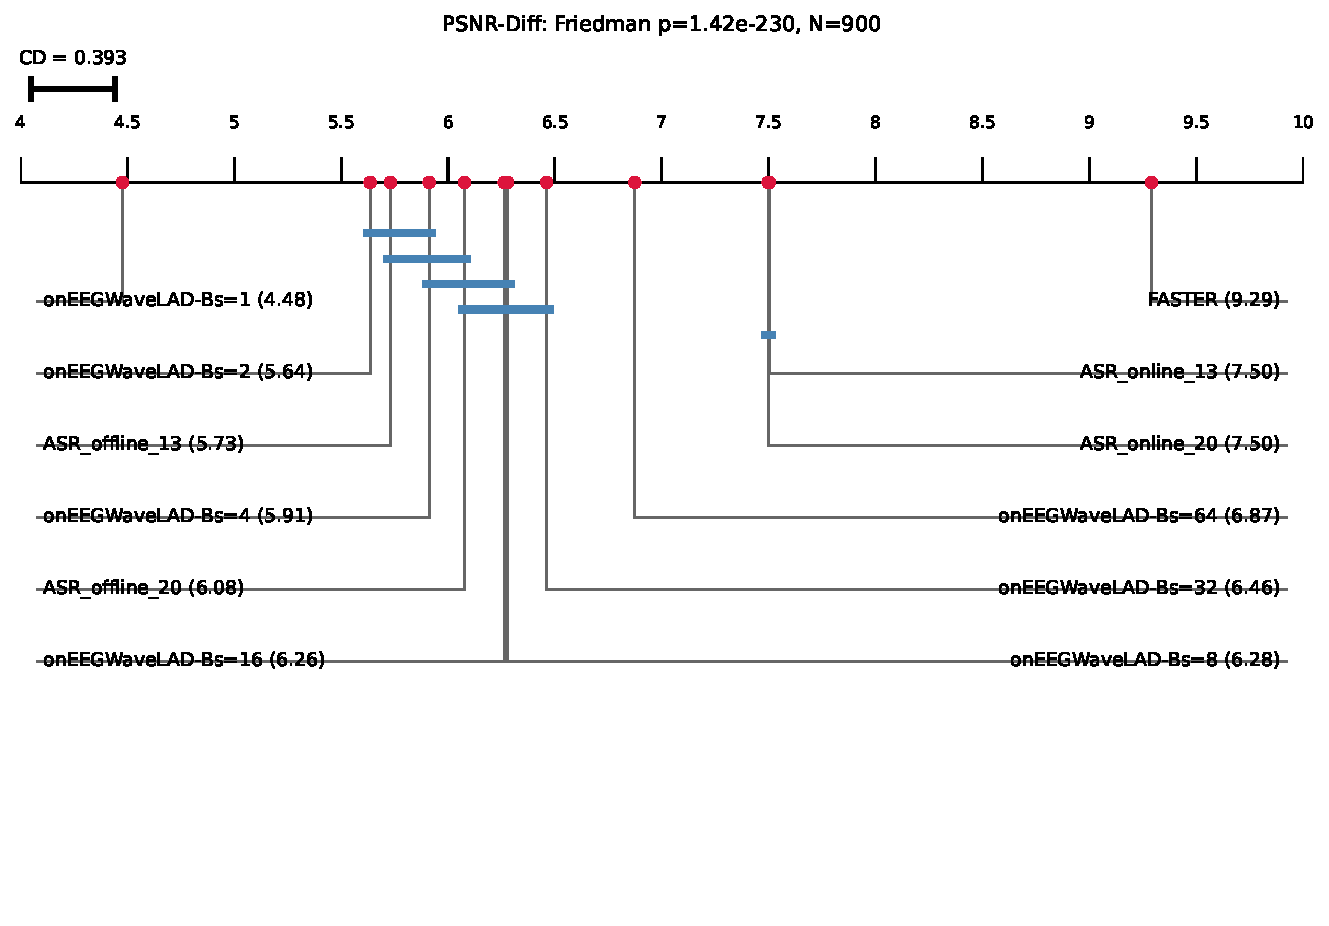
\includegraphics[width=0.95\textwidth]{Figures/CD_baseline_metric_PSNR-Diff.pdf}
\vspace{0.5em}
\hrule
\caption{Single-metric CD: PSNR-Diff, twelve-method comparison.}
\label{fig:cd_baseline_psnr}
\vspace{0.5em}
\hrule
\end{figure}

\begin{figure}[!htb]
\hrule
\vspace{0.5em}
\centering
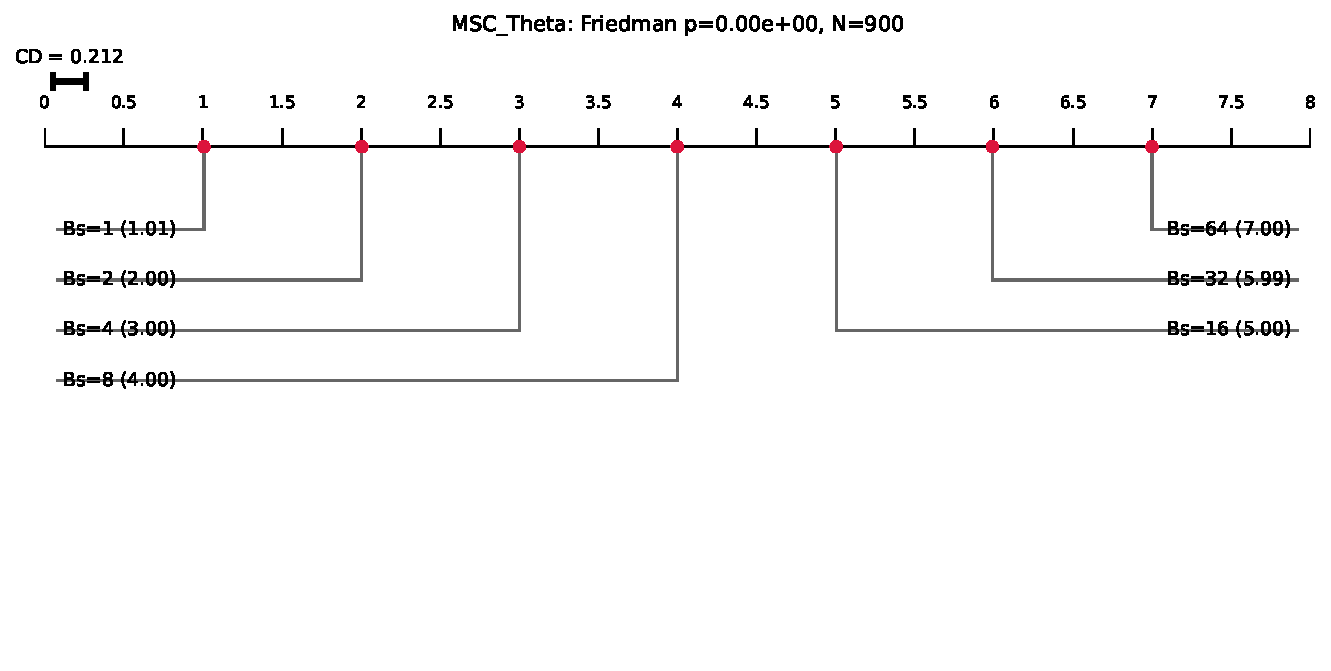
\includegraphics[width=0.85\textwidth]{Figures/CD_Bs_metric_MSC_Theta.pdf}
\vspace{0.5em}
\hrule
\caption{Single-metric CD: MSC Theta Band, seven-buffer comparison. Artefact-removal metric, non-monotonic behaviour favouring smaller buffers.}
\label{fig:cd_bs_msc_theta}
\vspace{0.5em}
\hrule
\end{figure}

\begin{figure}[!htb]
\hrule
\vspace{0.5em}
\centering
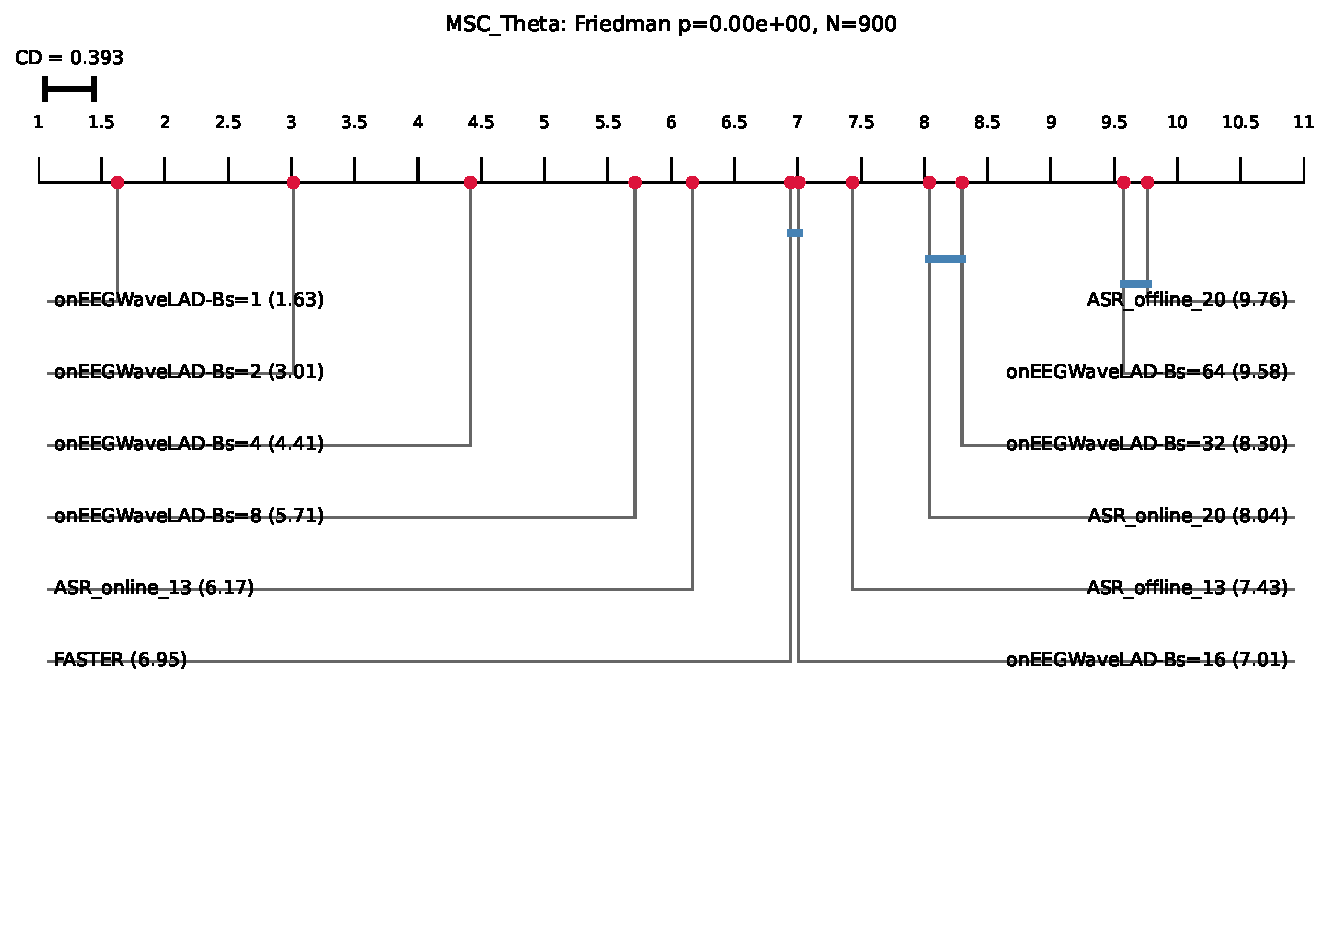
\includegraphics[width=0.95\textwidth]{Figures/CD_baseline_metric_MSC_Theta.pdf}
\vspace{0.5em}
\hrule
\caption{Single-metric CD: MSC Theta Band, twelve-method comparison.}
\label{fig:cd_baseline_msc_theta}
\vspace{0.5em}
\hrule
\end{figure}

\begin{figure}[!htb]
\hrule
\vspace{0.5em}
\centering
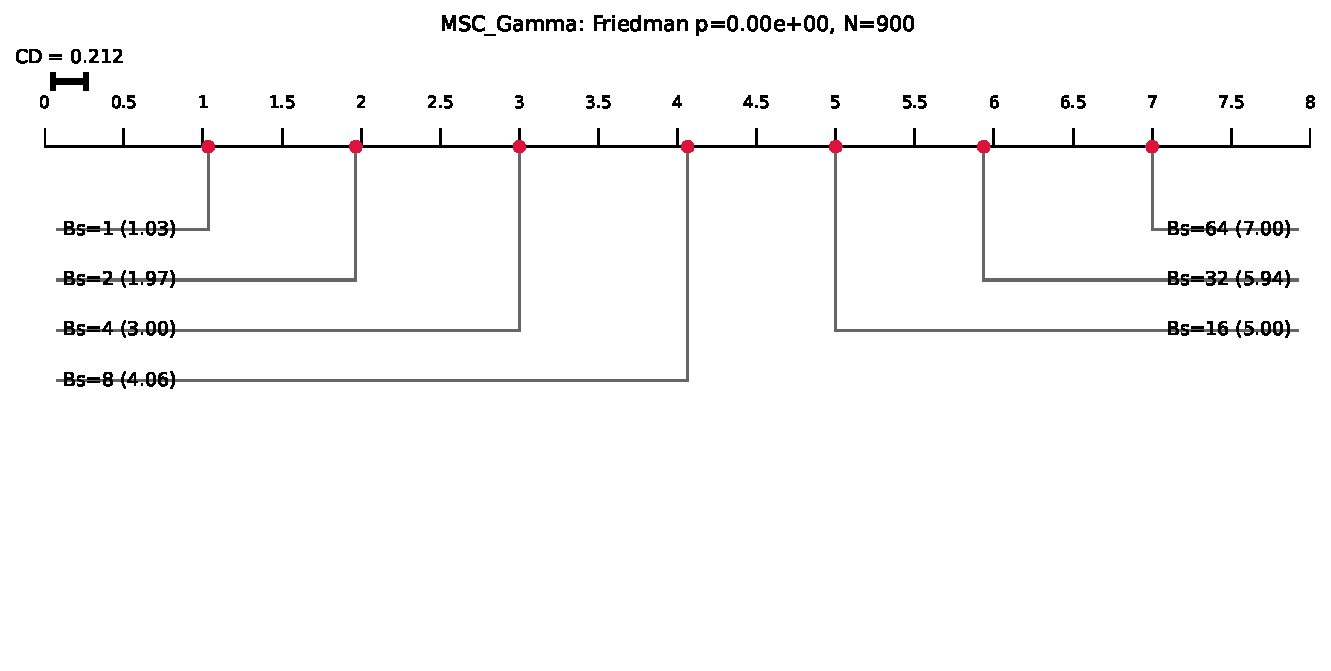
\includegraphics[width=0.85\textwidth]{Figures/CD_Bs_metric_MSC_Gamma.pdf}
\vspace{0.5em}
\hrule
\caption{Single-metric CD: MSC Gamma Band, seven-buffer comparison. Artefact-removal metric, non-monotonic behaviour favouring smaller buffers.}
\label{fig:cd_bs_msc_gamma}
\vspace{0.5em}
\hrule
\end{figure}

\begin{figure}[!htb]
\hrule
\vspace{0.5em}
\centering
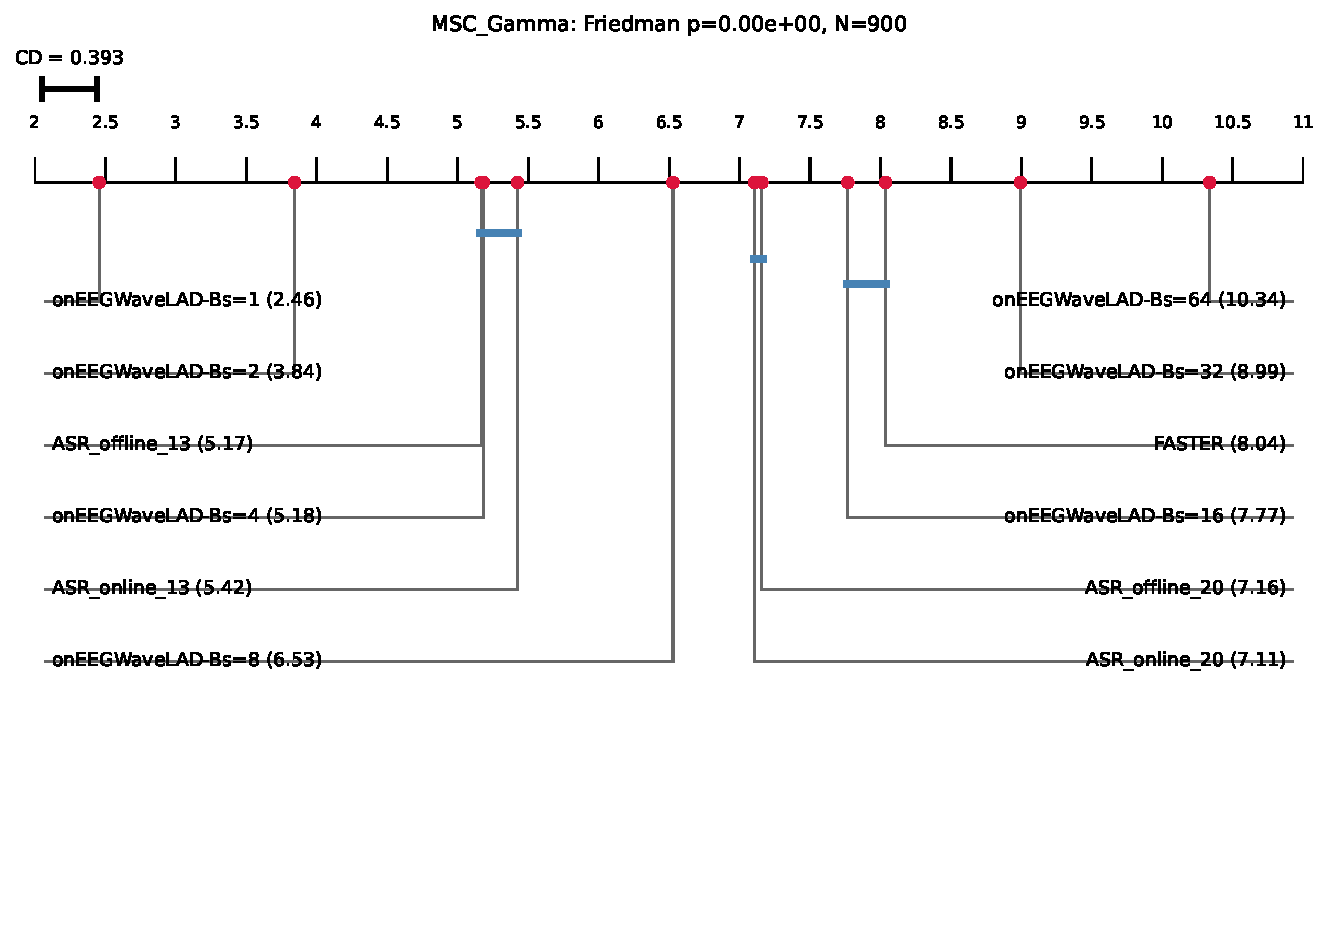
\includegraphics[width=0.95\textwidth]{Figures/CD_baseline_metric_MSC_Gamma.pdf}
\vspace{0.5em}
\hrule
\caption{Single-metric CD: MSC Gamma Band, twelve-method comparison.}
\label{fig:cd_baseline_msc_gamma}
\vspace{0.5em}
\hrule
\end{figure}

\begin{figure}[!htb]
\hrule
\vspace{0.5em}
\centering
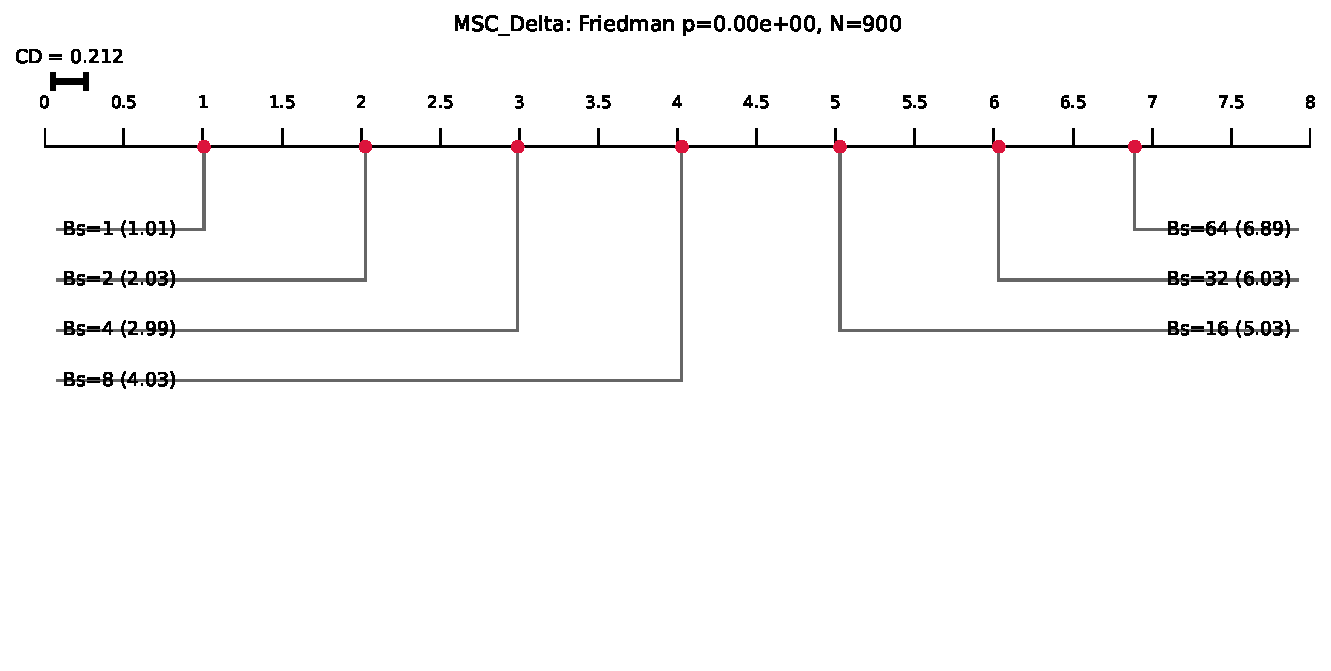
\includegraphics[width=0.85\textwidth]{Figures/CD_Bs_metric_MSC_Delta.pdf}
\vspace{0.5em}
\hrule
\caption{Single-metric CD: MSC Delta Band, seven-buffer comparison. Artefact-removal metric, non-monotonic behaviour favouring smaller buffers.}
\label{fig:cd_bs_msc_delta}
\vspace{0.5em}
\hrule
\end{figure}

\begin{figure}[!htb]
\hrule
\vspace{0.5em}
\centering
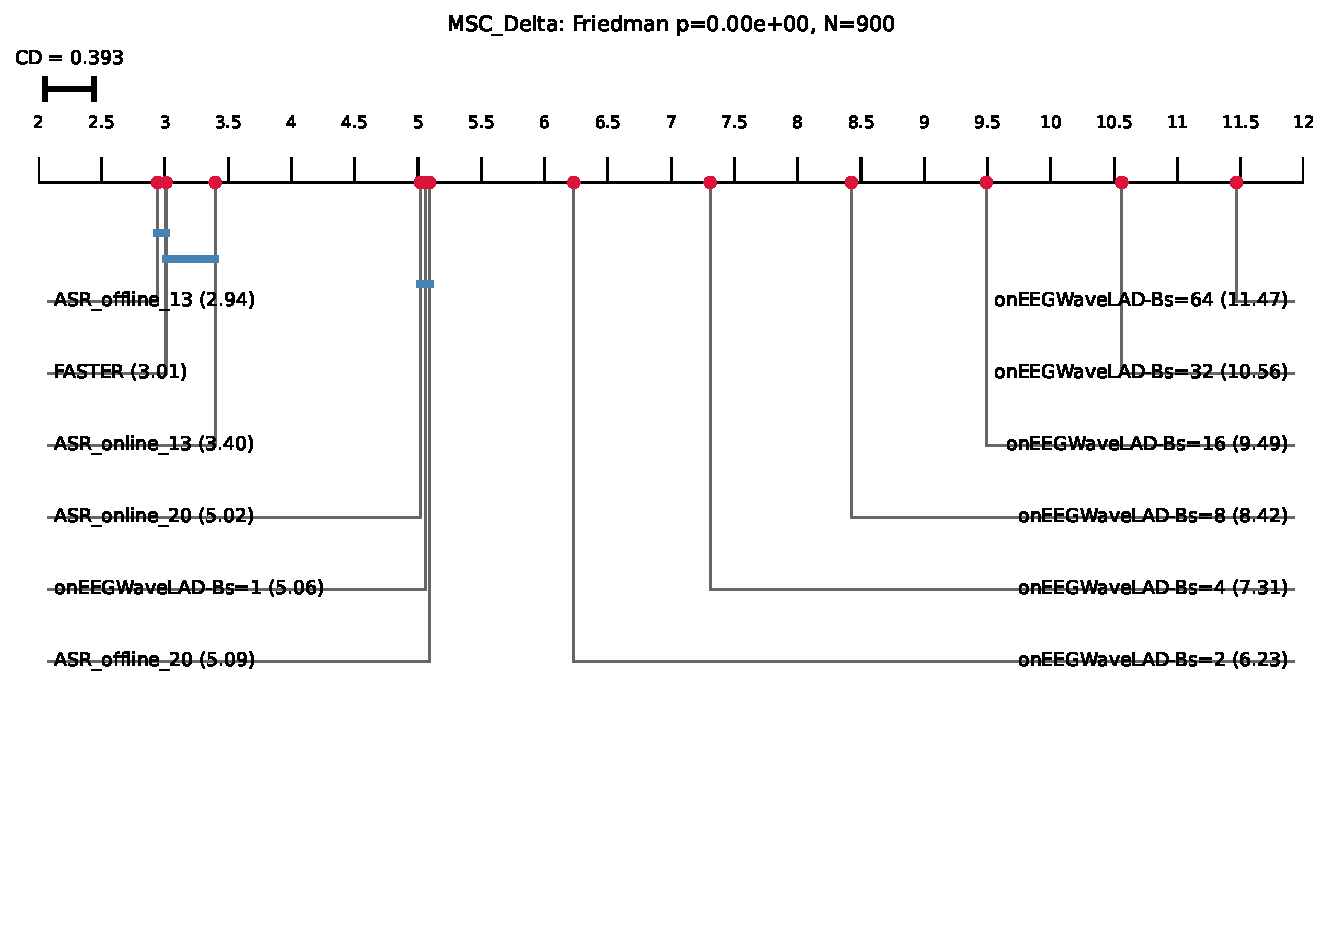
\includegraphics[width=0.95\textwidth]{Figures/CD_baseline_metric_MSC_Delta.pdf}
\vspace{0.5em}
\hrule
\caption{Single-metric CD: MSC Delta Band, twelve-method comparison.}
\label{fig:cd_baseline_msc_delta}
\vspace{0.5em}
\hrule
\end{figure}

\chapter{Core Code Implementations}
\label{app:code}

This appendix presents key code snippets from the implementation of the onEEGwaveLAD evaluation pipeline. The complete codebase is available in the project repository. All code is written in Python 3.9+ and relies on the scientific libraries detailed in Section~\ref{sec:deployment_environment}.

\section{Streaming Emulation and Windowing}
\label{app:code_streaming}

The windowing mechanism segments continuous EEG into non-overlapping blocks aligned to power-of-two boundaries for efficient DWT computation.

\begin{lstlisting}[language=Python, caption={Core windowing logic}, label={lst:streaming}]
# Align window size to nearest power of 2 for DWT efficiency
theo = (self.RTWL / 1000.0) * self.Sr
self.window_samples = int(2 ** np.ceil(np.log2(theo)))
self.actual_RTWL = (self.window_samples / self.Sr) * 1000.0

# Generate non-overlapping windows in causal order
for s in range(0, self.total_samples, self.window_samples):
    e = s + self.window_samples
    if e > self.total_samples:
        break  # Discard incomplete final window
    yield {"original_window": curr_clean, "dwt_input": curr_noisy}
\end{lstlisting}

\section{DWT and Scaleogram Construction}
\label{app:code_dwt}

Multi-level DWT decomposes the signal into detail coefficients, which are upsampled to a common temporal resolution and normalized by scale to form the scaleogram matrix.

\begin{lstlisting}[language=Python, caption={Scaleogram construction from DWT coefficients}, label={lst:dwt}]
# Multi-level DWT decomposition
coeffs = pywt.wavedec(dwt_input_data[ch], self.MW, 
                     level=actual_level, mode='periodization')

# Extract detail coefficients and build scaleogram
details = coeffs[1:]  # [cD_L, cD_{L-1}, ..., cD_1]
num_scales = len(details)
n_isps = target_len // 2

# Upsample each scale to common resolution and normalize
for i, c in enumerate(details):
    m_level = num_scales - i
    repeats = n_isps // len(c)
    upsampled = np.repeat(c, repeats)
    raw_scaleogram[:, i] = upsampled
    norm_scaleogram[:, i] = upsampled / (2 ** m_level)
\end{lstlisting}

\section{Extended Isolation Forest Integration}
\label{app:code_eiforest}

The sliding buffer stores recent ISPs, the eiFOREST model is periodically retrained, and anomaly scores are computed for the current window.

\begin{lstlisting}[language=Python, caption={Adaptive buffer management and anomaly detection}, label={lst:eiforest}]
# Score current window with existing model
if self.models[ch] is not None:
    scores = self.models[ch].predict(norm_scaleogram)
else:
    scores = np.zeros(n_isps)

# Update sliding buffer (FIFO queue)
self.moving_buffers_history[ch].append(norm_scaleogram)
if len(self.moving_buffers_history[ch]) > self.Bs:
    self.moving_buffers_history[ch].pop(0)

moving_buffer = np.vstack(self.moving_buffers_history[ch])

# Update baseline statistics
self.centroids[ch] = np.mean(moving_buffer, axis=0)
self.max_dists[ch] = np.max(
    np.abs(moving_buffer - self.centroids[ch]), axis=0
) + 1e-8

# Retrain model every 5 windows
if moving_buffer.shape[0] >= self.IFS:
    if self.models[ch] is None or self.window_cnt % 5 == 0:
        self.models[ch] = IsolationForest(
            ntrees=self.IFt, sample_size=self.IFS, 
            random_seed=42, nthreads=-1
        )
        self.models[ch].fit(moving_buffer)
\end{lstlisting}

\section{Adaptive Mitigation and Reconstruction}
\label{app:code_mitigation}

Anomalous ISPs are attenuated based on their distance from the baseline centroid, with temporal expansion of the mitigation footprint.

\begin{lstlisting}[language=Python, caption={Selective attenuation and signal reconstruction}, label={lst:mitigation}]
# Identify anomalous time points and expand footprint
anomalous_indices = np.where(scores > self.Ta)[0]
AT_exp = {idx + e for idx in anomalous_indices
          for e in range(-self.Es, self.Es + 1)
          if 0 <= idx + e < n_isps}

# Compute adaptive attenuation for each anomalous ISP
mitigator = np.ones((n_isps, num_scales))
for idx in AT_exp:
    dist_vec = np.abs(norm_scaleogram[idx] - self.centroids[ch])
    mtga_vec = 1.0 - (dist_vec / self.max_dists[ch])
    mtga_vec = np.clip(mtga_vec, 0.0, 1.0)
    mitigator[idx] = np.minimum(mitigator[idx], mtga_vec)

# Apply mitigation and reconstruct
denoised_scaleogram = raw_scaleogram * mitigator

# Downsample mitigator and apply to original coefficients
for i in range(num_scales):
    repeats = n_isps // len(details[i])
    eff_mit = mitigator[:, i].reshape(len(details[i]), repeats)[:, 0]
    reconstructed_coeffs.append(details[i] * eff_mit)

denoised_sig = pywt.waverec(reconstructed_coeffs, MW, 
                            mode='periodization')
\end{lstlisting}

\section{Metric Computation Pipeline}
\label{app:code_metrics}

Representative metric computation methods spanning time-domain, SNR enhancement, and frequency-domain evaluation.

\begin{lstlisting}[language=Python, caption={Core metric calculations}, label={lst:metrics}]
# RMSE: Root Mean Square Error
def calc_rmse(self, reference, denoised):
    return float(np.sqrt(np.mean((reference - denoised) ** 2)))

# Pearson Correlation
def calc_correlation(self, reference, denoised):
    c, _ = pearsonr(reference, denoised)
    return float(c) if np.isfinite(c) else 0.0

# SNR via ERP baseline method (reference-free)
noise_var = float(np.mean(np.var(base, axis=1)))
erp_avg = np.mean(erp, axis=0)
p_mean = float(np.mean(erp_avg ** 2))
snr = 10.0 * np.log10(p_mean / noise_var)

# Band Power Preservation Error
f, psd_ref = welch(reference, fs=self.fs, nperseg=2048)
_, psd_den = welch(denoised, fs=self.fs, nperseg=2048)
for band, (fmin, fmax) in self.bands.items():
    idx = (f >= fmin) & (f < fmax)
    p_ref[band] = float(np.trapz(psd_ref[idx], f[idx]))
    p_den[band] = float(np.trapz(psd_den[idx], f[idx]))
tot_ref, tot_den = sum(p_ref.values()), sum(p_den.values())
bppe[band] = float(abs(p_ref[band]/tot_ref - p_den[band]/tot_den))

# Magnitude Squared Coherence
f_coh, coh = coherence(reference, denoised, fs=self.fs, 
                       nperseg=2048)
idx_c = (f_coh >= fmin) & (f_coh < fmax)
msc[band] = float(np.nanmean(coh[idx_c]))
\end{lstlisting}

\section{Statistical Analysis: Friedman and Nemenyi Tests}
\label{app:code_stats}

Rank-based non-parametric analysis with Friedman global test and Nemenyi post-hoc pairwise comparisons.

\begin{lstlisting}[language=Python, caption={Friedman test and Nemenyi critical difference}, label={lst:stats}]
# Orient metrics: negate if lower=better, so larger=better always
v = df[metric].astype(float)
oriented = -v if metric in METRICS_LOWER_BETTER else v

# Rank within each (Subject, Channel, metric) cell
r = np.apply_along_axis(lambda row: rankdata(-row), 1, 
                        wide.to_numpy())

# Friedman test across k methods
R = rank_matrix  # (N x k) matrix
chi2, p = friedmanchisquare(*[R[:, j] for j in range(k)])
avg_ranks = R.mean(axis=0)

# Nemenyi critical difference
q = Q005_INF[k] / np.sqrt(2.0)  # Studentized range statistic
cd = q * np.sqrt(k * (k + 1.0) / (6.0 * N))

# Identify non-significant cliques
for i in range(k):
    j = i
    while j + 1 < k and sorted_ranks[j+1] - sorted_ranks[i] <= cd:
        j += 1
    if j > i:
        cliques.append((i, j))
\end{lstlisting}

\end{document}